\documentclass[twoside]{book}

% Packages required by doxygen
\usepackage{fixltx2e}
\usepackage{calc}
\usepackage{doxygen}
\usepackage[export]{adjustbox} % also loads graphicx
\usepackage{graphicx}
\usepackage[utf8]{inputenc}
\usepackage{makeidx}
\usepackage{multicol}
\usepackage{multirow}
\PassOptionsToPackage{warn}{textcomp}
\usepackage{textcomp}
\usepackage[nointegrals]{wasysym}
\usepackage[table]{xcolor}

% Font selection
\usepackage[T1]{fontenc}
\usepackage[scaled=.90]{helvet}
\usepackage{courier}
\usepackage{amssymb}
\usepackage{sectsty}
\renewcommand{\familydefault}{\sfdefault}
\allsectionsfont{%
  \fontseries{bc}\selectfont%
  \color{darkgray}%
}
\renewcommand{\DoxyLabelFont}{%
  \fontseries{bc}\selectfont%
  \color{darkgray}%
}
\newcommand{\+}{\discretionary{\mbox{\scriptsize$\hookleftarrow$}}{}{}}

% Page & text layout
\usepackage{geometry}
\geometry{%
  a4paper,%
  top=2.5cm,%
  bottom=2.5cm,%
  left=2.5cm,%
  right=2.5cm%
}
\tolerance=750
\hfuzz=15pt
\hbadness=750
\setlength{\emergencystretch}{15pt}
\setlength{\parindent}{0cm}
\setlength{\parskip}{3ex plus 2ex minus 2ex}
\makeatletter
\renewcommand{\paragraph}{%
  \@startsection{paragraph}{4}{0ex}{-1.0ex}{1.0ex}{%
    \normalfont\normalsize\bfseries\SS@parafont%
  }%
}
\renewcommand{\subparagraph}{%
  \@startsection{subparagraph}{5}{0ex}{-1.0ex}{1.0ex}{%
    \normalfont\normalsize\bfseries\SS@subparafont%
  }%
}
\makeatother

% Headers & footers
\usepackage{fancyhdr}
\pagestyle{fancyplain}
\fancyhead[LE]{\fancyplain{}{\bfseries\thepage}}
\fancyhead[CE]{\fancyplain{}{}}
\fancyhead[RE]{\fancyplain{}{\bfseries\leftmark}}
\fancyhead[LO]{\fancyplain{}{\bfseries\rightmark}}
\fancyhead[CO]{\fancyplain{}{}}
\fancyhead[RO]{\fancyplain{}{\bfseries\thepage}}
\fancyfoot[LE]{\fancyplain{}{}}
\fancyfoot[CE]{\fancyplain{}{}}
\fancyfoot[RE]{\fancyplain{}{\bfseries\scriptsize Generated by Doxygen }}
\fancyfoot[LO]{\fancyplain{}{\bfseries\scriptsize Generated by Doxygen }}
\fancyfoot[CO]{\fancyplain{}{}}
\fancyfoot[RO]{\fancyplain{}{}}
\renewcommand{\footrulewidth}{0.4pt}
\renewcommand{\chaptermark}[1]{%
  \markboth{#1}{}%
}
\renewcommand{\sectionmark}[1]{%
  \markright{\thesection\ #1}%
}

% Indices & bibliography
\usepackage{natbib}
\usepackage[titles]{tocloft}
\setcounter{tocdepth}{3}
\setcounter{secnumdepth}{5}
\makeindex

% Hyperlinks (required, but should be loaded last)
\usepackage{ifpdf}
\ifpdf
  \usepackage[pdftex,pagebackref=true]{hyperref}
\else
  \usepackage[ps2pdf,pagebackref=true]{hyperref}
\fi
\hypersetup{%
  colorlinks=true,%
  linkcolor=blue,%
  citecolor=blue,%
  unicode%
}

% Custom commands
\newcommand{\clearemptydoublepage}{%
  \newpage{\pagestyle{empty}\cleardoublepage}%
}

\usepackage{caption}
\captionsetup{labelsep=space,justification=centering,font={bf},singlelinecheck=off,skip=4pt,position=top}

%===== C O N T E N T S =====

\begin{document}

% Titlepage & ToC
\hypersetup{pageanchor=false,
             bookmarksnumbered=true,
             pdfencoding=unicode
            }
\pagenumbering{alph}
\begin{titlepage}
\vspace*{7cm}
\begin{center}%
{\Large libxputty \\[1ex]\large 0.\+1 }\\
\vspace*{1cm}
{\large Generated by Doxygen 1.8.13}\\
\end{center}
\end{titlepage}
\clearemptydoublepage
\pagenumbering{roman}
\tableofcontents
\clearemptydoublepage
\pagenumbering{arabic}
\hypersetup{pageanchor=true}

%--- Begin generated contents ---
\chapter{Xputty}
\label{index}\hypertarget{index}{}A damn tiny abstraction Layer to create X11 window/widgets with cairo surfaces

\subsection*{Features}


\begin{DoxyItemize}
\item easy creation of widgets and windows within the xlib windows system
\item easy handling of multiple windows including multiple widgets
\item easy to use main struct to handle the lifetime of all widgets and windows
\begin{DoxyItemize}
\item \hyperlink{structXputty}{Xputty} main;
\item main\+\_\+init(\&main);
\item create\+\_\+windows();
\item main\+\_\+run(\&main);
\item main\+\_\+quit(\&main);
\end{DoxyItemize}
\item easy connection to event handlers by simply overwriting the defaults with you own handlers
\item double buffered cairo surfaces to enable transparent drawing on child widgets
\item easy to use x/y adjustments to create your own controller widgets like sliders, knobs, buttons or a trackball
\item full documented A\+PI \href{https://brummer10.github.io/Xputty/html/index.html}{\tt Documentation}
\item static linking to create position independent applications
\end{DoxyItemize}

Here is the usual hello world\+:



produced by this code\+:


\begin{DoxyCode}
\textcolor{preprocessor}{#include "\hyperlink{xputty_8h}{xputty.h}"}
\textcolor{comment}{}
\textcolor{comment}{/** your own expose function */}
\textcolor{keyword}{static} \textcolor{keywordtype}{void} draw\_window(\textcolor{keywordtype}{void} *w\_, \textcolor{keywordtype}{void}* user\_data) \{
    \hyperlink{structWidget__t}{Widget\_t} *w = (\hyperlink{structWidget__t}{Widget\_t}*)w\_;
    cairo\_set\_source\_rgb (w->\hyperlink{structWidget__t_ad98022ee160d4c0906110868fc9e5664}{crb}, 1, 1, 1);
    cairo\_paint (w->\hyperlink{structWidget__t_ad98022ee160d4c0906110868fc9e5664}{crb});
\}

\textcolor{keywordtype}{int} main (\textcolor{keywordtype}{int} argc, \textcolor{keywordtype}{char} ** argv)
\{\textcolor{comment}{}
\textcolor{comment}{    /** acces the main struct */}
    \hyperlink{structXputty}{Xputty} app;\textcolor{comment}{}
\textcolor{comment}{    /** init the main struct */}
    \hyperlink{xputty_8c_a484645d624d9e9eff0288f8d5583ff5e}{main\_init}(&app);\textcolor{comment}{}
\textcolor{comment}{    /** create a Window on default root window */}
    \hyperlink{structWidget__t}{Widget\_t} *w = \hyperlink{xwidget_8c_a5528f841e6b5f2ef62b3b10bfa8bf20f}{create\_window}(&app, DefaultRootWindow(app.
      \hyperlink{structXputty_ab185ae4fd00ee1930c61e0440734878f}{dpy}), 0, 0, 300, 200);\textcolor{comment}{}
\textcolor{comment}{    /** acces Xlib function */}
    XStoreName(app.\hyperlink{structXputty_ab185ae4fd00ee1930c61e0440734878f}{dpy}, w->\hyperlink{structWidget__t_acb2bfb41674371ee1220a9d6a2d89fb1}{widget}, \textcolor{stringliteral}{"Hello world"});\textcolor{comment}{}
\textcolor{comment}{    /** overwrite event handler with your own */}
    w->\hyperlink{structWidget__t_a225b9a175e132994a5aa73b59a2911ad}{func}.\hyperlink{structFunc__t_ae4ba307ec29bfea83e1197aa750c1396}{expose\_callback} = draw\_window;\textcolor{comment}{}
\textcolor{comment}{    /** map the Window to display */}
    \hyperlink{xwidget_8c_aae228a75c93bb0cb9ad57ffaf4d25922}{widget\_show\_all}(w);\textcolor{comment}{}
\textcolor{comment}{    /** run the event loop */}
    \hyperlink{xputty_8c_abb548ea64f852a7c94473a595e67d69f}{main\_run}(&app);\textcolor{comment}{}
\textcolor{comment}{    /** clean up after the event loop is finished */}
    \hyperlink{xputty_8c_a0d4eda902b4de6f7a30e8d869f842fda}{main\_quit}(&app);
    \textcolor{keywordflow}{return} 0;
\}
\end{DoxyCode}


check out the example folder for more examples.

\subsection*{License}

\begin{DoxyVerb}     0BSD 
\end{DoxyVerb}
 B\+SD Zero Clause License 
\chapter{Data Structure Index}
\section{Data Structures}
Here are the data structures with brief descriptions\+:\begin{DoxyCompactList}
\item\contentsline{section}{\hyperlink{structAdjustment__t}{Adjustment\+\_\+t} \\*\hyperlink{structAdjustment__t}{Adjustment\+\_\+t} -\/ struct to hold a controller adjustment }{\pageref{structAdjustment__t}}{}
\item\contentsline{section}{\hyperlink{structChildlist__t}{Childlist\+\_\+t} \\*\hyperlink{structChildlist__t}{Childlist\+\_\+t} -\/ struct to hold a \hyperlink{structWidget__t}{Widget\+\_\+t} child list }{\pageref{structChildlist__t}}{}
\item\contentsline{section}{\hyperlink{structFunc__t}{Func\+\_\+t} \\*\hyperlink{structFunc__t}{Func\+\_\+t} -\/ struct to hold all supported event callbacks }{\pageref{structFunc__t}}{}
\item\contentsline{section}{\hyperlink{structResize__t}{Resize\+\_\+t} \\*\hyperlink{structResize__t}{Resize\+\_\+t} -\/ struct used to resize child widgets }{\pageref{structResize__t}}{}
\item\contentsline{section}{\hyperlink{structWidget__t}{Widget\+\_\+t} \\*\hyperlink{structWidget__t}{Widget\+\_\+t} -\/ struct to hold the basic widget info }{\pageref{structWidget__t}}{}
\item\contentsline{section}{\hyperlink{structXputty}{Xputty} \\*\hyperlink{structXputty}{Xputty} -\/ the main struct }{\pageref{structXputty}}{}
\end{DoxyCompactList}

\chapter{File Index}
\section{File List}
Here is a list of all files with brief descriptions\+:\begin{DoxyCompactList}
\item\contentsline{section}{\hyperlink{xadjustment_8c}{xadjustment.\+c} }{\pageref{xadjustment_8c}}{}
\item\contentsline{section}{\hyperlink{xadjustment_8h}{xadjustment.\+h} }{\pageref{xadjustment_8h}}{}
\item\contentsline{section}{\hyperlink{xadjustment__private_8c}{xadjustment\+\_\+private.\+c} }{\pageref{xadjustment__private_8c}}{}
\item\contentsline{section}{\hyperlink{xadjustment__private_8h}{xadjustment\+\_\+private.\+h} }{\pageref{xadjustment__private_8h}}{}
\item\contentsline{section}{\hyperlink{xbutton_8c}{xbutton.\+c} }{\pageref{xbutton_8c}}{}
\item\contentsline{section}{\hyperlink{xbutton_8h}{xbutton.\+h} }{\pageref{xbutton_8h}}{}
\item\contentsline{section}{\hyperlink{xbutton__private_8c}{xbutton\+\_\+private.\+c} }{\pageref{xbutton__private_8c}}{}
\item\contentsline{section}{\hyperlink{xbutton__private_8h}{xbutton\+\_\+private.\+h} }{\pageref{xbutton__private_8h}}{}
\item\contentsline{section}{\hyperlink{xchildlist_8c}{xchildlist.\+c} }{\pageref{xchildlist_8c}}{}
\item\contentsline{section}{\hyperlink{xchildlist_8h}{xchildlist.\+h} }{\pageref{xchildlist_8h}}{}
\item\contentsline{section}{\hyperlink{xchildlist__private_8c}{xchildlist\+\_\+private.\+c} }{\pageref{xchildlist__private_8c}}{}
\item\contentsline{section}{\hyperlink{xchildlist__private_8h}{xchildlist\+\_\+private.\+h} }{\pageref{xchildlist__private_8h}}{}
\item\contentsline{section}{\hyperlink{xputty_8c}{xputty.\+c} }{\pageref{xputty_8c}}{}
\item\contentsline{section}{\hyperlink{xputty_8h}{xputty.\+h} }{\pageref{xputty_8h}}{}
\item\contentsline{section}{\hyperlink{xwidget_8c}{xwidget.\+c} }{\pageref{xwidget_8c}}{}
\item\contentsline{section}{\hyperlink{xwidget_8h}{xwidget.\+h} }{\pageref{xwidget_8h}}{}
\item\contentsline{section}{\hyperlink{xwidget__private_8c}{xwidget\+\_\+private.\+c} }{\pageref{xwidget__private_8c}}{}
\item\contentsline{section}{\hyperlink{xwidget__private_8h}{xwidget\+\_\+private.\+h} }{\pageref{xwidget__private_8h}}{}
\end{DoxyCompactList}

\chapter{Data Structure Documentation}
\hypertarget{structAdjustment__t}{}\section{Adjustment\+\_\+t Struct Reference}
\label{structAdjustment__t}\index{Adjustment\+\_\+t@{Adjustment\+\_\+t}}


\hyperlink{structAdjustment__t}{Adjustment\+\_\+t} -\/ struct to hold a controller adjustment.  




{\ttfamily \#include $<$xadjustment.\+h$>$}

\subsection*{Data Fields}
\begin{DoxyCompactItemize}
\item 
float \hyperlink{structAdjustment__t_ab90ff6647e5933aa4919724d61e15e23}{std\+\_\+value}
\item 
float \hyperlink{structAdjustment__t_acb1f8fb06d9e505f9f50e9178256215c}{value}
\item 
float \hyperlink{structAdjustment__t_a3ba8294662db07d7dd7ebd751b01e7a3}{min\+\_\+value}
\item 
float \hyperlink{structAdjustment__t_a8607f7be566c21036c396201bce07a1a}{max\+\_\+value}
\item 
float \hyperlink{structAdjustment__t_a0198d0a412f8642b3e8a308f9240d467}{step}
\item 
float \hyperlink{structAdjustment__t_abec8df43db1df5d6fcc6b6619773dbc9}{start\+\_\+value}
\item 
int \hyperlink{structAdjustment__t_a8d34edf1dfeaf75b7d22fb371c9c3b4a}{type}
\end{DoxyCompactItemize}


\subsection{Detailed Description}
\hyperlink{structAdjustment__t}{Adjustment\+\_\+t} -\/ struct to hold a controller adjustment. 


\begin{DoxyParams}{Parameters}
{\em std\+\_\+value} & -\/ the standart value for the adjustment \\
\hline
{\em value} & -\/ the current value of the adjustment \\
\hline
{\em min\+\_\+value} & -\/ the minimal value of the adjustment \\
\hline
{\em max\+\_\+value} & -\/ the maximal value of the adjustment \\
\hline
{\em step} & -\/ the step to increase/decrease the adjustment \\
\hline
{\em start\+\_\+value} & -\/ the value of init the adjustment with \\
\hline
{\em type} & -\/ should be on of the C\+L\+\_\+ types \\
\hline
\end{DoxyParams}


\subsection{Field Documentation}
\mbox{\Hypertarget{structAdjustment__t_a8607f7be566c21036c396201bce07a1a}\label{structAdjustment__t_a8607f7be566c21036c396201bce07a1a}} 
\index{Adjustment\+\_\+t@{Adjustment\+\_\+t}!max\+\_\+value@{max\+\_\+value}}
\index{max\+\_\+value@{max\+\_\+value}!Adjustment\+\_\+t@{Adjustment\+\_\+t}}
\subsubsection{\texorpdfstring{max\+\_\+value}{max\_value}}
{\footnotesize\ttfamily float Adjustment\+\_\+t\+::max\+\_\+value}

\mbox{\Hypertarget{structAdjustment__t_a3ba8294662db07d7dd7ebd751b01e7a3}\label{structAdjustment__t_a3ba8294662db07d7dd7ebd751b01e7a3}} 
\index{Adjustment\+\_\+t@{Adjustment\+\_\+t}!min\+\_\+value@{min\+\_\+value}}
\index{min\+\_\+value@{min\+\_\+value}!Adjustment\+\_\+t@{Adjustment\+\_\+t}}
\subsubsection{\texorpdfstring{min\+\_\+value}{min\_value}}
{\footnotesize\ttfamily float Adjustment\+\_\+t\+::min\+\_\+value}

\mbox{\Hypertarget{structAdjustment__t_abec8df43db1df5d6fcc6b6619773dbc9}\label{structAdjustment__t_abec8df43db1df5d6fcc6b6619773dbc9}} 
\index{Adjustment\+\_\+t@{Adjustment\+\_\+t}!start\+\_\+value@{start\+\_\+value}}
\index{start\+\_\+value@{start\+\_\+value}!Adjustment\+\_\+t@{Adjustment\+\_\+t}}
\subsubsection{\texorpdfstring{start\+\_\+value}{start\_value}}
{\footnotesize\ttfamily float Adjustment\+\_\+t\+::start\+\_\+value}

\mbox{\Hypertarget{structAdjustment__t_ab90ff6647e5933aa4919724d61e15e23}\label{structAdjustment__t_ab90ff6647e5933aa4919724d61e15e23}} 
\index{Adjustment\+\_\+t@{Adjustment\+\_\+t}!std\+\_\+value@{std\+\_\+value}}
\index{std\+\_\+value@{std\+\_\+value}!Adjustment\+\_\+t@{Adjustment\+\_\+t}}
\subsubsection{\texorpdfstring{std\+\_\+value}{std\_value}}
{\footnotesize\ttfamily float Adjustment\+\_\+t\+::std\+\_\+value}

\mbox{\Hypertarget{structAdjustment__t_a0198d0a412f8642b3e8a308f9240d467}\label{structAdjustment__t_a0198d0a412f8642b3e8a308f9240d467}} 
\index{Adjustment\+\_\+t@{Adjustment\+\_\+t}!step@{step}}
\index{step@{step}!Adjustment\+\_\+t@{Adjustment\+\_\+t}}
\subsubsection{\texorpdfstring{step}{step}}
{\footnotesize\ttfamily float Adjustment\+\_\+t\+::step}

\mbox{\Hypertarget{structAdjustment__t_a8d34edf1dfeaf75b7d22fb371c9c3b4a}\label{structAdjustment__t_a8d34edf1dfeaf75b7d22fb371c9c3b4a}} 
\index{Adjustment\+\_\+t@{Adjustment\+\_\+t}!type@{type}}
\index{type@{type}!Adjustment\+\_\+t@{Adjustment\+\_\+t}}
\subsubsection{\texorpdfstring{type}{type}}
{\footnotesize\ttfamily int Adjustment\+\_\+t\+::type}

\mbox{\Hypertarget{structAdjustment__t_acb1f8fb06d9e505f9f50e9178256215c}\label{structAdjustment__t_acb1f8fb06d9e505f9f50e9178256215c}} 
\index{Adjustment\+\_\+t@{Adjustment\+\_\+t}!value@{value}}
\index{value@{value}!Adjustment\+\_\+t@{Adjustment\+\_\+t}}
\subsubsection{\texorpdfstring{value}{value}}
{\footnotesize\ttfamily float Adjustment\+\_\+t\+::value}



The documentation for this struct was generated from the following file\+:\begin{DoxyCompactItemize}
\item 
\hyperlink{xadjustment_8h}{xadjustment.\+h}\end{DoxyCompactItemize}

\hypertarget{structChildlist__t}{}\section{Childlist\+\_\+t Struct Reference}
\label{structChildlist__t}\index{Childlist\+\_\+t@{Childlist\+\_\+t}}


\hyperlink{structChildlist__t}{Childlist\+\_\+t} -\/ struct to hold a \hyperlink{structWidget__t}{Widget\+\_\+t} child list.  




{\ttfamily \#include $<$xchildlist.\+h$>$}



Collaboration diagram for Childlist\+\_\+t\+:
\nopagebreak
\begin{figure}[H]
\begin{center}
\leavevmode
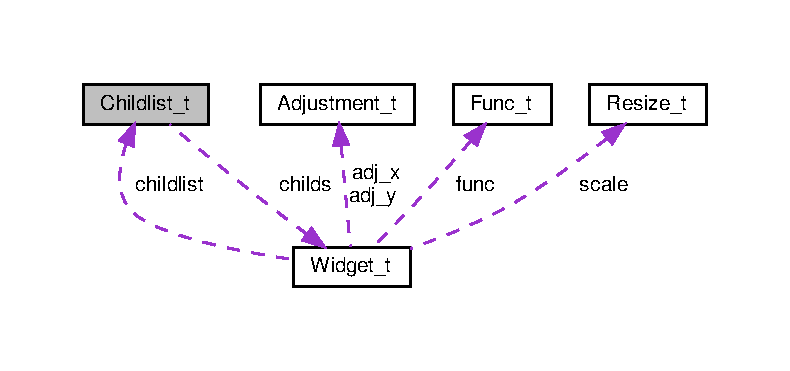
\includegraphics[width=311pt]{structChildlist__t__coll__graph}
\end{center}
\end{figure}
\subsection*{Data Fields}
\begin{DoxyCompactItemize}
\item 
\hyperlink{structWidget__t}{Widget\+\_\+t} $\ast$$\ast$ \hyperlink{structChildlist__t_a093a27797dc1a2819546ceb857b3db1a}{childs}
\item 
size\+\_\+t \hyperlink{structChildlist__t_a3045339822c393689c6fac8b8a2a4457}{size}
\item 
int \hyperlink{structChildlist__t_abf81fe823696baae53ff77036227f0c8}{cap}
\item 
int \hyperlink{structChildlist__t_a5d7a8d584c55c0496e5710d9a6f4282f}{elem}
\end{DoxyCompactItemize}


\subsection{Detailed Description}
\hyperlink{structChildlist__t}{Childlist\+\_\+t} -\/ struct to hold a \hyperlink{structWidget__t}{Widget\+\_\+t} child list. 


\begin{DoxyParams}{Parameters}
{\em $\ast$$\ast$childs} & -\/ dynamic array to hold pointers to the childs \\
\hline
{\em size} & -\/ current size of array \\
\hline
{\em cap} & -\/ current capacity of the array \\
\hline
{\em elem} & -\/ current elements in the array \\
\hline
\end{DoxyParams}


\subsection{Field Documentation}
\mbox{\Hypertarget{structChildlist__t_abf81fe823696baae53ff77036227f0c8}\label{structChildlist__t_abf81fe823696baae53ff77036227f0c8}} 
\index{Childlist\+\_\+t@{Childlist\+\_\+t}!cap@{cap}}
\index{cap@{cap}!Childlist\+\_\+t@{Childlist\+\_\+t}}
\subsubsection{\texorpdfstring{cap}{cap}}
{\footnotesize\ttfamily int Childlist\+\_\+t\+::cap}

\mbox{\Hypertarget{structChildlist__t_a093a27797dc1a2819546ceb857b3db1a}\label{structChildlist__t_a093a27797dc1a2819546ceb857b3db1a}} 
\index{Childlist\+\_\+t@{Childlist\+\_\+t}!childs@{childs}}
\index{childs@{childs}!Childlist\+\_\+t@{Childlist\+\_\+t}}
\subsubsection{\texorpdfstring{childs}{childs}}
{\footnotesize\ttfamily \hyperlink{structWidget__t}{Widget\+\_\+t}$\ast$$\ast$ Childlist\+\_\+t\+::childs}

\mbox{\Hypertarget{structChildlist__t_a5d7a8d584c55c0496e5710d9a6f4282f}\label{structChildlist__t_a5d7a8d584c55c0496e5710d9a6f4282f}} 
\index{Childlist\+\_\+t@{Childlist\+\_\+t}!elem@{elem}}
\index{elem@{elem}!Childlist\+\_\+t@{Childlist\+\_\+t}}
\subsubsection{\texorpdfstring{elem}{elem}}
{\footnotesize\ttfamily int Childlist\+\_\+t\+::elem}

\mbox{\Hypertarget{structChildlist__t_a3045339822c393689c6fac8b8a2a4457}\label{structChildlist__t_a3045339822c393689c6fac8b8a2a4457}} 
\index{Childlist\+\_\+t@{Childlist\+\_\+t}!size@{size}}
\index{size@{size}!Childlist\+\_\+t@{Childlist\+\_\+t}}
\subsubsection{\texorpdfstring{size}{size}}
{\footnotesize\ttfamily size\+\_\+t Childlist\+\_\+t\+::size}



The documentation for this struct was generated from the following file\+:\begin{DoxyCompactItemize}
\item 
\hyperlink{xchildlist_8h}{xchildlist.\+h}\end{DoxyCompactItemize}

\hypertarget{structColor__t}{}\section{Color\+\_\+t Struct Reference}
\label{structColor__t}\index{Color\+\_\+t@{Color\+\_\+t}}


\hyperlink{structColor__t}{Color\+\_\+t} -\/ struct used to set cairo color for \hyperlink{structWidget__t}{Widget\+\_\+t}.  




{\ttfamily \#include $<$xwidget.\+h$>$}

\subsection*{Data Fields}
\begin{DoxyCompactItemize}
\item 
float \hyperlink{structColor__t_a5491170cc9c33b98a7c0e8a4a25f4c0a}{fg} \mbox{[}4\mbox{]}
\item 
float \hyperlink{structColor__t_acf62f86fb2579ce93a4e942ded82ab32}{bg} \mbox{[}4\mbox{]}
\item 
float \hyperlink{structColor__t_a6d10838bcc8244d773f3c44b321016b8}{ba} \mbox{[}4\mbox{]}
\end{DoxyCompactItemize}


\subsection{Detailed Description}
\hyperlink{structColor__t}{Color\+\_\+t} -\/ struct used to set cairo color for \hyperlink{structWidget__t}{Widget\+\_\+t}. 


\begin{DoxyParams}{Parameters}
{\em fg\mbox{[}4\mbox{]}} & -\/ forground \{red, green, blue, alpha\} \\
\hline
{\em bg\mbox{[}4\mbox{]}} & -\/ background \{red, green, blue, alpha\} \\
\hline
{\em ba\mbox{[}4\mbox{]}} & -\/ base \{red, green, blue, alpha\} \\
\hline
\end{DoxyParams}


\subsection{Field Documentation}
\mbox{\Hypertarget{structColor__t_a6d10838bcc8244d773f3c44b321016b8}\label{structColor__t_a6d10838bcc8244d773f3c44b321016b8}} 
\index{Color\+\_\+t@{Color\+\_\+t}!ba@{ba}}
\index{ba@{ba}!Color\+\_\+t@{Color\+\_\+t}}
\subsubsection{\texorpdfstring{ba}{ba}}
{\footnotesize\ttfamily float Color\+\_\+t\+::ba\mbox{[}4\mbox{]}}

\mbox{\Hypertarget{structColor__t_acf62f86fb2579ce93a4e942ded82ab32}\label{structColor__t_acf62f86fb2579ce93a4e942ded82ab32}} 
\index{Color\+\_\+t@{Color\+\_\+t}!bg@{bg}}
\index{bg@{bg}!Color\+\_\+t@{Color\+\_\+t}}
\subsubsection{\texorpdfstring{bg}{bg}}
{\footnotesize\ttfamily float Color\+\_\+t\+::bg\mbox{[}4\mbox{]}}

\mbox{\Hypertarget{structColor__t_a5491170cc9c33b98a7c0e8a4a25f4c0a}\label{structColor__t_a5491170cc9c33b98a7c0e8a4a25f4c0a}} 
\index{Color\+\_\+t@{Color\+\_\+t}!fg@{fg}}
\index{fg@{fg}!Color\+\_\+t@{Color\+\_\+t}}
\subsubsection{\texorpdfstring{fg}{fg}}
{\footnotesize\ttfamily float Color\+\_\+t\+::fg\mbox{[}4\mbox{]}}



The documentation for this struct was generated from the following file\+:\begin{DoxyCompactItemize}
\item 
\hyperlink{xwidget_8h}{xwidget.\+h}\end{DoxyCompactItemize}

\hypertarget{structFunc__t}{}\section{Func\+\_\+t Struct Reference}
\label{structFunc__t}\index{Func\+\_\+t@{Func\+\_\+t}}


\hyperlink{structFunc__t}{Func\+\_\+t} -\/ struct to hold all supported event callbacks.  




{\ttfamily \#include $<$xwidget.\+h$>$}

\subsection*{Data Fields}
\begin{DoxyCompactItemize}
\item 
\hyperlink{xwidget_8h_a9ef0263424a7f5f8f6b02055fca67ddd}{xevfunc} \hyperlink{structFunc__t_ae4ba307ec29bfea83e1197aa750c1396}{expose\+\_\+callback}
\item 
\hyperlink{xwidget_8h_a9ef0263424a7f5f8f6b02055fca67ddd}{xevfunc} \hyperlink{structFunc__t_a7876670d3bb74b11ab93fe81908d04b0}{configure\+\_\+callback}
\item 
\hyperlink{xwidget_8h_a9ef0263424a7f5f8f6b02055fca67ddd}{xevfunc} \hyperlink{structFunc__t_a6ae24f219bf8eff4bd5fbdfa3f29c14d}{enter\+\_\+callback}
\item 
\hyperlink{xwidget_8h_a9ef0263424a7f5f8f6b02055fca67ddd}{xevfunc} \hyperlink{structFunc__t_a1801ba902bd7efc706d474312f960d0a}{leave\+\_\+callback}
\item 
\hyperlink{xwidget_8h_a9ef0263424a7f5f8f6b02055fca67ddd}{xevfunc} \hyperlink{structFunc__t_afe804d94b970050a9f85530408169623}{adj\+\_\+callback}
\item 
\hyperlink{xwidget_8h_a9ef0263424a7f5f8f6b02055fca67ddd}{xevfunc} \hyperlink{structFunc__t_acce396ccf3266886f0a6d28cf45761d3}{value\+\_\+changed\+\_\+callback}
\item 
\hyperlink{xwidget_8h_a9ef0263424a7f5f8f6b02055fca67ddd}{xevfunc} \hyperlink{structFunc__t_a1f089cb13a39764a1f980470a51db71b}{user\+\_\+callback}
\item 
\hyperlink{xwidget_8h_a9ef0263424a7f5f8f6b02055fca67ddd}{xevfunc} \hyperlink{structFunc__t_ac0a05a827a9cb6469cb15e7225411f16}{mem\+\_\+free\+\_\+callback}
\item 
\hyperlink{xwidget_8h_a9ef0263424a7f5f8f6b02055fca67ddd}{xevfunc} \hyperlink{structFunc__t_a63a27e3f238d08a6ca4b47b99ae04df9}{configure\+\_\+notify\+\_\+callback}
\item 
\hyperlink{xwidget_8h_a9ef0263424a7f5f8f6b02055fca67ddd}{xevfunc} \hyperlink{structFunc__t_ac9c7609befbb46b122100a10f6984b9f}{map\+\_\+notify\+\_\+callback}
\item 
\hyperlink{xwidget_8h_a9ef0263424a7f5f8f6b02055fca67ddd}{xevfunc} \hyperlink{structFunc__t_a59e76f78a37d59efa847627774ce38e9}{dialog\+\_\+callback}
\item 
\hyperlink{xwidget_8h_ab4ae973f86a383c8c0f92b709044520a}{evfunc} \hyperlink{structFunc__t_aa58bc35a1499d8cd850d2a083ad016f1}{button\+\_\+press\+\_\+callback}
\item 
\hyperlink{xwidget_8h_ab4ae973f86a383c8c0f92b709044520a}{evfunc} \hyperlink{structFunc__t_a8cb9d8135a178027675c96599ff8312e}{button\+\_\+release\+\_\+callback}
\item 
\hyperlink{xwidget_8h_ab4ae973f86a383c8c0f92b709044520a}{evfunc} \hyperlink{structFunc__t_ac2842c834907f4aeace8f404c6cc7621}{motion\+\_\+callback}
\item 
\hyperlink{xwidget_8h_ab4ae973f86a383c8c0f92b709044520a}{evfunc} \hyperlink{structFunc__t_a024ea4919029156d9415f1501cd8b0bf}{key\+\_\+press\+\_\+callback}
\item 
\hyperlink{xwidget_8h_ab4ae973f86a383c8c0f92b709044520a}{evfunc} \hyperlink{structFunc__t_a8c7138616caa404a9af064d673d7e0f8}{key\+\_\+release\+\_\+callback}
\end{DoxyCompactItemize}


\subsection{Detailed Description}
\hyperlink{structFunc__t}{Func\+\_\+t} -\/ struct to hold all supported event callbacks. 

\subsection{Field Documentation}
\mbox{\Hypertarget{structFunc__t_afe804d94b970050a9f85530408169623}\label{structFunc__t_afe804d94b970050a9f85530408169623}} 
\index{Func\+\_\+t@{Func\+\_\+t}!adj\+\_\+callback@{adj\+\_\+callback}}
\index{adj\+\_\+callback@{adj\+\_\+callback}!Func\+\_\+t@{Func\+\_\+t}}
\subsubsection{\texorpdfstring{adj\+\_\+callback}{adj\_callback}}
{\footnotesize\ttfamily \hyperlink{xwidget_8h_a9ef0263424a7f5f8f6b02055fca67ddd}{xevfunc} Func\+\_\+t\+::adj\+\_\+callback}

\mbox{\Hypertarget{structFunc__t_aa58bc35a1499d8cd850d2a083ad016f1}\label{structFunc__t_aa58bc35a1499d8cd850d2a083ad016f1}} 
\index{Func\+\_\+t@{Func\+\_\+t}!button\+\_\+press\+\_\+callback@{button\+\_\+press\+\_\+callback}}
\index{button\+\_\+press\+\_\+callback@{button\+\_\+press\+\_\+callback}!Func\+\_\+t@{Func\+\_\+t}}
\subsubsection{\texorpdfstring{button\+\_\+press\+\_\+callback}{button\_press\_callback}}
{\footnotesize\ttfamily \hyperlink{xwidget_8h_ab4ae973f86a383c8c0f92b709044520a}{evfunc} Func\+\_\+t\+::button\+\_\+press\+\_\+callback}

\mbox{\Hypertarget{structFunc__t_a8cb9d8135a178027675c96599ff8312e}\label{structFunc__t_a8cb9d8135a178027675c96599ff8312e}} 
\index{Func\+\_\+t@{Func\+\_\+t}!button\+\_\+release\+\_\+callback@{button\+\_\+release\+\_\+callback}}
\index{button\+\_\+release\+\_\+callback@{button\+\_\+release\+\_\+callback}!Func\+\_\+t@{Func\+\_\+t}}
\subsubsection{\texorpdfstring{button\+\_\+release\+\_\+callback}{button\_release\_callback}}
{\footnotesize\ttfamily \hyperlink{xwidget_8h_ab4ae973f86a383c8c0f92b709044520a}{evfunc} Func\+\_\+t\+::button\+\_\+release\+\_\+callback}

\mbox{\Hypertarget{structFunc__t_a7876670d3bb74b11ab93fe81908d04b0}\label{structFunc__t_a7876670d3bb74b11ab93fe81908d04b0}} 
\index{Func\+\_\+t@{Func\+\_\+t}!configure\+\_\+callback@{configure\+\_\+callback}}
\index{configure\+\_\+callback@{configure\+\_\+callback}!Func\+\_\+t@{Func\+\_\+t}}
\subsubsection{\texorpdfstring{configure\+\_\+callback}{configure\_callback}}
{\footnotesize\ttfamily \hyperlink{xwidget_8h_a9ef0263424a7f5f8f6b02055fca67ddd}{xevfunc} Func\+\_\+t\+::configure\+\_\+callback}

\mbox{\Hypertarget{structFunc__t_a63a27e3f238d08a6ca4b47b99ae04df9}\label{structFunc__t_a63a27e3f238d08a6ca4b47b99ae04df9}} 
\index{Func\+\_\+t@{Func\+\_\+t}!configure\+\_\+notify\+\_\+callback@{configure\+\_\+notify\+\_\+callback}}
\index{configure\+\_\+notify\+\_\+callback@{configure\+\_\+notify\+\_\+callback}!Func\+\_\+t@{Func\+\_\+t}}
\subsubsection{\texorpdfstring{configure\+\_\+notify\+\_\+callback}{configure\_notify\_callback}}
{\footnotesize\ttfamily \hyperlink{xwidget_8h_a9ef0263424a7f5f8f6b02055fca67ddd}{xevfunc} Func\+\_\+t\+::configure\+\_\+notify\+\_\+callback}

\mbox{\Hypertarget{structFunc__t_a59e76f78a37d59efa847627774ce38e9}\label{structFunc__t_a59e76f78a37d59efa847627774ce38e9}} 
\index{Func\+\_\+t@{Func\+\_\+t}!dialog\+\_\+callback@{dialog\+\_\+callback}}
\index{dialog\+\_\+callback@{dialog\+\_\+callback}!Func\+\_\+t@{Func\+\_\+t}}
\subsubsection{\texorpdfstring{dialog\+\_\+callback}{dialog\_callback}}
{\footnotesize\ttfamily \hyperlink{xwidget_8h_a9ef0263424a7f5f8f6b02055fca67ddd}{xevfunc} Func\+\_\+t\+::dialog\+\_\+callback}

\mbox{\Hypertarget{structFunc__t_a6ae24f219bf8eff4bd5fbdfa3f29c14d}\label{structFunc__t_a6ae24f219bf8eff4bd5fbdfa3f29c14d}} 
\index{Func\+\_\+t@{Func\+\_\+t}!enter\+\_\+callback@{enter\+\_\+callback}}
\index{enter\+\_\+callback@{enter\+\_\+callback}!Func\+\_\+t@{Func\+\_\+t}}
\subsubsection{\texorpdfstring{enter\+\_\+callback}{enter\_callback}}
{\footnotesize\ttfamily \hyperlink{xwidget_8h_a9ef0263424a7f5f8f6b02055fca67ddd}{xevfunc} Func\+\_\+t\+::enter\+\_\+callback}

\mbox{\Hypertarget{structFunc__t_ae4ba307ec29bfea83e1197aa750c1396}\label{structFunc__t_ae4ba307ec29bfea83e1197aa750c1396}} 
\index{Func\+\_\+t@{Func\+\_\+t}!expose\+\_\+callback@{expose\+\_\+callback}}
\index{expose\+\_\+callback@{expose\+\_\+callback}!Func\+\_\+t@{Func\+\_\+t}}
\subsubsection{\texorpdfstring{expose\+\_\+callback}{expose\_callback}}
{\footnotesize\ttfamily \hyperlink{xwidget_8h_a9ef0263424a7f5f8f6b02055fca67ddd}{xevfunc} Func\+\_\+t\+::expose\+\_\+callback}

\mbox{\Hypertarget{structFunc__t_a024ea4919029156d9415f1501cd8b0bf}\label{structFunc__t_a024ea4919029156d9415f1501cd8b0bf}} 
\index{Func\+\_\+t@{Func\+\_\+t}!key\+\_\+press\+\_\+callback@{key\+\_\+press\+\_\+callback}}
\index{key\+\_\+press\+\_\+callback@{key\+\_\+press\+\_\+callback}!Func\+\_\+t@{Func\+\_\+t}}
\subsubsection{\texorpdfstring{key\+\_\+press\+\_\+callback}{key\_press\_callback}}
{\footnotesize\ttfamily \hyperlink{xwidget_8h_ab4ae973f86a383c8c0f92b709044520a}{evfunc} Func\+\_\+t\+::key\+\_\+press\+\_\+callback}

\mbox{\Hypertarget{structFunc__t_a8c7138616caa404a9af064d673d7e0f8}\label{structFunc__t_a8c7138616caa404a9af064d673d7e0f8}} 
\index{Func\+\_\+t@{Func\+\_\+t}!key\+\_\+release\+\_\+callback@{key\+\_\+release\+\_\+callback}}
\index{key\+\_\+release\+\_\+callback@{key\+\_\+release\+\_\+callback}!Func\+\_\+t@{Func\+\_\+t}}
\subsubsection{\texorpdfstring{key\+\_\+release\+\_\+callback}{key\_release\_callback}}
{\footnotesize\ttfamily \hyperlink{xwidget_8h_ab4ae973f86a383c8c0f92b709044520a}{evfunc} Func\+\_\+t\+::key\+\_\+release\+\_\+callback}

\mbox{\Hypertarget{structFunc__t_a1801ba902bd7efc706d474312f960d0a}\label{structFunc__t_a1801ba902bd7efc706d474312f960d0a}} 
\index{Func\+\_\+t@{Func\+\_\+t}!leave\+\_\+callback@{leave\+\_\+callback}}
\index{leave\+\_\+callback@{leave\+\_\+callback}!Func\+\_\+t@{Func\+\_\+t}}
\subsubsection{\texorpdfstring{leave\+\_\+callback}{leave\_callback}}
{\footnotesize\ttfamily \hyperlink{xwidget_8h_a9ef0263424a7f5f8f6b02055fca67ddd}{xevfunc} Func\+\_\+t\+::leave\+\_\+callback}

\mbox{\Hypertarget{structFunc__t_ac9c7609befbb46b122100a10f6984b9f}\label{structFunc__t_ac9c7609befbb46b122100a10f6984b9f}} 
\index{Func\+\_\+t@{Func\+\_\+t}!map\+\_\+notify\+\_\+callback@{map\+\_\+notify\+\_\+callback}}
\index{map\+\_\+notify\+\_\+callback@{map\+\_\+notify\+\_\+callback}!Func\+\_\+t@{Func\+\_\+t}}
\subsubsection{\texorpdfstring{map\+\_\+notify\+\_\+callback}{map\_notify\_callback}}
{\footnotesize\ttfamily \hyperlink{xwidget_8h_a9ef0263424a7f5f8f6b02055fca67ddd}{xevfunc} Func\+\_\+t\+::map\+\_\+notify\+\_\+callback}

\mbox{\Hypertarget{structFunc__t_ac0a05a827a9cb6469cb15e7225411f16}\label{structFunc__t_ac0a05a827a9cb6469cb15e7225411f16}} 
\index{Func\+\_\+t@{Func\+\_\+t}!mem\+\_\+free\+\_\+callback@{mem\+\_\+free\+\_\+callback}}
\index{mem\+\_\+free\+\_\+callback@{mem\+\_\+free\+\_\+callback}!Func\+\_\+t@{Func\+\_\+t}}
\subsubsection{\texorpdfstring{mem\+\_\+free\+\_\+callback}{mem\_free\_callback}}
{\footnotesize\ttfamily \hyperlink{xwidget_8h_a9ef0263424a7f5f8f6b02055fca67ddd}{xevfunc} Func\+\_\+t\+::mem\+\_\+free\+\_\+callback}

\mbox{\Hypertarget{structFunc__t_ac2842c834907f4aeace8f404c6cc7621}\label{structFunc__t_ac2842c834907f4aeace8f404c6cc7621}} 
\index{Func\+\_\+t@{Func\+\_\+t}!motion\+\_\+callback@{motion\+\_\+callback}}
\index{motion\+\_\+callback@{motion\+\_\+callback}!Func\+\_\+t@{Func\+\_\+t}}
\subsubsection{\texorpdfstring{motion\+\_\+callback}{motion\_callback}}
{\footnotesize\ttfamily \hyperlink{xwidget_8h_ab4ae973f86a383c8c0f92b709044520a}{evfunc} Func\+\_\+t\+::motion\+\_\+callback}

\mbox{\Hypertarget{structFunc__t_a1f089cb13a39764a1f980470a51db71b}\label{structFunc__t_a1f089cb13a39764a1f980470a51db71b}} 
\index{Func\+\_\+t@{Func\+\_\+t}!user\+\_\+callback@{user\+\_\+callback}}
\index{user\+\_\+callback@{user\+\_\+callback}!Func\+\_\+t@{Func\+\_\+t}}
\subsubsection{\texorpdfstring{user\+\_\+callback}{user\_callback}}
{\footnotesize\ttfamily \hyperlink{xwidget_8h_a9ef0263424a7f5f8f6b02055fca67ddd}{xevfunc} Func\+\_\+t\+::user\+\_\+callback}

\mbox{\Hypertarget{structFunc__t_acce396ccf3266886f0a6d28cf45761d3}\label{structFunc__t_acce396ccf3266886f0a6d28cf45761d3}} 
\index{Func\+\_\+t@{Func\+\_\+t}!value\+\_\+changed\+\_\+callback@{value\+\_\+changed\+\_\+callback}}
\index{value\+\_\+changed\+\_\+callback@{value\+\_\+changed\+\_\+callback}!Func\+\_\+t@{Func\+\_\+t}}
\subsubsection{\texorpdfstring{value\+\_\+changed\+\_\+callback}{value\_changed\_callback}}
{\footnotesize\ttfamily \hyperlink{xwidget_8h_a9ef0263424a7f5f8f6b02055fca67ddd}{xevfunc} Func\+\_\+t\+::value\+\_\+changed\+\_\+callback}



The documentation for this struct was generated from the following file\+:\begin{DoxyCompactItemize}
\item 
\hyperlink{xwidget_8h}{xwidget.\+h}\end{DoxyCompactItemize}

\hypertarget{structResize__t}{}\section{Resize\+\_\+t Struct Reference}
\label{structResize__t}\index{Resize\+\_\+t@{Resize\+\_\+t}}


\hyperlink{structResize__t}{Resize\+\_\+t} -\/ struct used to resize child widgets.  




{\ttfamily \#include $<$xwidget.\+h$>$}

\subsection*{Data Fields}
\begin{DoxyCompactItemize}
\item 
\hyperlink{xwidget_8h_a5b77df25933eae1169c9efbc78391ade}{Gravity} \hyperlink{structResize__t_a20c3835bb7bf53474f4d54447ffcd191}{gravity}
\item 
int \hyperlink{structResize__t_aff15bb95322452215ca38c4f3c926cd1}{init\+\_\+x}
\item 
int \hyperlink{structResize__t_a2f2c63ce1d407649d6b8daf4d6fbbb98}{init\+\_\+y}
\item 
int \hyperlink{structResize__t_ac2ac6971401bfef5bbfa578068fc65bb}{init\+\_\+width}
\item 
int \hyperlink{structResize__t_ad3562783d29d76a51cb07dbeb7c6042e}{init\+\_\+height}
\item 
float \hyperlink{structResize__t_a66246e7c08afdbe8f576ec4224a4fd3c}{scale\+\_\+x}
\item 
float \hyperlink{structResize__t_ab21caee367ce8e911c1e9b678d3d299e}{scale\+\_\+y}
\item 
float \hyperlink{structResize__t_adde90facb06c76169ff56eeaa39d4c68}{cscale\+\_\+x}
\item 
float \hyperlink{structResize__t_a3a10c30c03b7d10bb546f07f20cafcb1}{cscale\+\_\+y}
\item 
float \hyperlink{structResize__t_a9ab8b994c089d137a4c4d6e9dffdb05b}{ascale}
\end{DoxyCompactItemize}


\subsection{Detailed Description}
\hyperlink{structResize__t}{Resize\+\_\+t} -\/ struct used to resize child widgets. 


\begin{DoxyParams}{Parameters}
{\em init\+\_\+x} & -\/ initial x position on Parent \\
\hline
{\em init\+\_\+y} & -\/ initial y position on Parent \\
\hline
{\em init\+\_\+width} & -\/ initial width \\
\hline
{\em init\+\_\+height} & -\/ initial height \\
\hline
{\em scale\+\_\+x} & -\/ scalling size of the x axsis \\
\hline
{\em scale\+\_\+y} & -\/ scalling size of the y axsis \\
\hline
{\em cscale\+\_\+x} & -\/ scalling factor of the x axsis \\
\hline
{\em cscale\+\_\+y} & -\/ scalling factor of the y axsis \\
\hline
{\em ascale} & -\/ scalling factor for aspect scalling \\
\hline
\end{DoxyParams}


\subsection{Field Documentation}
\mbox{\Hypertarget{structResize__t_a9ab8b994c089d137a4c4d6e9dffdb05b}\label{structResize__t_a9ab8b994c089d137a4c4d6e9dffdb05b}} 
\index{Resize\+\_\+t@{Resize\+\_\+t}!ascale@{ascale}}
\index{ascale@{ascale}!Resize\+\_\+t@{Resize\+\_\+t}}
\subsubsection{\texorpdfstring{ascale}{ascale}}
{\footnotesize\ttfamily float Resize\+\_\+t\+::ascale}

scalling factor for aspect scalling \mbox{\Hypertarget{structResize__t_adde90facb06c76169ff56eeaa39d4c68}\label{structResize__t_adde90facb06c76169ff56eeaa39d4c68}} 
\index{Resize\+\_\+t@{Resize\+\_\+t}!cscale\+\_\+x@{cscale\+\_\+x}}
\index{cscale\+\_\+x@{cscale\+\_\+x}!Resize\+\_\+t@{Resize\+\_\+t}}
\subsubsection{\texorpdfstring{cscale\+\_\+x}{cscale\_x}}
{\footnotesize\ttfamily float Resize\+\_\+t\+::cscale\+\_\+x}

scalling factor of the x axsis \mbox{\Hypertarget{structResize__t_a3a10c30c03b7d10bb546f07f20cafcb1}\label{structResize__t_a3a10c30c03b7d10bb546f07f20cafcb1}} 
\index{Resize\+\_\+t@{Resize\+\_\+t}!cscale\+\_\+y@{cscale\+\_\+y}}
\index{cscale\+\_\+y@{cscale\+\_\+y}!Resize\+\_\+t@{Resize\+\_\+t}}
\subsubsection{\texorpdfstring{cscale\+\_\+y}{cscale\_y}}
{\footnotesize\ttfamily float Resize\+\_\+t\+::cscale\+\_\+y}

scalling factor of the y axsis \mbox{\Hypertarget{structResize__t_a20c3835bb7bf53474f4d54447ffcd191}\label{structResize__t_a20c3835bb7bf53474f4d54447ffcd191}} 
\index{Resize\+\_\+t@{Resize\+\_\+t}!gravity@{gravity}}
\index{gravity@{gravity}!Resize\+\_\+t@{Resize\+\_\+t}}
\subsubsection{\texorpdfstring{gravity}{gravity}}
{\footnotesize\ttfamily \hyperlink{xwidget_8h_a5b77df25933eae1169c9efbc78391ade}{Gravity} Resize\+\_\+t\+::gravity}

indicate how the widget wish to be resized \mbox{\Hypertarget{structResize__t_ad3562783d29d76a51cb07dbeb7c6042e}\label{structResize__t_ad3562783d29d76a51cb07dbeb7c6042e}} 
\index{Resize\+\_\+t@{Resize\+\_\+t}!init\+\_\+height@{init\+\_\+height}}
\index{init\+\_\+height@{init\+\_\+height}!Resize\+\_\+t@{Resize\+\_\+t}}
\subsubsection{\texorpdfstring{init\+\_\+height}{init\_height}}
{\footnotesize\ttfamily int Resize\+\_\+t\+::init\+\_\+height}

initial height \mbox{\Hypertarget{structResize__t_ac2ac6971401bfef5bbfa578068fc65bb}\label{structResize__t_ac2ac6971401bfef5bbfa578068fc65bb}} 
\index{Resize\+\_\+t@{Resize\+\_\+t}!init\+\_\+width@{init\+\_\+width}}
\index{init\+\_\+width@{init\+\_\+width}!Resize\+\_\+t@{Resize\+\_\+t}}
\subsubsection{\texorpdfstring{init\+\_\+width}{init\_width}}
{\footnotesize\ttfamily int Resize\+\_\+t\+::init\+\_\+width}

initial width \mbox{\Hypertarget{structResize__t_aff15bb95322452215ca38c4f3c926cd1}\label{structResize__t_aff15bb95322452215ca38c4f3c926cd1}} 
\index{Resize\+\_\+t@{Resize\+\_\+t}!init\+\_\+x@{init\+\_\+x}}
\index{init\+\_\+x@{init\+\_\+x}!Resize\+\_\+t@{Resize\+\_\+t}}
\subsubsection{\texorpdfstring{init\+\_\+x}{init\_x}}
{\footnotesize\ttfamily int Resize\+\_\+t\+::init\+\_\+x}

initial x position on Parent \mbox{\Hypertarget{structResize__t_a2f2c63ce1d407649d6b8daf4d6fbbb98}\label{structResize__t_a2f2c63ce1d407649d6b8daf4d6fbbb98}} 
\index{Resize\+\_\+t@{Resize\+\_\+t}!init\+\_\+y@{init\+\_\+y}}
\index{init\+\_\+y@{init\+\_\+y}!Resize\+\_\+t@{Resize\+\_\+t}}
\subsubsection{\texorpdfstring{init\+\_\+y}{init\_y}}
{\footnotesize\ttfamily int Resize\+\_\+t\+::init\+\_\+y}

initial y position on Parent \mbox{\Hypertarget{structResize__t_a66246e7c08afdbe8f576ec4224a4fd3c}\label{structResize__t_a66246e7c08afdbe8f576ec4224a4fd3c}} 
\index{Resize\+\_\+t@{Resize\+\_\+t}!scale\+\_\+x@{scale\+\_\+x}}
\index{scale\+\_\+x@{scale\+\_\+x}!Resize\+\_\+t@{Resize\+\_\+t}}
\subsubsection{\texorpdfstring{scale\+\_\+x}{scale\_x}}
{\footnotesize\ttfamily float Resize\+\_\+t\+::scale\+\_\+x}

scalling size of the x axsis \mbox{\Hypertarget{structResize__t_ab21caee367ce8e911c1e9b678d3d299e}\label{structResize__t_ab21caee367ce8e911c1e9b678d3d299e}} 
\index{Resize\+\_\+t@{Resize\+\_\+t}!scale\+\_\+y@{scale\+\_\+y}}
\index{scale\+\_\+y@{scale\+\_\+y}!Resize\+\_\+t@{Resize\+\_\+t}}
\subsubsection{\texorpdfstring{scale\+\_\+y}{scale\_y}}
{\footnotesize\ttfamily float Resize\+\_\+t\+::scale\+\_\+y}

scalling size of the y axsis 

The documentation for this struct was generated from the following file\+:\begin{DoxyCompactItemize}
\item 
\hyperlink{xwidget_8h}{xwidget.\+h}\end{DoxyCompactItemize}

\hypertarget{structWidget__t}{}\section{Widget\+\_\+t Struct Reference}
\label{structWidget__t}\index{Widget\+\_\+t@{Widget\+\_\+t}}


\hyperlink{structWidget__t}{Widget\+\_\+t} -\/ struct to hold the basic widget info.  




{\ttfamily \#include $<$xwidget.\+h$>$}



Collaboration diagram for Widget\+\_\+t\+:
\nopagebreak
\begin{figure}[H]
\begin{center}
\leavevmode
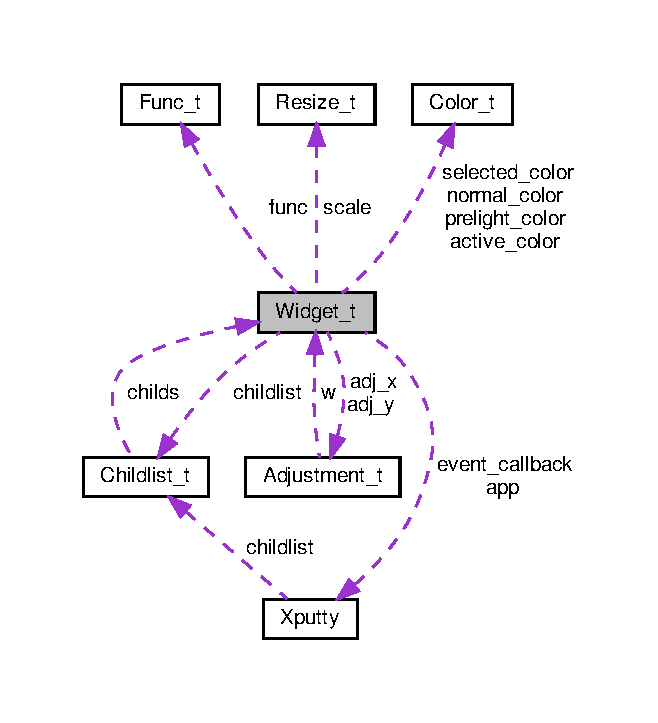
\includegraphics[width=350pt]{structWidget__t__coll__graph}
\end{center}
\end{figure}
\subsection*{Data Fields}
\begin{DoxyCompactItemize}
\item 
\hyperlink{structXputty}{Xputty} $\ast$ \hyperlink{structWidget__t_a06eaa5b134c47983fd965e745cdbaa3b}{app}
\item 
Window \hyperlink{structWidget__t_acb2bfb41674371ee1220a9d6a2d89fb1}{widget}
\item 
void $\ast$ \hyperlink{structWidget__t_a483f6517c19fe09e1bf2eaec6646a14b}{parent}
\item 
void $\ast$ \hyperlink{structWidget__t_adb548fa6377a020f0563c71382305bad}{parent\+\_\+struct}
\item 
\hyperlink{xwidget_8h_a6423c133fb634585762a77dda34befab}{vfunc} \hyperlink{structWidget__t_af0adf855c1991d11f59c5b6f9a2c526a}{event\+\_\+callback}
\item 
\hyperlink{structFunc__t}{Func\+\_\+t} \hyperlink{structWidget__t_a225b9a175e132994a5aa73b59a2911ad}{func}
\item 
cairo\+\_\+surface\+\_\+t $\ast$ \hyperlink{structWidget__t_ae9b5979742ea31817ff7d7b34a56f88d}{surface}
\item 
cairo\+\_\+t $\ast$ \hyperlink{structWidget__t_a26594f6ffabe98fc08f9207150fc9417}{cr}
\item 
cairo\+\_\+surface\+\_\+t $\ast$ \hyperlink{structWidget__t_a84d225e7b261d67daa764b47c8c62107}{buffer}
\item 
cairo\+\_\+t $\ast$ \hyperlink{structWidget__t_ad98022ee160d4c0906110868fc9e5664}{crb}
\item 
cairo\+\_\+surface\+\_\+t $\ast$ \hyperlink{structWidget__t_a4e179b5ae7494b9533c8673ec3642a55}{image}
\item 
int \hyperlink{structWidget__t_a9dd7b58be77bf31ab021aa627a73186a}{data}
\item 
long int \hyperlink{structWidget__t_ada1de5e6a955dc81fa956c9e7f2d2062}{flags}
\item 
const char $\ast$ \hyperlink{structWidget__t_a952020107ac1f6d9a37b4f978f77b61c}{label}
\item 
char \hyperlink{structWidget__t_ac5cb454301472edeb16e563ef2149dbb}{input\+\_\+label} \mbox{[}32\mbox{]}
\item 
\hyperlink{structAdjustment__t}{Adjustment\+\_\+t} $\ast$ \hyperlink{structWidget__t_aabc05e0a46c85d24483fae36127b45dd}{adj\+\_\+x}
\item 
\hyperlink{structAdjustment__t}{Adjustment\+\_\+t} $\ast$ \hyperlink{structWidget__t_abde95d3fb49faff5dd852f16810115e7}{adj\+\_\+y}
\item 
\hyperlink{structAdjustment__t}{Adjustment\+\_\+t} $\ast$ \hyperlink{structWidget__t_af3fdf65eb9a663016b91ee87a96d75a8}{adj}
\item 
\hyperlink{structChildlist__t}{Childlist\+\_\+t} $\ast$ \hyperlink{structWidget__t_ac203ccbc58958a7c205897d4aba197e9}{childlist}
\item 
X\+IC \hyperlink{structWidget__t_adafb1b98ea551ef726be6c726ac2e817}{xic}
\item 
X\+IM \hyperlink{structWidget__t_a81aa76d336043a7230844d09a92113e2}{xim}
\item 
int \hyperlink{structWidget__t_aaa935b64805fdeb78acb015c67d6638c}{state}
\item 
int \hyperlink{structWidget__t_ae2d46ffb30bb2335a043d138fa05e1a3}{pos\+\_\+x}
\item 
int \hyperlink{structWidget__t_a9b127ac6b3f017b367351ee673e063c3}{pos\+\_\+y}
\item 
int \hyperlink{structWidget__t_aac6ce7621b682bb4ce88bac9181c34a7}{x}
\item 
int \hyperlink{structWidget__t_acb9402de44e47837e1821b93fc052b38}{y}
\item 
int \hyperlink{structWidget__t_a3204c88196ed5793250b3530dd719037}{width}
\item 
int \hyperlink{structWidget__t_a1def6d2237743e75a0b84ca0c34a6834}{height}
\item 
\hyperlink{structResize__t}{Resize\+\_\+t} \hyperlink{structWidget__t_a9a2d5b53f40f5bf3914fc0694027d7ec}{scale}
\end{DoxyCompactItemize}


\subsection{Detailed Description}
\hyperlink{structWidget__t}{Widget\+\_\+t} -\/ struct to hold the basic widget info. 


\begin{DoxyParams}{Parameters}
{\em $\ast$app} & -\/ pointer to the main struct \\
\hline
{\em widget} & -\/ the X11 Window \\
\hline
{\em $\ast$parent} & -\/ pointer to the Parent Window or \hyperlink{structWidget__t}{Widget\+\_\+t} \\
\hline
{\em event\+\_\+callback} & -\/ the main X\+Event callback \\
\hline
{\em func} & -\/ struct holding the event callbacks \\
\hline
{\em $\ast$surface} & -\/ pointer to the cairo xlib surface \\
\hline
{\em $\ast$cr} & -\/ pointer to the cairo xlib surface context \\
\hline
{\em $\ast$buffer} & -\/ pointer to the cairo buffer surface \\
\hline
{\em $\ast$crb} & -\/ pointer to the cairo buffer surface context \\
\hline
{\em $\ast$image} & -\/ pointer to the cairo image surface \\
\hline
{\em data} & -\/ int to hold user data \\
\hline
{\em flags} & -\/ unsigned int to hold \hyperlink{structWidget__t}{Widget\+\_\+t} flags \\
\hline
{\em $\ast$label} & -\/ pointer to the widget label \\
\hline
{\em input\+\_\+label} & -\/ char array the widget input label \\
\hline
{\em state} & -\/ int to hold the widget state \\
\hline
{\em pos\+\_\+x} & -\/ mouse pointer x position on button press \\
\hline
{\em pos\+\_\+y} & -\/ mouse pointer y position on button press \\
\hline
{\em x} & -\/ x position of Window on Parent \\
\hline
{\em y} & -\/ y position of Window on Parent \\
\hline
{\em width} & -\/ widget width \\
\hline
{\em height} & -\/ widget height \\
\hline
{\em scale} & -\/ struct used to resize child widgets \\
\hline
{\em $\ast$adj\+\_\+x} & -\/ pointer to the x axis adjustment \\
\hline
{\em $\ast$adj\+\_\+y} & -\/ pointer to the y axis adjustment \\
\hline
{\em $\ast$adj} & -\/ pointer to the adjustment in use \\
\hline
{\em $\ast$childlist} & -\/ pointer to \hyperlink{structWidget__t}{Widget\+\_\+t} child list \\
\hline
{\em xic} & -\/ Locale and U\+TF 8 support interface \\
\hline
{\em xim} & -\/ Context to Locale and U\+TF 8 support \\
\hline
\end{DoxyParams}


\subsection{Field Documentation}
\mbox{\Hypertarget{structWidget__t_af3fdf65eb9a663016b91ee87a96d75a8}\label{structWidget__t_af3fdf65eb9a663016b91ee87a96d75a8}} 
\index{Widget\+\_\+t@{Widget\+\_\+t}!adj@{adj}}
\index{adj@{adj}!Widget\+\_\+t@{Widget\+\_\+t}}
\subsubsection{\texorpdfstring{adj}{adj}}
{\footnotesize\ttfamily \hyperlink{structAdjustment__t}{Adjustment\+\_\+t}$\ast$ Widget\+\_\+t\+::adj}

pointer to the adjustment in use \mbox{\Hypertarget{structWidget__t_aabc05e0a46c85d24483fae36127b45dd}\label{structWidget__t_aabc05e0a46c85d24483fae36127b45dd}} 
\index{Widget\+\_\+t@{Widget\+\_\+t}!adj\+\_\+x@{adj\+\_\+x}}
\index{adj\+\_\+x@{adj\+\_\+x}!Widget\+\_\+t@{Widget\+\_\+t}}
\subsubsection{\texorpdfstring{adj\+\_\+x}{adj\_x}}
{\footnotesize\ttfamily \hyperlink{structAdjustment__t}{Adjustment\+\_\+t}$\ast$ Widget\+\_\+t\+::adj\+\_\+x}

pointer to the x axis adjustment \mbox{\Hypertarget{structWidget__t_abde95d3fb49faff5dd852f16810115e7}\label{structWidget__t_abde95d3fb49faff5dd852f16810115e7}} 
\index{Widget\+\_\+t@{Widget\+\_\+t}!adj\+\_\+y@{adj\+\_\+y}}
\index{adj\+\_\+y@{adj\+\_\+y}!Widget\+\_\+t@{Widget\+\_\+t}}
\subsubsection{\texorpdfstring{adj\+\_\+y}{adj\_y}}
{\footnotesize\ttfamily \hyperlink{structAdjustment__t}{Adjustment\+\_\+t}$\ast$ Widget\+\_\+t\+::adj\+\_\+y}

pointer to the y axis adjustment \mbox{\Hypertarget{structWidget__t_a06eaa5b134c47983fd965e745cdbaa3b}\label{structWidget__t_a06eaa5b134c47983fd965e745cdbaa3b}} 
\index{Widget\+\_\+t@{Widget\+\_\+t}!app@{app}}
\index{app@{app}!Widget\+\_\+t@{Widget\+\_\+t}}
\subsubsection{\texorpdfstring{app}{app}}
{\footnotesize\ttfamily \hyperlink{structXputty}{Xputty}$\ast$ Widget\+\_\+t\+::app}

pointer to the main struct \mbox{\Hypertarget{structWidget__t_a84d225e7b261d67daa764b47c8c62107}\label{structWidget__t_a84d225e7b261d67daa764b47c8c62107}} 
\index{Widget\+\_\+t@{Widget\+\_\+t}!buffer@{buffer}}
\index{buffer@{buffer}!Widget\+\_\+t@{Widget\+\_\+t}}
\subsubsection{\texorpdfstring{buffer}{buffer}}
{\footnotesize\ttfamily cairo\+\_\+surface\+\_\+t$\ast$ Widget\+\_\+t\+::buffer}

pointer to the cairo buffer surface used for transparency \mbox{\Hypertarget{structWidget__t_ac203ccbc58958a7c205897d4aba197e9}\label{structWidget__t_ac203ccbc58958a7c205897d4aba197e9}} 
\index{Widget\+\_\+t@{Widget\+\_\+t}!childlist@{childlist}}
\index{childlist@{childlist}!Widget\+\_\+t@{Widget\+\_\+t}}
\subsubsection{\texorpdfstring{childlist}{childlist}}
{\footnotesize\ttfamily \hyperlink{structChildlist__t}{Childlist\+\_\+t}$\ast$ Widget\+\_\+t\+::childlist}

pointer to \hyperlink{structWidget__t}{Widget\+\_\+t} child list \mbox{\Hypertarget{structWidget__t_a26594f6ffabe98fc08f9207150fc9417}\label{structWidget__t_a26594f6ffabe98fc08f9207150fc9417}} 
\index{Widget\+\_\+t@{Widget\+\_\+t}!cr@{cr}}
\index{cr@{cr}!Widget\+\_\+t@{Widget\+\_\+t}}
\subsubsection{\texorpdfstring{cr}{cr}}
{\footnotesize\ttfamily cairo\+\_\+t$\ast$ Widget\+\_\+t\+::cr}

pointer to the cairo xlib surface context \mbox{\Hypertarget{structWidget__t_ad98022ee160d4c0906110868fc9e5664}\label{structWidget__t_ad98022ee160d4c0906110868fc9e5664}} 
\index{Widget\+\_\+t@{Widget\+\_\+t}!crb@{crb}}
\index{crb@{crb}!Widget\+\_\+t@{Widget\+\_\+t}}
\subsubsection{\texorpdfstring{crb}{crb}}
{\footnotesize\ttfamily cairo\+\_\+t$\ast$ Widget\+\_\+t\+::crb}

pointer to the cairo buffer surface context \mbox{\Hypertarget{structWidget__t_a9dd7b58be77bf31ab021aa627a73186a}\label{structWidget__t_a9dd7b58be77bf31ab021aa627a73186a}} 
\index{Widget\+\_\+t@{Widget\+\_\+t}!data@{data}}
\index{data@{data}!Widget\+\_\+t@{Widget\+\_\+t}}
\subsubsection{\texorpdfstring{data}{data}}
{\footnotesize\ttfamily int Widget\+\_\+t\+::data}

int to hold user data \mbox{\Hypertarget{structWidget__t_af0adf855c1991d11f59c5b6f9a2c526a}\label{structWidget__t_af0adf855c1991d11f59c5b6f9a2c526a}} 
\index{Widget\+\_\+t@{Widget\+\_\+t}!event\+\_\+callback@{event\+\_\+callback}}
\index{event\+\_\+callback@{event\+\_\+callback}!Widget\+\_\+t@{Widget\+\_\+t}}
\subsubsection{\texorpdfstring{event\+\_\+callback}{event\_callback}}
{\footnotesize\ttfamily \hyperlink{xwidget_8h_a6423c133fb634585762a77dda34befab}{vfunc} Widget\+\_\+t\+::event\+\_\+callback}

the main X\+Event callback \mbox{\Hypertarget{structWidget__t_ada1de5e6a955dc81fa956c9e7f2d2062}\label{structWidget__t_ada1de5e6a955dc81fa956c9e7f2d2062}} 
\index{Widget\+\_\+t@{Widget\+\_\+t}!flags@{flags}}
\index{flags@{flags}!Widget\+\_\+t@{Widget\+\_\+t}}
\subsubsection{\texorpdfstring{flags}{flags}}
{\footnotesize\ttfamily long int Widget\+\_\+t\+::flags}

int to hold \hyperlink{structWidget__t}{Widget\+\_\+t} flags \mbox{\Hypertarget{structWidget__t_a225b9a175e132994a5aa73b59a2911ad}\label{structWidget__t_a225b9a175e132994a5aa73b59a2911ad}} 
\index{Widget\+\_\+t@{Widget\+\_\+t}!func@{func}}
\index{func@{func}!Widget\+\_\+t@{Widget\+\_\+t}}
\subsubsection{\texorpdfstring{func}{func}}
{\footnotesize\ttfamily \hyperlink{structFunc__t}{Func\+\_\+t} Widget\+\_\+t\+::func}

struct holding the event callbacks \mbox{\Hypertarget{structWidget__t_a1def6d2237743e75a0b84ca0c34a6834}\label{structWidget__t_a1def6d2237743e75a0b84ca0c34a6834}} 
\index{Widget\+\_\+t@{Widget\+\_\+t}!height@{height}}
\index{height@{height}!Widget\+\_\+t@{Widget\+\_\+t}}
\subsubsection{\texorpdfstring{height}{height}}
{\footnotesize\ttfamily int Widget\+\_\+t\+::height}

the widget size y-\/axis \mbox{\Hypertarget{structWidget__t_a4e179b5ae7494b9533c8673ec3642a55}\label{structWidget__t_a4e179b5ae7494b9533c8673ec3642a55}} 
\index{Widget\+\_\+t@{Widget\+\_\+t}!image@{image}}
\index{image@{image}!Widget\+\_\+t@{Widget\+\_\+t}}
\subsubsection{\texorpdfstring{image}{image}}
{\footnotesize\ttfamily cairo\+\_\+surface\+\_\+t$\ast$ Widget\+\_\+t\+::image}

pointer to the cairo image surface used to load a png \mbox{\Hypertarget{structWidget__t_ac5cb454301472edeb16e563ef2149dbb}\label{structWidget__t_ac5cb454301472edeb16e563ef2149dbb}} 
\index{Widget\+\_\+t@{Widget\+\_\+t}!input\+\_\+label@{input\+\_\+label}}
\index{input\+\_\+label@{input\+\_\+label}!Widget\+\_\+t@{Widget\+\_\+t}}
\subsubsection{\texorpdfstring{input\+\_\+label}{input\_label}}
{\footnotesize\ttfamily char Widget\+\_\+t\+::input\+\_\+label\mbox{[}32\mbox{]}}

char array to hold user input \mbox{\Hypertarget{structWidget__t_a952020107ac1f6d9a37b4f978f77b61c}\label{structWidget__t_a952020107ac1f6d9a37b4f978f77b61c}} 
\index{Widget\+\_\+t@{Widget\+\_\+t}!label@{label}}
\index{label@{label}!Widget\+\_\+t@{Widget\+\_\+t}}
\subsubsection{\texorpdfstring{label}{label}}
{\footnotesize\ttfamily const char$\ast$ Widget\+\_\+t\+::label}

pointer to the widget label \mbox{\Hypertarget{structWidget__t_a483f6517c19fe09e1bf2eaec6646a14b}\label{structWidget__t_a483f6517c19fe09e1bf2eaec6646a14b}} 
\index{Widget\+\_\+t@{Widget\+\_\+t}!parent@{parent}}
\index{parent@{parent}!Widget\+\_\+t@{Widget\+\_\+t}}
\subsubsection{\texorpdfstring{parent}{parent}}
{\footnotesize\ttfamily void$\ast$ Widget\+\_\+t\+::parent}

pointer to the Parent Window or \hyperlink{structWidget__t}{Widget\+\_\+t} \mbox{\Hypertarget{structWidget__t_adb548fa6377a020f0563c71382305bad}\label{structWidget__t_adb548fa6377a020f0563c71382305bad}} 
\index{Widget\+\_\+t@{Widget\+\_\+t}!parent\+\_\+struct@{parent\+\_\+struct}}
\index{parent\+\_\+struct@{parent\+\_\+struct}!Widget\+\_\+t@{Widget\+\_\+t}}
\subsubsection{\texorpdfstring{parent\+\_\+struct}{parent\_struct}}
{\footnotesize\ttfamily void$\ast$ Widget\+\_\+t\+::parent\+\_\+struct}

pointer to the Parent struct \mbox{\Hypertarget{structWidget__t_ae2d46ffb30bb2335a043d138fa05e1a3}\label{structWidget__t_ae2d46ffb30bb2335a043d138fa05e1a3}} 
\index{Widget\+\_\+t@{Widget\+\_\+t}!pos\+\_\+x@{pos\+\_\+x}}
\index{pos\+\_\+x@{pos\+\_\+x}!Widget\+\_\+t@{Widget\+\_\+t}}
\subsubsection{\texorpdfstring{pos\+\_\+x}{pos\_x}}
{\footnotesize\ttfamily int Widget\+\_\+t\+::pos\+\_\+x}

mouse pointer x position on button press \mbox{\Hypertarget{structWidget__t_a9b127ac6b3f017b367351ee673e063c3}\label{structWidget__t_a9b127ac6b3f017b367351ee673e063c3}} 
\index{Widget\+\_\+t@{Widget\+\_\+t}!pos\+\_\+y@{pos\+\_\+y}}
\index{pos\+\_\+y@{pos\+\_\+y}!Widget\+\_\+t@{Widget\+\_\+t}}
\subsubsection{\texorpdfstring{pos\+\_\+y}{pos\_y}}
{\footnotesize\ttfamily int Widget\+\_\+t\+::pos\+\_\+y}

mouse pointer y position on button press \mbox{\Hypertarget{structWidget__t_a9a2d5b53f40f5bf3914fc0694027d7ec}\label{structWidget__t_a9a2d5b53f40f5bf3914fc0694027d7ec}} 
\index{Widget\+\_\+t@{Widget\+\_\+t}!scale@{scale}}
\index{scale@{scale}!Widget\+\_\+t@{Widget\+\_\+t}}
\subsubsection{\texorpdfstring{scale}{scale}}
{\footnotesize\ttfamily \hyperlink{structResize__t}{Resize\+\_\+t} Widget\+\_\+t\+::scale}

struct used to resize child widgets \mbox{\Hypertarget{structWidget__t_aaa935b64805fdeb78acb015c67d6638c}\label{structWidget__t_aaa935b64805fdeb78acb015c67d6638c}} 
\index{Widget\+\_\+t@{Widget\+\_\+t}!state@{state}}
\index{state@{state}!Widget\+\_\+t@{Widget\+\_\+t}}
\subsubsection{\texorpdfstring{state}{state}}
{\footnotesize\ttfamily int Widget\+\_\+t\+::state}

int to hold the widget state default = 0 \mbox{\Hypertarget{structWidget__t_ae9b5979742ea31817ff7d7b34a56f88d}\label{structWidget__t_ae9b5979742ea31817ff7d7b34a56f88d}} 
\index{Widget\+\_\+t@{Widget\+\_\+t}!surface@{surface}}
\index{surface@{surface}!Widget\+\_\+t@{Widget\+\_\+t}}
\subsubsection{\texorpdfstring{surface}{surface}}
{\footnotesize\ttfamily cairo\+\_\+surface\+\_\+t$\ast$ Widget\+\_\+t\+::surface}

pointer to the cairo xlib surface \mbox{\Hypertarget{structWidget__t_acb2bfb41674371ee1220a9d6a2d89fb1}\label{structWidget__t_acb2bfb41674371ee1220a9d6a2d89fb1}} 
\index{Widget\+\_\+t@{Widget\+\_\+t}!widget@{widget}}
\index{widget@{widget}!Widget\+\_\+t@{Widget\+\_\+t}}
\subsubsection{\texorpdfstring{widget}{widget}}
{\footnotesize\ttfamily Window Widget\+\_\+t\+::widget}

the X11 newly created Window \mbox{\Hypertarget{structWidget__t_a3204c88196ed5793250b3530dd719037}\label{structWidget__t_a3204c88196ed5793250b3530dd719037}} 
\index{Widget\+\_\+t@{Widget\+\_\+t}!width@{width}}
\index{width@{width}!Widget\+\_\+t@{Widget\+\_\+t}}
\subsubsection{\texorpdfstring{width}{width}}
{\footnotesize\ttfamily int Widget\+\_\+t\+::width}

the widget size x-\/axis \mbox{\Hypertarget{structWidget__t_aac6ce7621b682bb4ce88bac9181c34a7}\label{structWidget__t_aac6ce7621b682bb4ce88bac9181c34a7}} 
\index{Widget\+\_\+t@{Widget\+\_\+t}!x@{x}}
\index{x@{x}!Widget\+\_\+t@{Widget\+\_\+t}}
\subsubsection{\texorpdfstring{x}{x}}
{\footnotesize\ttfamily int Widget\+\_\+t\+::x}

x position of Window related to the Parent \mbox{\Hypertarget{structWidget__t_adafb1b98ea551ef726be6c726ac2e817}\label{structWidget__t_adafb1b98ea551ef726be6c726ac2e817}} 
\index{Widget\+\_\+t@{Widget\+\_\+t}!xic@{xic}}
\index{xic@{xic}!Widget\+\_\+t@{Widget\+\_\+t}}
\subsubsection{\texorpdfstring{xic}{xic}}
{\footnotesize\ttfamily X\+IC Widget\+\_\+t\+::xic}

Locale and U\+TF 8 support \mbox{\Hypertarget{structWidget__t_a81aa76d336043a7230844d09a92113e2}\label{structWidget__t_a81aa76d336043a7230844d09a92113e2}} 
\index{Widget\+\_\+t@{Widget\+\_\+t}!xim@{xim}}
\index{xim@{xim}!Widget\+\_\+t@{Widget\+\_\+t}}
\subsubsection{\texorpdfstring{xim}{xim}}
{\footnotesize\ttfamily X\+IM Widget\+\_\+t\+::xim}

Context to Locale and U\+TF 8 support \mbox{\Hypertarget{structWidget__t_acb9402de44e47837e1821b93fc052b38}\label{structWidget__t_acb9402de44e47837e1821b93fc052b38}} 
\index{Widget\+\_\+t@{Widget\+\_\+t}!y@{y}}
\index{y@{y}!Widget\+\_\+t@{Widget\+\_\+t}}
\subsubsection{\texorpdfstring{y}{y}}
{\footnotesize\ttfamily int Widget\+\_\+t\+::y}

y position of Window related to the Parent 

The documentation for this struct was generated from the following file\+:\begin{DoxyCompactItemize}
\item 
\hyperlink{xwidget_8h}{xwidget.\+h}\end{DoxyCompactItemize}

\hypertarget{structXputty}{}\section{Xputty Struct Reference}
\label{structXputty}\index{Xputty@{Xputty}}


\hyperlink{structXputty}{Xputty} -\/ the main struct. It should be declared before any other call to a \hyperlink{structXputty}{Xputty} function.  




{\ttfamily \#include $<$xputty.\+h$>$}



Collaboration diagram for Xputty\+:
\nopagebreak
\begin{figure}[H]
\begin{center}
\leavevmode
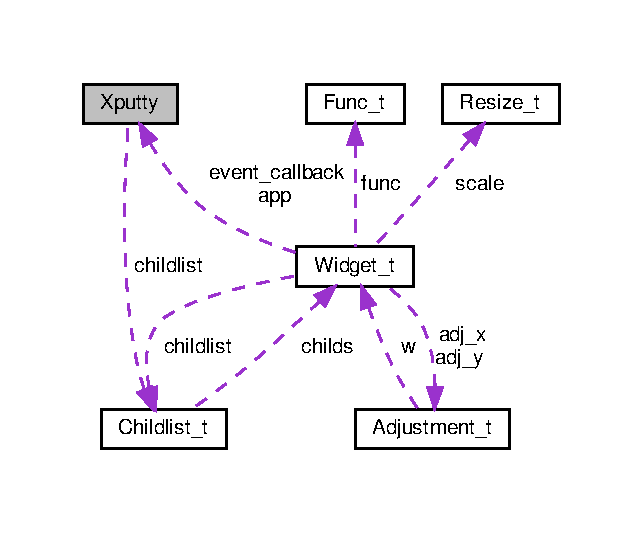
\includegraphics[width=350pt]{structXputty__coll__graph}
\end{center}
\end{figure}
\subsection*{Data Fields}
\begin{DoxyCompactItemize}
\item 
\hyperlink{structChildlist__t}{Childlist\+\_\+t} $\ast$ \hyperlink{structXputty_a55fafc08d9702ab14137f52f35c4ff19}{childlist}
\item 
Display $\ast$ \hyperlink{structXputty_ab185ae4fd00ee1930c61e0440734878f}{dpy}
\item 
bool \hyperlink{structXputty_a3a8e0381e77ae9fae69aab5dda8e7e7a}{run}
\end{DoxyCompactItemize}


\subsection{Detailed Description}
\hyperlink{structXputty}{Xputty} -\/ the main struct. It should be declared before any other call to a \hyperlink{structXputty}{Xputty} function. 


\begin{DoxyParams}{Parameters}
{\em $\ast$childlist} & -\/ pointer to the main childlist \\
\hline
{\em $\ast$dpy} & -\/ pointer to the display in use \\
\hline
{\em run} & -\/ bool to quit the main loop \\
\hline
\end{DoxyParams}


\subsection{Field Documentation}
\mbox{\Hypertarget{structXputty_a55fafc08d9702ab14137f52f35c4ff19}\label{structXputty_a55fafc08d9702ab14137f52f35c4ff19}} 
\index{Xputty@{Xputty}!childlist@{childlist}}
\index{childlist@{childlist}!Xputty@{Xputty}}
\subsubsection{\texorpdfstring{childlist}{childlist}}
{\footnotesize\ttfamily \hyperlink{structChildlist__t}{Childlist\+\_\+t}$\ast$ Xputty\+::childlist}

pointer to the main childlist \mbox{\Hypertarget{structXputty_ab185ae4fd00ee1930c61e0440734878f}\label{structXputty_ab185ae4fd00ee1930c61e0440734878f}} 
\index{Xputty@{Xputty}!dpy@{dpy}}
\index{dpy@{dpy}!Xputty@{Xputty}}
\subsubsection{\texorpdfstring{dpy}{dpy}}
{\footnotesize\ttfamily Display$\ast$ Xputty\+::dpy}

pointer to the display in use \mbox{\Hypertarget{structXputty_a3a8e0381e77ae9fae69aab5dda8e7e7a}\label{structXputty_a3a8e0381e77ae9fae69aab5dda8e7e7a}} 
\index{Xputty@{Xputty}!run@{run}}
\index{run@{run}!Xputty@{Xputty}}
\subsubsection{\texorpdfstring{run}{run}}
{\footnotesize\ttfamily bool Xputty\+::run}

bool to quit the main loop 

The documentation for this struct was generated from the following file\+:\begin{DoxyCompactItemize}
\item 
\hyperlink{xputty_8h}{xputty.\+h}\end{DoxyCompactItemize}

\chapter{File Documentation}
\hypertarget{README_8md}{}\section{R\+E\+A\+D\+M\+E.\+md File Reference}
\label{README_8md}\index{R\+E\+A\+D\+M\+E.\+md@{R\+E\+A\+D\+M\+E.\+md}}

\hypertarget{xadjustment_8c}{}\section{xadjustment.\+c File Reference}
\label{xadjustment_8c}\index{xadjustment.\+c@{xadjustment.\+c}}
{\ttfamily \#include \char`\"{}xadjustment.\+h\char`\"{}}\newline
{\ttfamily \#include \char`\"{}xadjustment\+\_\+private.\+h\char`\"{}}\newline
Include dependency graph for xadjustment.\+c\+:
\nopagebreak
\begin{figure}[H]
\begin{center}
\leavevmode
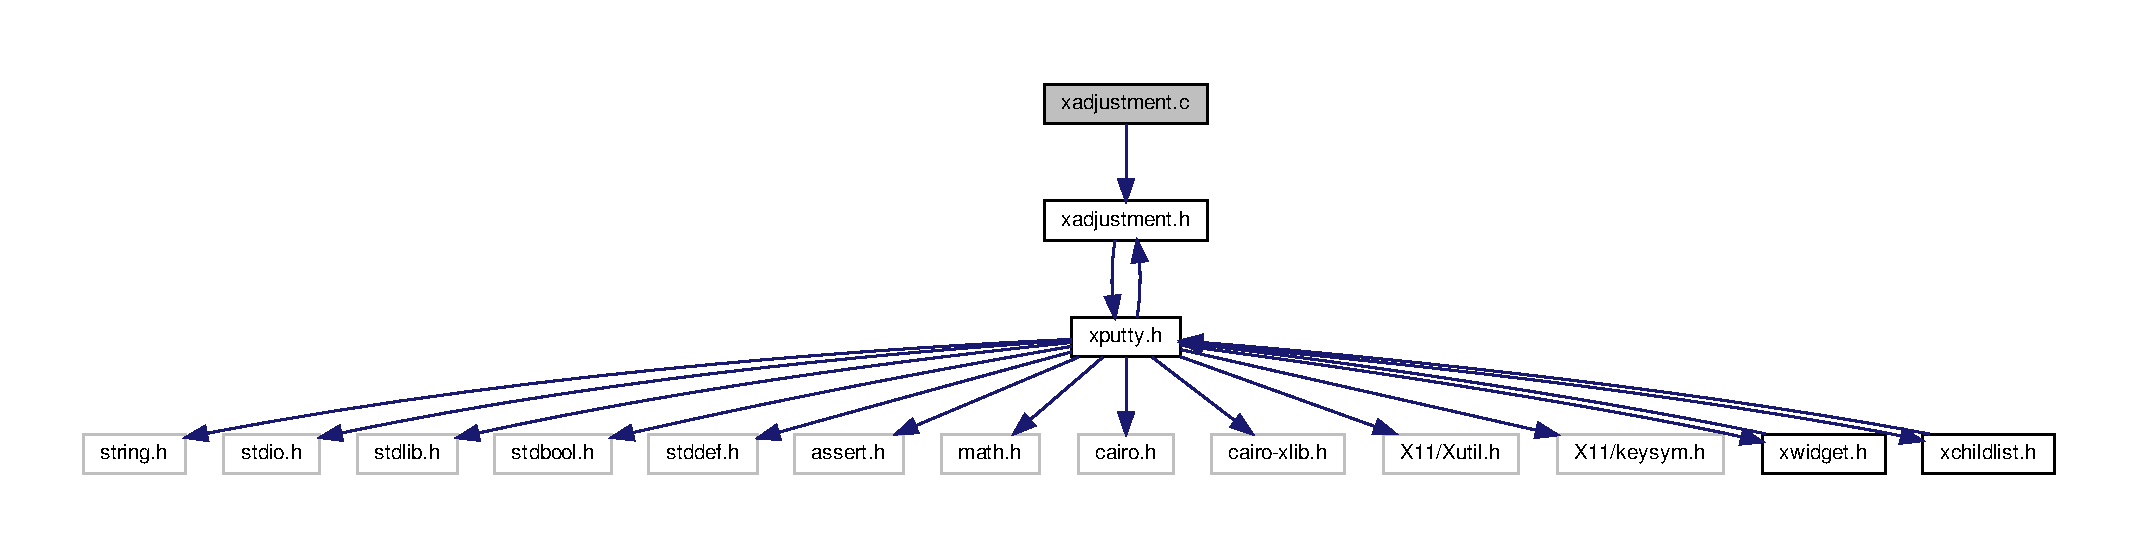
\includegraphics[width=350pt]{xadjustment_8c__incl}
\end{center}
\end{figure}
\subsection*{Functions}
\begin{DoxyCompactItemize}
\item 
\hyperlink{structAdjustment__t}{Adjustment\+\_\+t} $\ast$ \hyperlink{xadjustment_8c_afd8595365c53be47a55fecec996347a7}{add\+\_\+adjustment} (\hyperlink{structWidget__t}{Widget\+\_\+t} $\ast$w, float std\+\_\+value, float value, float min\+\_\+value, float max\+\_\+value, float step, \hyperlink{xadjustment_8h_aefe5e135b1a0eab4675337a0967a7743}{C\+L\+\_\+type} type)
\begin{DoxyCompactList}\small\item\em $\ast$add\+\_\+adjustment -\/ adding a adjustment to the widget \end{DoxyCompactList}\item 
void $\ast$ \hyperlink{xadjustment_8c_af8186d7e68d37007f6e38814225e6ee3}{delete\+\_\+adjustment} (\hyperlink{structAdjustment__t}{Adjustment\+\_\+t} $\ast$adj)
\begin{DoxyCompactList}\small\item\em delete\+\_\+adjustment -\/ freeing the memory of the adjustment \end{DoxyCompactList}\item 
float \hyperlink{xadjustment_8c_af1f74e9733cffbb287e4912fc8ab37cd}{adj\+\_\+get\+\_\+state} (\hyperlink{structAdjustment__t}{Adjustment\+\_\+t} $\ast$adj)
\begin{DoxyCompactList}\small\item\em adj\+\_\+get\+\_\+state -\/ get the current state of the adjustment \end{DoxyCompactList}\item 
float \hyperlink{xadjustment_8c_a5a78c30051a7a9c3dc0ce84c3482c530}{adj\+\_\+get\+\_\+value} (\hyperlink{structAdjustment__t}{Adjustment\+\_\+t} $\ast$adj)
\begin{DoxyCompactList}\small\item\em adj\+\_\+get\+\_\+value -\/ get the current value of the adjustment \end{DoxyCompactList}\item 
void \hyperlink{xadjustment_8c_afbe410bb3efb6e78941a4f938d1c67ca}{adj\+\_\+set\+\_\+value} (\hyperlink{structAdjustment__t}{Adjustment\+\_\+t} $\ast$adj, float v)
\begin{DoxyCompactList}\small\item\em adj\+\_\+set\+\_\+value -\/ set the current value of the adjustment \end{DoxyCompactList}\item 
void \hyperlink{xadjustment_8c_a670e06d916d1d6fd1f2968fb171c29aa}{adj\+\_\+set\+\_\+start\+\_\+value} (void $\ast$w)
\begin{DoxyCompactList}\small\item\em adj\+\_\+set\+\_\+start\+\_\+value -\/ set start value of the adjustment \end{DoxyCompactList}\item 
void \hyperlink{xadjustment_8c_aaeeb13f45a95f6e2f585641b212eca11}{adj\+\_\+set\+\_\+state} (void $\ast$w, float x, float y)
\begin{DoxyCompactList}\small\item\em adj\+\_\+set\+\_\+state -\/ set value/state of the adjustment \end{DoxyCompactList}\end{DoxyCompactItemize}


\subsection{Function Documentation}
\mbox{\Hypertarget{xadjustment_8c_afd8595365c53be47a55fecec996347a7}\label{xadjustment_8c_afd8595365c53be47a55fecec996347a7}} 
\index{xadjustment.\+c@{xadjustment.\+c}!add\+\_\+adjustment@{add\+\_\+adjustment}}
\index{add\+\_\+adjustment@{add\+\_\+adjustment}!xadjustment.\+c@{xadjustment.\+c}}
\subsubsection{\texorpdfstring{add\+\_\+adjustment()}{add\_adjustment()}}
{\footnotesize\ttfamily \hyperlink{structAdjustment__t}{Adjustment\+\_\+t}$\ast$ add\+\_\+adjustment (\begin{DoxyParamCaption}\item[{\hyperlink{structWidget__t}{Widget\+\_\+t} $\ast$}]{w,  }\item[{float}]{std\+\_\+value,  }\item[{float}]{value,  }\item[{float}]{min\+\_\+value,  }\item[{float}]{max\+\_\+value,  }\item[{float}]{step,  }\item[{\hyperlink{xadjustment_8h_aefe5e135b1a0eab4675337a0967a7743}{C\+L\+\_\+type}}]{type }\end{DoxyParamCaption})}



$\ast$add\+\_\+adjustment -\/ adding a adjustment to the widget 


\begin{DoxyParams}{Parameters}
{\em $\ast$w} & -\/ pointer to the \hyperlink{structWidget__t}{Widget\+\_\+t} request a adjustment \\
\hline
{\em std\+\_\+value} & -\/ standard value of the adjustment \\
\hline
{\em value} & -\/ current value of the adjustment \\
\hline
{\em min\+\_\+value} & -\/ minimum value of the adjustment \\
\hline
{\em max\+\_\+value} & -\/ maximal value of the adjustment \\
\hline
{\em step} & -\/ step to increase/decrease the adjustment \\
\hline
{\em type} & -\/ set C\+L\+\_\+type of adjustment \\
\hline
\end{DoxyParams}
\begin{DoxyReturn}{Returns}
$\ast$adj -\/ pointer to adjustment 
\end{DoxyReturn}
\mbox{\Hypertarget{xadjustment_8c_af1f74e9733cffbb287e4912fc8ab37cd}\label{xadjustment_8c_af1f74e9733cffbb287e4912fc8ab37cd}} 
\index{xadjustment.\+c@{xadjustment.\+c}!adj\+\_\+get\+\_\+state@{adj\+\_\+get\+\_\+state}}
\index{adj\+\_\+get\+\_\+state@{adj\+\_\+get\+\_\+state}!xadjustment.\+c@{xadjustment.\+c}}
\subsubsection{\texorpdfstring{adj\+\_\+get\+\_\+state()}{adj\_get\_state()}}
{\footnotesize\ttfamily float adj\+\_\+get\+\_\+state (\begin{DoxyParamCaption}\item[{\hyperlink{structAdjustment__t}{Adjustment\+\_\+t} $\ast$}]{adj }\end{DoxyParamCaption})}



adj\+\_\+get\+\_\+state -\/ get the current state of the adjustment 


\begin{DoxyParams}{Parameters}
{\em $\ast$adj} & -\/ pointer to the Adjustment to free \\
\hline
\end{DoxyParams}
\begin{DoxyReturn}{Returns}
float -\/ return the adjustment state (0$<$-\/$>$1) 
\end{DoxyReturn}
\mbox{\Hypertarget{xadjustment_8c_a5a78c30051a7a9c3dc0ce84c3482c530}\label{xadjustment_8c_a5a78c30051a7a9c3dc0ce84c3482c530}} 
\index{xadjustment.\+c@{xadjustment.\+c}!adj\+\_\+get\+\_\+value@{adj\+\_\+get\+\_\+value}}
\index{adj\+\_\+get\+\_\+value@{adj\+\_\+get\+\_\+value}!xadjustment.\+c@{xadjustment.\+c}}
\subsubsection{\texorpdfstring{adj\+\_\+get\+\_\+value()}{adj\_get\_value()}}
{\footnotesize\ttfamily float adj\+\_\+get\+\_\+value (\begin{DoxyParamCaption}\item[{\hyperlink{structAdjustment__t}{Adjustment\+\_\+t} $\ast$}]{adj }\end{DoxyParamCaption})}



adj\+\_\+get\+\_\+value -\/ get the current value of the adjustment 


\begin{DoxyParams}{Parameters}
{\em $\ast$adj} & -\/ pointer to the Adjustment to free \\
\hline
\end{DoxyParams}
\begin{DoxyReturn}{Returns}
float -\/ return the adjustment value 
\end{DoxyReturn}
\mbox{\Hypertarget{xadjustment_8c_a670e06d916d1d6fd1f2968fb171c29aa}\label{xadjustment_8c_a670e06d916d1d6fd1f2968fb171c29aa}} 
\index{xadjustment.\+c@{xadjustment.\+c}!adj\+\_\+set\+\_\+start\+\_\+value@{adj\+\_\+set\+\_\+start\+\_\+value}}
\index{adj\+\_\+set\+\_\+start\+\_\+value@{adj\+\_\+set\+\_\+start\+\_\+value}!xadjustment.\+c@{xadjustment.\+c}}
\subsubsection{\texorpdfstring{adj\+\_\+set\+\_\+start\+\_\+value()}{adj\_set\_start\_value()}}
{\footnotesize\ttfamily void adj\+\_\+set\+\_\+start\+\_\+value (\begin{DoxyParamCaption}\item[{void $\ast$}]{w }\end{DoxyParamCaption})}



adj\+\_\+set\+\_\+start\+\_\+value -\/ set start value of the adjustment 


\begin{DoxyParams}{Parameters}
{\em $\ast$w} & -\/ pointer to \hyperlink{structWidget__t}{Widget\+\_\+t} containing the adjustment \\
\hline
\end{DoxyParams}
\begin{DoxyReturn}{Returns}
void 
\end{DoxyReturn}
\mbox{\Hypertarget{xadjustment_8c_aaeeb13f45a95f6e2f585641b212eca11}\label{xadjustment_8c_aaeeb13f45a95f6e2f585641b212eca11}} 
\index{xadjustment.\+c@{xadjustment.\+c}!adj\+\_\+set\+\_\+state@{adj\+\_\+set\+\_\+state}}
\index{adj\+\_\+set\+\_\+state@{adj\+\_\+set\+\_\+state}!xadjustment.\+c@{xadjustment.\+c}}
\subsubsection{\texorpdfstring{adj\+\_\+set\+\_\+state()}{adj\_set\_state()}}
{\footnotesize\ttfamily void adj\+\_\+set\+\_\+state (\begin{DoxyParamCaption}\item[{void $\ast$}]{w,  }\item[{float}]{x,  }\item[{float}]{y }\end{DoxyParamCaption})}



adj\+\_\+set\+\_\+state -\/ set value/state of the adjustment 


\begin{DoxyParams}{Parameters}
{\em $\ast$adj} & -\/ pointer to \hyperlink{structWidget__t}{Widget\+\_\+t} containing the adjustment \\
\hline
{\em x} & -\/ value for the xaxis \\
\hline
{\em y} & -\/ value for the yaxis \\
\hline
\end{DoxyParams}
\begin{DoxyReturn}{Returns}
void 
\end{DoxyReturn}
\mbox{\Hypertarget{xadjustment_8c_afbe410bb3efb6e78941a4f938d1c67ca}\label{xadjustment_8c_afbe410bb3efb6e78941a4f938d1c67ca}} 
\index{xadjustment.\+c@{xadjustment.\+c}!adj\+\_\+set\+\_\+value@{adj\+\_\+set\+\_\+value}}
\index{adj\+\_\+set\+\_\+value@{adj\+\_\+set\+\_\+value}!xadjustment.\+c@{xadjustment.\+c}}
\subsubsection{\texorpdfstring{adj\+\_\+set\+\_\+value()}{adj\_set\_value()}}
{\footnotesize\ttfamily void adj\+\_\+set\+\_\+value (\begin{DoxyParamCaption}\item[{\hyperlink{structAdjustment__t}{Adjustment\+\_\+t} $\ast$}]{adj,  }\item[{float}]{v }\end{DoxyParamCaption})}



adj\+\_\+set\+\_\+value -\/ set the current value of the adjustment 


\begin{DoxyParams}{Parameters}
{\em $\ast$adj} & -\/ pointer to the Adjustment to free \\
\hline
{\em v} & -\/ value set the Adjustment to \\
\hline
\end{DoxyParams}
\begin{DoxyReturn}{Returns}
void 
\end{DoxyReturn}
\mbox{\Hypertarget{xadjustment_8c_af8186d7e68d37007f6e38814225e6ee3}\label{xadjustment_8c_af8186d7e68d37007f6e38814225e6ee3}} 
\index{xadjustment.\+c@{xadjustment.\+c}!delete\+\_\+adjustment@{delete\+\_\+adjustment}}
\index{delete\+\_\+adjustment@{delete\+\_\+adjustment}!xadjustment.\+c@{xadjustment.\+c}}
\subsubsection{\texorpdfstring{delete\+\_\+adjustment()}{delete\_adjustment()}}
{\footnotesize\ttfamily void$\ast$ delete\+\_\+adjustment (\begin{DoxyParamCaption}\item[{\hyperlink{structAdjustment__t}{Adjustment\+\_\+t} $\ast$}]{adj }\end{DoxyParamCaption})}



delete\+\_\+adjustment -\/ freeing the memory of the adjustment 


\begin{DoxyParams}{Parameters}
{\em $\ast$adj} & -\/ pointer to the Adjustment to free \\
\hline
\end{DoxyParams}
\begin{DoxyReturn}{Returns}
$\ast$void -\/ return N\+U\+LL 
\end{DoxyReturn}

\hypertarget{xadjustment_8h}{}\section{xadjustment.\+h File Reference}
\label{xadjustment_8h}\index{xadjustment.\+h@{xadjustment.\+h}}
{\ttfamily \#include \char`\"{}xputty.\+h\char`\"{}}\newline
Include dependency graph for xadjustment.\+h\+:
\nopagebreak
\begin{figure}[H]
\begin{center}
\leavevmode
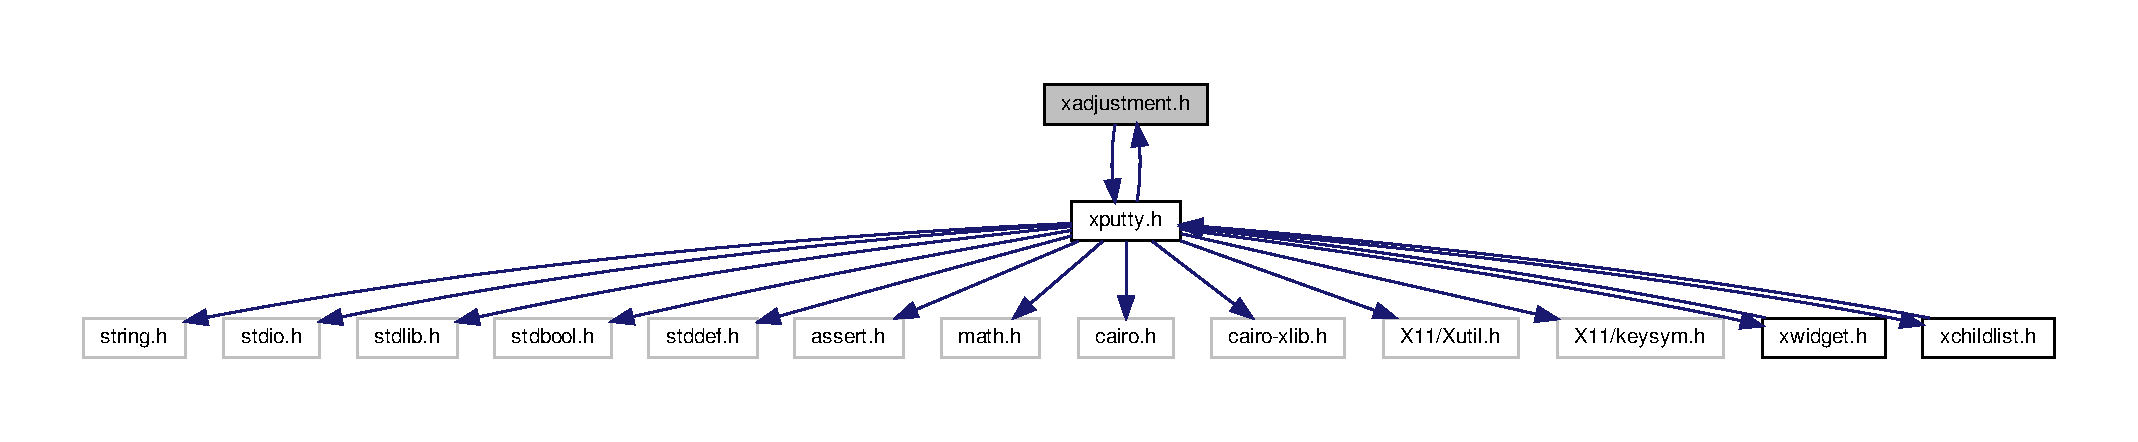
\includegraphics[width=350pt]{xadjustment_8h__incl}
\end{center}
\end{figure}
This graph shows which files directly or indirectly include this file\+:
\nopagebreak
\begin{figure}[H]
\begin{center}
\leavevmode
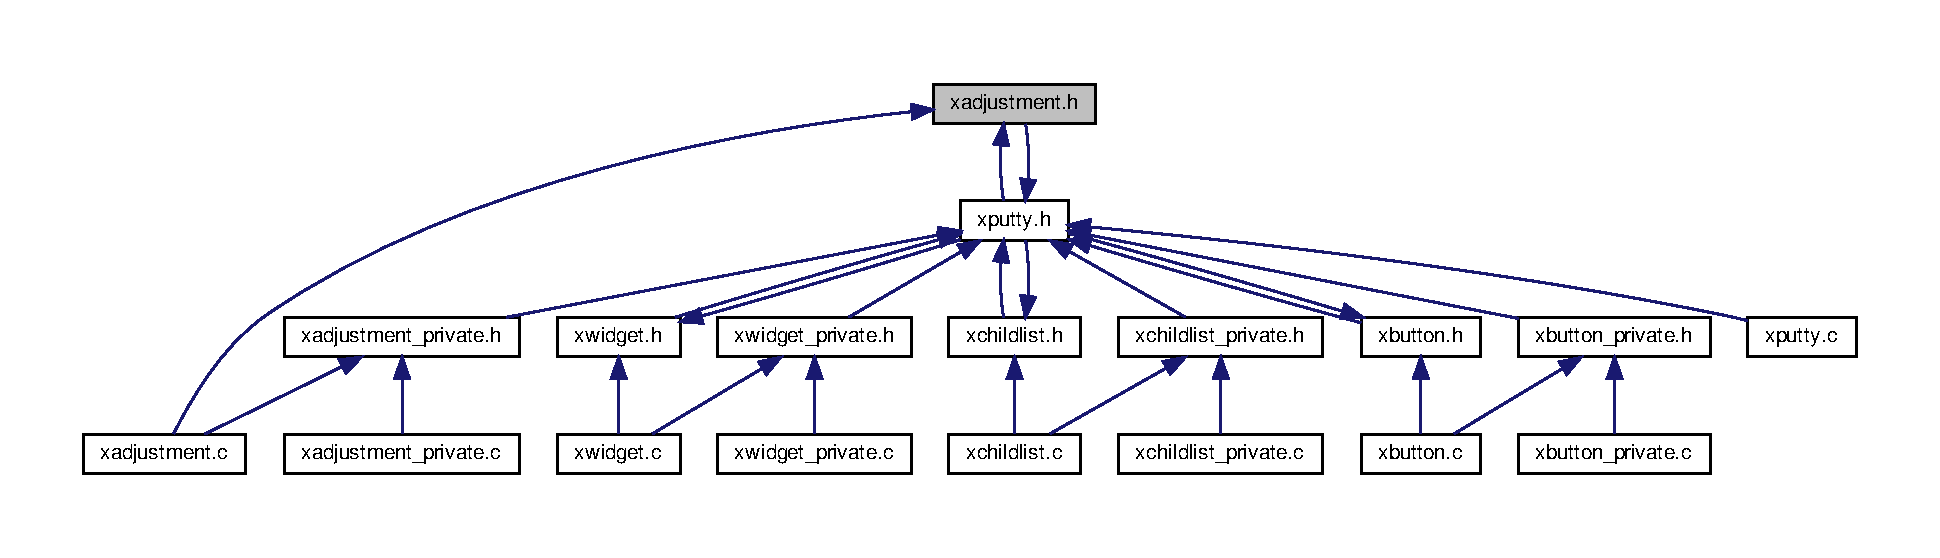
\includegraphics[width=350pt]{xadjustment_8h__dep__incl}
\end{center}
\end{figure}
\subsection*{Data Structures}
\begin{DoxyCompactItemize}
\item 
struct \hyperlink{structAdjustment__t}{Adjustment\+\_\+t}
\begin{DoxyCompactList}\small\item\em \hyperlink{structAdjustment__t}{Adjustment\+\_\+t} -\/ struct to hold a controller adjustment. \end{DoxyCompactList}\end{DoxyCompactItemize}
\subsection*{Macros}
\begin{DoxyCompactItemize}
\item 
\#define \hyperlink{xadjustment_8h_a32f69912c546bd28e73b2f48cc99a99d}{X\+A\+D\+J\+U\+S\+T\+M\+E\+N\+T\+\_\+\+H\+\_\+}
\end{DoxyCompactItemize}
\subsection*{Enumerations}
\begin{DoxyCompactItemize}
\item 
enum \hyperlink{xadjustment_8h_aefe5e135b1a0eab4675337a0967a7743}{C\+L\+\_\+type} \{ \newline
\hyperlink{xadjustment_8h_aefe5e135b1a0eab4675337a0967a7743a6dc58bda20e0018d54f1cb94df78119e}{C\+L\+\_\+\+N\+O\+NE} = 0x0001, 
\hyperlink{xadjustment_8h_aefe5e135b1a0eab4675337a0967a7743a62a789a6ef19826f17aefdceba303647}{C\+L\+\_\+\+C\+O\+N\+T\+I\+N\+U\+OS} = 0x0002, 
\hyperlink{xadjustment_8h_aefe5e135b1a0eab4675337a0967a7743a08e7c21e78e2617f5f20de6b919b0e6c}{C\+L\+\_\+\+T\+O\+G\+G\+LE} = 0x0004, 
\hyperlink{xadjustment_8h_aefe5e135b1a0eab4675337a0967a7743abc74a250346d4b52e2fa55dbf4da1ef0}{C\+L\+\_\+\+B\+U\+T\+T\+ON} = 0x0008, 
\newline
\hyperlink{xadjustment_8h_aefe5e135b1a0eab4675337a0967a7743a86ad020137af474591a13badc9e3bf78}{C\+L\+\_\+\+E\+N\+UM} = 0x0010
 \}\begin{DoxyCompactList}\small\item\em C\+L\+\_\+type -\/ enum type of controller adjustment. \end{DoxyCompactList}
\end{DoxyCompactItemize}
\subsection*{Functions}
\begin{DoxyCompactItemize}
\item 
\hyperlink{structAdjustment__t}{Adjustment\+\_\+t} $\ast$ \hyperlink{xadjustment_8h_afd8595365c53be47a55fecec996347a7}{add\+\_\+adjustment} (\hyperlink{structWidget__t}{Widget\+\_\+t} $\ast$w, float std\+\_\+value, float value, float min\+\_\+value, float max\+\_\+value, float step, \hyperlink{xadjustment_8h_aefe5e135b1a0eab4675337a0967a7743}{C\+L\+\_\+type} type)
\begin{DoxyCompactList}\small\item\em $\ast$add\+\_\+adjustment -\/ adding a adjustment to the widget \end{DoxyCompactList}\item 
void \hyperlink{xadjustment_8h_ab7188a4bb4294e2a08aea2430975b406}{set\+\_\+adjustment} (\hyperlink{structAdjustment__t}{Adjustment\+\_\+t} $\ast$adj, float std\+\_\+value, float value, float min\+\_\+value, float max\+\_\+value, float step, \hyperlink{xadjustment_8h_aefe5e135b1a0eab4675337a0967a7743}{C\+L\+\_\+type} type)
\begin{DoxyCompactList}\small\item\em $\ast$set\+\_\+adjustment -\/ set a new range to a existing Adjustment \end{DoxyCompactList}\item 
void $\ast$ \hyperlink{xadjustment_8h_af8186d7e68d37007f6e38814225e6ee3}{delete\+\_\+adjustment} (\hyperlink{structAdjustment__t}{Adjustment\+\_\+t} $\ast$adj)
\begin{DoxyCompactList}\small\item\em delete\+\_\+adjustment -\/ freeing the memory of the adjustment \end{DoxyCompactList}\item 
float \hyperlink{xadjustment_8h_af1f74e9733cffbb287e4912fc8ab37cd}{adj\+\_\+get\+\_\+state} (\hyperlink{structAdjustment__t}{Adjustment\+\_\+t} $\ast$adj)
\begin{DoxyCompactList}\small\item\em adj\+\_\+get\+\_\+state -\/ get the current state of the adjustment \end{DoxyCompactList}\item 
float \hyperlink{xadjustment_8h_a5a78c30051a7a9c3dc0ce84c3482c530}{adj\+\_\+get\+\_\+value} (\hyperlink{structAdjustment__t}{Adjustment\+\_\+t} $\ast$adj)
\begin{DoxyCompactList}\small\item\em adj\+\_\+get\+\_\+value -\/ get the current value of the adjustment \end{DoxyCompactList}\item 
void \hyperlink{xadjustment_8h_afbe410bb3efb6e78941a4f938d1c67ca}{adj\+\_\+set\+\_\+value} (\hyperlink{structAdjustment__t}{Adjustment\+\_\+t} $\ast$adj, float v)
\begin{DoxyCompactList}\small\item\em adj\+\_\+set\+\_\+value -\/ set the current value of the adjustment \end{DoxyCompactList}\item 
void \hyperlink{xadjustment_8h_a670e06d916d1d6fd1f2968fb171c29aa}{adj\+\_\+set\+\_\+start\+\_\+value} (void $\ast$w)
\begin{DoxyCompactList}\small\item\em adj\+\_\+set\+\_\+start\+\_\+value -\/ set start value of the adjustment \end{DoxyCompactList}\item 
void \hyperlink{xadjustment_8h_aaeeb13f45a95f6e2f585641b212eca11}{adj\+\_\+set\+\_\+state} (void $\ast$w, float x, float y)
\begin{DoxyCompactList}\small\item\em adj\+\_\+set\+\_\+state -\/ set value/state of the adjustment \end{DoxyCompactList}\item 
void \hyperlink{xadjustment_8h_a1db458f5dc9ea4f3775340b938b3c3bf}{check\+\_\+value\+\_\+changed} (\hyperlink{structAdjustment__t}{Adjustment\+\_\+t} $\ast$adj, float $\ast$value)
\begin{DoxyCompactList}\small\item\em check\+\_\+value\+\_\+changed -\/ check if value has changed and send adj\+\_\+callback if so \end{DoxyCompactList}\end{DoxyCompactItemize}


\subsection{Macro Definition Documentation}
\mbox{\Hypertarget{xadjustment_8h_a32f69912c546bd28e73b2f48cc99a99d}\label{xadjustment_8h_a32f69912c546bd28e73b2f48cc99a99d}} 
\index{xadjustment.\+h@{xadjustment.\+h}!X\+A\+D\+J\+U\+S\+T\+M\+E\+N\+T\+\_\+\+H\+\_\+@{X\+A\+D\+J\+U\+S\+T\+M\+E\+N\+T\+\_\+\+H\+\_\+}}
\index{X\+A\+D\+J\+U\+S\+T\+M\+E\+N\+T\+\_\+\+H\+\_\+@{X\+A\+D\+J\+U\+S\+T\+M\+E\+N\+T\+\_\+\+H\+\_\+}!xadjustment.\+h@{xadjustment.\+h}}
\subsubsection{\texorpdfstring{X\+A\+D\+J\+U\+S\+T\+M\+E\+N\+T\+\_\+\+H\+\_\+}{XADJUSTMENT\_H\_}}
{\footnotesize\ttfamily \#define X\+A\+D\+J\+U\+S\+T\+M\+E\+N\+T\+\_\+\+H\+\_\+}



\subsection{Enumeration Type Documentation}
\mbox{\Hypertarget{xadjustment_8h_aefe5e135b1a0eab4675337a0967a7743}\label{xadjustment_8h_aefe5e135b1a0eab4675337a0967a7743}} 
\index{xadjustment.\+h@{xadjustment.\+h}!C\+L\+\_\+type@{C\+L\+\_\+type}}
\index{C\+L\+\_\+type@{C\+L\+\_\+type}!xadjustment.\+h@{xadjustment.\+h}}
\subsubsection{\texorpdfstring{C\+L\+\_\+type}{CL\_type}}
{\footnotesize\ttfamily enum \hyperlink{xadjustment_8h_aefe5e135b1a0eab4675337a0967a7743}{C\+L\+\_\+type}}



C\+L\+\_\+type -\/ enum type of controller adjustment. 


\begin{DoxyParams}{Parameters}
{\em C\+L\+\_\+\+N\+O\+NE} & -\/ \hyperlink{structWidget__t}{Widget\+\_\+t} didn\textquotesingle{}t request a adjustment \\
\hline
{\em C\+L\+\_\+\+C\+O\+N\+T\+I\+N\+U\+OS} & -\/ \hyperlink{structWidget__t}{Widget\+\_\+t} request a continuos adjustment \\
\hline
{\em C\+L\+\_\+\+T\+O\+G\+G\+LE} & -\/ \hyperlink{structWidget__t}{Widget\+\_\+t} request a toggle adjustment \\
\hline
{\em C\+L\+\_\+\+B\+U\+T\+T\+ON} & -\/ \hyperlink{structWidget__t}{Widget\+\_\+t} request a button adjustment \\
\hline
{\em C\+L\+\_\+\+E\+N\+UM} & -\/ \hyperlink{structWidget__t}{Widget\+\_\+t} request a enum adjustment \\
\hline
\end{DoxyParams}
\begin{DoxyEnumFields}{Enumerator}
\raisebox{\heightof{T}}[0pt][0pt]{\index{C\+L\+\_\+\+N\+O\+NE@{C\+L\+\_\+\+N\+O\+NE}!xadjustment.\+h@{xadjustment.\+h}}\index{xadjustment.\+h@{xadjustment.\+h}!C\+L\+\_\+\+N\+O\+NE@{C\+L\+\_\+\+N\+O\+NE}}}\mbox{\Hypertarget{xadjustment_8h_aefe5e135b1a0eab4675337a0967a7743a6dc58bda20e0018d54f1cb94df78119e}\label{xadjustment_8h_aefe5e135b1a0eab4675337a0967a7743a6dc58bda20e0018d54f1cb94df78119e}} 
C\+L\+\_\+\+N\+O\+NE&\hyperlink{structWidget__t}{Widget\+\_\+t} didn\textquotesingle{}t request a adjustment \\
\hline

\raisebox{\heightof{T}}[0pt][0pt]{\index{C\+L\+\_\+\+C\+O\+N\+T\+I\+N\+U\+OS@{C\+L\+\_\+\+C\+O\+N\+T\+I\+N\+U\+OS}!xadjustment.\+h@{xadjustment.\+h}}\index{xadjustment.\+h@{xadjustment.\+h}!C\+L\+\_\+\+C\+O\+N\+T\+I\+N\+U\+OS@{C\+L\+\_\+\+C\+O\+N\+T\+I\+N\+U\+OS}}}\mbox{\Hypertarget{xadjustment_8h_aefe5e135b1a0eab4675337a0967a7743a62a789a6ef19826f17aefdceba303647}\label{xadjustment_8h_aefe5e135b1a0eab4675337a0967a7743a62a789a6ef19826f17aefdceba303647}} 
C\+L\+\_\+\+C\+O\+N\+T\+I\+N\+U\+OS&\hyperlink{structWidget__t}{Widget\+\_\+t} request a continuos adjustment \\
\hline

\raisebox{\heightof{T}}[0pt][0pt]{\index{C\+L\+\_\+\+T\+O\+G\+G\+LE@{C\+L\+\_\+\+T\+O\+G\+G\+LE}!xadjustment.\+h@{xadjustment.\+h}}\index{xadjustment.\+h@{xadjustment.\+h}!C\+L\+\_\+\+T\+O\+G\+G\+LE@{C\+L\+\_\+\+T\+O\+G\+G\+LE}}}\mbox{\Hypertarget{xadjustment_8h_aefe5e135b1a0eab4675337a0967a7743a08e7c21e78e2617f5f20de6b919b0e6c}\label{xadjustment_8h_aefe5e135b1a0eab4675337a0967a7743a08e7c21e78e2617f5f20de6b919b0e6c}} 
C\+L\+\_\+\+T\+O\+G\+G\+LE&\hyperlink{structWidget__t}{Widget\+\_\+t} request a toggle adjustment \\
\hline

\raisebox{\heightof{T}}[0pt][0pt]{\index{C\+L\+\_\+\+B\+U\+T\+T\+ON@{C\+L\+\_\+\+B\+U\+T\+T\+ON}!xadjustment.\+h@{xadjustment.\+h}}\index{xadjustment.\+h@{xadjustment.\+h}!C\+L\+\_\+\+B\+U\+T\+T\+ON@{C\+L\+\_\+\+B\+U\+T\+T\+ON}}}\mbox{\Hypertarget{xadjustment_8h_aefe5e135b1a0eab4675337a0967a7743abc74a250346d4b52e2fa55dbf4da1ef0}\label{xadjustment_8h_aefe5e135b1a0eab4675337a0967a7743abc74a250346d4b52e2fa55dbf4da1ef0}} 
C\+L\+\_\+\+B\+U\+T\+T\+ON&\hyperlink{structWidget__t}{Widget\+\_\+t} request a button adjustment \\
\hline

\raisebox{\heightof{T}}[0pt][0pt]{\index{C\+L\+\_\+\+E\+N\+UM@{C\+L\+\_\+\+E\+N\+UM}!xadjustment.\+h@{xadjustment.\+h}}\index{xadjustment.\+h@{xadjustment.\+h}!C\+L\+\_\+\+E\+N\+UM@{C\+L\+\_\+\+E\+N\+UM}}}\mbox{\Hypertarget{xadjustment_8h_aefe5e135b1a0eab4675337a0967a7743a86ad020137af474591a13badc9e3bf78}\label{xadjustment_8h_aefe5e135b1a0eab4675337a0967a7743a86ad020137af474591a13badc9e3bf78}} 
C\+L\+\_\+\+E\+N\+UM&\hyperlink{structWidget__t}{Widget\+\_\+t} request a enum adjustment \\
\hline

\end{DoxyEnumFields}


\subsection{Function Documentation}
\mbox{\Hypertarget{xadjustment_8h_afd8595365c53be47a55fecec996347a7}\label{xadjustment_8h_afd8595365c53be47a55fecec996347a7}} 
\index{xadjustment.\+h@{xadjustment.\+h}!add\+\_\+adjustment@{add\+\_\+adjustment}}
\index{add\+\_\+adjustment@{add\+\_\+adjustment}!xadjustment.\+h@{xadjustment.\+h}}
\subsubsection{\texorpdfstring{add\+\_\+adjustment()}{add\_adjustment()}}
{\footnotesize\ttfamily \hyperlink{structAdjustment__t}{Adjustment\+\_\+t}$\ast$ add\+\_\+adjustment (\begin{DoxyParamCaption}\item[{\hyperlink{structWidget__t}{Widget\+\_\+t} $\ast$}]{w,  }\item[{float}]{std\+\_\+value,  }\item[{float}]{value,  }\item[{float}]{min\+\_\+value,  }\item[{float}]{max\+\_\+value,  }\item[{float}]{step,  }\item[{\hyperlink{xadjustment_8h_aefe5e135b1a0eab4675337a0967a7743}{C\+L\+\_\+type}}]{type }\end{DoxyParamCaption})}



$\ast$add\+\_\+adjustment -\/ adding a adjustment to the widget 


\begin{DoxyParams}{Parameters}
{\em $\ast$w} & -\/ pointer to the \hyperlink{structWidget__t}{Widget\+\_\+t} request a adjustment \\
\hline
{\em std\+\_\+value} & -\/ standard value of the adjustment \\
\hline
{\em value} & -\/ current value of the adjustment \\
\hline
{\em min\+\_\+value} & -\/ minimum value of the adjustment \\
\hline
{\em max\+\_\+value} & -\/ maximal value of the adjustment \\
\hline
{\em step} & -\/ step to increase/decrease the adjustment \\
\hline
{\em type} & -\/ set C\+L\+\_\+type of adjustment \\
\hline
\end{DoxyParams}
\begin{DoxyReturn}{Returns}
$\ast$adj -\/ pointer to adjustment 
\end{DoxyReturn}
\mbox{\Hypertarget{xadjustment_8h_af1f74e9733cffbb287e4912fc8ab37cd}\label{xadjustment_8h_af1f74e9733cffbb287e4912fc8ab37cd}} 
\index{xadjustment.\+h@{xadjustment.\+h}!adj\+\_\+get\+\_\+state@{adj\+\_\+get\+\_\+state}}
\index{adj\+\_\+get\+\_\+state@{adj\+\_\+get\+\_\+state}!xadjustment.\+h@{xadjustment.\+h}}
\subsubsection{\texorpdfstring{adj\+\_\+get\+\_\+state()}{adj\_get\_state()}}
{\footnotesize\ttfamily float adj\+\_\+get\+\_\+state (\begin{DoxyParamCaption}\item[{\hyperlink{structAdjustment__t}{Adjustment\+\_\+t} $\ast$}]{adj }\end{DoxyParamCaption})}



adj\+\_\+get\+\_\+state -\/ get the current state of the adjustment 


\begin{DoxyParams}{Parameters}
{\em $\ast$adj} & -\/ pointer to the Adjustment to free \\
\hline
\end{DoxyParams}
\begin{DoxyReturn}{Returns}
float -\/ return the adjustment state (0$<$-\/$>$1) 
\end{DoxyReturn}
\mbox{\Hypertarget{xadjustment_8h_a5a78c30051a7a9c3dc0ce84c3482c530}\label{xadjustment_8h_a5a78c30051a7a9c3dc0ce84c3482c530}} 
\index{xadjustment.\+h@{xadjustment.\+h}!adj\+\_\+get\+\_\+value@{adj\+\_\+get\+\_\+value}}
\index{adj\+\_\+get\+\_\+value@{adj\+\_\+get\+\_\+value}!xadjustment.\+h@{xadjustment.\+h}}
\subsubsection{\texorpdfstring{adj\+\_\+get\+\_\+value()}{adj\_get\_value()}}
{\footnotesize\ttfamily float adj\+\_\+get\+\_\+value (\begin{DoxyParamCaption}\item[{\hyperlink{structAdjustment__t}{Adjustment\+\_\+t} $\ast$}]{adj }\end{DoxyParamCaption})}



adj\+\_\+get\+\_\+value -\/ get the current value of the adjustment 


\begin{DoxyParams}{Parameters}
{\em $\ast$adj} & -\/ pointer to the Adjustment to free \\
\hline
\end{DoxyParams}
\begin{DoxyReturn}{Returns}
float -\/ return the adjustment value 
\end{DoxyReturn}
\mbox{\Hypertarget{xadjustment_8h_a670e06d916d1d6fd1f2968fb171c29aa}\label{xadjustment_8h_a670e06d916d1d6fd1f2968fb171c29aa}} 
\index{xadjustment.\+h@{xadjustment.\+h}!adj\+\_\+set\+\_\+start\+\_\+value@{adj\+\_\+set\+\_\+start\+\_\+value}}
\index{adj\+\_\+set\+\_\+start\+\_\+value@{adj\+\_\+set\+\_\+start\+\_\+value}!xadjustment.\+h@{xadjustment.\+h}}
\subsubsection{\texorpdfstring{adj\+\_\+set\+\_\+start\+\_\+value()}{adj\_set\_start\_value()}}
{\footnotesize\ttfamily void adj\+\_\+set\+\_\+start\+\_\+value (\begin{DoxyParamCaption}\item[{void $\ast$}]{w }\end{DoxyParamCaption})}



adj\+\_\+set\+\_\+start\+\_\+value -\/ set start value of the adjustment 


\begin{DoxyParams}{Parameters}
{\em $\ast$w} & -\/ pointer to \hyperlink{structWidget__t}{Widget\+\_\+t} containing the adjustment \\
\hline
\end{DoxyParams}
\begin{DoxyReturn}{Returns}
void 
\end{DoxyReturn}
\mbox{\Hypertarget{xadjustment_8h_aaeeb13f45a95f6e2f585641b212eca11}\label{xadjustment_8h_aaeeb13f45a95f6e2f585641b212eca11}} 
\index{xadjustment.\+h@{xadjustment.\+h}!adj\+\_\+set\+\_\+state@{adj\+\_\+set\+\_\+state}}
\index{adj\+\_\+set\+\_\+state@{adj\+\_\+set\+\_\+state}!xadjustment.\+h@{xadjustment.\+h}}
\subsubsection{\texorpdfstring{adj\+\_\+set\+\_\+state()}{adj\_set\_state()}}
{\footnotesize\ttfamily void adj\+\_\+set\+\_\+state (\begin{DoxyParamCaption}\item[{void $\ast$}]{w,  }\item[{float}]{x,  }\item[{float}]{y }\end{DoxyParamCaption})}



adj\+\_\+set\+\_\+state -\/ set value/state of the adjustment 


\begin{DoxyParams}{Parameters}
{\em $\ast$adj} & -\/ pointer to \hyperlink{structWidget__t}{Widget\+\_\+t} containing the adjustment \\
\hline
{\em x} & -\/ value for the xaxis \\
\hline
{\em y} & -\/ value for the yaxis \\
\hline
\end{DoxyParams}
\begin{DoxyReturn}{Returns}
void 
\end{DoxyReturn}
\mbox{\Hypertarget{xadjustment_8h_afbe410bb3efb6e78941a4f938d1c67ca}\label{xadjustment_8h_afbe410bb3efb6e78941a4f938d1c67ca}} 
\index{xadjustment.\+h@{xadjustment.\+h}!adj\+\_\+set\+\_\+value@{adj\+\_\+set\+\_\+value}}
\index{adj\+\_\+set\+\_\+value@{adj\+\_\+set\+\_\+value}!xadjustment.\+h@{xadjustment.\+h}}
\subsubsection{\texorpdfstring{adj\+\_\+set\+\_\+value()}{adj\_set\_value()}}
{\footnotesize\ttfamily void adj\+\_\+set\+\_\+value (\begin{DoxyParamCaption}\item[{\hyperlink{structAdjustment__t}{Adjustment\+\_\+t} $\ast$}]{adj,  }\item[{float}]{v }\end{DoxyParamCaption})}



adj\+\_\+set\+\_\+value -\/ set the current value of the adjustment 


\begin{DoxyParams}{Parameters}
{\em $\ast$adj} & -\/ pointer to the Adjustment to free \\
\hline
{\em v} & -\/ value set the Adjustment to \\
\hline
\end{DoxyParams}
\begin{DoxyReturn}{Returns}
void 
\end{DoxyReturn}
\mbox{\Hypertarget{xadjustment_8h_a1db458f5dc9ea4f3775340b938b3c3bf}\label{xadjustment_8h_a1db458f5dc9ea4f3775340b938b3c3bf}} 
\index{xadjustment.\+h@{xadjustment.\+h}!check\+\_\+value\+\_\+changed@{check\+\_\+value\+\_\+changed}}
\index{check\+\_\+value\+\_\+changed@{check\+\_\+value\+\_\+changed}!xadjustment.\+h@{xadjustment.\+h}}
\subsubsection{\texorpdfstring{check\+\_\+value\+\_\+changed()}{check\_value\_changed()}}
{\footnotesize\ttfamily void check\+\_\+value\+\_\+changed (\begin{DoxyParamCaption}\item[{\hyperlink{structAdjustment__t}{Adjustment\+\_\+t} $\ast$}]{adj,  }\item[{float $\ast$}]{value }\end{DoxyParamCaption})}



check\+\_\+value\+\_\+changed -\/ check if value has changed and send adj\+\_\+callback if so 


\begin{DoxyParams}{Parameters}
{\em $\ast$adj} & -\/ pointer to the Adjustment \\
\hline
{\em v} & -\/ value to check \\
\hline
\end{DoxyParams}
\begin{DoxyReturn}{Returns}
void 
\end{DoxyReturn}
\mbox{\Hypertarget{xadjustment_8h_af8186d7e68d37007f6e38814225e6ee3}\label{xadjustment_8h_af8186d7e68d37007f6e38814225e6ee3}} 
\index{xadjustment.\+h@{xadjustment.\+h}!delete\+\_\+adjustment@{delete\+\_\+adjustment}}
\index{delete\+\_\+adjustment@{delete\+\_\+adjustment}!xadjustment.\+h@{xadjustment.\+h}}
\subsubsection{\texorpdfstring{delete\+\_\+adjustment()}{delete\_adjustment()}}
{\footnotesize\ttfamily void$\ast$ delete\+\_\+adjustment (\begin{DoxyParamCaption}\item[{\hyperlink{structAdjustment__t}{Adjustment\+\_\+t} $\ast$}]{adj }\end{DoxyParamCaption})}



delete\+\_\+adjustment -\/ freeing the memory of the adjustment 


\begin{DoxyParams}{Parameters}
{\em $\ast$adj} & -\/ pointer to the Adjustment to free \\
\hline
\end{DoxyParams}
\begin{DoxyReturn}{Returns}
$\ast$void -\/ return N\+U\+LL 
\end{DoxyReturn}
\mbox{\Hypertarget{xadjustment_8h_ab7188a4bb4294e2a08aea2430975b406}\label{xadjustment_8h_ab7188a4bb4294e2a08aea2430975b406}} 
\index{xadjustment.\+h@{xadjustment.\+h}!set\+\_\+adjustment@{set\+\_\+adjustment}}
\index{set\+\_\+adjustment@{set\+\_\+adjustment}!xadjustment.\+h@{xadjustment.\+h}}
\subsubsection{\texorpdfstring{set\+\_\+adjustment()}{set\_adjustment()}}
{\footnotesize\ttfamily void set\+\_\+adjustment (\begin{DoxyParamCaption}\item[{\hyperlink{structAdjustment__t}{Adjustment\+\_\+t} $\ast$}]{adj,  }\item[{float}]{std\+\_\+value,  }\item[{float}]{value,  }\item[{float}]{min\+\_\+value,  }\item[{float}]{max\+\_\+value,  }\item[{float}]{step,  }\item[{\hyperlink{xadjustment_8h_aefe5e135b1a0eab4675337a0967a7743}{C\+L\+\_\+type}}]{type }\end{DoxyParamCaption})}



$\ast$set\+\_\+adjustment -\/ set a new range to a existing Adjustment 


\begin{DoxyParams}{Parameters}
{\em $\ast$w} & -\/ pointer to the \hyperlink{structWidget__t}{Widget\+\_\+t} request a adjustment \\
\hline
{\em std\+\_\+value} & -\/ standard value of the adjustment \\
\hline
{\em value} & -\/ current value of the adjustment \\
\hline
{\em min\+\_\+value} & -\/ minimum value of the adjustment \\
\hline
{\em max\+\_\+value} & -\/ maximal value of the adjustment \\
\hline
{\em step} & -\/ step to increase/decrease the adjustment \\
\hline
{\em type} & -\/ set C\+L\+\_\+type of adjustment \\
\hline
\end{DoxyParams}
\begin{DoxyReturn}{Returns}
$\ast$adj -\/ pointer to adjustment 
\end{DoxyReturn}

\hypertarget{xadjustment__private_8c}{}\section{xadjustment\+\_\+private.\+c File Reference}
\label{xadjustment__private_8c}\index{xadjustment\+\_\+private.\+c@{xadjustment\+\_\+private.\+c}}
{\ttfamily \#include \char`\"{}xadjustment\+\_\+private.\+h\char`\"{}}\newline
Include dependency graph for xadjustment\+\_\+private.\+c\+:
\nopagebreak
\begin{figure}[H]
\begin{center}
\leavevmode
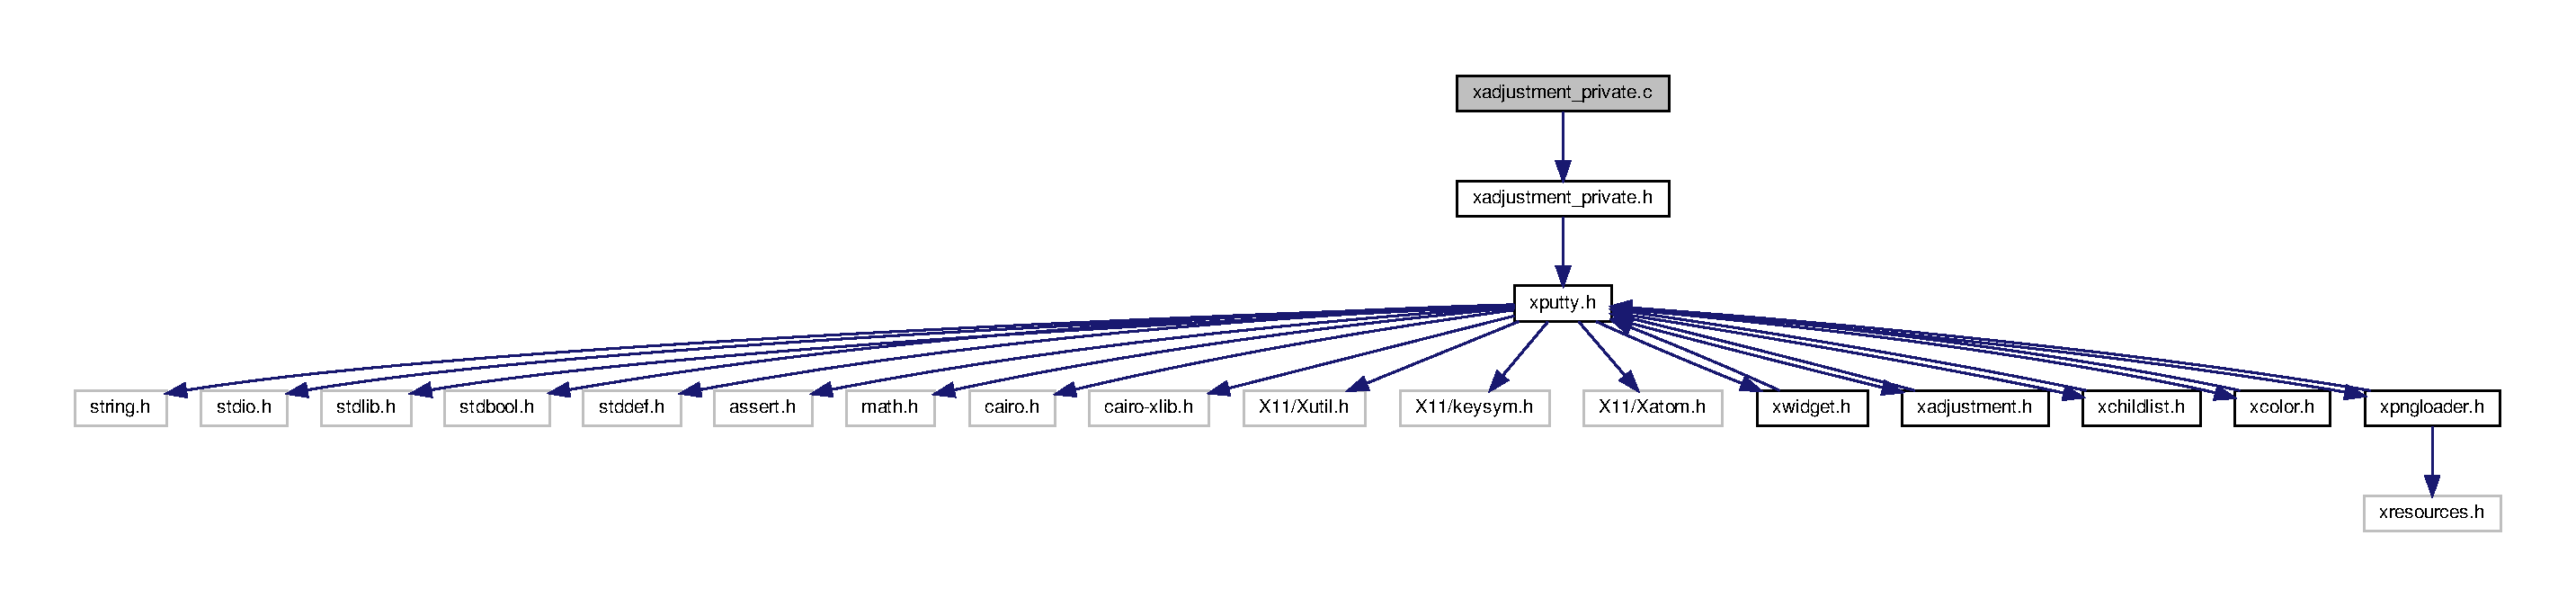
\includegraphics[width=350pt]{xadjustment__private_8c__incl}
\end{center}
\end{figure}
\subsection*{Functions}
\begin{DoxyCompactItemize}
\item 
void \hyperlink{xadjustment__private_8c_adbc6f7df16e0754fafab3a53ade544b2}{\+\_\+check\+\_\+value\+\_\+changed} (\hyperlink{structAdjustment__t}{Adjustment\+\_\+t} $\ast$adj, float $\ast$value)
\begin{DoxyCompactList}\small\item\em \+\_\+check\+\_\+value\+\_\+changed -\/ check if value has changed and send adj\+\_\+callback if so \end{DoxyCompactList}\end{DoxyCompactItemize}


\subsection{Function Documentation}
\mbox{\Hypertarget{xadjustment__private_8c_adbc6f7df16e0754fafab3a53ade544b2}\label{xadjustment__private_8c_adbc6f7df16e0754fafab3a53ade544b2}} 
\index{xadjustment\+\_\+private.\+c@{xadjustment\+\_\+private.\+c}!\+\_\+check\+\_\+value\+\_\+changed@{\+\_\+check\+\_\+value\+\_\+changed}}
\index{\+\_\+check\+\_\+value\+\_\+changed@{\+\_\+check\+\_\+value\+\_\+changed}!xadjustment\+\_\+private.\+c@{xadjustment\+\_\+private.\+c}}
\subsubsection{\texorpdfstring{\+\_\+check\+\_\+value\+\_\+changed()}{\_check\_value\_changed()}}
{\footnotesize\ttfamily void \+\_\+check\+\_\+value\+\_\+changed (\begin{DoxyParamCaption}\item[{\hyperlink{structAdjustment__t}{Adjustment\+\_\+t} $\ast$}]{adj,  }\item[{float $\ast$}]{value }\end{DoxyParamCaption})}



\+\_\+check\+\_\+value\+\_\+changed -\/ check if value has changed and send adj\+\_\+callback if so 


\begin{DoxyParams}{Parameters}
{\em $\ast$adj} & -\/ pointer to the Adjustment \\
\hline
{\em v} & -\/ value to check \\
\hline
\end{DoxyParams}
\begin{DoxyReturn}{Returns}
void 
\end{DoxyReturn}

\hypertarget{xadjustment__private_8h}{}\section{xadjustment\+\_\+private.\+h File Reference}
\label{xadjustment__private_8h}\index{xadjustment\+\_\+private.\+h@{xadjustment\+\_\+private.\+h}}
{\ttfamily \#include \char`\"{}xputty.\+h\char`\"{}}\newline
Include dependency graph for xadjustment\+\_\+private.\+h\+:
\nopagebreak
\begin{figure}[H]
\begin{center}
\leavevmode
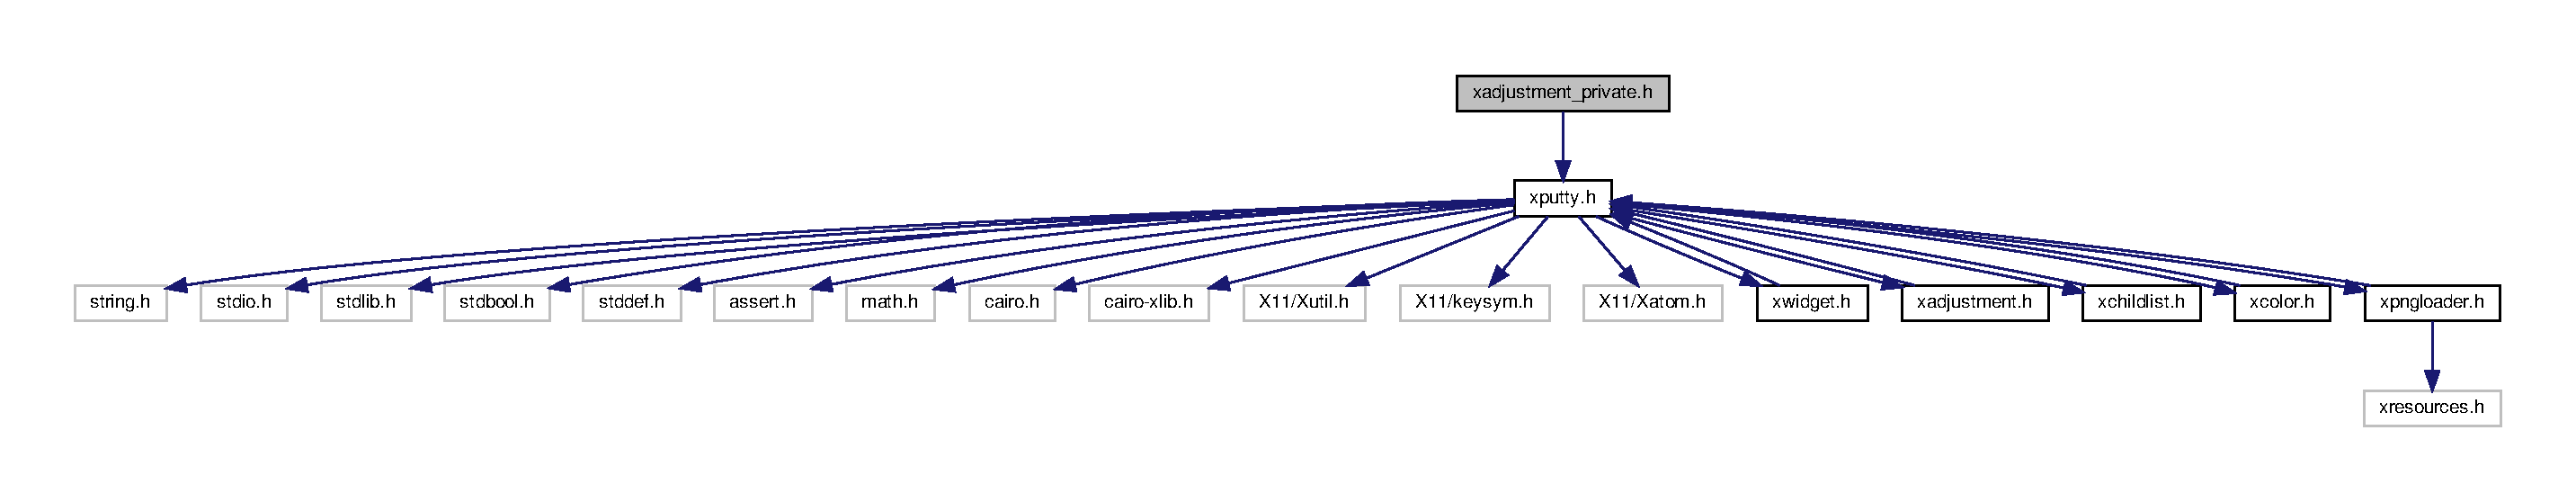
\includegraphics[width=350pt]{xadjustment__private_8h__incl}
\end{center}
\end{figure}
This graph shows which files directly or indirectly include this file\+:
\nopagebreak
\begin{figure}[H]
\begin{center}
\leavevmode
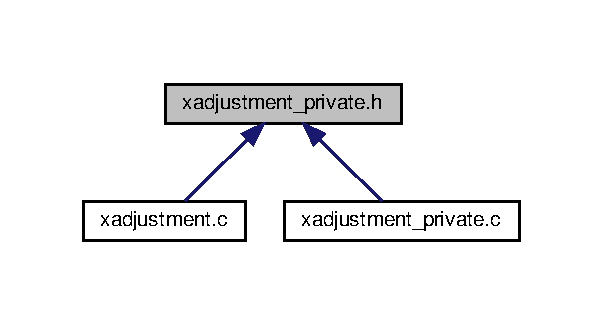
\includegraphics[width=290pt]{xadjustment__private_8h__dep__incl}
\end{center}
\end{figure}
\subsection*{Macros}
\begin{DoxyCompactItemize}
\item 
\#define \hyperlink{xadjustment__private_8h_a4a9187efbfbe9743bd49d9aa67928d0f}{X\+A\+D\+J\+U\+S\+T\+M\+E\+N\+T\+\_\+\+P\+R\+I\+V\+A\+T\+E\+\_\+\+H\+\_\+}
\end{DoxyCompactItemize}
\subsection*{Functions}
\begin{DoxyCompactItemize}
\item 
void \hyperlink{xadjustment__private_8h_adbc6f7df16e0754fafab3a53ade544b2}{\+\_\+check\+\_\+value\+\_\+changed} (\hyperlink{structAdjustment__t}{Adjustment\+\_\+t} $\ast$adj, float $\ast$value)
\begin{DoxyCompactList}\small\item\em \+\_\+check\+\_\+value\+\_\+changed -\/ check if value has changed and send adj\+\_\+callback if so \end{DoxyCompactList}\end{DoxyCompactItemize}


\subsection{Macro Definition Documentation}
\mbox{\Hypertarget{xadjustment__private_8h_a4a9187efbfbe9743bd49d9aa67928d0f}\label{xadjustment__private_8h_a4a9187efbfbe9743bd49d9aa67928d0f}} 
\index{xadjustment\+\_\+private.\+h@{xadjustment\+\_\+private.\+h}!X\+A\+D\+J\+U\+S\+T\+M\+E\+N\+T\+\_\+\+P\+R\+I\+V\+A\+T\+E\+\_\+\+H\+\_\+@{X\+A\+D\+J\+U\+S\+T\+M\+E\+N\+T\+\_\+\+P\+R\+I\+V\+A\+T\+E\+\_\+\+H\+\_\+}}
\index{X\+A\+D\+J\+U\+S\+T\+M\+E\+N\+T\+\_\+\+P\+R\+I\+V\+A\+T\+E\+\_\+\+H\+\_\+@{X\+A\+D\+J\+U\+S\+T\+M\+E\+N\+T\+\_\+\+P\+R\+I\+V\+A\+T\+E\+\_\+\+H\+\_\+}!xadjustment\+\_\+private.\+h@{xadjustment\+\_\+private.\+h}}
\subsubsection{\texorpdfstring{X\+A\+D\+J\+U\+S\+T\+M\+E\+N\+T\+\_\+\+P\+R\+I\+V\+A\+T\+E\+\_\+\+H\+\_\+}{XADJUSTMENT\_PRIVATE\_H\_}}
{\footnotesize\ttfamily \#define X\+A\+D\+J\+U\+S\+T\+M\+E\+N\+T\+\_\+\+P\+R\+I\+V\+A\+T\+E\+\_\+\+H\+\_\+}

here are the private functions from xadjustment 

\subsection{Function Documentation}
\mbox{\Hypertarget{xadjustment__private_8h_adbc6f7df16e0754fafab3a53ade544b2}\label{xadjustment__private_8h_adbc6f7df16e0754fafab3a53ade544b2}} 
\index{xadjustment\+\_\+private.\+h@{xadjustment\+\_\+private.\+h}!\+\_\+check\+\_\+value\+\_\+changed@{\+\_\+check\+\_\+value\+\_\+changed}}
\index{\+\_\+check\+\_\+value\+\_\+changed@{\+\_\+check\+\_\+value\+\_\+changed}!xadjustment\+\_\+private.\+h@{xadjustment\+\_\+private.\+h}}
\subsubsection{\texorpdfstring{\+\_\+check\+\_\+value\+\_\+changed()}{\_check\_value\_changed()}}
{\footnotesize\ttfamily void \+\_\+check\+\_\+value\+\_\+changed (\begin{DoxyParamCaption}\item[{\hyperlink{structAdjustment__t}{Adjustment\+\_\+t} $\ast$}]{adj,  }\item[{float $\ast$}]{value }\end{DoxyParamCaption})}



\+\_\+check\+\_\+value\+\_\+changed -\/ check if value has changed and send adj\+\_\+callback if so 


\begin{DoxyParams}{Parameters}
{\em $\ast$adj} & -\/ pointer to the Adjustment \\
\hline
{\em v} & -\/ value to check \\
\hline
\end{DoxyParams}
\begin{DoxyReturn}{Returns}
void 
\end{DoxyReturn}

\hypertarget{xbutton_8c}{}\section{xbutton.\+c File Reference}
\label{xbutton_8c}\index{xbutton.\+c@{xbutton.\+c}}
{\ttfamily \#include \char`\"{}xbutton.\+h\char`\"{}}\newline
{\ttfamily \#include \char`\"{}xbutton\+\_\+private.\+h\char`\"{}}\newline
Include dependency graph for xbutton.\+c\+:
\nopagebreak
\begin{figure}[H]
\begin{center}
\leavevmode
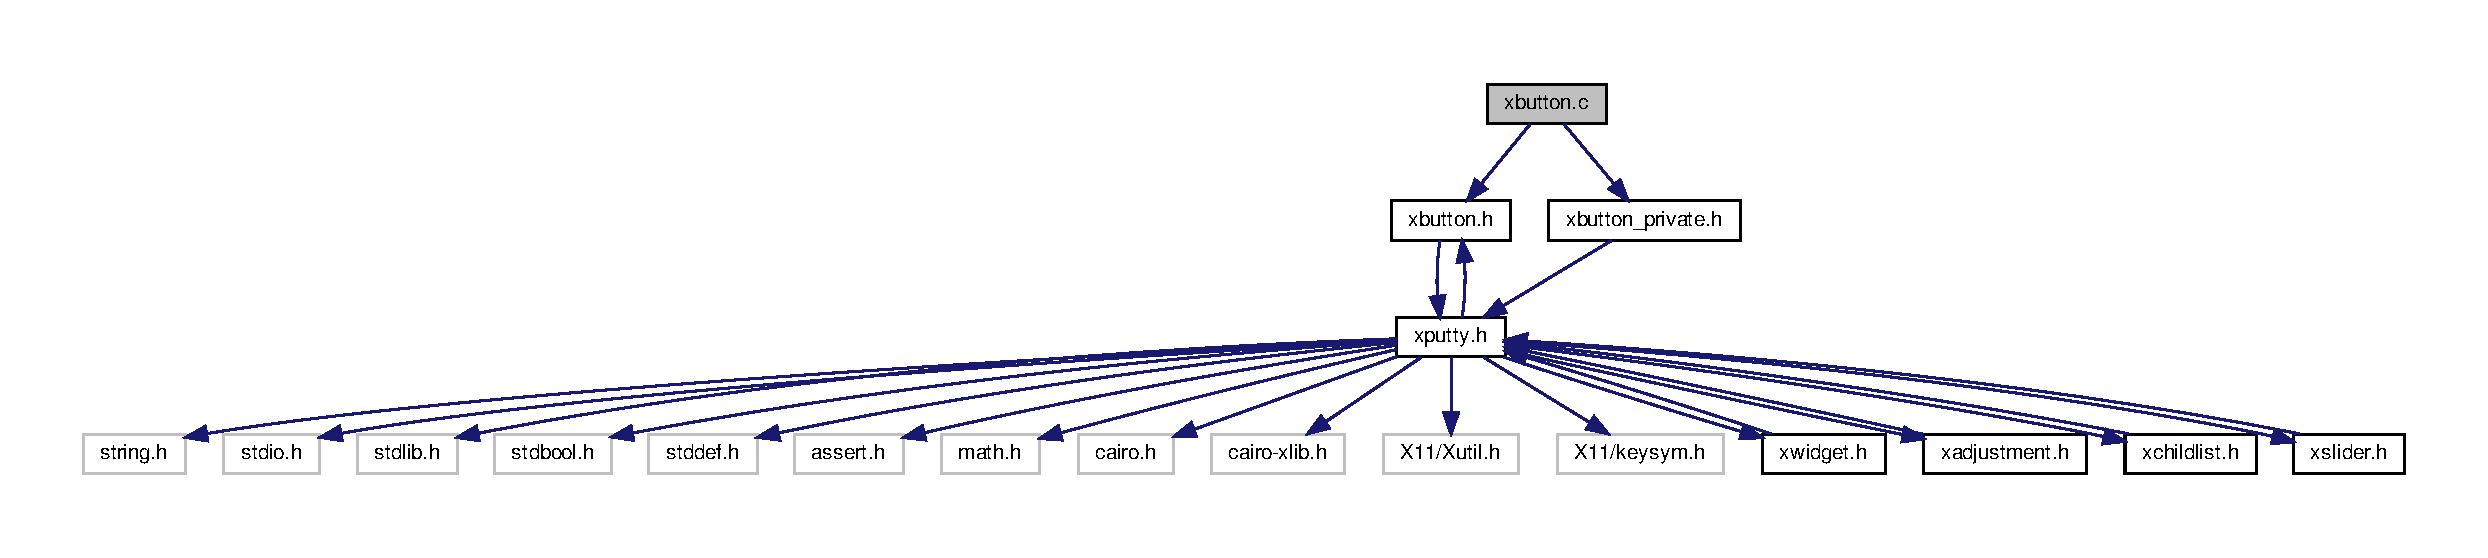
\includegraphics[width=350pt]{xbutton_8c__incl}
\end{center}
\end{figure}
\subsection*{Functions}
\begin{DoxyCompactItemize}
\item 
\hyperlink{structWidget__t}{Widget\+\_\+t} $\ast$ \hyperlink{xbutton_8c_a4dbd91e99d5ee97678aee121f8e12587}{add\+\_\+button} (\hyperlink{structWidget__t}{Widget\+\_\+t} $\ast$parent, const char $\ast$label, int x, int y, int width, int height)
\begin{DoxyCompactList}\small\item\em add\+\_\+button -\/ add a button to a \hyperlink{structWidget__t}{Widget\+\_\+t} connect to func.\+value\+\_\+changed\+\_\+callback to implement your actions \end{DoxyCompactList}\item 
\hyperlink{structWidget__t}{Widget\+\_\+t} $\ast$ \hyperlink{xbutton_8c_a528331e8ac24f1ca7bb0101dad28f962}{add\+\_\+toggle\+\_\+button} (\hyperlink{structWidget__t}{Widget\+\_\+t} $\ast$parent, const char $\ast$label, int x, int y, int width, int height)
\begin{DoxyCompactList}\small\item\em add\+\_\+toggle\+\_\+button -\/ add a button to a \hyperlink{structWidget__t}{Widget\+\_\+t} connect to func.\+value\+\_\+changed\+\_\+callback to implement your actions \end{DoxyCompactList}\end{DoxyCompactItemize}


\subsection{Function Documentation}
\mbox{\Hypertarget{xbutton_8c_a4dbd91e99d5ee97678aee121f8e12587}\label{xbutton_8c_a4dbd91e99d5ee97678aee121f8e12587}} 
\index{xbutton.\+c@{xbutton.\+c}!add\+\_\+button@{add\+\_\+button}}
\index{add\+\_\+button@{add\+\_\+button}!xbutton.\+c@{xbutton.\+c}}
\subsubsection{\texorpdfstring{add\+\_\+button()}{add\_button()}}
{\footnotesize\ttfamily \hyperlink{structWidget__t}{Widget\+\_\+t}$\ast$ add\+\_\+button (\begin{DoxyParamCaption}\item[{\hyperlink{structWidget__t}{Widget\+\_\+t} $\ast$}]{parent,  }\item[{const char $\ast$}]{label,  }\item[{int}]{x,  }\item[{int}]{y,  }\item[{int}]{width,  }\item[{int}]{height }\end{DoxyParamCaption})}



add\+\_\+button -\/ add a button to a \hyperlink{structWidget__t}{Widget\+\_\+t} connect to func.\+value\+\_\+changed\+\_\+callback to implement your actions 


\begin{DoxyParams}{Parameters}
{\em $\ast$parent} & -\/ pointer to the \hyperlink{structWidget__t}{Widget\+\_\+t} request the button \\
\hline
{\em $\ast$label} & -\/ Label to show on the button \\
\hline
{\em x,y,width,height} & -\/ the position/geometry to create the button \\
\hline
\end{DoxyParams}
\begin{DoxyReturn}{Returns}
Widget\+\_\+t$\ast$ -\/ pointer to the \hyperlink{structWidget__t}{Widget\+\_\+t} button struct 
\end{DoxyReturn}
\mbox{\Hypertarget{xbutton_8c_a528331e8ac24f1ca7bb0101dad28f962}\label{xbutton_8c_a528331e8ac24f1ca7bb0101dad28f962}} 
\index{xbutton.\+c@{xbutton.\+c}!add\+\_\+toggle\+\_\+button@{add\+\_\+toggle\+\_\+button}}
\index{add\+\_\+toggle\+\_\+button@{add\+\_\+toggle\+\_\+button}!xbutton.\+c@{xbutton.\+c}}
\subsubsection{\texorpdfstring{add\+\_\+toggle\+\_\+button()}{add\_toggle\_button()}}
{\footnotesize\ttfamily \hyperlink{structWidget__t}{Widget\+\_\+t}$\ast$ add\+\_\+toggle\+\_\+button (\begin{DoxyParamCaption}\item[{\hyperlink{structWidget__t}{Widget\+\_\+t} $\ast$}]{parent,  }\item[{const char $\ast$}]{label,  }\item[{int}]{x,  }\item[{int}]{y,  }\item[{int}]{width,  }\item[{int}]{height }\end{DoxyParamCaption})}



add\+\_\+toggle\+\_\+button -\/ add a button to a \hyperlink{structWidget__t}{Widget\+\_\+t} connect to func.\+value\+\_\+changed\+\_\+callback to implement your actions 


\begin{DoxyParams}{Parameters}
{\em $\ast$parent} & -\/ pointer to the \hyperlink{structWidget__t}{Widget\+\_\+t} request the button \\
\hline
{\em $\ast$label} & -\/ Label to show on the button \\
\hline
{\em x,y,width,height} & -\/ the position/geometry to create the button \\
\hline
\end{DoxyParams}
\begin{DoxyReturn}{Returns}
Widget\+\_\+t$\ast$ -\/ pointer to the \hyperlink{structWidget__t}{Widget\+\_\+t} button struct 
\end{DoxyReturn}

\hypertarget{xbutton_8h}{}\section{xbutton.\+h File Reference}
\label{xbutton_8h}\index{xbutton.\+h@{xbutton.\+h}}
{\ttfamily \#include \char`\"{}xputty.\+h\char`\"{}}\newline
Include dependency graph for xbutton.\+h\+:
\nopagebreak
\begin{figure}[H]
\begin{center}
\leavevmode
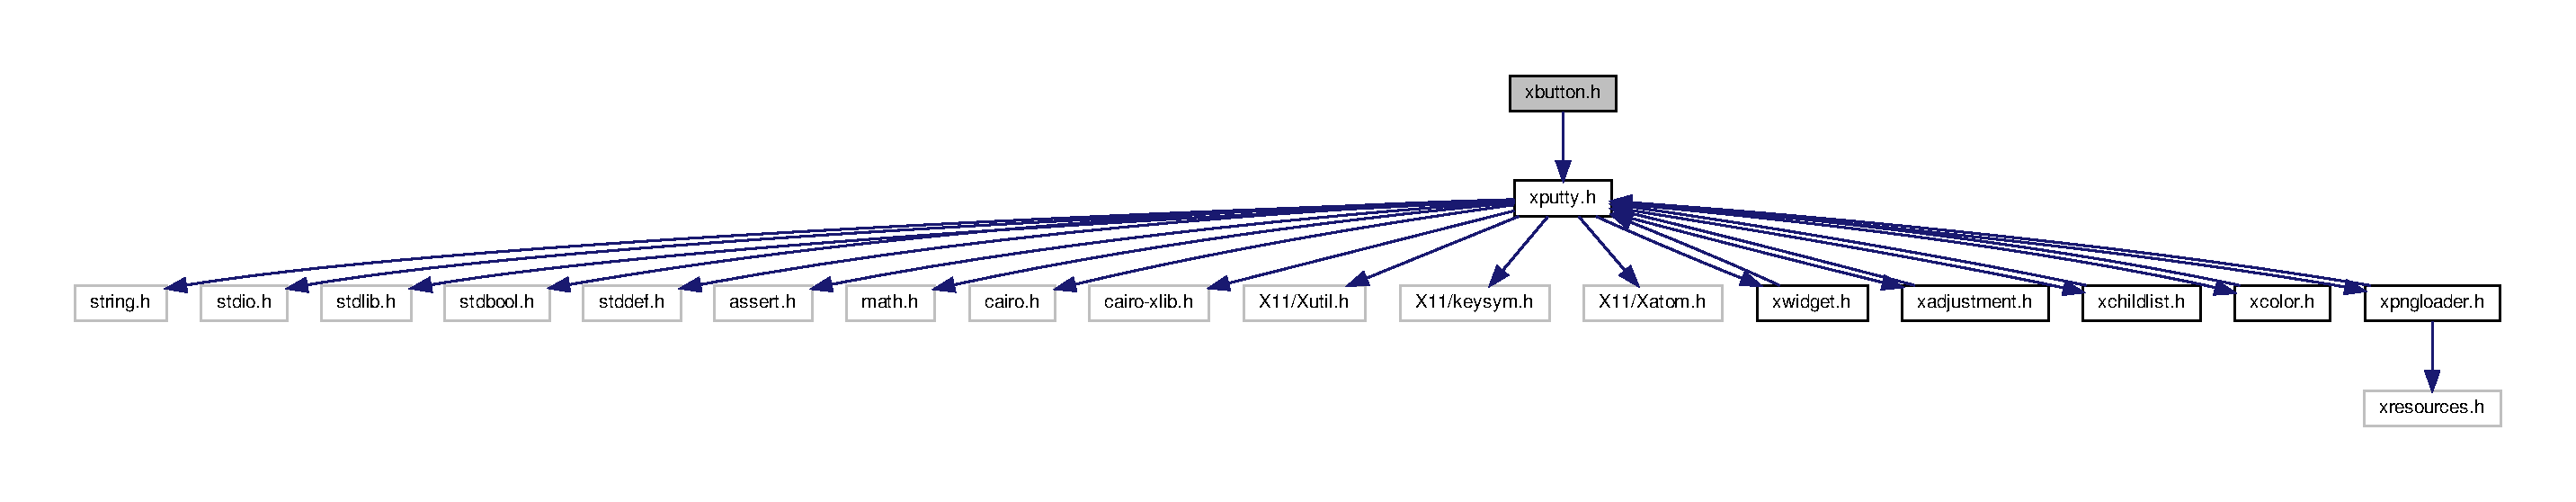
\includegraphics[width=350pt]{xbutton_8h__incl}
\end{center}
\end{figure}
This graph shows which files directly or indirectly include this file\+:
\nopagebreak
\begin{figure}[H]
\begin{center}
\leavevmode
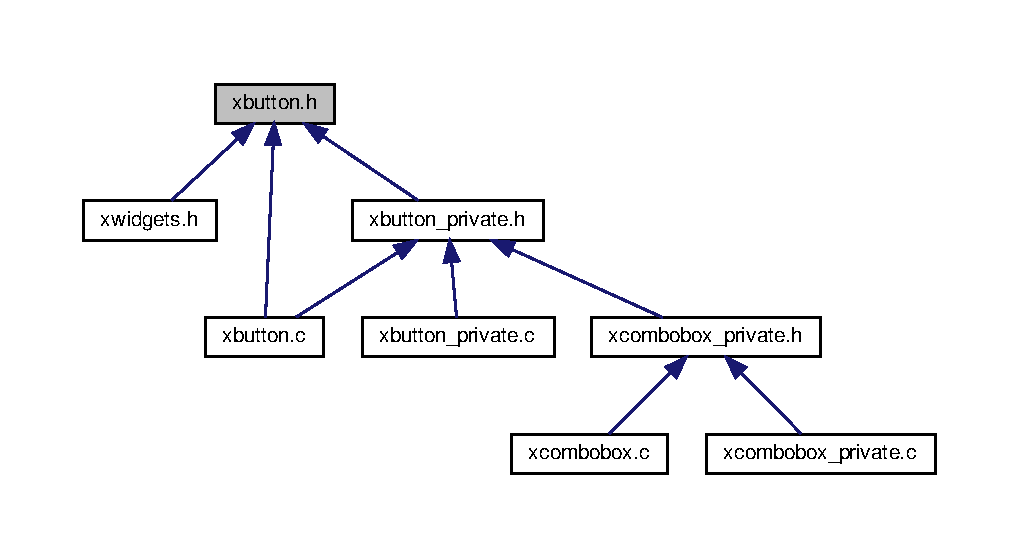
\includegraphics[width=350pt]{xbutton_8h__dep__incl}
\end{center}
\end{figure}
\subsection*{Macros}
\begin{DoxyCompactItemize}
\item 
\#define \hyperlink{xbutton_8h_a529495b7491220cdb4cf420183099430}{X\+B\+U\+T\+T\+O\+N\+\_\+\+H\+\_\+}
\end{DoxyCompactItemize}
\subsection*{Functions}
\begin{DoxyCompactItemize}
\item 
\hyperlink{structWidget__t}{Widget\+\_\+t} $\ast$ \hyperlink{xbutton_8h_a4dbd91e99d5ee97678aee121f8e12587}{add\+\_\+button} (\hyperlink{structWidget__t}{Widget\+\_\+t} $\ast$parent, const char $\ast$label, int x, int y, int width, int height)
\begin{DoxyCompactList}\small\item\em add\+\_\+button -\/ add a button to a \hyperlink{structWidget__t}{Widget\+\_\+t} connect to func.\+value\+\_\+changed\+\_\+callback to implement your actions \end{DoxyCompactList}\item 
\hyperlink{structWidget__t}{Widget\+\_\+t} $\ast$ \hyperlink{xbutton_8h_a528331e8ac24f1ca7bb0101dad28f962}{add\+\_\+toggle\+\_\+button} (\hyperlink{structWidget__t}{Widget\+\_\+t} $\ast$parent, const char $\ast$label, int x, int y, int width, int height)
\begin{DoxyCompactList}\small\item\em add\+\_\+toggle\+\_\+button -\/ add a button to a \hyperlink{structWidget__t}{Widget\+\_\+t} connect to func.\+value\+\_\+changed\+\_\+callback to implement your actions \end{DoxyCompactList}\end{DoxyCompactItemize}


\subsection{Macro Definition Documentation}
\mbox{\Hypertarget{xbutton_8h_a529495b7491220cdb4cf420183099430}\label{xbutton_8h_a529495b7491220cdb4cf420183099430}} 
\index{xbutton.\+h@{xbutton.\+h}!X\+B\+U\+T\+T\+O\+N\+\_\+\+H\+\_\+@{X\+B\+U\+T\+T\+O\+N\+\_\+\+H\+\_\+}}
\index{X\+B\+U\+T\+T\+O\+N\+\_\+\+H\+\_\+@{X\+B\+U\+T\+T\+O\+N\+\_\+\+H\+\_\+}!xbutton.\+h@{xbutton.\+h}}
\subsubsection{\texorpdfstring{X\+B\+U\+T\+T\+O\+N\+\_\+\+H\+\_\+}{XBUTTON\_H\_}}
{\footnotesize\ttfamily \#define X\+B\+U\+T\+T\+O\+N\+\_\+\+H\+\_\+}



\subsection{Function Documentation}
\mbox{\Hypertarget{xbutton_8h_a4dbd91e99d5ee97678aee121f8e12587}\label{xbutton_8h_a4dbd91e99d5ee97678aee121f8e12587}} 
\index{xbutton.\+h@{xbutton.\+h}!add\+\_\+button@{add\+\_\+button}}
\index{add\+\_\+button@{add\+\_\+button}!xbutton.\+h@{xbutton.\+h}}
\subsubsection{\texorpdfstring{add\+\_\+button()}{add\_button()}}
{\footnotesize\ttfamily \hyperlink{structWidget__t}{Widget\+\_\+t}$\ast$ add\+\_\+button (\begin{DoxyParamCaption}\item[{\hyperlink{structWidget__t}{Widget\+\_\+t} $\ast$}]{parent,  }\item[{const char $\ast$}]{label,  }\item[{int}]{x,  }\item[{int}]{y,  }\item[{int}]{width,  }\item[{int}]{height }\end{DoxyParamCaption})}



add\+\_\+button -\/ add a button to a \hyperlink{structWidget__t}{Widget\+\_\+t} connect to func.\+value\+\_\+changed\+\_\+callback to implement your actions 


\begin{DoxyParams}{Parameters}
{\em $\ast$parent} & -\/ pointer to the \hyperlink{structWidget__t}{Widget\+\_\+t} request the button \\
\hline
{\em $\ast$label} & -\/ Label to show on the button \\
\hline
{\em x,y,width,height} & -\/ the position/geometry to create the button \\
\hline
\end{DoxyParams}
\begin{DoxyReturn}{Returns}
Widget\+\_\+t$\ast$ -\/ pointer to the \hyperlink{structWidget__t}{Widget\+\_\+t} button struct 
\end{DoxyReturn}
\mbox{\Hypertarget{xbutton_8h_a528331e8ac24f1ca7bb0101dad28f962}\label{xbutton_8h_a528331e8ac24f1ca7bb0101dad28f962}} 
\index{xbutton.\+h@{xbutton.\+h}!add\+\_\+toggle\+\_\+button@{add\+\_\+toggle\+\_\+button}}
\index{add\+\_\+toggle\+\_\+button@{add\+\_\+toggle\+\_\+button}!xbutton.\+h@{xbutton.\+h}}
\subsubsection{\texorpdfstring{add\+\_\+toggle\+\_\+button()}{add\_toggle\_button()}}
{\footnotesize\ttfamily \hyperlink{structWidget__t}{Widget\+\_\+t}$\ast$ add\+\_\+toggle\+\_\+button (\begin{DoxyParamCaption}\item[{\hyperlink{structWidget__t}{Widget\+\_\+t} $\ast$}]{parent,  }\item[{const char $\ast$}]{label,  }\item[{int}]{x,  }\item[{int}]{y,  }\item[{int}]{width,  }\item[{int}]{height }\end{DoxyParamCaption})}



add\+\_\+toggle\+\_\+button -\/ add a button to a \hyperlink{structWidget__t}{Widget\+\_\+t} connect to func.\+value\+\_\+changed\+\_\+callback to implement your actions 


\begin{DoxyParams}{Parameters}
{\em $\ast$parent} & -\/ pointer to the \hyperlink{structWidget__t}{Widget\+\_\+t} request the button \\
\hline
{\em $\ast$label} & -\/ Label to show on the button \\
\hline
{\em x,y,width,height} & -\/ the position/geometry to create the button \\
\hline
\end{DoxyParams}
\begin{DoxyReturn}{Returns}
Widget\+\_\+t$\ast$ -\/ pointer to the \hyperlink{structWidget__t}{Widget\+\_\+t} button struct 
\end{DoxyReturn}

\hypertarget{xbutton__private_8c}{}\section{xbutton\+\_\+private.\+c File Reference}
\label{xbutton__private_8c}\index{xbutton\+\_\+private.\+c@{xbutton\+\_\+private.\+c}}
{\ttfamily \#include \char`\"{}xbutton\+\_\+private.\+h\char`\"{}}\newline
Include dependency graph for xbutton\+\_\+private.\+c\+:
\nopagebreak
\begin{figure}[H]
\begin{center}
\leavevmode
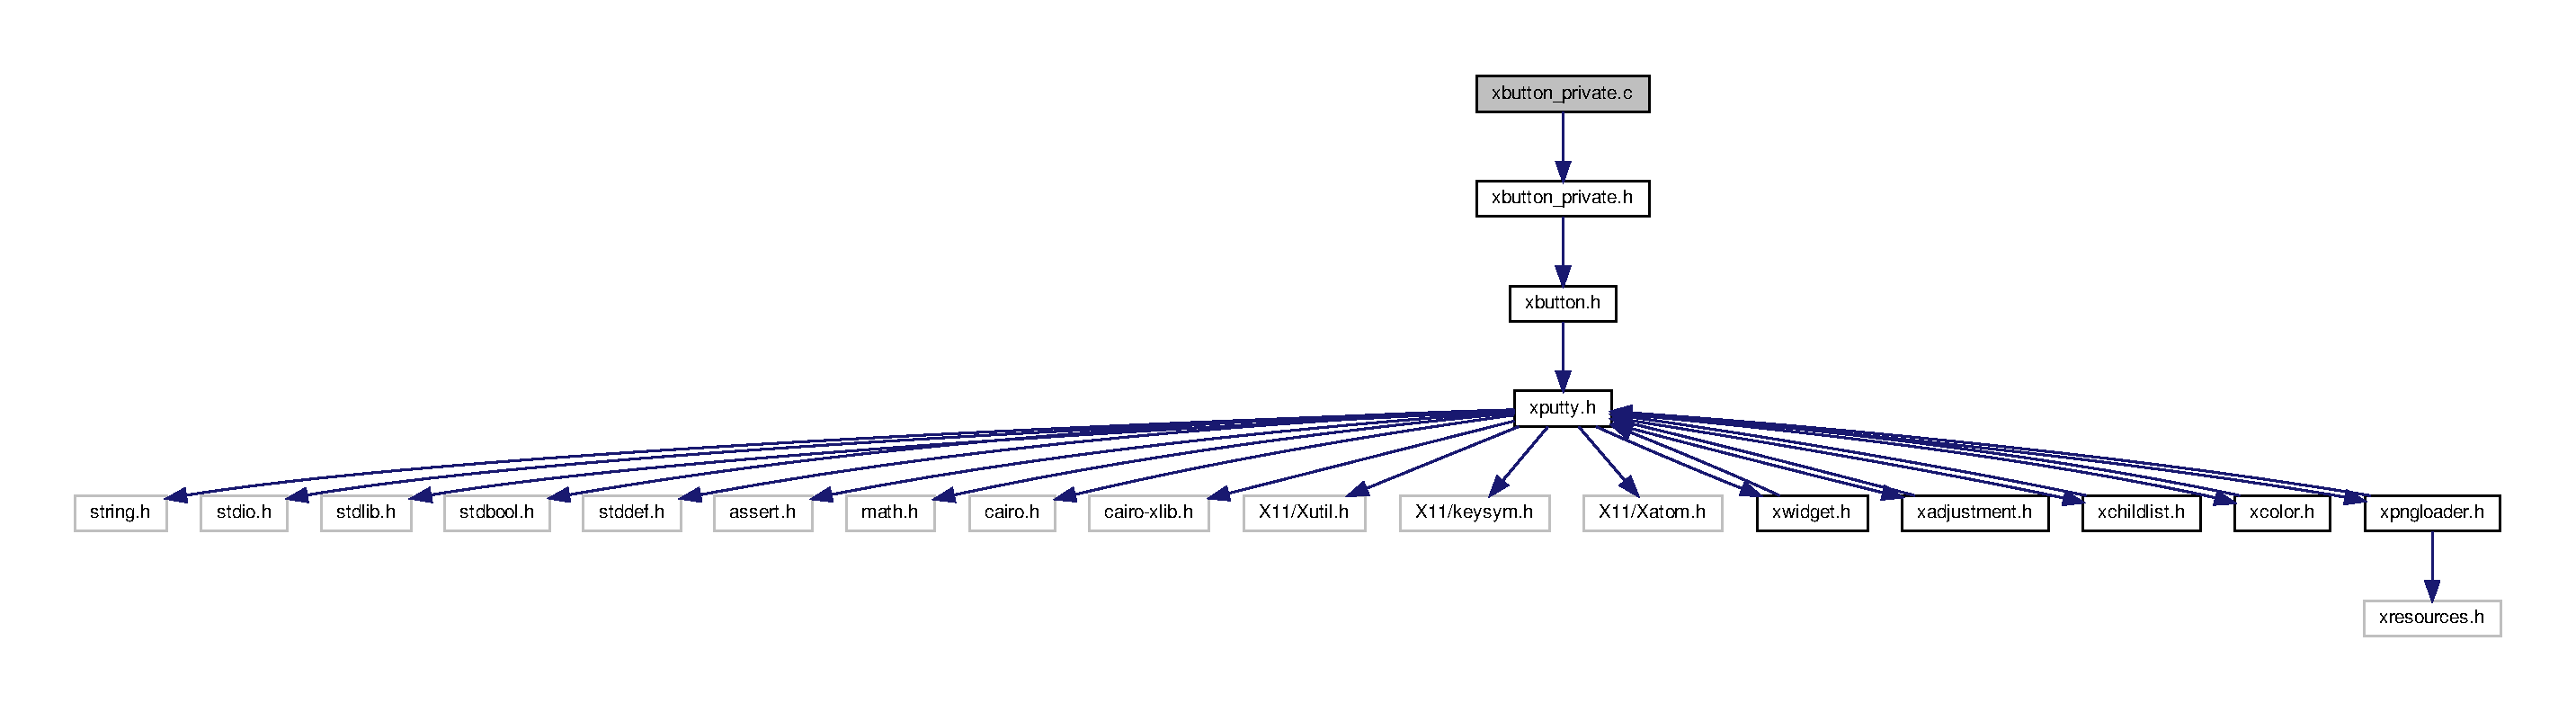
\includegraphics[width=350pt]{xbutton__private_8c__incl}
\end{center}
\end{figure}
\subsection*{Functions}
\begin{DoxyCompactItemize}
\item 
void \hyperlink{xbutton__private_8c_a84ad14c8ee4ef96c7d92acc972883c8b}{\+\_\+set\+\_\+button\+\_\+colormap} (\hyperlink{structWidget__t}{Widget\+\_\+t} $\ast$wid)
\begin{DoxyCompactList}\small\item\em \+\_\+set\+\_\+button\+\_\+colormap -\/ set color map to use for button states \end{DoxyCompactList}\item 
void \hyperlink{xbutton__private_8c_ad4e31fc35cac78b036b693d09edfad35}{\+\_\+rounded\+\_\+rectangle} (cairo\+\_\+t $\ast$cr, float x, float y, float width, float height)
\begin{DoxyCompactList}\small\item\em \+\_\+rounded\+\_\+rectangle -\/ internal draw a rounded button \end{DoxyCompactList}\item 
void \hyperlink{xbutton__private_8c_ac0888b19e35a96f7820b87f3e2316ec2}{\+\_\+pattern\+\_\+out} (\hyperlink{structWidget__t}{Widget\+\_\+t} $\ast$w, \hyperlink{xwidget_8h_a8a9a00ba3976b54d9c5cacffe16d14ef}{Widget\+\_\+state} st, int height)
\begin{DoxyCompactList}\small\item\em \+\_\+pattern\+\_\+in -\/ a little pattern to make press state more visible \end{DoxyCompactList}\item 
void \hyperlink{xbutton__private_8c_a646ed35fa047cfcc7a93d1790c672fc1}{\+\_\+pattern\+\_\+in} (\hyperlink{structWidget__t}{Widget\+\_\+t} $\ast$w, \hyperlink{xwidget_8h_a8a9a00ba3976b54d9c5cacffe16d14ef}{Widget\+\_\+state} st, int height)
\begin{DoxyCompactList}\small\item\em \+\_\+pattern\+\_\+in -\/ a little pattern to make press state more visible \end{DoxyCompactList}\item 
void \hyperlink{xbutton__private_8c_a555079b56b3d52f2a74c20f6ebd05e29}{\+\_\+draw\+\_\+button} (void $\ast$w\+\_\+, void $\ast$user\+\_\+data)
\begin{DoxyCompactList}\small\item\em \+\_\+draw\+\_\+button -\/ internal draw the button to the buffer \end{DoxyCompactList}\item 
void \hyperlink{xbutton__private_8c_a28a4fe06426208c720b93c1fa51aff49}{\+\_\+button\+\_\+pressed} (void $\ast$w\+\_\+, void $\ast$button, void $\ast$user\+\_\+data)
\begin{DoxyCompactList}\small\item\em \+\_\+button\+\_\+pressed -\/ redraw the button and send state via user\+\_\+callback \end{DoxyCompactList}\item 
void \hyperlink{xbutton__private_8c_a0168623590cbb3b5f19ae0878ea41a5f}{\+\_\+button\+\_\+released} (void $\ast$w\+\_\+, void $\ast$button\+\_\+, void $\ast$user\+\_\+data)
\begin{DoxyCompactList}\small\item\em \+\_\+button\+\_\+released -\/ redraw the button and send state via user\+\_\+callback \end{DoxyCompactList}\item 
void \hyperlink{xbutton__private_8c_a31d787399bcdba7f2589a9499d45695f}{\+\_\+toggle\+\_\+button\+\_\+pressed} (void $\ast$w\+\_\+, void $\ast$button, void $\ast$user\+\_\+data)
\begin{DoxyCompactList}\small\item\em \+\_\+toggle\+\_\+button\+\_\+pressed -\/ redraw the button and send state via user\+\_\+callback \end{DoxyCompactList}\item 
void \hyperlink{xbutton__private_8c_a0aed08450617940038e61344f5d67743}{\+\_\+toggle\+\_\+button\+\_\+released} (void $\ast$w\+\_\+, void $\ast$button\+\_\+, void $\ast$user\+\_\+data)
\begin{DoxyCompactList}\small\item\em \+\_\+toggle\+\_\+button\+\_\+released -\/ redraw the button and send state via user\+\_\+callback \end{DoxyCompactList}\end{DoxyCompactItemize}


\subsection{Function Documentation}
\mbox{\Hypertarget{xbutton__private_8c_a28a4fe06426208c720b93c1fa51aff49}\label{xbutton__private_8c_a28a4fe06426208c720b93c1fa51aff49}} 
\index{xbutton\+\_\+private.\+c@{xbutton\+\_\+private.\+c}!\+\_\+button\+\_\+pressed@{\+\_\+button\+\_\+pressed}}
\index{\+\_\+button\+\_\+pressed@{\+\_\+button\+\_\+pressed}!xbutton\+\_\+private.\+c@{xbutton\+\_\+private.\+c}}
\subsubsection{\texorpdfstring{\+\_\+button\+\_\+pressed()}{\_button\_pressed()}}
{\footnotesize\ttfamily void \+\_\+button\+\_\+pressed (\begin{DoxyParamCaption}\item[{void $\ast$}]{w\+\_\+,  }\item[{void $\ast$}]{button,  }\item[{void $\ast$}]{user\+\_\+data }\end{DoxyParamCaption})}



\+\_\+button\+\_\+pressed -\/ redraw the button and send state via user\+\_\+callback 


\begin{DoxyParams}{Parameters}
{\em $\ast$w\+\_\+} & -\/ void pointer to the \hyperlink{structWidget__t}{Widget\+\_\+t} button \\
\hline
{\em $\ast$button} & -\/ void pointer to X\+Event.\+xbutton struct \\
\hline
{\em $\ast$user\+\_\+data} & -\/ void pointer to attached user\+\_\+data \\
\hline
\end{DoxyParams}
\begin{DoxyReturn}{Returns}
void 
\end{DoxyReturn}
\mbox{\Hypertarget{xbutton__private_8c_a0168623590cbb3b5f19ae0878ea41a5f}\label{xbutton__private_8c_a0168623590cbb3b5f19ae0878ea41a5f}} 
\index{xbutton\+\_\+private.\+c@{xbutton\+\_\+private.\+c}!\+\_\+button\+\_\+released@{\+\_\+button\+\_\+released}}
\index{\+\_\+button\+\_\+released@{\+\_\+button\+\_\+released}!xbutton\+\_\+private.\+c@{xbutton\+\_\+private.\+c}}
\subsubsection{\texorpdfstring{\+\_\+button\+\_\+released()}{\_button\_released()}}
{\footnotesize\ttfamily void \+\_\+button\+\_\+released (\begin{DoxyParamCaption}\item[{void $\ast$}]{w\+\_\+,  }\item[{void $\ast$}]{button\+\_\+,  }\item[{void $\ast$}]{user\+\_\+data }\end{DoxyParamCaption})}



\+\_\+button\+\_\+released -\/ redraw the button and send state via user\+\_\+callback 


\begin{DoxyParams}{Parameters}
{\em $\ast$w\+\_\+} & -\/ void pointer to the \hyperlink{structWidget__t}{Widget\+\_\+t} button \\
\hline
{\em $\ast$button} & -\/ void pointer to X\+Event.\+xbutton struct \\
\hline
{\em $\ast$user\+\_\+data} & -\/ void pointer to attached user\+\_\+data \\
\hline
\end{DoxyParams}
\begin{DoxyReturn}{Returns}
void 
\end{DoxyReturn}
\mbox{\Hypertarget{xbutton__private_8c_a555079b56b3d52f2a74c20f6ebd05e29}\label{xbutton__private_8c_a555079b56b3d52f2a74c20f6ebd05e29}} 
\index{xbutton\+\_\+private.\+c@{xbutton\+\_\+private.\+c}!\+\_\+draw\+\_\+button@{\+\_\+draw\+\_\+button}}
\index{\+\_\+draw\+\_\+button@{\+\_\+draw\+\_\+button}!xbutton\+\_\+private.\+c@{xbutton\+\_\+private.\+c}}
\subsubsection{\texorpdfstring{\+\_\+draw\+\_\+button()}{\_draw\_button()}}
{\footnotesize\ttfamily void \+\_\+draw\+\_\+button (\begin{DoxyParamCaption}\item[{void $\ast$}]{w\+\_\+,  }\item[{void $\ast$}]{user\+\_\+data }\end{DoxyParamCaption})}



\+\_\+draw\+\_\+button -\/ internal draw the button to the buffer 


\begin{DoxyParams}{Parameters}
{\em $\ast$w\+\_\+} & -\/ void pointer to the \hyperlink{structWidget__t}{Widget\+\_\+t} button \\
\hline
{\em $\ast$user\+\_\+data} & -\/ void pointer to attached user\+\_\+data \\
\hline
\end{DoxyParams}
\begin{DoxyReturn}{Returns}
void 
\end{DoxyReturn}
\mbox{\Hypertarget{xbutton__private_8c_a646ed35fa047cfcc7a93d1790c672fc1}\label{xbutton__private_8c_a646ed35fa047cfcc7a93d1790c672fc1}} 
\index{xbutton\+\_\+private.\+c@{xbutton\+\_\+private.\+c}!\+\_\+pattern\+\_\+in@{\+\_\+pattern\+\_\+in}}
\index{\+\_\+pattern\+\_\+in@{\+\_\+pattern\+\_\+in}!xbutton\+\_\+private.\+c@{xbutton\+\_\+private.\+c}}
\subsubsection{\texorpdfstring{\+\_\+pattern\+\_\+in()}{\_pattern\_in()}}
{\footnotesize\ttfamily void \+\_\+pattern\+\_\+in (\begin{DoxyParamCaption}\item[{\hyperlink{structWidget__t}{Widget\+\_\+t} $\ast$}]{w,  }\item[{\hyperlink{xwidget_8h_a8a9a00ba3976b54d9c5cacffe16d14ef}{Widget\+\_\+state}}]{st,  }\item[{int}]{height }\end{DoxyParamCaption})}



\+\_\+pattern\+\_\+in -\/ a little pattern to make press state more visible 


\begin{DoxyParams}{Parameters}
{\em $\ast$w\+\_\+} & -\/ void pointer to the \hyperlink{structWidget__t}{Widget\+\_\+t} button \\
\hline
{\em st} & -\/ the color state to use \\
\hline
{\em height} & -\/ the button height \\
\hline
\end{DoxyParams}
\begin{DoxyReturn}{Returns}
void 
\end{DoxyReturn}
\mbox{\Hypertarget{xbutton__private_8c_ac0888b19e35a96f7820b87f3e2316ec2}\label{xbutton__private_8c_ac0888b19e35a96f7820b87f3e2316ec2}} 
\index{xbutton\+\_\+private.\+c@{xbutton\+\_\+private.\+c}!\+\_\+pattern\+\_\+out@{\+\_\+pattern\+\_\+out}}
\index{\+\_\+pattern\+\_\+out@{\+\_\+pattern\+\_\+out}!xbutton\+\_\+private.\+c@{xbutton\+\_\+private.\+c}}
\subsubsection{\texorpdfstring{\+\_\+pattern\+\_\+out()}{\_pattern\_out()}}
{\footnotesize\ttfamily void \+\_\+pattern\+\_\+out (\begin{DoxyParamCaption}\item[{\hyperlink{structWidget__t}{Widget\+\_\+t} $\ast$}]{w,  }\item[{\hyperlink{xwidget_8h_a8a9a00ba3976b54d9c5cacffe16d14ef}{Widget\+\_\+state}}]{st,  }\item[{int}]{height }\end{DoxyParamCaption})}



\+\_\+pattern\+\_\+in -\/ a little pattern to make press state more visible 


\begin{DoxyParams}{Parameters}
{\em $\ast$w\+\_\+} & -\/ void pointer to the \hyperlink{structWidget__t}{Widget\+\_\+t} button \\
\hline
{\em st} & -\/ the color state to use \\
\hline
{\em height} & -\/ the button height \\
\hline
\end{DoxyParams}
\begin{DoxyReturn}{Returns}
void 
\end{DoxyReturn}
\mbox{\Hypertarget{xbutton__private_8c_ad4e31fc35cac78b036b693d09edfad35}\label{xbutton__private_8c_ad4e31fc35cac78b036b693d09edfad35}} 
\index{xbutton\+\_\+private.\+c@{xbutton\+\_\+private.\+c}!\+\_\+rounded\+\_\+rectangle@{\+\_\+rounded\+\_\+rectangle}}
\index{\+\_\+rounded\+\_\+rectangle@{\+\_\+rounded\+\_\+rectangle}!xbutton\+\_\+private.\+c@{xbutton\+\_\+private.\+c}}
\subsubsection{\texorpdfstring{\+\_\+rounded\+\_\+rectangle()}{\_rounded\_rectangle()}}
{\footnotesize\ttfamily void \+\_\+rounded\+\_\+rectangle (\begin{DoxyParamCaption}\item[{cairo\+\_\+t $\ast$}]{cr,  }\item[{float}]{x,  }\item[{float}]{y,  }\item[{float}]{width,  }\item[{float}]{height }\end{DoxyParamCaption})}



\+\_\+rounded\+\_\+rectangle -\/ internal draw a rounded button 


\begin{DoxyParams}{Parameters}
{\em x} & -\/ point on x axis \\
\hline
{\em y} & -\/ point on y axis \\
\hline
{\em width} & -\/ the button width \\
\hline
{\em height} & -\/ the button height \\
\hline
\end{DoxyParams}
\begin{DoxyReturn}{Returns}
void 
\end{DoxyReturn}
\mbox{\Hypertarget{xbutton__private_8c_a84ad14c8ee4ef96c7d92acc972883c8b}\label{xbutton__private_8c_a84ad14c8ee4ef96c7d92acc972883c8b}} 
\index{xbutton\+\_\+private.\+c@{xbutton\+\_\+private.\+c}!\+\_\+set\+\_\+button\+\_\+colormap@{\+\_\+set\+\_\+button\+\_\+colormap}}
\index{\+\_\+set\+\_\+button\+\_\+colormap@{\+\_\+set\+\_\+button\+\_\+colormap}!xbutton\+\_\+private.\+c@{xbutton\+\_\+private.\+c}}
\subsubsection{\texorpdfstring{\+\_\+set\+\_\+button\+\_\+colormap()}{\_set\_button\_colormap()}}
{\footnotesize\ttfamily void \+\_\+set\+\_\+button\+\_\+colormap (\begin{DoxyParamCaption}\item[{\hyperlink{structWidget__t}{Widget\+\_\+t} $\ast$}]{wid }\end{DoxyParamCaption})}



\+\_\+set\+\_\+button\+\_\+colormap -\/ set color map to use for button states 


\begin{DoxyParams}{Parameters}
{\em $\ast$wid} & -\/ pointer to \hyperlink{structWidget__t}{Widget\+\_\+t} \\
\hline
\end{DoxyParams}
\begin{DoxyReturn}{Returns}
void 
\end{DoxyReturn}
\mbox{\Hypertarget{xbutton__private_8c_a31d787399bcdba7f2589a9499d45695f}\label{xbutton__private_8c_a31d787399bcdba7f2589a9499d45695f}} 
\index{xbutton\+\_\+private.\+c@{xbutton\+\_\+private.\+c}!\+\_\+toggle\+\_\+button\+\_\+pressed@{\+\_\+toggle\+\_\+button\+\_\+pressed}}
\index{\+\_\+toggle\+\_\+button\+\_\+pressed@{\+\_\+toggle\+\_\+button\+\_\+pressed}!xbutton\+\_\+private.\+c@{xbutton\+\_\+private.\+c}}
\subsubsection{\texorpdfstring{\+\_\+toggle\+\_\+button\+\_\+pressed()}{\_toggle\_button\_pressed()}}
{\footnotesize\ttfamily void \+\_\+toggle\+\_\+button\+\_\+pressed (\begin{DoxyParamCaption}\item[{void $\ast$}]{w\+\_\+,  }\item[{void $\ast$}]{button,  }\item[{void $\ast$}]{user\+\_\+data }\end{DoxyParamCaption})}



\+\_\+toggle\+\_\+button\+\_\+pressed -\/ redraw the button and send state via user\+\_\+callback 


\begin{DoxyParams}{Parameters}
{\em $\ast$w\+\_\+} & -\/ void pointer to the \hyperlink{structWidget__t}{Widget\+\_\+t} button \\
\hline
{\em $\ast$button} & -\/ void pointer to X\+Event.\+xbutton struct \\
\hline
{\em $\ast$user\+\_\+data} & -\/ void pointer to attached user\+\_\+data \\
\hline
\end{DoxyParams}
\begin{DoxyReturn}{Returns}
void 
\end{DoxyReturn}
\mbox{\Hypertarget{xbutton__private_8c_a0aed08450617940038e61344f5d67743}\label{xbutton__private_8c_a0aed08450617940038e61344f5d67743}} 
\index{xbutton\+\_\+private.\+c@{xbutton\+\_\+private.\+c}!\+\_\+toggle\+\_\+button\+\_\+released@{\+\_\+toggle\+\_\+button\+\_\+released}}
\index{\+\_\+toggle\+\_\+button\+\_\+released@{\+\_\+toggle\+\_\+button\+\_\+released}!xbutton\+\_\+private.\+c@{xbutton\+\_\+private.\+c}}
\subsubsection{\texorpdfstring{\+\_\+toggle\+\_\+button\+\_\+released()}{\_toggle\_button\_released()}}
{\footnotesize\ttfamily void \+\_\+toggle\+\_\+button\+\_\+released (\begin{DoxyParamCaption}\item[{void $\ast$}]{w\+\_\+,  }\item[{void $\ast$}]{button\+\_\+,  }\item[{void $\ast$}]{user\+\_\+data }\end{DoxyParamCaption})}



\+\_\+toggle\+\_\+button\+\_\+released -\/ redraw the button and send state via user\+\_\+callback 


\begin{DoxyParams}{Parameters}
{\em $\ast$w\+\_\+} & -\/ void pointer to the \hyperlink{structWidget__t}{Widget\+\_\+t} button \\
\hline
{\em $\ast$button} & -\/ void pointer to X\+Event.\+xbutton struct \\
\hline
{\em $\ast$user\+\_\+data} & -\/ void pointer to attached user\+\_\+data \\
\hline
\end{DoxyParams}
\begin{DoxyReturn}{Returns}
void 
\end{DoxyReturn}

\hypertarget{xbutton__private_8h}{}\section{xbutton\+\_\+private.\+h File Reference}
\label{xbutton__private_8h}\index{xbutton\+\_\+private.\+h@{xbutton\+\_\+private.\+h}}
{\ttfamily \#include \char`\"{}xbutton.\+h\char`\"{}}\newline
Include dependency graph for xbutton\+\_\+private.\+h\+:
\nopagebreak
\begin{figure}[H]
\begin{center}
\leavevmode
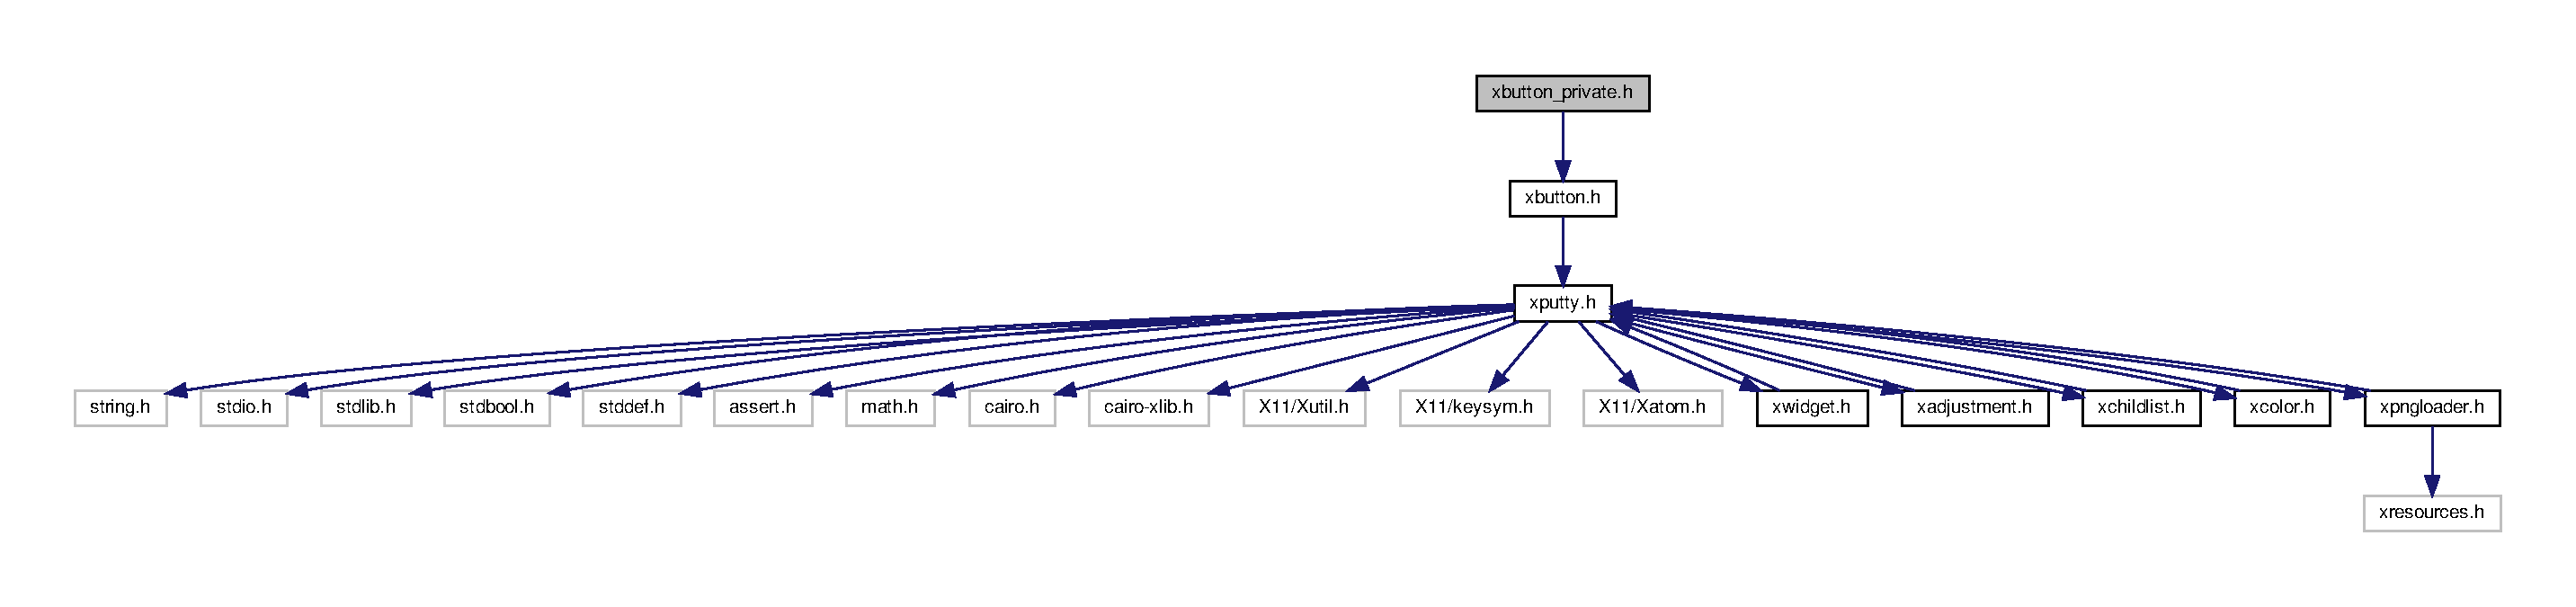
\includegraphics[width=350pt]{xbutton__private_8h__incl}
\end{center}
\end{figure}
This graph shows which files directly or indirectly include this file\+:
\nopagebreak
\begin{figure}[H]
\begin{center}
\leavevmode
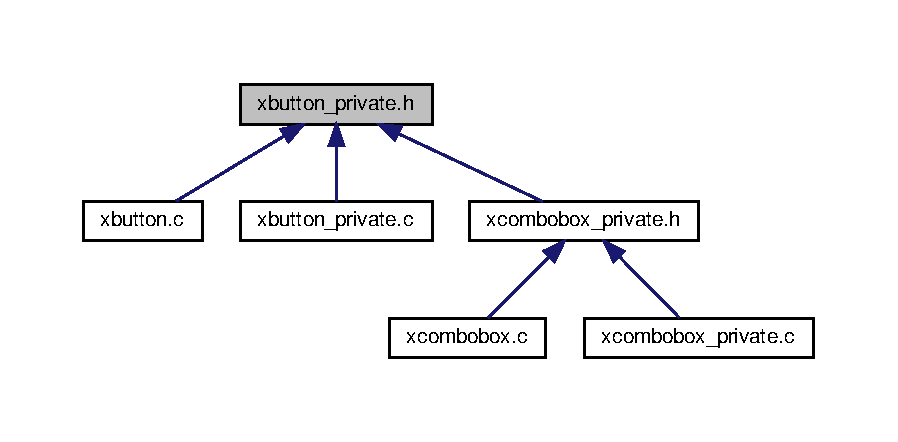
\includegraphics[width=350pt]{xbutton__private_8h__dep__incl}
\end{center}
\end{figure}
\subsection*{Macros}
\begin{DoxyCompactItemize}
\item 
\#define \hyperlink{xbutton__private_8h_a719e82ef2949ca9b4b14413697e85c97}{X\+B\+U\+T\+T\+O\+N\+\_\+\+P\+R\+I\+V\+A\+T\+E\+\_\+\+H\+\_\+}
\end{DoxyCompactItemize}
\subsection*{Functions}
\begin{DoxyCompactItemize}
\item 
void \hyperlink{xbutton__private_8h_ad4e31fc35cac78b036b693d09edfad35}{\+\_\+rounded\+\_\+rectangle} (cairo\+\_\+t $\ast$cr, float x, float y, float width, float height)
\begin{DoxyCompactList}\small\item\em \+\_\+rounded\+\_\+rectangle -\/ internal draw a rounded button \end{DoxyCompactList}\item 
void \hyperlink{xbutton__private_8h_a0ea4425c5e10fa1a3f052afa6114d30b}{\+\_\+pattern\+\_\+out} (\hyperlink{structWidget__t}{Widget\+\_\+t} $\ast$w, \hyperlink{xcolor_8h_af6e1bc675d5df2f7fb9e91a8c5820771}{Color\+\_\+state} st, int height)
\begin{DoxyCompactList}\small\item\em \+\_\+pattern\+\_\+in -\/ a little pattern to make press state more visible \end{DoxyCompactList}\item 
void \hyperlink{xbutton__private_8h_a7b78e740b4f0797a42a53278bfb3c7d4}{\+\_\+pattern\+\_\+in} (\hyperlink{structWidget__t}{Widget\+\_\+t} $\ast$w, \hyperlink{xcolor_8h_af6e1bc675d5df2f7fb9e91a8c5820771}{Color\+\_\+state} st, int height)
\begin{DoxyCompactList}\small\item\em \+\_\+pattern\+\_\+in -\/ a little pattern to make press state more visible \end{DoxyCompactList}\item 
void \hyperlink{xbutton__private_8h_a555079b56b3d52f2a74c20f6ebd05e29}{\+\_\+draw\+\_\+button} (void $\ast$w\+\_\+, void $\ast$user\+\_\+data)
\begin{DoxyCompactList}\small\item\em \+\_\+draw\+\_\+button -\/ internal draw the button to the buffer \end{DoxyCompactList}\item 
void \hyperlink{xbutton__private_8h_abdbb2a0a2e7b10fea4d2147f8ef32248}{\+\_\+draw\+\_\+ti\+\_\+button} (void $\ast$w\+\_\+, void $\ast$user\+\_\+data)
\begin{DoxyCompactList}\small\item\em \+\_\+draw\+\_\+ti\+\_\+button -\/ internal draw the button to the buffer \end{DoxyCompactList}\item 
void \hyperlink{xbutton__private_8h_a4b59433c1a0932889318dcd64943a299}{\+\_\+draw\+\_\+check\+\_\+button} (void $\ast$w\+\_\+, void $\ast$user\+\_\+data)
\begin{DoxyCompactList}\small\item\em \+\_\+draw\+\_\+check\+\_\+button -\/ internal draw the button to the buffer \end{DoxyCompactList}\item 
void \hyperlink{xbutton__private_8h_a9517adc82343f559ff950b4cd632931d}{\+\_\+draw\+\_\+check\+\_\+box} (void $\ast$w\+\_\+, void $\ast$user\+\_\+data)
\begin{DoxyCompactList}\small\item\em \+\_\+draw\+\_\+check\+\_\+box -\/ internal draw the check box to the buffer \end{DoxyCompactList}\item 
void \hyperlink{xbutton__private_8h_a28a4fe06426208c720b93c1fa51aff49}{\+\_\+button\+\_\+pressed} (void $\ast$w\+\_\+, void $\ast$button, void $\ast$user\+\_\+data)
\begin{DoxyCompactList}\small\item\em \+\_\+button\+\_\+pressed -\/ redraw the button and send state via user\+\_\+callback \end{DoxyCompactList}\item 
void \hyperlink{xbutton__private_8h_a0168623590cbb3b5f19ae0878ea41a5f}{\+\_\+button\+\_\+released} (void $\ast$w\+\_\+, void $\ast$button\+\_\+, void $\ast$user\+\_\+data)
\begin{DoxyCompactList}\small\item\em \+\_\+button\+\_\+released -\/ redraw the button and send state via user\+\_\+callback \end{DoxyCompactList}\item 
void \hyperlink{xbutton__private_8h_a31d787399bcdba7f2589a9499d45695f}{\+\_\+toggle\+\_\+button\+\_\+pressed} (void $\ast$w\+\_\+, void $\ast$button, void $\ast$user\+\_\+data)
\begin{DoxyCompactList}\small\item\em \+\_\+toggle\+\_\+button\+\_\+pressed -\/ redraw the button and send state via user\+\_\+callback \end{DoxyCompactList}\item 
void \hyperlink{xbutton__private_8h_a0aed08450617940038e61344f5d67743}{\+\_\+toggle\+\_\+button\+\_\+released} (void $\ast$w\+\_\+, void $\ast$button\+\_\+, void $\ast$user\+\_\+data)
\begin{DoxyCompactList}\small\item\em \+\_\+toggle\+\_\+button\+\_\+released -\/ redraw the button and send state via user\+\_\+callback \end{DoxyCompactList}\end{DoxyCompactItemize}


\subsection{Macro Definition Documentation}
\mbox{\Hypertarget{xbutton__private_8h_a719e82ef2949ca9b4b14413697e85c97}\label{xbutton__private_8h_a719e82ef2949ca9b4b14413697e85c97}} 
\index{xbutton\+\_\+private.\+h@{xbutton\+\_\+private.\+h}!X\+B\+U\+T\+T\+O\+N\+\_\+\+P\+R\+I\+V\+A\+T\+E\+\_\+\+H\+\_\+@{X\+B\+U\+T\+T\+O\+N\+\_\+\+P\+R\+I\+V\+A\+T\+E\+\_\+\+H\+\_\+}}
\index{X\+B\+U\+T\+T\+O\+N\+\_\+\+P\+R\+I\+V\+A\+T\+E\+\_\+\+H\+\_\+@{X\+B\+U\+T\+T\+O\+N\+\_\+\+P\+R\+I\+V\+A\+T\+E\+\_\+\+H\+\_\+}!xbutton\+\_\+private.\+h@{xbutton\+\_\+private.\+h}}
\subsubsection{\texorpdfstring{X\+B\+U\+T\+T\+O\+N\+\_\+\+P\+R\+I\+V\+A\+T\+E\+\_\+\+H\+\_\+}{XBUTTON\_PRIVATE\_H\_}}
{\footnotesize\ttfamily \#define X\+B\+U\+T\+T\+O\+N\+\_\+\+P\+R\+I\+V\+A\+T\+E\+\_\+\+H\+\_\+}



\subsection{Function Documentation}
\mbox{\Hypertarget{xbutton__private_8h_a28a4fe06426208c720b93c1fa51aff49}\label{xbutton__private_8h_a28a4fe06426208c720b93c1fa51aff49}} 
\index{xbutton\+\_\+private.\+h@{xbutton\+\_\+private.\+h}!\+\_\+button\+\_\+pressed@{\+\_\+button\+\_\+pressed}}
\index{\+\_\+button\+\_\+pressed@{\+\_\+button\+\_\+pressed}!xbutton\+\_\+private.\+h@{xbutton\+\_\+private.\+h}}
\subsubsection{\texorpdfstring{\+\_\+button\+\_\+pressed()}{\_button\_pressed()}}
{\footnotesize\ttfamily void \+\_\+button\+\_\+pressed (\begin{DoxyParamCaption}\item[{void $\ast$}]{w\+\_\+,  }\item[{void $\ast$}]{button,  }\item[{void $\ast$}]{user\+\_\+data }\end{DoxyParamCaption})}



\+\_\+button\+\_\+pressed -\/ redraw the button and send state via user\+\_\+callback 


\begin{DoxyParams}{Parameters}
{\em $\ast$w\+\_\+} & -\/ void pointer to the \hyperlink{structWidget__t}{Widget\+\_\+t} button \\
\hline
{\em $\ast$button} & -\/ void pointer to X\+Event.\+xbutton struct \\
\hline
{\em $\ast$user\+\_\+data} & -\/ void pointer to attached user\+\_\+data \\
\hline
\end{DoxyParams}
\begin{DoxyReturn}{Returns}
void 
\end{DoxyReturn}
\mbox{\Hypertarget{xbutton__private_8h_a0168623590cbb3b5f19ae0878ea41a5f}\label{xbutton__private_8h_a0168623590cbb3b5f19ae0878ea41a5f}} 
\index{xbutton\+\_\+private.\+h@{xbutton\+\_\+private.\+h}!\+\_\+button\+\_\+released@{\+\_\+button\+\_\+released}}
\index{\+\_\+button\+\_\+released@{\+\_\+button\+\_\+released}!xbutton\+\_\+private.\+h@{xbutton\+\_\+private.\+h}}
\subsubsection{\texorpdfstring{\+\_\+button\+\_\+released()}{\_button\_released()}}
{\footnotesize\ttfamily void \+\_\+button\+\_\+released (\begin{DoxyParamCaption}\item[{void $\ast$}]{w\+\_\+,  }\item[{void $\ast$}]{button\+\_\+,  }\item[{void $\ast$}]{user\+\_\+data }\end{DoxyParamCaption})}



\+\_\+button\+\_\+released -\/ redraw the button and send state via user\+\_\+callback 


\begin{DoxyParams}{Parameters}
{\em $\ast$w\+\_\+} & -\/ void pointer to the \hyperlink{structWidget__t}{Widget\+\_\+t} button \\
\hline
{\em $\ast$button} & -\/ void pointer to X\+Event.\+xbutton struct \\
\hline
{\em $\ast$user\+\_\+data} & -\/ void pointer to attached user\+\_\+data \\
\hline
\end{DoxyParams}
\begin{DoxyReturn}{Returns}
void 
\end{DoxyReturn}
\mbox{\Hypertarget{xbutton__private_8h_a555079b56b3d52f2a74c20f6ebd05e29}\label{xbutton__private_8h_a555079b56b3d52f2a74c20f6ebd05e29}} 
\index{xbutton\+\_\+private.\+h@{xbutton\+\_\+private.\+h}!\+\_\+draw\+\_\+button@{\+\_\+draw\+\_\+button}}
\index{\+\_\+draw\+\_\+button@{\+\_\+draw\+\_\+button}!xbutton\+\_\+private.\+h@{xbutton\+\_\+private.\+h}}
\subsubsection{\texorpdfstring{\+\_\+draw\+\_\+button()}{\_draw\_button()}}
{\footnotesize\ttfamily void \+\_\+draw\+\_\+button (\begin{DoxyParamCaption}\item[{void $\ast$}]{w\+\_\+,  }\item[{void $\ast$}]{user\+\_\+data }\end{DoxyParamCaption})}



\+\_\+draw\+\_\+button -\/ internal draw the button to the buffer 


\begin{DoxyParams}{Parameters}
{\em $\ast$w\+\_\+} & -\/ void pointer to the \hyperlink{structWidget__t}{Widget\+\_\+t} button \\
\hline
{\em $\ast$user\+\_\+data} & -\/ void pointer to attached user\+\_\+data \\
\hline
\end{DoxyParams}
\begin{DoxyReturn}{Returns}
void 
\end{DoxyReturn}
\mbox{\Hypertarget{xbutton__private_8h_a9517adc82343f559ff950b4cd632931d}\label{xbutton__private_8h_a9517adc82343f559ff950b4cd632931d}} 
\index{xbutton\+\_\+private.\+h@{xbutton\+\_\+private.\+h}!\+\_\+draw\+\_\+check\+\_\+box@{\+\_\+draw\+\_\+check\+\_\+box}}
\index{\+\_\+draw\+\_\+check\+\_\+box@{\+\_\+draw\+\_\+check\+\_\+box}!xbutton\+\_\+private.\+h@{xbutton\+\_\+private.\+h}}
\subsubsection{\texorpdfstring{\+\_\+draw\+\_\+check\+\_\+box()}{\_draw\_check\_box()}}
{\footnotesize\ttfamily void \+\_\+draw\+\_\+check\+\_\+box (\begin{DoxyParamCaption}\item[{void $\ast$}]{w\+\_\+,  }\item[{void $\ast$}]{user\+\_\+data }\end{DoxyParamCaption})}



\+\_\+draw\+\_\+check\+\_\+box -\/ internal draw the check box to the buffer 


\begin{DoxyParams}{Parameters}
{\em $\ast$w\+\_\+} & -\/ void pointer to the \hyperlink{structWidget__t}{Widget\+\_\+t} button \\
\hline
{\em $\ast$user\+\_\+data} & -\/ void pointer to attached user\+\_\+data \\
\hline
\end{DoxyParams}
\begin{DoxyReturn}{Returns}
void 
\end{DoxyReturn}
\mbox{\Hypertarget{xbutton__private_8h_a4b59433c1a0932889318dcd64943a299}\label{xbutton__private_8h_a4b59433c1a0932889318dcd64943a299}} 
\index{xbutton\+\_\+private.\+h@{xbutton\+\_\+private.\+h}!\+\_\+draw\+\_\+check\+\_\+button@{\+\_\+draw\+\_\+check\+\_\+button}}
\index{\+\_\+draw\+\_\+check\+\_\+button@{\+\_\+draw\+\_\+check\+\_\+button}!xbutton\+\_\+private.\+h@{xbutton\+\_\+private.\+h}}
\subsubsection{\texorpdfstring{\+\_\+draw\+\_\+check\+\_\+button()}{\_draw\_check\_button()}}
{\footnotesize\ttfamily void \+\_\+draw\+\_\+check\+\_\+button (\begin{DoxyParamCaption}\item[{void $\ast$}]{w\+\_\+,  }\item[{void $\ast$}]{user\+\_\+data }\end{DoxyParamCaption})}



\+\_\+draw\+\_\+check\+\_\+button -\/ internal draw the button to the buffer 


\begin{DoxyParams}{Parameters}
{\em $\ast$w\+\_\+} & -\/ void pointer to the \hyperlink{structWidget__t}{Widget\+\_\+t} button \\
\hline
{\em $\ast$user\+\_\+data} & -\/ void pointer to attached user\+\_\+data \\
\hline
\end{DoxyParams}
\begin{DoxyReturn}{Returns}
void 
\end{DoxyReturn}
\mbox{\Hypertarget{xbutton__private_8h_abdbb2a0a2e7b10fea4d2147f8ef32248}\label{xbutton__private_8h_abdbb2a0a2e7b10fea4d2147f8ef32248}} 
\index{xbutton\+\_\+private.\+h@{xbutton\+\_\+private.\+h}!\+\_\+draw\+\_\+ti\+\_\+button@{\+\_\+draw\+\_\+ti\+\_\+button}}
\index{\+\_\+draw\+\_\+ti\+\_\+button@{\+\_\+draw\+\_\+ti\+\_\+button}!xbutton\+\_\+private.\+h@{xbutton\+\_\+private.\+h}}
\subsubsection{\texorpdfstring{\+\_\+draw\+\_\+ti\+\_\+button()}{\_draw\_ti\_button()}}
{\footnotesize\ttfamily void \+\_\+draw\+\_\+ti\+\_\+button (\begin{DoxyParamCaption}\item[{void $\ast$}]{w\+\_\+,  }\item[{void $\ast$}]{user\+\_\+data }\end{DoxyParamCaption})}



\+\_\+draw\+\_\+ti\+\_\+button -\/ internal draw the button to the buffer 


\begin{DoxyParams}{Parameters}
{\em $\ast$w\+\_\+} & -\/ void pointer to the \hyperlink{structWidget__t}{Widget\+\_\+t} button \\
\hline
{\em $\ast$user\+\_\+data} & -\/ void pointer to attached user\+\_\+data \\
\hline
\end{DoxyParams}
\begin{DoxyReturn}{Returns}
void 
\end{DoxyReturn}
\mbox{\Hypertarget{xbutton__private_8h_a7b78e740b4f0797a42a53278bfb3c7d4}\label{xbutton__private_8h_a7b78e740b4f0797a42a53278bfb3c7d4}} 
\index{xbutton\+\_\+private.\+h@{xbutton\+\_\+private.\+h}!\+\_\+pattern\+\_\+in@{\+\_\+pattern\+\_\+in}}
\index{\+\_\+pattern\+\_\+in@{\+\_\+pattern\+\_\+in}!xbutton\+\_\+private.\+h@{xbutton\+\_\+private.\+h}}
\subsubsection{\texorpdfstring{\+\_\+pattern\+\_\+in()}{\_pattern\_in()}}
{\footnotesize\ttfamily void \+\_\+pattern\+\_\+in (\begin{DoxyParamCaption}\item[{\hyperlink{structWidget__t}{Widget\+\_\+t} $\ast$}]{w,  }\item[{\hyperlink{xcolor_8h_af6e1bc675d5df2f7fb9e91a8c5820771}{Color\+\_\+state}}]{st,  }\item[{int}]{height }\end{DoxyParamCaption})}



\+\_\+pattern\+\_\+in -\/ a little pattern to make press state more visible 


\begin{DoxyParams}{Parameters}
{\em $\ast$w\+\_\+} & -\/ void pointer to the \hyperlink{structWidget__t}{Widget\+\_\+t} button \\
\hline
{\em st} & -\/ the color state to use \\
\hline
{\em height} & -\/ the button height \\
\hline
\end{DoxyParams}
\begin{DoxyReturn}{Returns}
void 
\end{DoxyReturn}
\mbox{\Hypertarget{xbutton__private_8h_a0ea4425c5e10fa1a3f052afa6114d30b}\label{xbutton__private_8h_a0ea4425c5e10fa1a3f052afa6114d30b}} 
\index{xbutton\+\_\+private.\+h@{xbutton\+\_\+private.\+h}!\+\_\+pattern\+\_\+out@{\+\_\+pattern\+\_\+out}}
\index{\+\_\+pattern\+\_\+out@{\+\_\+pattern\+\_\+out}!xbutton\+\_\+private.\+h@{xbutton\+\_\+private.\+h}}
\subsubsection{\texorpdfstring{\+\_\+pattern\+\_\+out()}{\_pattern\_out()}}
{\footnotesize\ttfamily void \+\_\+pattern\+\_\+out (\begin{DoxyParamCaption}\item[{\hyperlink{structWidget__t}{Widget\+\_\+t} $\ast$}]{w,  }\item[{\hyperlink{xcolor_8h_af6e1bc675d5df2f7fb9e91a8c5820771}{Color\+\_\+state}}]{st,  }\item[{int}]{height }\end{DoxyParamCaption})}



\+\_\+pattern\+\_\+in -\/ a little pattern to make press state more visible 


\begin{DoxyParams}{Parameters}
{\em $\ast$w\+\_\+} & -\/ void pointer to the \hyperlink{structWidget__t}{Widget\+\_\+t} button \\
\hline
{\em st} & -\/ the color state to use \\
\hline
{\em height} & -\/ the button height \\
\hline
\end{DoxyParams}
\begin{DoxyReturn}{Returns}
void 
\end{DoxyReturn}
\mbox{\Hypertarget{xbutton__private_8h_ad4e31fc35cac78b036b693d09edfad35}\label{xbutton__private_8h_ad4e31fc35cac78b036b693d09edfad35}} 
\index{xbutton\+\_\+private.\+h@{xbutton\+\_\+private.\+h}!\+\_\+rounded\+\_\+rectangle@{\+\_\+rounded\+\_\+rectangle}}
\index{\+\_\+rounded\+\_\+rectangle@{\+\_\+rounded\+\_\+rectangle}!xbutton\+\_\+private.\+h@{xbutton\+\_\+private.\+h}}
\subsubsection{\texorpdfstring{\+\_\+rounded\+\_\+rectangle()}{\_rounded\_rectangle()}}
{\footnotesize\ttfamily void \+\_\+rounded\+\_\+rectangle (\begin{DoxyParamCaption}\item[{cairo\+\_\+t $\ast$}]{cr,  }\item[{float}]{x,  }\item[{float}]{y,  }\item[{float}]{width,  }\item[{float}]{height }\end{DoxyParamCaption})}



\+\_\+rounded\+\_\+rectangle -\/ internal draw a rounded button 


\begin{DoxyParams}{Parameters}
{\em x} & -\/ point on x axis \\
\hline
{\em y} & -\/ point on y axis \\
\hline
{\em width} & -\/ the button width \\
\hline
{\em height} & -\/ the button height \\
\hline
\end{DoxyParams}
\begin{DoxyReturn}{Returns}
void 
\end{DoxyReturn}
\mbox{\Hypertarget{xbutton__private_8h_a31d787399bcdba7f2589a9499d45695f}\label{xbutton__private_8h_a31d787399bcdba7f2589a9499d45695f}} 
\index{xbutton\+\_\+private.\+h@{xbutton\+\_\+private.\+h}!\+\_\+toggle\+\_\+button\+\_\+pressed@{\+\_\+toggle\+\_\+button\+\_\+pressed}}
\index{\+\_\+toggle\+\_\+button\+\_\+pressed@{\+\_\+toggle\+\_\+button\+\_\+pressed}!xbutton\+\_\+private.\+h@{xbutton\+\_\+private.\+h}}
\subsubsection{\texorpdfstring{\+\_\+toggle\+\_\+button\+\_\+pressed()}{\_toggle\_button\_pressed()}}
{\footnotesize\ttfamily void \+\_\+toggle\+\_\+button\+\_\+pressed (\begin{DoxyParamCaption}\item[{void $\ast$}]{w\+\_\+,  }\item[{void $\ast$}]{button,  }\item[{void $\ast$}]{user\+\_\+data }\end{DoxyParamCaption})}



\+\_\+toggle\+\_\+button\+\_\+pressed -\/ redraw the button and send state via user\+\_\+callback 


\begin{DoxyParams}{Parameters}
{\em $\ast$w\+\_\+} & -\/ void pointer to the \hyperlink{structWidget__t}{Widget\+\_\+t} button \\
\hline
{\em $\ast$button} & -\/ void pointer to X\+Event.\+xbutton struct \\
\hline
{\em $\ast$user\+\_\+data} & -\/ void pointer to attached user\+\_\+data \\
\hline
\end{DoxyParams}
\begin{DoxyReturn}{Returns}
void 
\end{DoxyReturn}
\mbox{\Hypertarget{xbutton__private_8h_a0aed08450617940038e61344f5d67743}\label{xbutton__private_8h_a0aed08450617940038e61344f5d67743}} 
\index{xbutton\+\_\+private.\+h@{xbutton\+\_\+private.\+h}!\+\_\+toggle\+\_\+button\+\_\+released@{\+\_\+toggle\+\_\+button\+\_\+released}}
\index{\+\_\+toggle\+\_\+button\+\_\+released@{\+\_\+toggle\+\_\+button\+\_\+released}!xbutton\+\_\+private.\+h@{xbutton\+\_\+private.\+h}}
\subsubsection{\texorpdfstring{\+\_\+toggle\+\_\+button\+\_\+released()}{\_toggle\_button\_released()}}
{\footnotesize\ttfamily void \+\_\+toggle\+\_\+button\+\_\+released (\begin{DoxyParamCaption}\item[{void $\ast$}]{w\+\_\+,  }\item[{void $\ast$}]{button\+\_\+,  }\item[{void $\ast$}]{user\+\_\+data }\end{DoxyParamCaption})}



\+\_\+toggle\+\_\+button\+\_\+released -\/ redraw the button and send state via user\+\_\+callback 


\begin{DoxyParams}{Parameters}
{\em $\ast$w\+\_\+} & -\/ void pointer to the \hyperlink{structWidget__t}{Widget\+\_\+t} button \\
\hline
{\em $\ast$button} & -\/ void pointer to X\+Event.\+xbutton struct \\
\hline
{\em $\ast$user\+\_\+data} & -\/ void pointer to attached user\+\_\+data \\
\hline
\end{DoxyParams}
\begin{DoxyReturn}{Returns}
void 
\end{DoxyReturn}

\hypertarget{xchildlist_8c}{}\section{xchildlist.\+c File Reference}
\label{xchildlist_8c}\index{xchildlist.\+c@{xchildlist.\+c}}
{\ttfamily \#include \char`\"{}xchildlist.\+h\char`\"{}}\newline
Include dependency graph for xchildlist.\+c\+:
\nopagebreak
\begin{figure}[H]
\begin{center}
\leavevmode
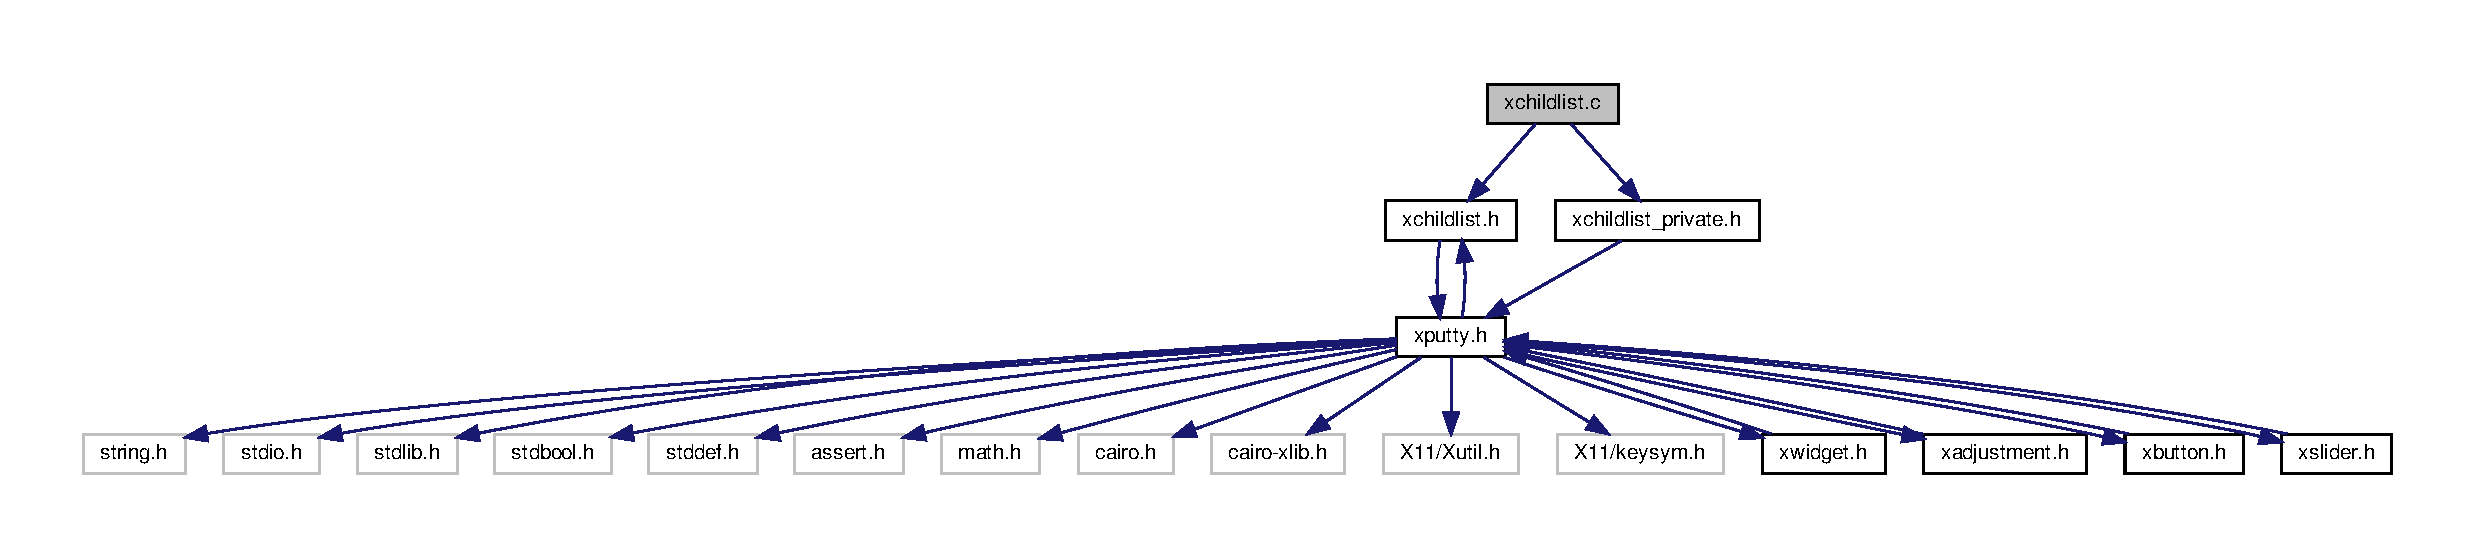
\includegraphics[width=350pt]{xchildlist_8c__incl}
\end{center}
\end{figure}
\subsection*{Functions}
\begin{DoxyCompactItemize}
\item 
void \hyperlink{xchildlist_8c_ad47bf3695fdf0c67bc059e4ce25c4639}{childlist\+\_\+init} (\hyperlink{structChildlist__t}{Childlist\+\_\+t} $\ast$childlist)
\begin{DoxyCompactList}\small\item\em childlist\+\_\+init -\/ allocate the array to min size \end{DoxyCompactList}\item 
void \hyperlink{xchildlist_8c_a57256a97c272561094da1b7ae5c57638}{childlist\+\_\+destroy} (\hyperlink{structChildlist__t}{Childlist\+\_\+t} $\ast$childlist)
\begin{DoxyCompactList}\small\item\em childlist\+\_\+destroy -\/ free the childlist \end{DoxyCompactList}\item 
void \hyperlink{xchildlist_8c_a4515e80317c76cbfa903c50ddfcfbf58}{childlist\+\_\+add\+\_\+child} (\hyperlink{structChildlist__t}{Childlist\+\_\+t} $\ast$childlist, \hyperlink{structWidget__t}{Widget\+\_\+t} $\ast$child)
\begin{DoxyCompactList}\small\item\em childlist\+\_\+add\+\_\+child -\/ add a child to the childlist \end{DoxyCompactList}\item 
void \hyperlink{xchildlist_8c_a6cdf6afd4fdf75550b6aca31ac42379c}{childlist\+\_\+remove\+\_\+child} (\hyperlink{structChildlist__t}{Childlist\+\_\+t} $\ast$childlist, \hyperlink{structWidget__t}{Widget\+\_\+t} $\ast$child)
\begin{DoxyCompactList}\small\item\em childlist\+\_\+add\+\_\+child -\/ remove a child from the childlist \end{DoxyCompactList}\item 
int \hyperlink{xchildlist_8c_a54b8a01a41d48965bd02c5269d0f2103}{childlist\+\_\+find\+\_\+child} (\hyperlink{structChildlist__t}{Childlist\+\_\+t} $\ast$childlist, \hyperlink{structWidget__t}{Widget\+\_\+t} $\ast$child)
\begin{DoxyCompactList}\small\item\em childlist\+\_\+find\+\_\+child -\/ find a child in a the childlist \end{DoxyCompactList}\item 
int \hyperlink{xchildlist_8c_a11e7045a40b8fea2df768b77936f412c}{childlist\+\_\+find\+\_\+widget} (\hyperlink{structChildlist__t}{Childlist\+\_\+t} $\ast$childlist, Window child\+\_\+window, int $\ast$a)
\begin{DoxyCompactList}\small\item\em childlist\+\_\+find\+\_\+widget -\/ find a child \hyperlink{structWidget__t}{Widget\+\_\+t} in a the childlist \end{DoxyCompactList}\item 
int \hyperlink{xchildlist_8c_af130af096a2f8b3a807e7e2dcf0ee6c0}{childlist\+\_\+has\+\_\+child} (\hyperlink{structChildlist__t}{Childlist\+\_\+t} $\ast$childlist)
\begin{DoxyCompactList}\small\item\em childlist\+\_\+has\+\_\+child -\/ check if childlist contain a child \end{DoxyCompactList}\end{DoxyCompactItemize}


\subsection{Function Documentation}
\mbox{\Hypertarget{xchildlist_8c_a4515e80317c76cbfa903c50ddfcfbf58}\label{xchildlist_8c_a4515e80317c76cbfa903c50ddfcfbf58}} 
\index{xchildlist.\+c@{xchildlist.\+c}!childlist\+\_\+add\+\_\+child@{childlist\+\_\+add\+\_\+child}}
\index{childlist\+\_\+add\+\_\+child@{childlist\+\_\+add\+\_\+child}!xchildlist.\+c@{xchildlist.\+c}}
\subsubsection{\texorpdfstring{childlist\+\_\+add\+\_\+child()}{childlist\_add\_child()}}
{\footnotesize\ttfamily void childlist\+\_\+add\+\_\+child (\begin{DoxyParamCaption}\item[{\hyperlink{structChildlist__t}{Childlist\+\_\+t} $\ast$}]{childlist,  }\item[{\hyperlink{structWidget__t}{Widget\+\_\+t} $\ast$}]{child }\end{DoxyParamCaption})}



childlist\+\_\+add\+\_\+child -\/ add a child to the childlist 


\begin{DoxyParams}{Parameters}
{\em $\ast$childlist} & -\/ pointer to the \hyperlink{structChildlist__t}{Childlist\+\_\+t} \\
\hline
{\em $\ast$child} & -\/ pointer to the child to add \\
\hline
\end{DoxyParams}
\begin{DoxyReturn}{Returns}
void 
\end{DoxyReturn}
\mbox{\Hypertarget{xchildlist_8c_a57256a97c272561094da1b7ae5c57638}\label{xchildlist_8c_a57256a97c272561094da1b7ae5c57638}} 
\index{xchildlist.\+c@{xchildlist.\+c}!childlist\+\_\+destroy@{childlist\+\_\+destroy}}
\index{childlist\+\_\+destroy@{childlist\+\_\+destroy}!xchildlist.\+c@{xchildlist.\+c}}
\subsubsection{\texorpdfstring{childlist\+\_\+destroy()}{childlist\_destroy()}}
{\footnotesize\ttfamily void childlist\+\_\+destroy (\begin{DoxyParamCaption}\item[{\hyperlink{structChildlist__t}{Childlist\+\_\+t} $\ast$}]{childlist }\end{DoxyParamCaption})}



childlist\+\_\+destroy -\/ free the childlist 


\begin{DoxyParams}{Parameters}
{\em $\ast$childlist} & -\/ pointer to the \hyperlink{structChildlist__t}{Childlist\+\_\+t} \\
\hline
\end{DoxyParams}
\begin{DoxyReturn}{Returns}
void 
\end{DoxyReturn}
\mbox{\Hypertarget{xchildlist_8c_a54b8a01a41d48965bd02c5269d0f2103}\label{xchildlist_8c_a54b8a01a41d48965bd02c5269d0f2103}} 
\index{xchildlist.\+c@{xchildlist.\+c}!childlist\+\_\+find\+\_\+child@{childlist\+\_\+find\+\_\+child}}
\index{childlist\+\_\+find\+\_\+child@{childlist\+\_\+find\+\_\+child}!xchildlist.\+c@{xchildlist.\+c}}
\subsubsection{\texorpdfstring{childlist\+\_\+find\+\_\+child()}{childlist\_find\_child()}}
{\footnotesize\ttfamily int childlist\+\_\+find\+\_\+child (\begin{DoxyParamCaption}\item[{\hyperlink{structChildlist__t}{Childlist\+\_\+t} $\ast$}]{childlist,  }\item[{\hyperlink{structWidget__t}{Widget\+\_\+t} $\ast$}]{child }\end{DoxyParamCaption})}



childlist\+\_\+find\+\_\+child -\/ find a child in a the childlist 


\begin{DoxyParams}{Parameters}
{\em $\ast$childlist} & -\/ pointer to the \hyperlink{structChildlist__t}{Childlist\+\_\+t} \\
\hline
{\em $\ast$child} & -\/ pointer to the child to find \\
\hline
\end{DoxyParams}
\begin{DoxyReturn}{Returns}
int -\/ return position in childlist or -\/1 
\end{DoxyReturn}
\mbox{\Hypertarget{xchildlist_8c_a11e7045a40b8fea2df768b77936f412c}\label{xchildlist_8c_a11e7045a40b8fea2df768b77936f412c}} 
\index{xchildlist.\+c@{xchildlist.\+c}!childlist\+\_\+find\+\_\+widget@{childlist\+\_\+find\+\_\+widget}}
\index{childlist\+\_\+find\+\_\+widget@{childlist\+\_\+find\+\_\+widget}!xchildlist.\+c@{xchildlist.\+c}}
\subsubsection{\texorpdfstring{childlist\+\_\+find\+\_\+widget()}{childlist\_find\_widget()}}
{\footnotesize\ttfamily int childlist\+\_\+find\+\_\+widget (\begin{DoxyParamCaption}\item[{\hyperlink{structChildlist__t}{Childlist\+\_\+t} $\ast$}]{childlist,  }\item[{Window}]{child\+\_\+window,  }\item[{int $\ast$}]{a }\end{DoxyParamCaption})}



childlist\+\_\+find\+\_\+widget -\/ find a child \hyperlink{structWidget__t}{Widget\+\_\+t} in a the childlist 


\begin{DoxyParams}{Parameters}
{\em $\ast$childlist} & -\/ pointer to the \hyperlink{structChildlist__t}{Childlist\+\_\+t} \\
\hline
{\em child\+\_\+window} & -\/ the window to find the \hyperlink{structWidget__t}{Widget\+\_\+t} for \\
\hline
\end{DoxyParams}
\begin{DoxyReturn}{Returns}
Widget\+\_\+t$\ast$ -\/ return pointer to Wi\+Dget or N\+U\+LL 
\end{DoxyReturn}
\mbox{\Hypertarget{xchildlist_8c_af130af096a2f8b3a807e7e2dcf0ee6c0}\label{xchildlist_8c_af130af096a2f8b3a807e7e2dcf0ee6c0}} 
\index{xchildlist.\+c@{xchildlist.\+c}!childlist\+\_\+has\+\_\+child@{childlist\+\_\+has\+\_\+child}}
\index{childlist\+\_\+has\+\_\+child@{childlist\+\_\+has\+\_\+child}!xchildlist.\+c@{xchildlist.\+c}}
\subsubsection{\texorpdfstring{childlist\+\_\+has\+\_\+child()}{childlist\_has\_child()}}
{\footnotesize\ttfamily int childlist\+\_\+has\+\_\+child (\begin{DoxyParamCaption}\item[{\hyperlink{structChildlist__t}{Childlist\+\_\+t} $\ast$}]{childlist }\end{DoxyParamCaption})}



childlist\+\_\+has\+\_\+child -\/ check if childlist contain a child 


\begin{DoxyParams}{Parameters}
{\em $\ast$childlist} & -\/ pointer to the \hyperlink{structChildlist__t}{Childlist\+\_\+t} \\
\hline
\end{DoxyParams}
\begin{DoxyReturn}{Returns}
int -\/ return element counter value 
\end{DoxyReturn}
\mbox{\Hypertarget{xchildlist_8c_ad47bf3695fdf0c67bc059e4ce25c4639}\label{xchildlist_8c_ad47bf3695fdf0c67bc059e4ce25c4639}} 
\index{xchildlist.\+c@{xchildlist.\+c}!childlist\+\_\+init@{childlist\+\_\+init}}
\index{childlist\+\_\+init@{childlist\+\_\+init}!xchildlist.\+c@{xchildlist.\+c}}
\subsubsection{\texorpdfstring{childlist\+\_\+init()}{childlist\_init()}}
{\footnotesize\ttfamily void childlist\+\_\+init (\begin{DoxyParamCaption}\item[{\hyperlink{structChildlist__t}{Childlist\+\_\+t} $\ast$}]{childlist }\end{DoxyParamCaption})}



childlist\+\_\+init -\/ allocate the array to min size 


\begin{DoxyParams}{Parameters}
{\em $\ast$childlist} & -\/ pointer to the \hyperlink{structChildlist__t}{Childlist\+\_\+t} \\
\hline
\end{DoxyParams}
\begin{DoxyReturn}{Returns}
void 
\end{DoxyReturn}
\mbox{\Hypertarget{xchildlist_8c_a6cdf6afd4fdf75550b6aca31ac42379c}\label{xchildlist_8c_a6cdf6afd4fdf75550b6aca31ac42379c}} 
\index{xchildlist.\+c@{xchildlist.\+c}!childlist\+\_\+remove\+\_\+child@{childlist\+\_\+remove\+\_\+child}}
\index{childlist\+\_\+remove\+\_\+child@{childlist\+\_\+remove\+\_\+child}!xchildlist.\+c@{xchildlist.\+c}}
\subsubsection{\texorpdfstring{childlist\+\_\+remove\+\_\+child()}{childlist\_remove\_child()}}
{\footnotesize\ttfamily void childlist\+\_\+remove\+\_\+child (\begin{DoxyParamCaption}\item[{\hyperlink{structChildlist__t}{Childlist\+\_\+t} $\ast$}]{childlist,  }\item[{\hyperlink{structWidget__t}{Widget\+\_\+t} $\ast$}]{child }\end{DoxyParamCaption})}



childlist\+\_\+add\+\_\+child -\/ remove a child from the childlist 


\begin{DoxyParams}{Parameters}
{\em $\ast$childlist} & -\/ pointer to the \hyperlink{structChildlist__t}{Childlist\+\_\+t} \\
\hline
{\em $\ast$child} & -\/ pointer to the child to remove \\
\hline
\end{DoxyParams}
\begin{DoxyReturn}{Returns}
void 
\end{DoxyReturn}

\hypertarget{xchildlist_8h}{}\section{xchildlist.\+h File Reference}
\label{xchildlist_8h}\index{xchildlist.\+h@{xchildlist.\+h}}
{\ttfamily \#include \char`\"{}xputty.\+h\char`\"{}}\newline
Include dependency graph for xchildlist.\+h\+:
\nopagebreak
\begin{figure}[H]
\begin{center}
\leavevmode
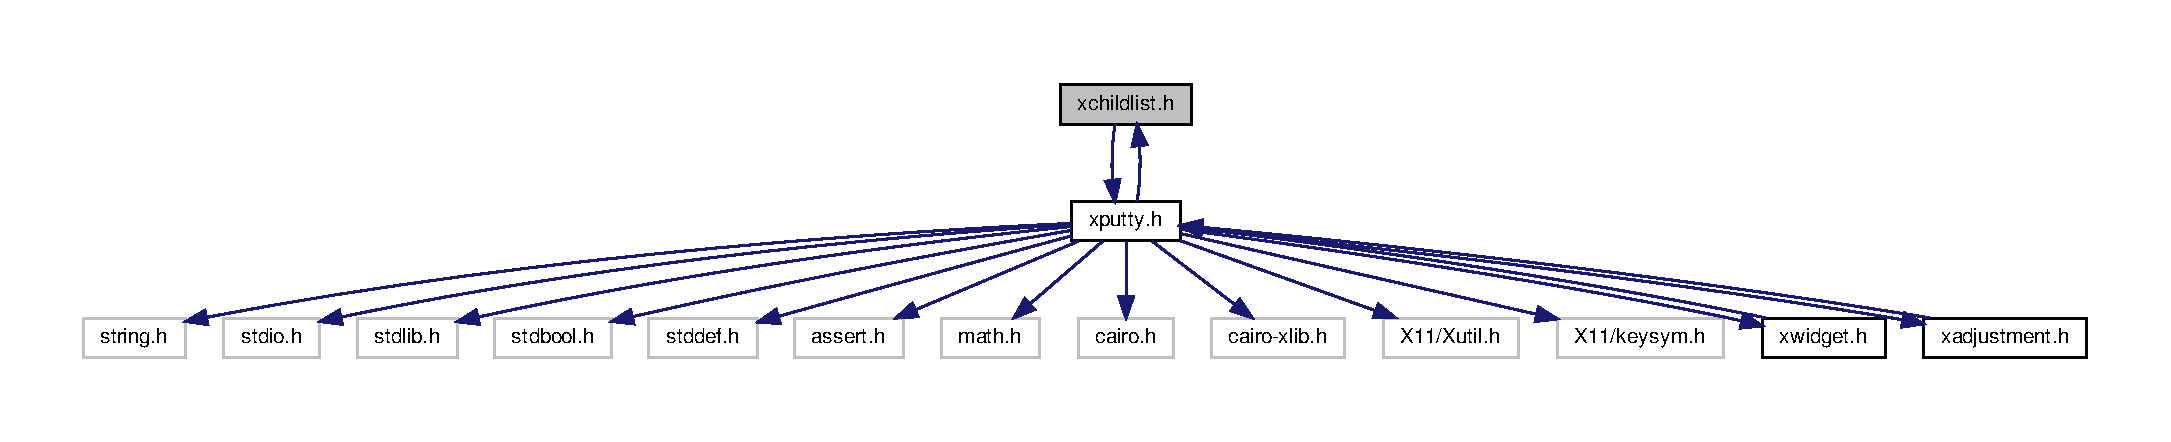
\includegraphics[width=350pt]{xchildlist_8h__incl}
\end{center}
\end{figure}
This graph shows which files directly or indirectly include this file\+:
\nopagebreak
\begin{figure}[H]
\begin{center}
\leavevmode
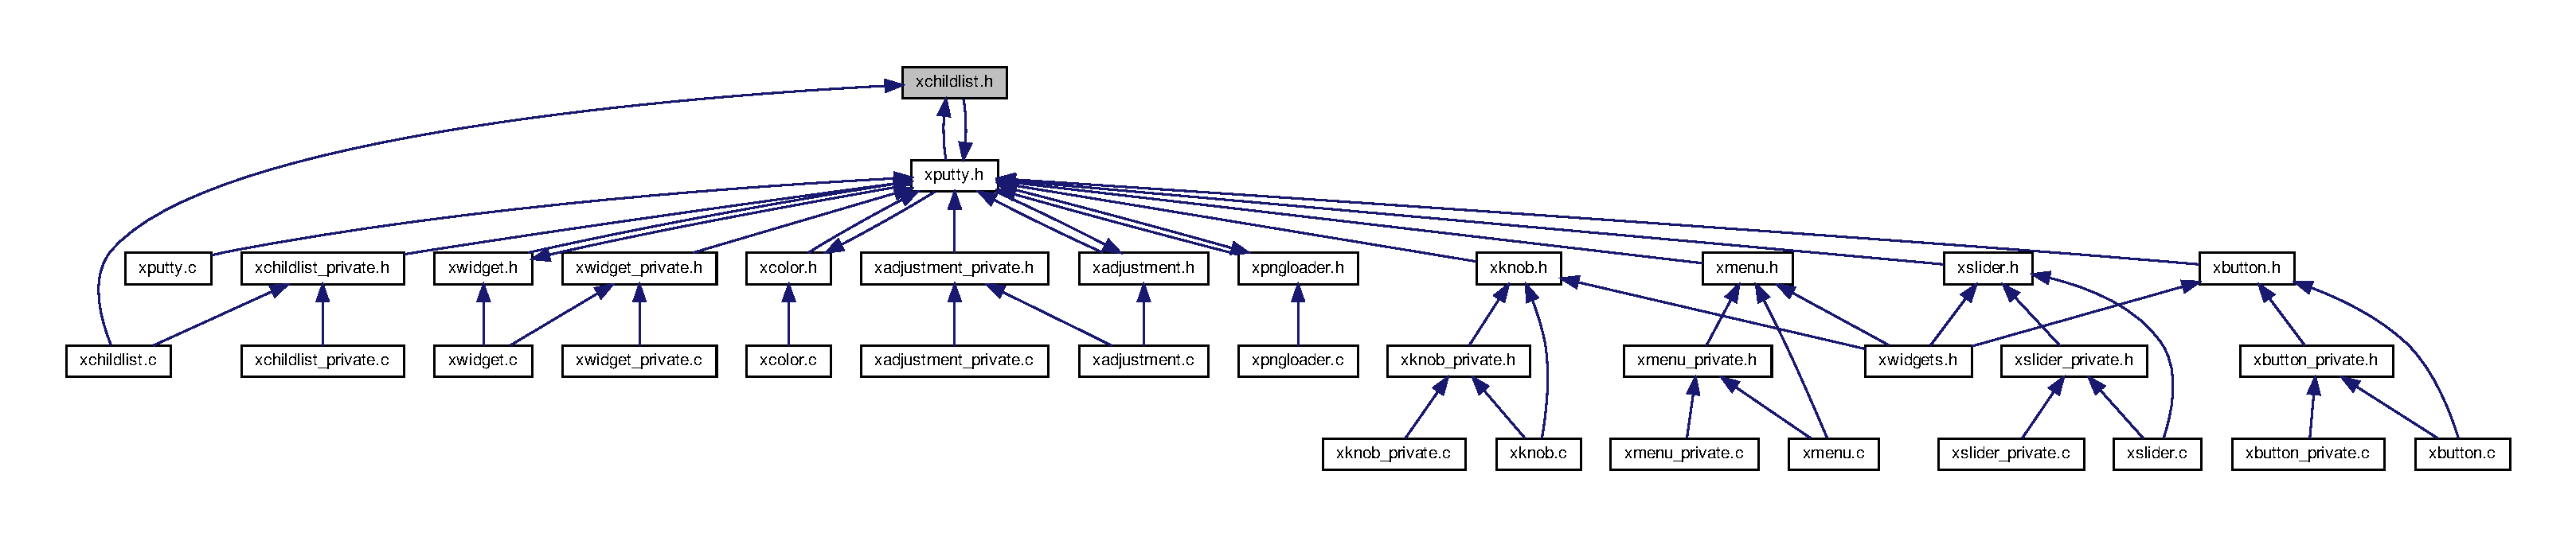
\includegraphics[width=306pt]{xchildlist_8h__dep__incl}
\end{center}
\end{figure}
\subsection*{Data Structures}
\begin{DoxyCompactItemize}
\item 
struct \hyperlink{structChildlist__t}{Childlist\+\_\+t}
\begin{DoxyCompactList}\small\item\em \hyperlink{structChildlist__t}{Childlist\+\_\+t} -\/ struct to hold a \hyperlink{structWidget__t}{Widget\+\_\+t} child list. \end{DoxyCompactList}\end{DoxyCompactItemize}
\subsection*{Macros}
\begin{DoxyCompactItemize}
\item 
\#define \hyperlink{xchildlist_8h_a396cfc2326c57bf038fc8b40d1fc7630}{X\+C\+H\+I\+L\+D\+L\+I\+S\+T\+\_\+\+H\+\_\+}
\end{DoxyCompactItemize}
\subsection*{Functions}
\begin{DoxyCompactItemize}
\item 
void \hyperlink{xchildlist_8h_ad47bf3695fdf0c67bc059e4ce25c4639}{childlist\+\_\+init} (\hyperlink{structChildlist__t}{Childlist\+\_\+t} $\ast$childlist)
\begin{DoxyCompactList}\small\item\em childlist\+\_\+init -\/ allocate the array to min size \end{DoxyCompactList}\item 
void \hyperlink{xchildlist_8h_a57256a97c272561094da1b7ae5c57638}{childlist\+\_\+destroy} (\hyperlink{structChildlist__t}{Childlist\+\_\+t} $\ast$childlist)
\begin{DoxyCompactList}\small\item\em childlist\+\_\+destroy -\/ free the childlist \end{DoxyCompactList}\item 
void \hyperlink{xchildlist_8h_a4515e80317c76cbfa903c50ddfcfbf58}{childlist\+\_\+add\+\_\+child} (\hyperlink{structChildlist__t}{Childlist\+\_\+t} $\ast$childlist, \hyperlink{structWidget__t}{Widget\+\_\+t} $\ast$child)
\begin{DoxyCompactList}\small\item\em childlist\+\_\+add\+\_\+child -\/ add a child to the childlist \end{DoxyCompactList}\item 
void \hyperlink{xchildlist_8h_a6cdf6afd4fdf75550b6aca31ac42379c}{childlist\+\_\+remove\+\_\+child} (\hyperlink{structChildlist__t}{Childlist\+\_\+t} $\ast$childlist, \hyperlink{structWidget__t}{Widget\+\_\+t} $\ast$child)
\begin{DoxyCompactList}\small\item\em childlist\+\_\+add\+\_\+child -\/ remove a child from the childlist \end{DoxyCompactList}\item 
int \hyperlink{xchildlist_8h_a54b8a01a41d48965bd02c5269d0f2103}{childlist\+\_\+find\+\_\+child} (\hyperlink{structChildlist__t}{Childlist\+\_\+t} $\ast$childlist, \hyperlink{structWidget__t}{Widget\+\_\+t} $\ast$child)
\begin{DoxyCompactList}\small\item\em childlist\+\_\+find\+\_\+child -\/ find a child in a the childlist \end{DoxyCompactList}\item 
int \hyperlink{xchildlist_8h_a11e7045a40b8fea2df768b77936f412c}{childlist\+\_\+find\+\_\+widget} (\hyperlink{structChildlist__t}{Childlist\+\_\+t} $\ast$childlist, Window child\+\_\+window, int $\ast$a)
\begin{DoxyCompactList}\small\item\em childlist\+\_\+find\+\_\+widget -\/ find a child \hyperlink{structWidget__t}{Widget\+\_\+t} in a the childlist \end{DoxyCompactList}\item 
int \hyperlink{xchildlist_8h_af130af096a2f8b3a807e7e2dcf0ee6c0}{childlist\+\_\+has\+\_\+child} (\hyperlink{structChildlist__t}{Childlist\+\_\+t} $\ast$childlist)
\begin{DoxyCompactList}\small\item\em childlist\+\_\+has\+\_\+child -\/ check if childlist contain a child \end{DoxyCompactList}\end{DoxyCompactItemize}


\subsection{Macro Definition Documentation}
\mbox{\Hypertarget{xchildlist_8h_a396cfc2326c57bf038fc8b40d1fc7630}\label{xchildlist_8h_a396cfc2326c57bf038fc8b40d1fc7630}} 
\index{xchildlist.\+h@{xchildlist.\+h}!X\+C\+H\+I\+L\+D\+L\+I\+S\+T\+\_\+\+H\+\_\+@{X\+C\+H\+I\+L\+D\+L\+I\+S\+T\+\_\+\+H\+\_\+}}
\index{X\+C\+H\+I\+L\+D\+L\+I\+S\+T\+\_\+\+H\+\_\+@{X\+C\+H\+I\+L\+D\+L\+I\+S\+T\+\_\+\+H\+\_\+}!xchildlist.\+h@{xchildlist.\+h}}
\subsubsection{\texorpdfstring{X\+C\+H\+I\+L\+D\+L\+I\+S\+T\+\_\+\+H\+\_\+}{XCHILDLIST\_H\_}}
{\footnotesize\ttfamily \#define X\+C\+H\+I\+L\+D\+L\+I\+S\+T\+\_\+\+H\+\_\+}



\subsection{Function Documentation}
\mbox{\Hypertarget{xchildlist_8h_a4515e80317c76cbfa903c50ddfcfbf58}\label{xchildlist_8h_a4515e80317c76cbfa903c50ddfcfbf58}} 
\index{xchildlist.\+h@{xchildlist.\+h}!childlist\+\_\+add\+\_\+child@{childlist\+\_\+add\+\_\+child}}
\index{childlist\+\_\+add\+\_\+child@{childlist\+\_\+add\+\_\+child}!xchildlist.\+h@{xchildlist.\+h}}
\subsubsection{\texorpdfstring{childlist\+\_\+add\+\_\+child()}{childlist\_add\_child()}}
{\footnotesize\ttfamily void childlist\+\_\+add\+\_\+child (\begin{DoxyParamCaption}\item[{\hyperlink{structChildlist__t}{Childlist\+\_\+t} $\ast$}]{childlist,  }\item[{\hyperlink{structWidget__t}{Widget\+\_\+t} $\ast$}]{child }\end{DoxyParamCaption})}



childlist\+\_\+add\+\_\+child -\/ add a child to the childlist 


\begin{DoxyParams}{Parameters}
{\em $\ast$childlist} & -\/ pointer to the \hyperlink{structChildlist__t}{Childlist\+\_\+t} \\
\hline
{\em $\ast$child} & -\/ pointer to the child to add \\
\hline
\end{DoxyParams}
\begin{DoxyReturn}{Returns}
void 
\end{DoxyReturn}
\mbox{\Hypertarget{xchildlist_8h_a57256a97c272561094da1b7ae5c57638}\label{xchildlist_8h_a57256a97c272561094da1b7ae5c57638}} 
\index{xchildlist.\+h@{xchildlist.\+h}!childlist\+\_\+destroy@{childlist\+\_\+destroy}}
\index{childlist\+\_\+destroy@{childlist\+\_\+destroy}!xchildlist.\+h@{xchildlist.\+h}}
\subsubsection{\texorpdfstring{childlist\+\_\+destroy()}{childlist\_destroy()}}
{\footnotesize\ttfamily void childlist\+\_\+destroy (\begin{DoxyParamCaption}\item[{\hyperlink{structChildlist__t}{Childlist\+\_\+t} $\ast$}]{childlist }\end{DoxyParamCaption})}



childlist\+\_\+destroy -\/ free the childlist 


\begin{DoxyParams}{Parameters}
{\em $\ast$childlist} & -\/ pointer to the \hyperlink{structChildlist__t}{Childlist\+\_\+t} \\
\hline
\end{DoxyParams}
\begin{DoxyReturn}{Returns}
void 
\end{DoxyReturn}
\mbox{\Hypertarget{xchildlist_8h_a54b8a01a41d48965bd02c5269d0f2103}\label{xchildlist_8h_a54b8a01a41d48965bd02c5269d0f2103}} 
\index{xchildlist.\+h@{xchildlist.\+h}!childlist\+\_\+find\+\_\+child@{childlist\+\_\+find\+\_\+child}}
\index{childlist\+\_\+find\+\_\+child@{childlist\+\_\+find\+\_\+child}!xchildlist.\+h@{xchildlist.\+h}}
\subsubsection{\texorpdfstring{childlist\+\_\+find\+\_\+child()}{childlist\_find\_child()}}
{\footnotesize\ttfamily int childlist\+\_\+find\+\_\+child (\begin{DoxyParamCaption}\item[{\hyperlink{structChildlist__t}{Childlist\+\_\+t} $\ast$}]{childlist,  }\item[{\hyperlink{structWidget__t}{Widget\+\_\+t} $\ast$}]{child }\end{DoxyParamCaption})}



childlist\+\_\+find\+\_\+child -\/ find a child in a the childlist 


\begin{DoxyParams}{Parameters}
{\em $\ast$childlist} & -\/ pointer to the \hyperlink{structChildlist__t}{Childlist\+\_\+t} \\
\hline
{\em $\ast$child} & -\/ pointer to the child to find \\
\hline
\end{DoxyParams}
\begin{DoxyReturn}{Returns}
int -\/ return position in childlist or -\/1 
\end{DoxyReturn}
\mbox{\Hypertarget{xchildlist_8h_a11e7045a40b8fea2df768b77936f412c}\label{xchildlist_8h_a11e7045a40b8fea2df768b77936f412c}} 
\index{xchildlist.\+h@{xchildlist.\+h}!childlist\+\_\+find\+\_\+widget@{childlist\+\_\+find\+\_\+widget}}
\index{childlist\+\_\+find\+\_\+widget@{childlist\+\_\+find\+\_\+widget}!xchildlist.\+h@{xchildlist.\+h}}
\subsubsection{\texorpdfstring{childlist\+\_\+find\+\_\+widget()}{childlist\_find\_widget()}}
{\footnotesize\ttfamily int childlist\+\_\+find\+\_\+widget (\begin{DoxyParamCaption}\item[{\hyperlink{structChildlist__t}{Childlist\+\_\+t} $\ast$}]{childlist,  }\item[{Window}]{child\+\_\+window,  }\item[{int $\ast$}]{a }\end{DoxyParamCaption})}



childlist\+\_\+find\+\_\+widget -\/ find a child \hyperlink{structWidget__t}{Widget\+\_\+t} in a the childlist 


\begin{DoxyParams}{Parameters}
{\em $\ast$childlist} & -\/ pointer to the \hyperlink{structChildlist__t}{Childlist\+\_\+t} \\
\hline
{\em child\+\_\+window} & -\/ the window to find the \hyperlink{structWidget__t}{Widget\+\_\+t} for \\
\hline
\end{DoxyParams}
\begin{DoxyReturn}{Returns}
Widget\+\_\+t$\ast$ -\/ return pointer to Wi\+Dget or N\+U\+LL 
\end{DoxyReturn}
\mbox{\Hypertarget{xchildlist_8h_af130af096a2f8b3a807e7e2dcf0ee6c0}\label{xchildlist_8h_af130af096a2f8b3a807e7e2dcf0ee6c0}} 
\index{xchildlist.\+h@{xchildlist.\+h}!childlist\+\_\+has\+\_\+child@{childlist\+\_\+has\+\_\+child}}
\index{childlist\+\_\+has\+\_\+child@{childlist\+\_\+has\+\_\+child}!xchildlist.\+h@{xchildlist.\+h}}
\subsubsection{\texorpdfstring{childlist\+\_\+has\+\_\+child()}{childlist\_has\_child()}}
{\footnotesize\ttfamily int childlist\+\_\+has\+\_\+child (\begin{DoxyParamCaption}\item[{\hyperlink{structChildlist__t}{Childlist\+\_\+t} $\ast$}]{childlist }\end{DoxyParamCaption})}



childlist\+\_\+has\+\_\+child -\/ check if childlist contain a child 


\begin{DoxyParams}{Parameters}
{\em $\ast$childlist} & -\/ pointer to the \hyperlink{structChildlist__t}{Childlist\+\_\+t} \\
\hline
\end{DoxyParams}
\begin{DoxyReturn}{Returns}
int -\/ return element counter value 
\end{DoxyReturn}
\mbox{\Hypertarget{xchildlist_8h_ad47bf3695fdf0c67bc059e4ce25c4639}\label{xchildlist_8h_ad47bf3695fdf0c67bc059e4ce25c4639}} 
\index{xchildlist.\+h@{xchildlist.\+h}!childlist\+\_\+init@{childlist\+\_\+init}}
\index{childlist\+\_\+init@{childlist\+\_\+init}!xchildlist.\+h@{xchildlist.\+h}}
\subsubsection{\texorpdfstring{childlist\+\_\+init()}{childlist\_init()}}
{\footnotesize\ttfamily void childlist\+\_\+init (\begin{DoxyParamCaption}\item[{\hyperlink{structChildlist__t}{Childlist\+\_\+t} $\ast$}]{childlist }\end{DoxyParamCaption})}



childlist\+\_\+init -\/ allocate the array to min size 


\begin{DoxyParams}{Parameters}
{\em $\ast$childlist} & -\/ pointer to the \hyperlink{structChildlist__t}{Childlist\+\_\+t} \\
\hline
\end{DoxyParams}
\begin{DoxyReturn}{Returns}
void 
\end{DoxyReturn}
\mbox{\Hypertarget{xchildlist_8h_a6cdf6afd4fdf75550b6aca31ac42379c}\label{xchildlist_8h_a6cdf6afd4fdf75550b6aca31ac42379c}} 
\index{xchildlist.\+h@{xchildlist.\+h}!childlist\+\_\+remove\+\_\+child@{childlist\+\_\+remove\+\_\+child}}
\index{childlist\+\_\+remove\+\_\+child@{childlist\+\_\+remove\+\_\+child}!xchildlist.\+h@{xchildlist.\+h}}
\subsubsection{\texorpdfstring{childlist\+\_\+remove\+\_\+child()}{childlist\_remove\_child()}}
{\footnotesize\ttfamily void childlist\+\_\+remove\+\_\+child (\begin{DoxyParamCaption}\item[{\hyperlink{structChildlist__t}{Childlist\+\_\+t} $\ast$}]{childlist,  }\item[{\hyperlink{structWidget__t}{Widget\+\_\+t} $\ast$}]{child }\end{DoxyParamCaption})}



childlist\+\_\+add\+\_\+child -\/ remove a child from the childlist 


\begin{DoxyParams}{Parameters}
{\em $\ast$childlist} & -\/ pointer to the \hyperlink{structChildlist__t}{Childlist\+\_\+t} \\
\hline
{\em $\ast$child} & -\/ pointer to the child to remove \\
\hline
\end{DoxyParams}
\begin{DoxyReturn}{Returns}
void 
\end{DoxyReturn}

\hypertarget{xchildlist__private_8c}{}\section{xchildlist\+\_\+private.\+c File Reference}
\label{xchildlist__private_8c}\index{xchildlist\+\_\+private.\+c@{xchildlist\+\_\+private.\+c}}
{\ttfamily \#include \char`\"{}xchildlist\+\_\+private.\+h\char`\"{}}\newline
Include dependency graph for xchildlist\+\_\+private.\+c\+:
\nopagebreak
\begin{figure}[H]
\begin{center}
\leavevmode
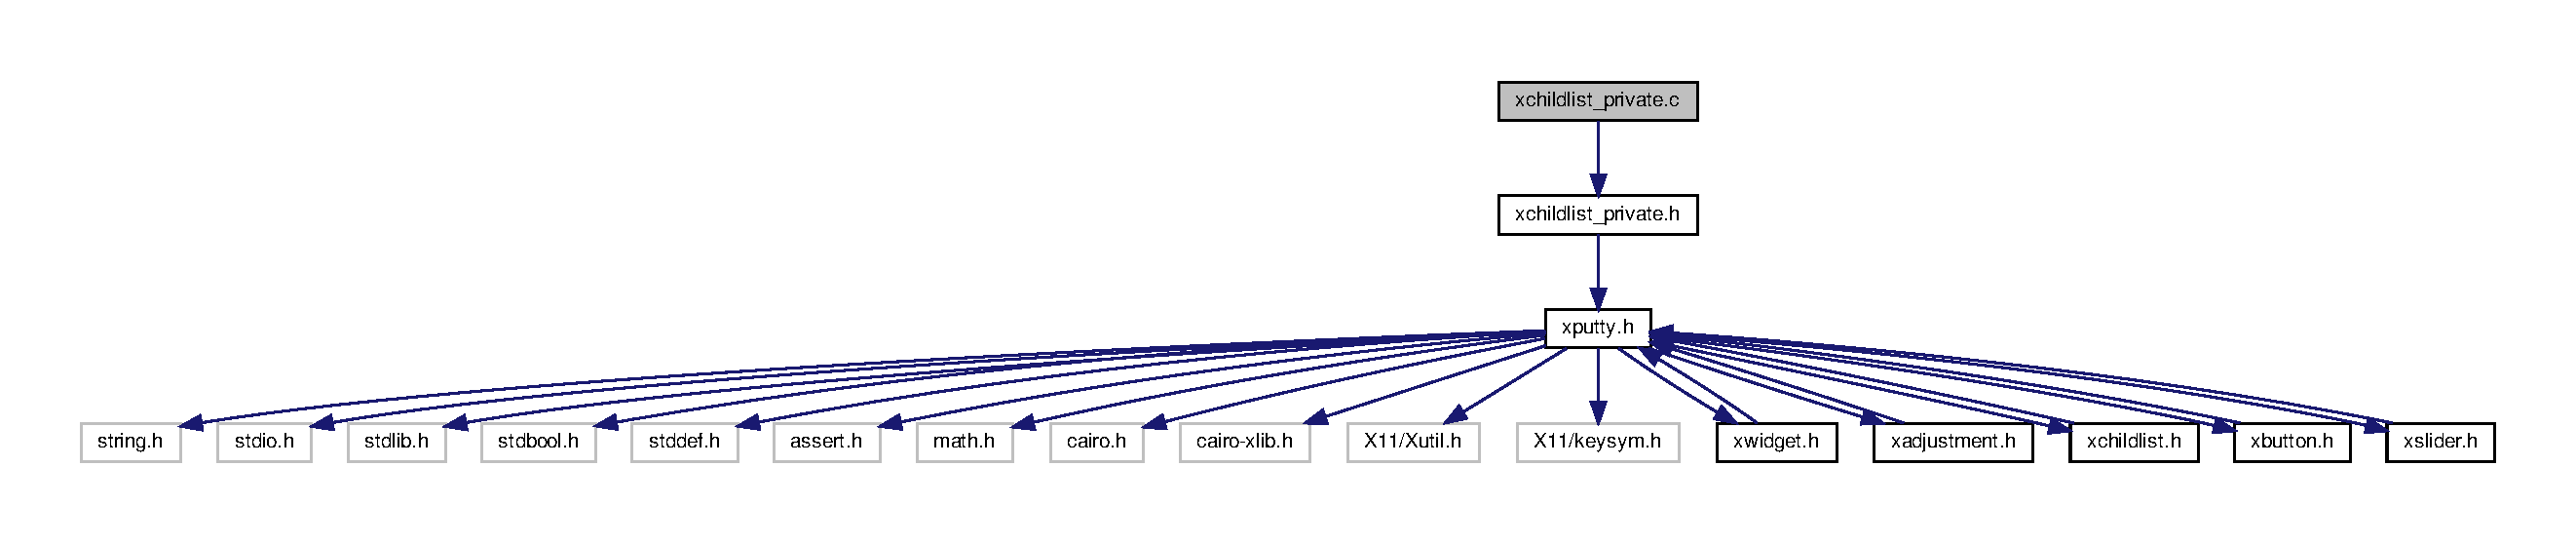
\includegraphics[width=350pt]{xchildlist__private_8c__incl}
\end{center}
\end{figure}
\subsection*{Functions}
\begin{DoxyCompactItemize}
\item 
void \hyperlink{xchildlist__private_8c_a4417a26df5d336bfff97d4210e0291fe}{\+\_\+childlist\+\_\+add\+\_\+elem} (\hyperlink{structChildlist__t}{Childlist\+\_\+t} $\ast$childlist)
\begin{DoxyCompactList}\small\item\em \+\_\+childlist\+\_\+add\+\_\+elem -\/ reallocate the childlist array to new size \end{DoxyCompactList}\end{DoxyCompactItemize}


\subsection{Function Documentation}
\mbox{\Hypertarget{xchildlist__private_8c_a4417a26df5d336bfff97d4210e0291fe}\label{xchildlist__private_8c_a4417a26df5d336bfff97d4210e0291fe}} 
\index{xchildlist\+\_\+private.\+c@{xchildlist\+\_\+private.\+c}!\+\_\+childlist\+\_\+add\+\_\+elem@{\+\_\+childlist\+\_\+add\+\_\+elem}}
\index{\+\_\+childlist\+\_\+add\+\_\+elem@{\+\_\+childlist\+\_\+add\+\_\+elem}!xchildlist\+\_\+private.\+c@{xchildlist\+\_\+private.\+c}}
\subsubsection{\texorpdfstring{\+\_\+childlist\+\_\+add\+\_\+elem()}{\_childlist\_add\_elem()}}
{\footnotesize\ttfamily void \+\_\+childlist\+\_\+add\+\_\+elem (\begin{DoxyParamCaption}\item[{\hyperlink{structChildlist__t}{Childlist\+\_\+t} $\ast$}]{childlist }\end{DoxyParamCaption})}



\+\_\+childlist\+\_\+add\+\_\+elem -\/ reallocate the childlist array to new size 


\begin{DoxyParams}{Parameters}
{\em $\ast$childlist} & -\/ pointer to the \hyperlink{structChildlist__t}{Childlist\+\_\+t} \\
\hline
\end{DoxyParams}
\begin{DoxyReturn}{Returns}
void 
\end{DoxyReturn}

\hypertarget{xchildlist__private_8h}{}\section{xchildlist\+\_\+private.\+h File Reference}
\label{xchildlist__private_8h}\index{xchildlist\+\_\+private.\+h@{xchildlist\+\_\+private.\+h}}
{\ttfamily \#include \char`\"{}xputty.\+h\char`\"{}}\newline
Include dependency graph for xchildlist\+\_\+private.\+h\+:
\nopagebreak
\begin{figure}[H]
\begin{center}
\leavevmode
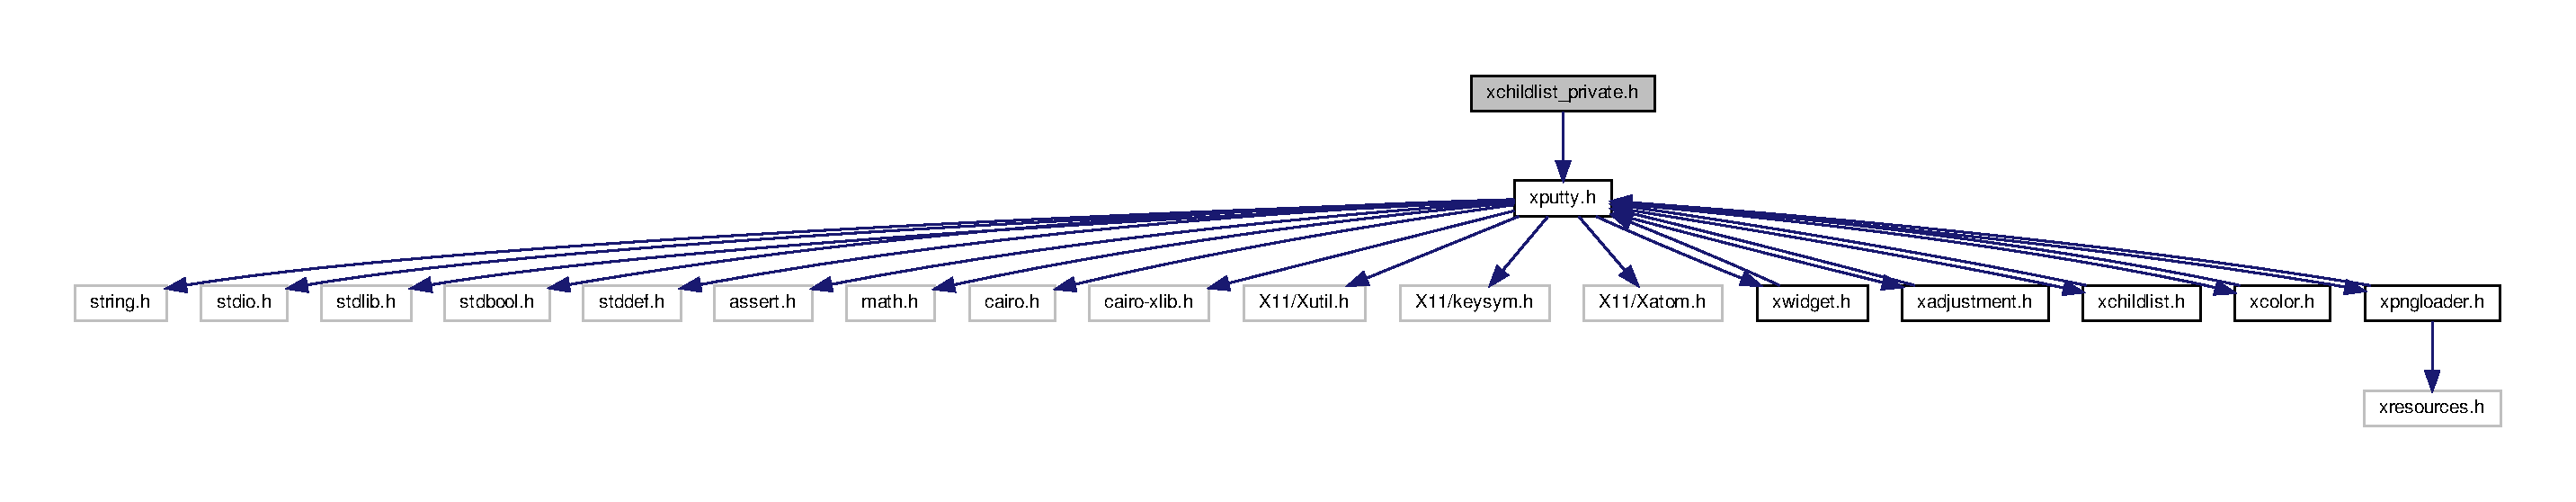
\includegraphics[width=350pt]{xchildlist__private_8h__incl}
\end{center}
\end{figure}
This graph shows which files directly or indirectly include this file\+:
\nopagebreak
\begin{figure}[H]
\begin{center}
\leavevmode
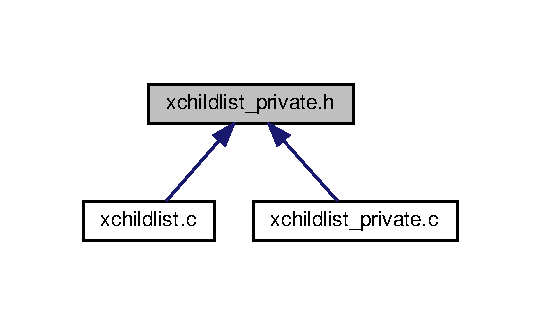
\includegraphics[width=260pt]{xchildlist__private_8h__dep__incl}
\end{center}
\end{figure}
\subsection*{Macros}
\begin{DoxyCompactItemize}
\item 
\#define \hyperlink{xchildlist__private_8h_a60bfdfb9d36bb59620e186c0201ece15}{X\+C\+H\+I\+L\+D\+L\+I\+S\+T\+\_\+\+P\+R\+I\+V\+A\+T\+E\+\_\+\+H\+\_\+}
\end{DoxyCompactItemize}
\subsection*{Functions}
\begin{DoxyCompactItemize}
\item 
void \hyperlink{xchildlist__private_8h_a4417a26df5d336bfff97d4210e0291fe}{\+\_\+childlist\+\_\+add\+\_\+elem} (\hyperlink{structChildlist__t}{Childlist\+\_\+t} $\ast$childlist)
\begin{DoxyCompactList}\small\item\em \+\_\+childlist\+\_\+add\+\_\+elem -\/ reallocate the childlist array to new size \end{DoxyCompactList}\end{DoxyCompactItemize}


\subsection{Macro Definition Documentation}
\mbox{\Hypertarget{xchildlist__private_8h_a60bfdfb9d36bb59620e186c0201ece15}\label{xchildlist__private_8h_a60bfdfb9d36bb59620e186c0201ece15}} 
\index{xchildlist\+\_\+private.\+h@{xchildlist\+\_\+private.\+h}!X\+C\+H\+I\+L\+D\+L\+I\+S\+T\+\_\+\+P\+R\+I\+V\+A\+T\+E\+\_\+\+H\+\_\+@{X\+C\+H\+I\+L\+D\+L\+I\+S\+T\+\_\+\+P\+R\+I\+V\+A\+T\+E\+\_\+\+H\+\_\+}}
\index{X\+C\+H\+I\+L\+D\+L\+I\+S\+T\+\_\+\+P\+R\+I\+V\+A\+T\+E\+\_\+\+H\+\_\+@{X\+C\+H\+I\+L\+D\+L\+I\+S\+T\+\_\+\+P\+R\+I\+V\+A\+T\+E\+\_\+\+H\+\_\+}!xchildlist\+\_\+private.\+h@{xchildlist\+\_\+private.\+h}}
\subsubsection{\texorpdfstring{X\+C\+H\+I\+L\+D\+L\+I\+S\+T\+\_\+\+P\+R\+I\+V\+A\+T\+E\+\_\+\+H\+\_\+}{XCHILDLIST\_PRIVATE\_H\_}}
{\footnotesize\ttfamily \#define X\+C\+H\+I\+L\+D\+L\+I\+S\+T\+\_\+\+P\+R\+I\+V\+A\+T\+E\+\_\+\+H\+\_\+}

here are the private functions from xchildlist 

\subsection{Function Documentation}
\mbox{\Hypertarget{xchildlist__private_8h_a4417a26df5d336bfff97d4210e0291fe}\label{xchildlist__private_8h_a4417a26df5d336bfff97d4210e0291fe}} 
\index{xchildlist\+\_\+private.\+h@{xchildlist\+\_\+private.\+h}!\+\_\+childlist\+\_\+add\+\_\+elem@{\+\_\+childlist\+\_\+add\+\_\+elem}}
\index{\+\_\+childlist\+\_\+add\+\_\+elem@{\+\_\+childlist\+\_\+add\+\_\+elem}!xchildlist\+\_\+private.\+h@{xchildlist\+\_\+private.\+h}}
\subsubsection{\texorpdfstring{\+\_\+childlist\+\_\+add\+\_\+elem()}{\_childlist\_add\_elem()}}
{\footnotesize\ttfamily void \+\_\+childlist\+\_\+add\+\_\+elem (\begin{DoxyParamCaption}\item[{\hyperlink{structChildlist__t}{Childlist\+\_\+t} $\ast$}]{childlist }\end{DoxyParamCaption})}



\+\_\+childlist\+\_\+add\+\_\+elem -\/ reallocate the childlist array to new size 


\begin{DoxyParams}{Parameters}
{\em $\ast$childlist} & -\/ pointer to the \hyperlink{structChildlist__t}{Childlist\+\_\+t} \\
\hline
\end{DoxyParams}
\begin{DoxyReturn}{Returns}
void 
\end{DoxyReturn}

\hypertarget{xputty_8c}{}\section{xputty.\+c File Reference}
\label{xputty_8c}\index{xputty.\+c@{xputty.\+c}}
{\ttfamily \#include \char`\"{}xputty.\+h\char`\"{}}\newline
Include dependency graph for xputty.\+c\+:
\nopagebreak
\begin{figure}[H]
\begin{center}
\leavevmode
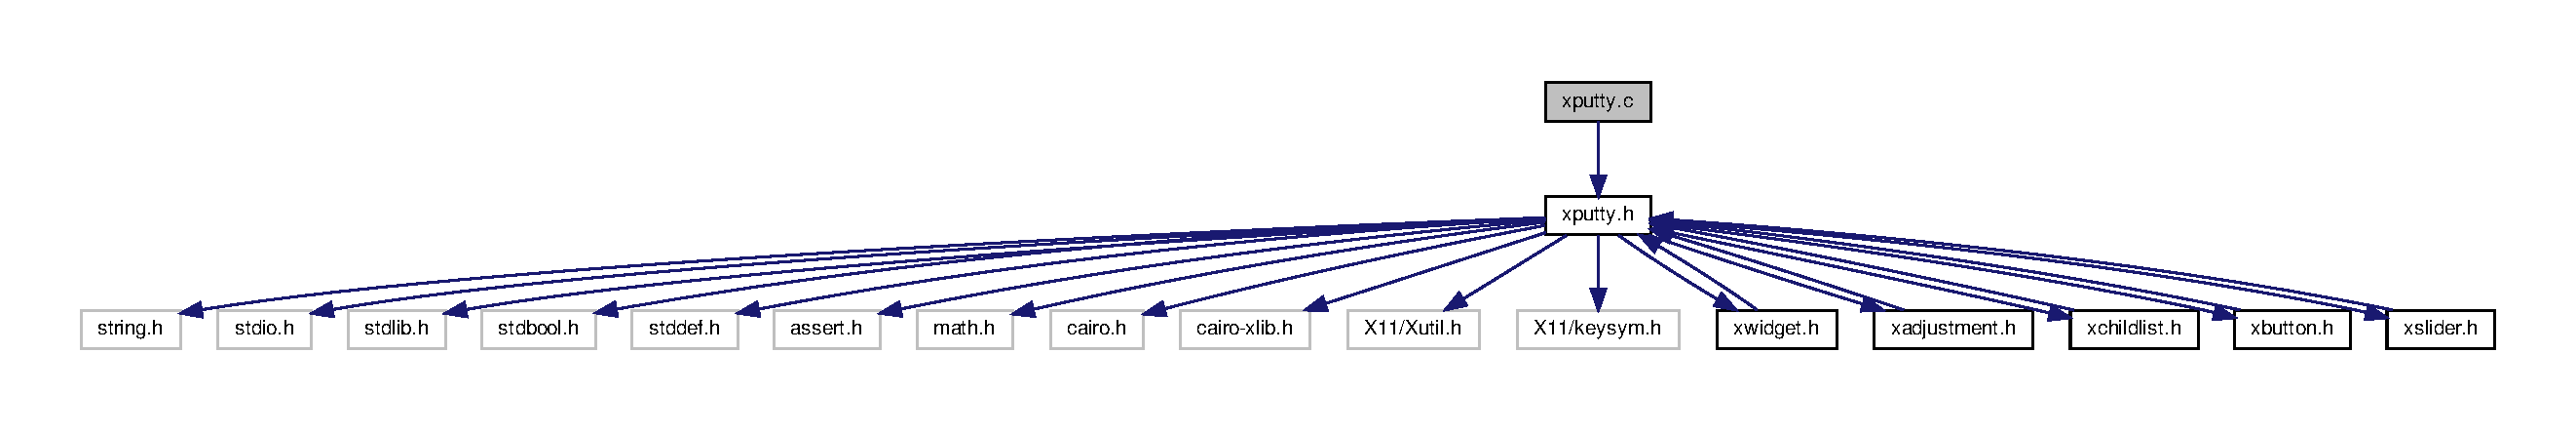
\includegraphics[width=350pt]{xputty_8c__incl}
\end{center}
\end{figure}
\subsection*{Functions}
\begin{DoxyCompactItemize}
\item 
void \hyperlink{xputty_8c_a484645d624d9e9eff0288f8d5583ff5e}{main\+\_\+init} (\hyperlink{structXputty}{Xputty} $\ast$main)
\begin{DoxyCompactList}\small\item\em main\+\_\+init -\/ init the \hyperlink{structXputty}{Xputty} struct \end{DoxyCompactList}\item 
void \hyperlink{xputty_8c_abb548ea64f852a7c94473a595e67d69f}{main\+\_\+run} (\hyperlink{structXputty}{Xputty} $\ast$main)
\begin{DoxyCompactList}\small\item\em main\+\_\+run -\/ the event loop \end{DoxyCompactList}\item 
void \hyperlink{xputty_8c_a0d4eda902b4de6f7a30e8d869f842fda}{main\+\_\+quit} (\hyperlink{structXputty}{Xputty} $\ast$main)
\begin{DoxyCompactList}\small\item\em main\+\_\+quit -\/ clean up afterr quiting the main loop \end{DoxyCompactList}\end{DoxyCompactItemize}


\subsection{Function Documentation}
\mbox{\Hypertarget{xputty_8c_a484645d624d9e9eff0288f8d5583ff5e}\label{xputty_8c_a484645d624d9e9eff0288f8d5583ff5e}} 
\index{xputty.\+c@{xputty.\+c}!main\+\_\+init@{main\+\_\+init}}
\index{main\+\_\+init@{main\+\_\+init}!xputty.\+c@{xputty.\+c}}
\subsubsection{\texorpdfstring{main\+\_\+init()}{main\_init()}}
{\footnotesize\ttfamily void main\+\_\+init (\begin{DoxyParamCaption}\item[{\hyperlink{structXputty}{Xputty} $\ast$}]{main }\end{DoxyParamCaption})}



main\+\_\+init -\/ init the \hyperlink{structXputty}{Xputty} struct 


\begin{DoxyParams}{Parameters}
{\em $\ast$main} & -\/ pointer to the main \hyperlink{structXputty}{Xputty} struct \\
\hline
\end{DoxyParams}
\begin{DoxyReturn}{Returns}
void 
\end{DoxyReturn}
\mbox{\Hypertarget{xputty_8c_a0d4eda902b4de6f7a30e8d869f842fda}\label{xputty_8c_a0d4eda902b4de6f7a30e8d869f842fda}} 
\index{xputty.\+c@{xputty.\+c}!main\+\_\+quit@{main\+\_\+quit}}
\index{main\+\_\+quit@{main\+\_\+quit}!xputty.\+c@{xputty.\+c}}
\subsubsection{\texorpdfstring{main\+\_\+quit()}{main\_quit()}}
{\footnotesize\ttfamily void main\+\_\+quit (\begin{DoxyParamCaption}\item[{\hyperlink{structXputty}{Xputty} $\ast$}]{main }\end{DoxyParamCaption})}



main\+\_\+quit -\/ clean up afterr quiting the main loop 


\begin{DoxyParams}{Parameters}
{\em $\ast$main} & -\/ pointer to the main \hyperlink{structXputty}{Xputty} struct \\
\hline
\end{DoxyParams}
\begin{DoxyReturn}{Returns}
void 
\end{DoxyReturn}
\mbox{\Hypertarget{xputty_8c_abb548ea64f852a7c94473a595e67d69f}\label{xputty_8c_abb548ea64f852a7c94473a595e67d69f}} 
\index{xputty.\+c@{xputty.\+c}!main\+\_\+run@{main\+\_\+run}}
\index{main\+\_\+run@{main\+\_\+run}!xputty.\+c@{xputty.\+c}}
\subsubsection{\texorpdfstring{main\+\_\+run()}{main\_run()}}
{\footnotesize\ttfamily void main\+\_\+run (\begin{DoxyParamCaption}\item[{\hyperlink{structXputty}{Xputty} $\ast$}]{main }\end{DoxyParamCaption})}



main\+\_\+run -\/ the event loop 

main\+\_\+run -\/ the main event loop


\begin{DoxyParams}{Parameters}
{\em $\ast$main} & -\/ pointer to the main \hyperlink{structXputty}{Xputty} struct \\
\hline
\end{DoxyParams}
\begin{DoxyReturn}{Returns}
void 
\end{DoxyReturn}

\hypertarget{xputty_8h}{}\section{xputty.\+h File Reference}
\label{xputty_8h}\index{xputty.\+h@{xputty.\+h}}
{\ttfamily \#include $<$string.\+h$>$}\newline
{\ttfamily \#include $<$stdio.\+h$>$}\newline
{\ttfamily \#include $<$stdlib.\+h$>$}\newline
{\ttfamily \#include $<$stdbool.\+h$>$}\newline
{\ttfamily \#include $<$stddef.\+h$>$}\newline
{\ttfamily \#include $<$assert.\+h$>$}\newline
{\ttfamily \#include $<$math.\+h$>$}\newline
{\ttfamily \#include $<$cairo.\+h$>$}\newline
{\ttfamily \#include $<$cairo-\/xlib.\+h$>$}\newline
{\ttfamily \#include $<$X11/\+Xutil.\+h$>$}\newline
{\ttfamily \#include $<$X11/keysym.\+h$>$}\newline
{\ttfamily \#include $<$X11/\+Xatom.\+h$>$}\newline
{\ttfamily \#include \char`\"{}xwidget.\+h\char`\"{}}\newline
{\ttfamily \#include \char`\"{}xadjustment.\+h\char`\"{}}\newline
{\ttfamily \#include \char`\"{}xchildlist.\+h\char`\"{}}\newline
{\ttfamily \#include \char`\"{}xcolor.\+h\char`\"{}}\newline
{\ttfamily \#include \char`\"{}xpngloader.\+h\char`\"{}}\newline
Include dependency graph for xputty.\+h\+:
\nopagebreak
\begin{figure}[H]
\begin{center}
\leavevmode
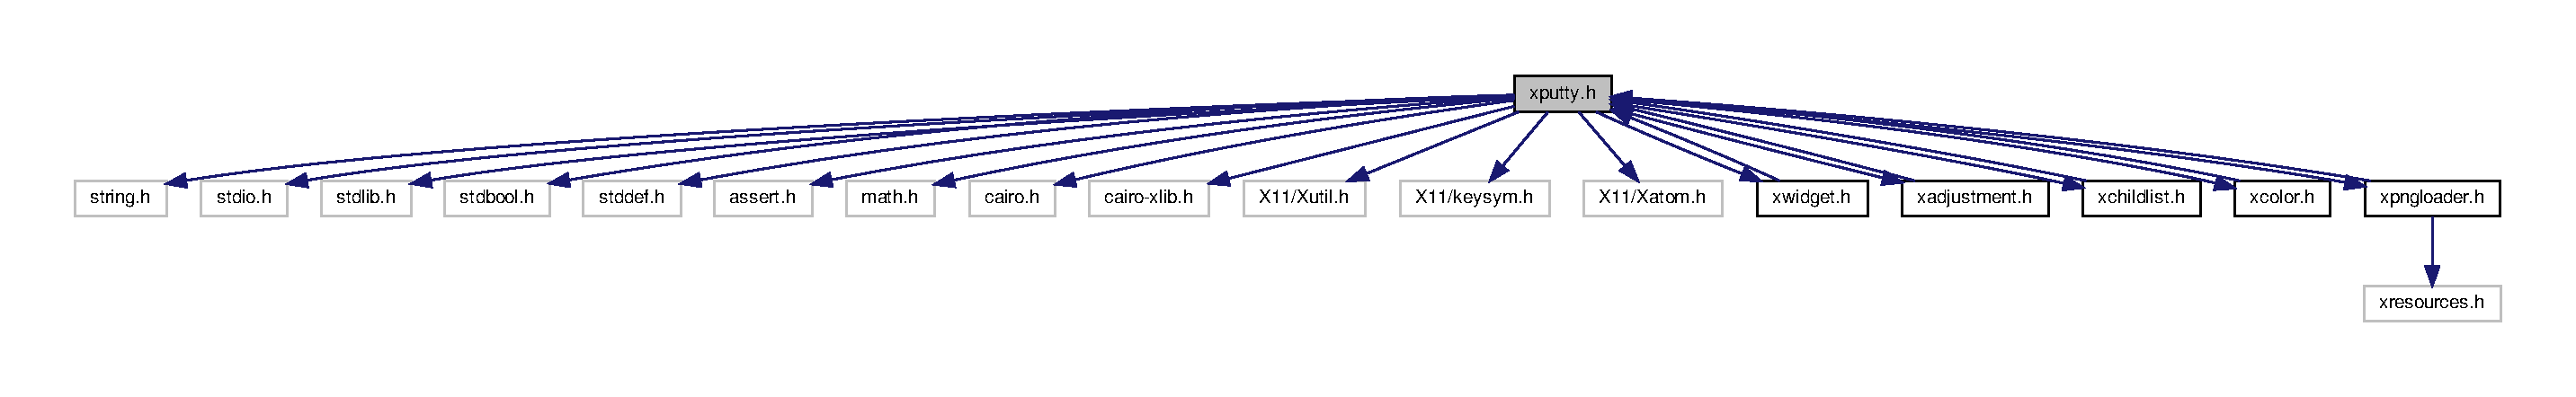
\includegraphics[width=350pt]{xputty_8h__incl}
\end{center}
\end{figure}
This graph shows which files directly or indirectly include this file\+:
\nopagebreak
\begin{figure}[H]
\begin{center}
\leavevmode
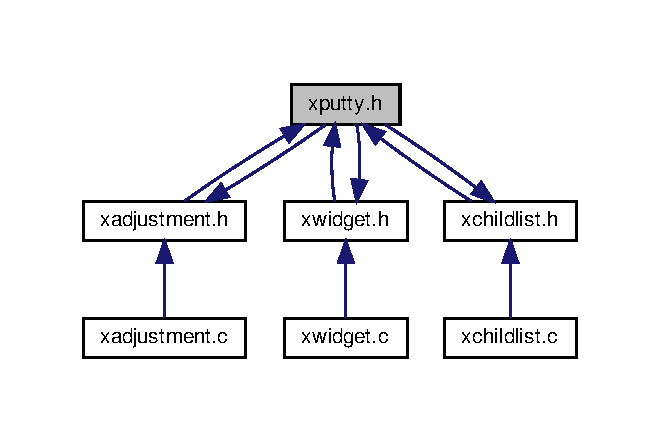
\includegraphics[width=350pt]{xputty_8h__dep__incl}
\end{center}
\end{figure}
\subsection*{Data Structures}
\begin{DoxyCompactItemize}
\item 
struct \hyperlink{structXputty}{Xputty}
\begin{DoxyCompactList}\small\item\em \hyperlink{structXputty}{Xputty} -\/ the main struct. It should be declared before any other call to a \hyperlink{structXputty}{Xputty} function. \end{DoxyCompactList}\end{DoxyCompactItemize}
\subsection*{Macros}
\begin{DoxyCompactItemize}
\item 
\#define \hyperlink{xputty_8h_accb46852f2244dde7d0e696c1380263e}{X\+P\+U\+T\+T\+Y1\+\_\+\+H\+\_\+}
\item 
\#define \hyperlink{xputty_8h_ad72dbcf6d0153db1b8d8a58001feed83}{D\+E\+B\+UG}~0
\item 
\#define \hyperlink{xputty_8h_a8de3ed741dadc9c979a4ff17c0a9116e}{N\+D\+E\+B\+UG}
\item 
\#define \hyperlink{xputty_8h_ac9e7326b4569847122754061b96c42d0}{debug\+\_\+print}(...)~((void)((\hyperlink{xputty_8h_ad72dbcf6d0153db1b8d8a58001feed83}{D\+E\+B\+UG}) ? fprintf(stderr, \+\_\+\+\_\+\+V\+A\+\_\+\+A\+R\+G\+S\+\_\+\+\_\+) \+: 0))
\begin{DoxyCompactList}\small\item\em debug\+\_\+print -\/ print out state messages when compiled with the -\/\+D\+D\+E\+B\+UG flag \end{DoxyCompactList}\item 
\#define \hyperlink{xputty_8h_abb702d8b501669a23aa0ab3b281b9384}{min}(x,  y)~((x) $<$ (y) ? (x) \+: (y))
\begin{DoxyCompactList}\small\item\em min -\/ set a maximal value (x) as return value \end{DoxyCompactList}\item 
\#define \hyperlink{xputty_8h_ac39d9cef6a5e030ba8d9e11121054268}{max}(x,  y)~((x) $<$ (y) ? (y) \+: (x))
\begin{DoxyCompactList}\small\item\em max -\/ set a minimal value (x) as return value \end{DoxyCompactList}\item 
\#define \hyperlink{xputty_8h_a4b4e4f21ac252ef0b97fe32f026bd284}{I\+S\+\_\+\+U\+T\+F8}(c)~(((c)\&0xc0)==0xc0)
\begin{DoxyCompactList}\small\item\em I\+S\+\_\+\+U\+T\+F8 -\/ check if a char contain U\+TF 8 formated signs. \end{DoxyCompactList}\end{DoxyCompactItemize}
\subsection*{Typedefs}
\begin{DoxyCompactItemize}
\item 
typedef struct \hyperlink{structChildlist__t}{Childlist\+\_\+t} \hyperlink{xputty_8h_a972f6c1b2363cd41766d32dc7d3a93d0}{Childlist\+\_\+t}
\begin{DoxyCompactList}\small\item\em \hyperlink{structChildlist__t}{Childlist\+\_\+t} -\/ maintain a \hyperlink{structWidget__t}{Widget\+\_\+t} list of childs for a \hyperlink{structWidget__t}{Widget\+\_\+t}. \end{DoxyCompactList}\item 
typedef struct \hyperlink{structAdjustment__t}{Adjustment\+\_\+t} \hyperlink{xputty_8h_a68965e5ced4b615cf52922868c4b159c}{Adjustment\+\_\+t}
\begin{DoxyCompactList}\small\item\em \hyperlink{structAdjustment__t}{Adjustment\+\_\+t} -\/ \hyperlink{structAdjustment__t}{Adjustment\+\_\+t} for a \hyperlink{structWidget__t}{Widget\+\_\+t}. \end{DoxyCompactList}\item 
typedef struct \hyperlink{structWidget__t}{Widget\+\_\+t} \hyperlink{xputty_8h_a6b3e8ecb43e49de5de9dc7ab79404014}{Widget\+\_\+t}
\begin{DoxyCompactList}\small\item\em \hyperlink{structWidget__t}{Widget\+\_\+t} -\/ the \hyperlink{structWidget__t}{Widget\+\_\+t} base struct. \end{DoxyCompactList}\item 
typedef struct \hyperlink{structXColor__t}{X\+Color\+\_\+t} \hyperlink{xputty_8h_a8fd8b2af101a65738477a274b3894153}{X\+Color\+\_\+t}
\begin{DoxyCompactList}\small\item\em \hyperlink{structXColor__t}{X\+Color\+\_\+t} -\/ the \hyperlink{structWidget__t}{Widget\+\_\+t} Color struct. \end{DoxyCompactList}\item 
typedef struct \hyperlink{structXputty}{Xputty} \hyperlink{xputty_8h_a640738d2c0bf1af308958da6468c829f}{Xputty}
\begin{DoxyCompactList}\small\item\em \hyperlink{structXputty}{Xputty} -\/ the main struct.\+It should be declared before any other call to a \hyperlink{structXputty}{Xputty} function. \end{DoxyCompactList}\end{DoxyCompactItemize}
\subsection*{Functions}
\begin{DoxyCompactItemize}
\item 
void \hyperlink{xputty_8h_a484645d624d9e9eff0288f8d5583ff5e}{main\+\_\+init} (\hyperlink{structXputty}{Xputty} $\ast$main)
\begin{DoxyCompactList}\small\item\em main\+\_\+init -\/ open the Display and init the main-\/$>$childlist. Also it set the bool run to true. This one will be used to terminate the main event loop. \hyperlink{xputty_8h_a484645d624d9e9eff0288f8d5583ff5e}{main\+\_\+init()} should be called directly after declaration of \hyperlink{structXputty}{Xputty}. Any \hyperlink{structWidget__t}{Widget\+\_\+t} which would be created afterwards will be added to the list. This list is used to check if a \hyperlink{structWidget__t}{Widget\+\_\+t} is valid. When a \hyperlink{structWidget__t}{Widget\+\_\+t} call \hyperlink{xwidget_8c_a1e367c7f3e7dcd71fbbb6125fc1b227a}{quit\+\_\+widget()} it will be removed from the list. On \hyperlink{xputty_8h_a0d4eda902b4de6f7a30e8d869f842fda}{main\+\_\+quit()} any remaining \hyperlink{structWidget__t}{Widget\+\_\+t} from this list will be destroyed, to ensure that we leave the memory clean. This list is also used to check which Window receive a X\+Event. \end{DoxyCompactList}\item 
void \hyperlink{xputty_8h_abb548ea64f852a7c94473a595e67d69f}{main\+\_\+run} (\hyperlink{structXputty}{Xputty} $\ast$main)
\begin{DoxyCompactList}\small\item\em main\+\_\+run -\/ the main event loop. It should be start after your \hyperlink{structWidget__t}{Widget\+\_\+t}\textquotesingle{}s been created. You could create and destroy additional \hyperlink{structWidget__t}{Widget\+\_\+t}\textquotesingle{}s at any time later during run. \end{DoxyCompactList}\item 
void \hyperlink{xputty_8h_ad265582bb835c54e689b2c354e8dd865}{run\+\_\+embedded} (\hyperlink{structXputty}{Xputty} $\ast$main)
\begin{DoxyCompactList}\small\item\em run\+\_\+embedded -\/ the main event loop to run embedded UI\textquotesingle{}s. It should be start after your \hyperlink{structWidget__t}{Widget\+\_\+t}\textquotesingle{}s been created. You could create and destroy additional \hyperlink{structWidget__t}{Widget\+\_\+t}\textquotesingle{}s at any time later during run. \end{DoxyCompactList}\item 
void \hyperlink{xputty_8h_a0d4eda902b4de6f7a30e8d869f842fda}{main\+\_\+quit} (\hyperlink{structXputty}{Xputty} $\ast$main)
\begin{DoxyCompactList}\small\item\em main\+\_\+quit -\/ destroy all remaining \hyperlink{structWidget__t}{Widget\+\_\+t}\textquotesingle{}s from the main-\/$>$childlist. Free all resources which may be allocated between init and quit. It should be called after \hyperlink{xputty_8h_abb548ea64f852a7c94473a595e67d69f}{main\+\_\+run()}; \end{DoxyCompactList}\end{DoxyCompactItemize}


\subsection{Macro Definition Documentation}
\mbox{\Hypertarget{xputty_8h_ad72dbcf6d0153db1b8d8a58001feed83}\label{xputty_8h_ad72dbcf6d0153db1b8d8a58001feed83}} 
\index{xputty.\+h@{xputty.\+h}!D\+E\+B\+UG@{D\+E\+B\+UG}}
\index{D\+E\+B\+UG@{D\+E\+B\+UG}!xputty.\+h@{xputty.\+h}}
\subsubsection{\texorpdfstring{D\+E\+B\+UG}{DEBUG}}
{\footnotesize\ttfamily \#define D\+E\+B\+UG~0}

\mbox{\Hypertarget{xputty_8h_ac9e7326b4569847122754061b96c42d0}\label{xputty_8h_ac9e7326b4569847122754061b96c42d0}} 
\index{xputty.\+h@{xputty.\+h}!debug\+\_\+print@{debug\+\_\+print}}
\index{debug\+\_\+print@{debug\+\_\+print}!xputty.\+h@{xputty.\+h}}
\subsubsection{\texorpdfstring{debug\+\_\+print}{debug\_print}}
{\footnotesize\ttfamily \#define debug\+\_\+print(\begin{DoxyParamCaption}\item[{}]{... }\end{DoxyParamCaption})~((void)((\hyperlink{xputty_8h_ad72dbcf6d0153db1b8d8a58001feed83}{D\+E\+B\+UG}) ? fprintf(stderr, \+\_\+\+\_\+\+V\+A\+\_\+\+A\+R\+G\+S\+\_\+\+\_\+) \+: 0))}



debug\+\_\+print -\/ print out state messages when compiled with the -\/\+D\+D\+E\+B\+UG flag 

\mbox{\Hypertarget{xputty_8h_a4b4e4f21ac252ef0b97fe32f026bd284}\label{xputty_8h_a4b4e4f21ac252ef0b97fe32f026bd284}} 
\index{xputty.\+h@{xputty.\+h}!I\+S\+\_\+\+U\+T\+F8@{I\+S\+\_\+\+U\+T\+F8}}
\index{I\+S\+\_\+\+U\+T\+F8@{I\+S\+\_\+\+U\+T\+F8}!xputty.\+h@{xputty.\+h}}
\subsubsection{\texorpdfstring{I\+S\+\_\+\+U\+T\+F8}{IS\_UTF8}}
{\footnotesize\ttfamily \#define I\+S\+\_\+\+U\+T\+F8(\begin{DoxyParamCaption}\item[{}]{c }\end{DoxyParamCaption})~(((c)\&0xc0)==0xc0)}



I\+S\+\_\+\+U\+T\+F8 -\/ check if a char contain U\+TF 8 formated signs. 

\mbox{\Hypertarget{xputty_8h_ac39d9cef6a5e030ba8d9e11121054268}\label{xputty_8h_ac39d9cef6a5e030ba8d9e11121054268}} 
\index{xputty.\+h@{xputty.\+h}!max@{max}}
\index{max@{max}!xputty.\+h@{xputty.\+h}}
\subsubsection{\texorpdfstring{max}{max}}
{\footnotesize\ttfamily \#define max(\begin{DoxyParamCaption}\item[{}]{x,  }\item[{}]{y }\end{DoxyParamCaption})~((x) $<$ (y) ? (y) \+: (x))}



max -\/ set a minimal value (x) as return value 

\mbox{\Hypertarget{xputty_8h_abb702d8b501669a23aa0ab3b281b9384}\label{xputty_8h_abb702d8b501669a23aa0ab3b281b9384}} 
\index{xputty.\+h@{xputty.\+h}!min@{min}}
\index{min@{min}!xputty.\+h@{xputty.\+h}}
\subsubsection{\texorpdfstring{min}{min}}
{\footnotesize\ttfamily \#define min(\begin{DoxyParamCaption}\item[{}]{x,  }\item[{}]{y }\end{DoxyParamCaption})~((x) $<$ (y) ? (x) \+: (y))}



min -\/ set a maximal value (x) as return value 

\mbox{\Hypertarget{xputty_8h_a8de3ed741dadc9c979a4ff17c0a9116e}\label{xputty_8h_a8de3ed741dadc9c979a4ff17c0a9116e}} 
\index{xputty.\+h@{xputty.\+h}!N\+D\+E\+B\+UG@{N\+D\+E\+B\+UG}}
\index{N\+D\+E\+B\+UG@{N\+D\+E\+B\+UG}!xputty.\+h@{xputty.\+h}}
\subsubsection{\texorpdfstring{N\+D\+E\+B\+UG}{NDEBUG}}
{\footnotesize\ttfamily \#define N\+D\+E\+B\+UG}

\mbox{\Hypertarget{xputty_8h_accb46852f2244dde7d0e696c1380263e}\label{xputty_8h_accb46852f2244dde7d0e696c1380263e}} 
\index{xputty.\+h@{xputty.\+h}!X\+P\+U\+T\+T\+Y1\+\_\+\+H\+\_\+@{X\+P\+U\+T\+T\+Y1\+\_\+\+H\+\_\+}}
\index{X\+P\+U\+T\+T\+Y1\+\_\+\+H\+\_\+@{X\+P\+U\+T\+T\+Y1\+\_\+\+H\+\_\+}!xputty.\+h@{xputty.\+h}}
\subsubsection{\texorpdfstring{X\+P\+U\+T\+T\+Y1\+\_\+\+H\+\_\+}{XPUTTY1\_H\_}}
{\footnotesize\ttfamily \#define X\+P\+U\+T\+T\+Y1\+\_\+\+H\+\_\+}



\subsection{Typedef Documentation}
\mbox{\Hypertarget{xputty_8h_a68965e5ced4b615cf52922868c4b159c}\label{xputty_8h_a68965e5ced4b615cf52922868c4b159c}} 
\index{xputty.\+h@{xputty.\+h}!Adjustment\+\_\+t@{Adjustment\+\_\+t}}
\index{Adjustment\+\_\+t@{Adjustment\+\_\+t}!xputty.\+h@{xputty.\+h}}
\subsubsection{\texorpdfstring{Adjustment\+\_\+t}{Adjustment\_t}}
{\footnotesize\ttfamily typedef struct \hyperlink{structAdjustment__t}{Adjustment\+\_\+t} \hyperlink{structAdjustment__t}{Adjustment\+\_\+t}}



\hyperlink{structAdjustment__t}{Adjustment\+\_\+t} -\/ \hyperlink{structAdjustment__t}{Adjustment\+\_\+t} for a \hyperlink{structWidget__t}{Widget\+\_\+t}. 

\mbox{\Hypertarget{xputty_8h_a972f6c1b2363cd41766d32dc7d3a93d0}\label{xputty_8h_a972f6c1b2363cd41766d32dc7d3a93d0}} 
\index{xputty.\+h@{xputty.\+h}!Childlist\+\_\+t@{Childlist\+\_\+t}}
\index{Childlist\+\_\+t@{Childlist\+\_\+t}!xputty.\+h@{xputty.\+h}}
\subsubsection{\texorpdfstring{Childlist\+\_\+t}{Childlist\_t}}
{\footnotesize\ttfamily typedef struct \hyperlink{structChildlist__t}{Childlist\+\_\+t} \hyperlink{structChildlist__t}{Childlist\+\_\+t}}



\hyperlink{structChildlist__t}{Childlist\+\_\+t} -\/ maintain a \hyperlink{structWidget__t}{Widget\+\_\+t} list of childs for a \hyperlink{structWidget__t}{Widget\+\_\+t}. 

\mbox{\Hypertarget{xputty_8h_a6b3e8ecb43e49de5de9dc7ab79404014}\label{xputty_8h_a6b3e8ecb43e49de5de9dc7ab79404014}} 
\index{xputty.\+h@{xputty.\+h}!Widget\+\_\+t@{Widget\+\_\+t}}
\index{Widget\+\_\+t@{Widget\+\_\+t}!xputty.\+h@{xputty.\+h}}
\subsubsection{\texorpdfstring{Widget\+\_\+t}{Widget\_t}}
{\footnotesize\ttfamily typedef struct \hyperlink{structWidget__t}{Widget\+\_\+t} \hyperlink{structWidget__t}{Widget\+\_\+t}}



\hyperlink{structWidget__t}{Widget\+\_\+t} -\/ the \hyperlink{structWidget__t}{Widget\+\_\+t} base struct. 

\mbox{\Hypertarget{xputty_8h_a8fd8b2af101a65738477a274b3894153}\label{xputty_8h_a8fd8b2af101a65738477a274b3894153}} 
\index{xputty.\+h@{xputty.\+h}!X\+Color\+\_\+t@{X\+Color\+\_\+t}}
\index{X\+Color\+\_\+t@{X\+Color\+\_\+t}!xputty.\+h@{xputty.\+h}}
\subsubsection{\texorpdfstring{X\+Color\+\_\+t}{XColor\_t}}
{\footnotesize\ttfamily typedef struct \hyperlink{structXColor__t}{X\+Color\+\_\+t} \hyperlink{structXColor__t}{X\+Color\+\_\+t}}



\hyperlink{structXColor__t}{X\+Color\+\_\+t} -\/ the \hyperlink{structWidget__t}{Widget\+\_\+t} Color struct. 

\mbox{\Hypertarget{xputty_8h_a640738d2c0bf1af308958da6468c829f}\label{xputty_8h_a640738d2c0bf1af308958da6468c829f}} 
\index{xputty.\+h@{xputty.\+h}!Xputty@{Xputty}}
\index{Xputty@{Xputty}!xputty.\+h@{xputty.\+h}}
\subsubsection{\texorpdfstring{Xputty}{Xputty}}
{\footnotesize\ttfamily typedef struct \hyperlink{structXputty}{Xputty} \hyperlink{structXputty}{Xputty}}



\hyperlink{structXputty}{Xputty} -\/ the main struct.\+It should be declared before any other call to a \hyperlink{structXputty}{Xputty} function. 



\subsection{Function Documentation}
\mbox{\Hypertarget{xputty_8h_a484645d624d9e9eff0288f8d5583ff5e}\label{xputty_8h_a484645d624d9e9eff0288f8d5583ff5e}} 
\index{xputty.\+h@{xputty.\+h}!main\+\_\+init@{main\+\_\+init}}
\index{main\+\_\+init@{main\+\_\+init}!xputty.\+h@{xputty.\+h}}
\subsubsection{\texorpdfstring{main\+\_\+init()}{main\_init()}}
{\footnotesize\ttfamily void main\+\_\+init (\begin{DoxyParamCaption}\item[{\hyperlink{structXputty}{Xputty} $\ast$}]{main }\end{DoxyParamCaption})}



main\+\_\+init -\/ open the Display and init the main-\/$>$childlist. Also it set the bool run to true. This one will be used to terminate the main event loop. \hyperlink{xputty_8h_a484645d624d9e9eff0288f8d5583ff5e}{main\+\_\+init()} should be called directly after declaration of \hyperlink{structXputty}{Xputty}. Any \hyperlink{structWidget__t}{Widget\+\_\+t} which would be created afterwards will be added to the list. This list is used to check if a \hyperlink{structWidget__t}{Widget\+\_\+t} is valid. When a \hyperlink{structWidget__t}{Widget\+\_\+t} call \hyperlink{xwidget_8c_a1e367c7f3e7dcd71fbbb6125fc1b227a}{quit\+\_\+widget()} it will be removed from the list. On \hyperlink{xputty_8h_a0d4eda902b4de6f7a30e8d869f842fda}{main\+\_\+quit()} any remaining \hyperlink{structWidget__t}{Widget\+\_\+t} from this list will be destroyed, to ensure that we leave the memory clean. This list is also used to check which Window receive a X\+Event. 


\begin{DoxyParams}{Parameters}
{\em $\ast$main} & -\/ pointer to the main \hyperlink{structXputty}{Xputty} struct \\
\hline
\end{DoxyParams}
\begin{DoxyReturn}{Returns}
void 
\end{DoxyReturn}
\mbox{\Hypertarget{xputty_8h_a0d4eda902b4de6f7a30e8d869f842fda}\label{xputty_8h_a0d4eda902b4de6f7a30e8d869f842fda}} 
\index{xputty.\+h@{xputty.\+h}!main\+\_\+quit@{main\+\_\+quit}}
\index{main\+\_\+quit@{main\+\_\+quit}!xputty.\+h@{xputty.\+h}}
\subsubsection{\texorpdfstring{main\+\_\+quit()}{main\_quit()}}
{\footnotesize\ttfamily void main\+\_\+quit (\begin{DoxyParamCaption}\item[{\hyperlink{structXputty}{Xputty} $\ast$}]{main }\end{DoxyParamCaption})}



main\+\_\+quit -\/ destroy all remaining \hyperlink{structWidget__t}{Widget\+\_\+t}\textquotesingle{}s from the main-\/$>$childlist. Free all resources which may be allocated between init and quit. It should be called after \hyperlink{xputty_8h_abb548ea64f852a7c94473a595e67d69f}{main\+\_\+run()}; 


\begin{DoxyParams}{Parameters}
{\em $\ast$main} & -\/ pointer to the main \hyperlink{structXputty}{Xputty} struct \\
\hline
\end{DoxyParams}
\begin{DoxyReturn}{Returns}
void 
\end{DoxyReturn}
\mbox{\Hypertarget{xputty_8h_abb548ea64f852a7c94473a595e67d69f}\label{xputty_8h_abb548ea64f852a7c94473a595e67d69f}} 
\index{xputty.\+h@{xputty.\+h}!main\+\_\+run@{main\+\_\+run}}
\index{main\+\_\+run@{main\+\_\+run}!xputty.\+h@{xputty.\+h}}
\subsubsection{\texorpdfstring{main\+\_\+run()}{main\_run()}}
{\footnotesize\ttfamily void main\+\_\+run (\begin{DoxyParamCaption}\item[{\hyperlink{structXputty}{Xputty} $\ast$}]{main }\end{DoxyParamCaption})}



main\+\_\+run -\/ the main event loop. It should be start after your \hyperlink{structWidget__t}{Widget\+\_\+t}\textquotesingle{}s been created. You could create and destroy additional \hyperlink{structWidget__t}{Widget\+\_\+t}\textquotesingle{}s at any time later during run. 


\begin{DoxyParams}{Parameters}
{\em $\ast$main} & -\/ pointer to the main \hyperlink{structXputty}{Xputty} struct \\
\hline
\end{DoxyParams}
\begin{DoxyReturn}{Returns}
void 
\end{DoxyReturn}
\mbox{\Hypertarget{xputty_8h_ad265582bb835c54e689b2c354e8dd865}\label{xputty_8h_ad265582bb835c54e689b2c354e8dd865}} 
\index{xputty.\+h@{xputty.\+h}!run\+\_\+embedded@{run\+\_\+embedded}}
\index{run\+\_\+embedded@{run\+\_\+embedded}!xputty.\+h@{xputty.\+h}}
\subsubsection{\texorpdfstring{run\+\_\+embedded()}{run\_embedded()}}
{\footnotesize\ttfamily void run\+\_\+embedded (\begin{DoxyParamCaption}\item[{\hyperlink{structXputty}{Xputty} $\ast$}]{main }\end{DoxyParamCaption})}



run\+\_\+embedded -\/ the main event loop to run embedded UI\textquotesingle{}s. It should be start after your \hyperlink{structWidget__t}{Widget\+\_\+t}\textquotesingle{}s been created. You could create and destroy additional \hyperlink{structWidget__t}{Widget\+\_\+t}\textquotesingle{}s at any time later during run. 


\begin{DoxyParams}{Parameters}
{\em $\ast$main} & -\/ pointer to the main \hyperlink{structXputty}{Xputty} struct \\
\hline
\end{DoxyParams}
\begin{DoxyReturn}{Returns}
void 
\end{DoxyReturn}

\hypertarget{xslider_8c}{}\section{xslider.\+c File Reference}
\label{xslider_8c}\index{xslider.\+c@{xslider.\+c}}
{\ttfamily \#include \char`\"{}xslider.\+h\char`\"{}}\newline
{\ttfamily \#include \char`\"{}xslider\+\_\+private.\+h\char`\"{}}\newline
Include dependency graph for xslider.\+c\+:
\nopagebreak
\begin{figure}[H]
\begin{center}
\leavevmode
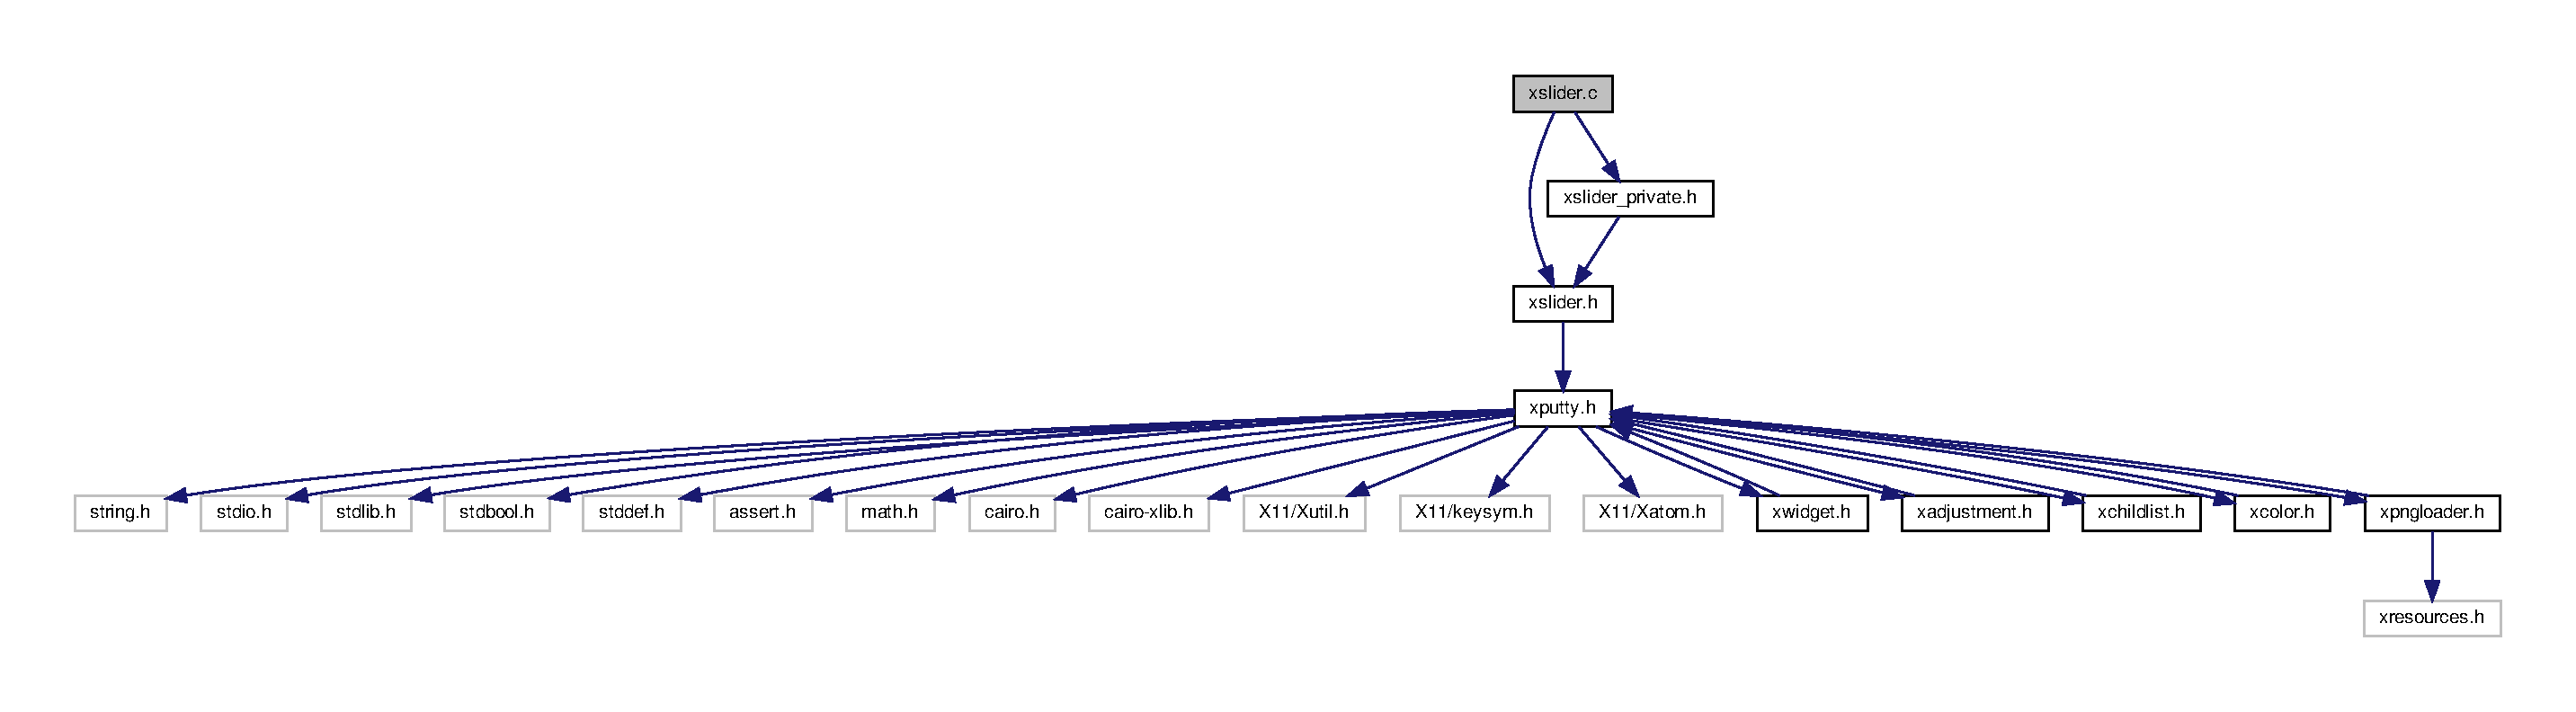
\includegraphics[width=350pt]{xslider_8c__incl}
\end{center}
\end{figure}
\subsection*{Functions}
\begin{DoxyCompactItemize}
\item 
\hyperlink{structWidget__t}{Widget\+\_\+t} $\ast$ \hyperlink{xslider_8c_a80c7eeb4a1b25c6fcb855d407d959b48}{add\+\_\+vslider} (\hyperlink{structWidget__t}{Widget\+\_\+t} $\ast$parent, const char $\ast$label, int x, int y, int width, int height)
\begin{DoxyCompactList}\small\item\em add\+\_\+vslider -\/ add a vertical slider to a \hyperlink{structWidget__t}{Widget\+\_\+t} connect to func.\+adj\+\_\+callback to implement your actions use set\+\_\+adjustment(w-\/$>$adj\+\_\+y, . . ) to set the range you need \end{DoxyCompactList}\item 
\hyperlink{structWidget__t}{Widget\+\_\+t} $\ast$ \hyperlink{xslider_8c_a508d0eea38b9c3a8b1e769b0e502c5bc}{add\+\_\+hslider} (\hyperlink{structWidget__t}{Widget\+\_\+t} $\ast$parent, const char $\ast$label, int x, int y, int width, int height)
\begin{DoxyCompactList}\small\item\em add\+\_\+hslider -\/ add a horizontal slider to a \hyperlink{structWidget__t}{Widget\+\_\+t} connect to func.\+adj\+\_\+callback to implement your actions use set\+\_\+adjustment(w-\/$>$adj\+\_\+x, . . ) to set the range you need \end{DoxyCompactList}\end{DoxyCompactItemize}


\subsection{Function Documentation}
\mbox{\Hypertarget{xslider_8c_a508d0eea38b9c3a8b1e769b0e502c5bc}\label{xslider_8c_a508d0eea38b9c3a8b1e769b0e502c5bc}} 
\index{xslider.\+c@{xslider.\+c}!add\+\_\+hslider@{add\+\_\+hslider}}
\index{add\+\_\+hslider@{add\+\_\+hslider}!xslider.\+c@{xslider.\+c}}
\subsubsection{\texorpdfstring{add\+\_\+hslider()}{add\_hslider()}}
{\footnotesize\ttfamily \hyperlink{structWidget__t}{Widget\+\_\+t}$\ast$ add\+\_\+hslider (\begin{DoxyParamCaption}\item[{\hyperlink{structWidget__t}{Widget\+\_\+t} $\ast$}]{parent,  }\item[{const char $\ast$}]{label,  }\item[{int}]{x,  }\item[{int}]{y,  }\item[{int}]{width,  }\item[{int}]{height }\end{DoxyParamCaption})}



add\+\_\+hslider -\/ add a horizontal slider to a \hyperlink{structWidget__t}{Widget\+\_\+t} connect to func.\+adj\+\_\+callback to implement your actions use set\+\_\+adjustment(w-\/$>$adj\+\_\+x, . . ) to set the range you need 


\begin{DoxyParams}{Parameters}
{\em $\ast$parent} & -\/ pointer to the \hyperlink{structWidget__t}{Widget\+\_\+t} request the button \\
\hline
{\em $\ast$label} & -\/ Label to show on the button \\
\hline
{\em x,y,width,height} & -\/ the position/geometry to create the button \\
\hline
\end{DoxyParams}
\begin{DoxyReturn}{Returns}
Widget\+\_\+t$\ast$ -\/ pointer to the \hyperlink{structWidget__t}{Widget\+\_\+t} button struct 
\end{DoxyReturn}
\mbox{\Hypertarget{xslider_8c_a80c7eeb4a1b25c6fcb855d407d959b48}\label{xslider_8c_a80c7eeb4a1b25c6fcb855d407d959b48}} 
\index{xslider.\+c@{xslider.\+c}!add\+\_\+vslider@{add\+\_\+vslider}}
\index{add\+\_\+vslider@{add\+\_\+vslider}!xslider.\+c@{xslider.\+c}}
\subsubsection{\texorpdfstring{add\+\_\+vslider()}{add\_vslider()}}
{\footnotesize\ttfamily \hyperlink{structWidget__t}{Widget\+\_\+t}$\ast$ add\+\_\+vslider (\begin{DoxyParamCaption}\item[{\hyperlink{structWidget__t}{Widget\+\_\+t} $\ast$}]{parent,  }\item[{const char $\ast$}]{label,  }\item[{int}]{x,  }\item[{int}]{y,  }\item[{int}]{width,  }\item[{int}]{height }\end{DoxyParamCaption})}



add\+\_\+vslider -\/ add a vertical slider to a \hyperlink{structWidget__t}{Widget\+\_\+t} connect to func.\+adj\+\_\+callback to implement your actions use set\+\_\+adjustment(w-\/$>$adj\+\_\+y, . . ) to set the range you need 


\begin{DoxyParams}{Parameters}
{\em $\ast$parent} & -\/ pointer to the \hyperlink{structWidget__t}{Widget\+\_\+t} request the button \\
\hline
{\em $\ast$label} & -\/ Label to show on the button \\
\hline
{\em x,y,width,height} & -\/ the position/geometry to create the button \\
\hline
\end{DoxyParams}
\begin{DoxyReturn}{Returns}
Widget\+\_\+t$\ast$ -\/ pointer to the \hyperlink{structWidget__t}{Widget\+\_\+t} button struct 
\end{DoxyReturn}

\hypertarget{xslider_8h}{}\section{xslider.\+h File Reference}
\label{xslider_8h}\index{xslider.\+h@{xslider.\+h}}
{\ttfamily \#include \char`\"{}xputty.\+h\char`\"{}}\newline
Include dependency graph for xslider.\+h\+:
\nopagebreak
\begin{figure}[H]
\begin{center}
\leavevmode
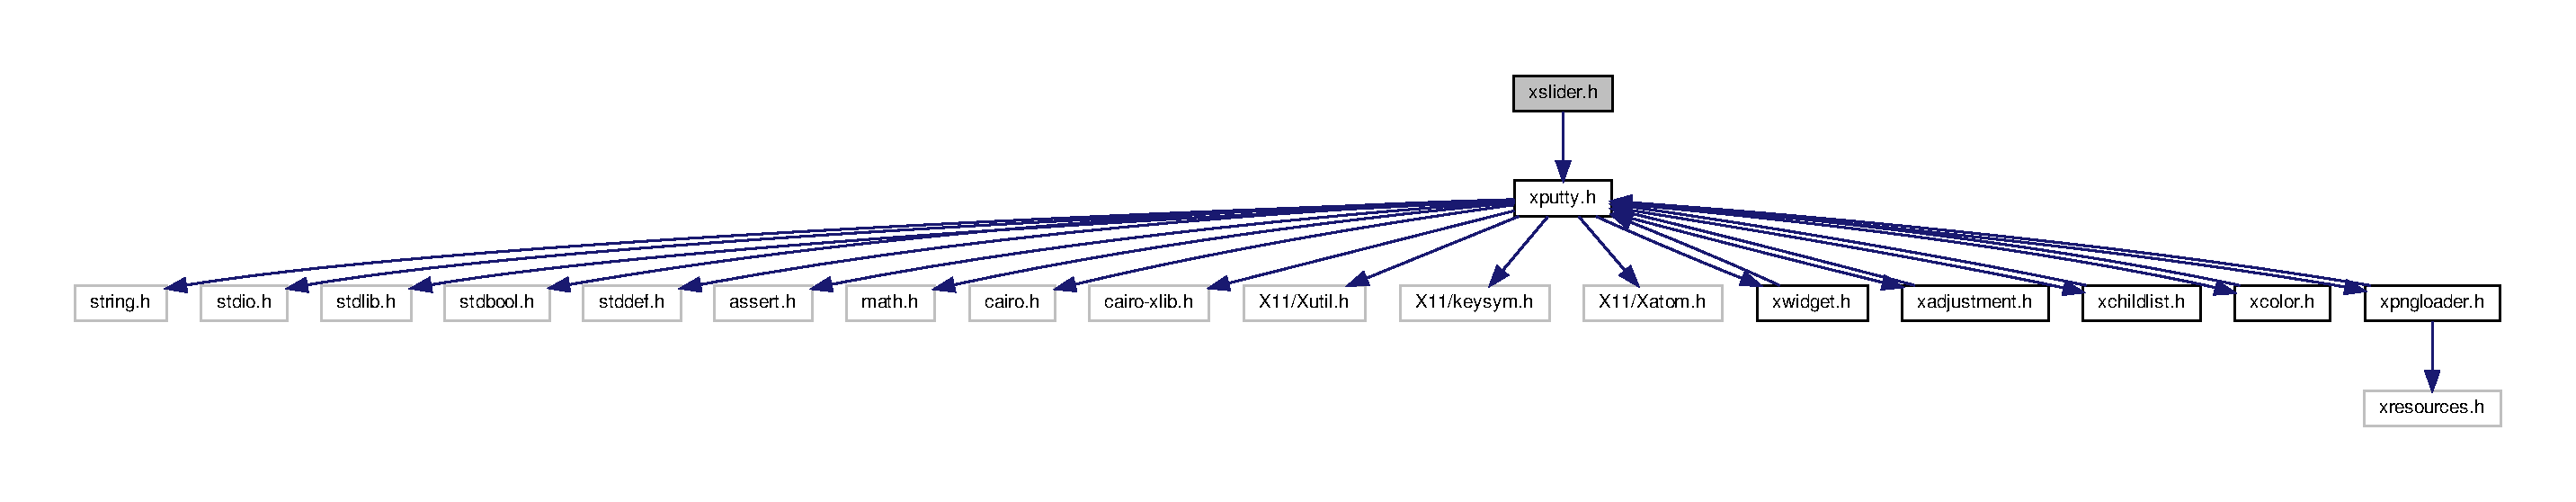
\includegraphics[width=350pt]{xslider_8h__incl}
\end{center}
\end{figure}
This graph shows which files directly or indirectly include this file\+:
\nopagebreak
\begin{figure}[H]
\begin{center}
\leavevmode
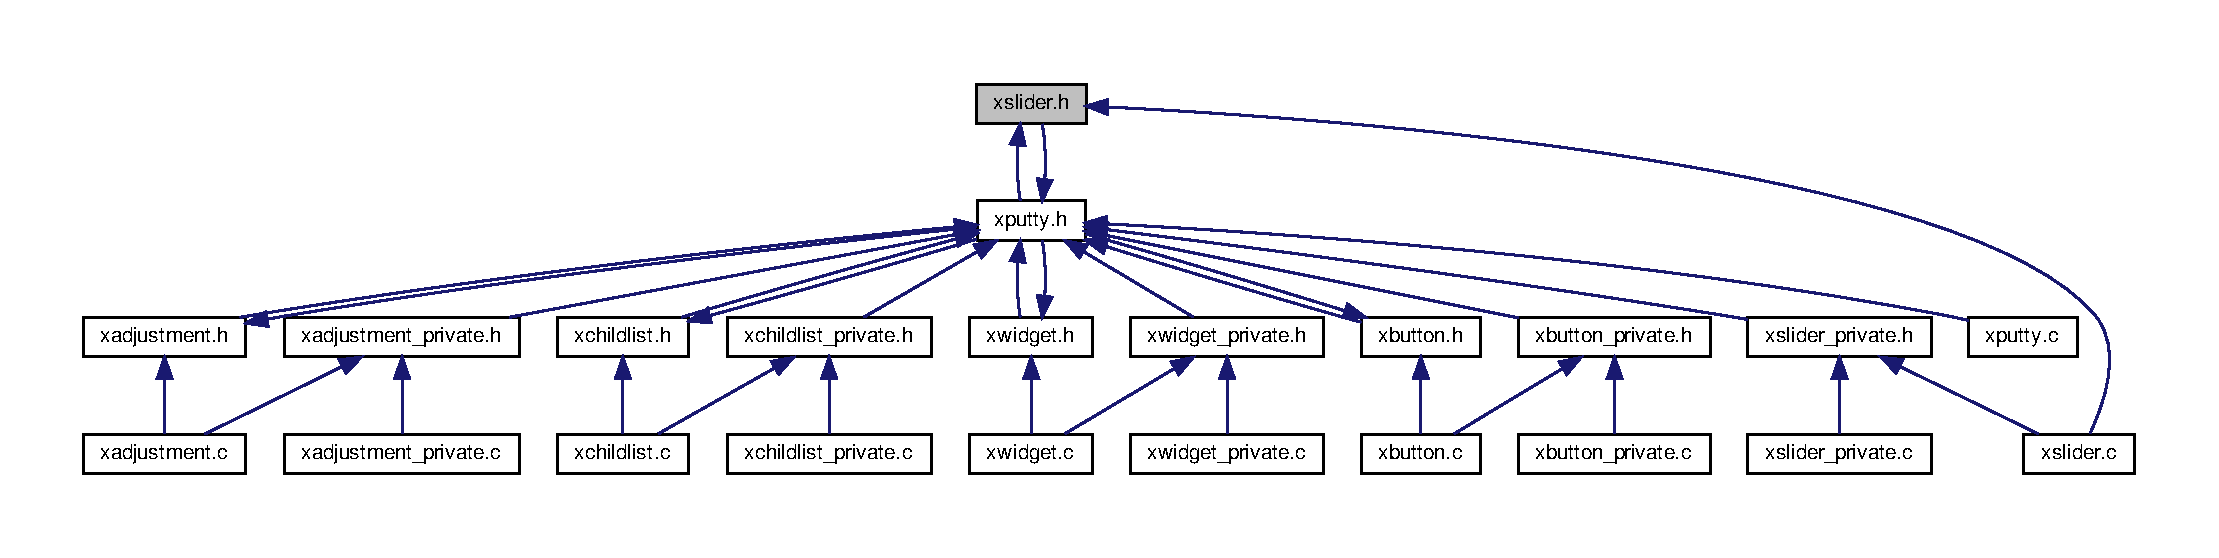
\includegraphics[width=350pt]{xslider_8h__dep__incl}
\end{center}
\end{figure}
\subsection*{Macros}
\begin{DoxyCompactItemize}
\item 
\#define \hyperlink{xslider_8h_a646859122e08747cbab6186ba07c51c1}{X\+S\+L\+I\+D\+E\+R\+\_\+\+H\+\_\+}
\end{DoxyCompactItemize}
\subsection*{Functions}
\begin{DoxyCompactItemize}
\item 
\hyperlink{structWidget__t}{Widget\+\_\+t} $\ast$ \hyperlink{xslider_8h_a80c7eeb4a1b25c6fcb855d407d959b48}{add\+\_\+vslider} (\hyperlink{structWidget__t}{Widget\+\_\+t} $\ast$parent, const char $\ast$label, int x, int y, int width, int height)
\begin{DoxyCompactList}\small\item\em add\+\_\+vslider -\/ add a vertical slider to a \hyperlink{structWidget__t}{Widget\+\_\+t} connect to func.\+value\+\_\+changed\+\_\+callback to implement your actions use set\+\_\+adjustment(w-\/$>$adj\+\_\+y, . . ) to set the range you need \end{DoxyCompactList}\item 
\hyperlink{structWidget__t}{Widget\+\_\+t} $\ast$ \hyperlink{xslider_8h_a508d0eea38b9c3a8b1e769b0e502c5bc}{add\+\_\+hslider} (\hyperlink{structWidget__t}{Widget\+\_\+t} $\ast$parent, const char $\ast$label, int x, int y, int width, int height)
\begin{DoxyCompactList}\small\item\em add\+\_\+hslider -\/ add a horizontal slider to a \hyperlink{structWidget__t}{Widget\+\_\+t} connect to func.\+value\+\_\+changed\+\_\+callback to implement your actions use set\+\_\+adjustment(w-\/$>$adj\+\_\+x, . . ) to set the range you need \end{DoxyCompactList}\end{DoxyCompactItemize}


\subsection{Macro Definition Documentation}
\mbox{\Hypertarget{xslider_8h_a646859122e08747cbab6186ba07c51c1}\label{xslider_8h_a646859122e08747cbab6186ba07c51c1}} 
\index{xslider.\+h@{xslider.\+h}!X\+S\+L\+I\+D\+E\+R\+\_\+\+H\+\_\+@{X\+S\+L\+I\+D\+E\+R\+\_\+\+H\+\_\+}}
\index{X\+S\+L\+I\+D\+E\+R\+\_\+\+H\+\_\+@{X\+S\+L\+I\+D\+E\+R\+\_\+\+H\+\_\+}!xslider.\+h@{xslider.\+h}}
\subsubsection{\texorpdfstring{X\+S\+L\+I\+D\+E\+R\+\_\+\+H\+\_\+}{XSLIDER\_H\_}}
{\footnotesize\ttfamily \#define X\+S\+L\+I\+D\+E\+R\+\_\+\+H\+\_\+}



\subsection{Function Documentation}
\mbox{\Hypertarget{xslider_8h_a508d0eea38b9c3a8b1e769b0e502c5bc}\label{xslider_8h_a508d0eea38b9c3a8b1e769b0e502c5bc}} 
\index{xslider.\+h@{xslider.\+h}!add\+\_\+hslider@{add\+\_\+hslider}}
\index{add\+\_\+hslider@{add\+\_\+hslider}!xslider.\+h@{xslider.\+h}}
\subsubsection{\texorpdfstring{add\+\_\+hslider()}{add\_hslider()}}
{\footnotesize\ttfamily \hyperlink{structWidget__t}{Widget\+\_\+t}$\ast$ add\+\_\+hslider (\begin{DoxyParamCaption}\item[{\hyperlink{structWidget__t}{Widget\+\_\+t} $\ast$}]{parent,  }\item[{const char $\ast$}]{label,  }\item[{int}]{x,  }\item[{int}]{y,  }\item[{int}]{width,  }\item[{int}]{height }\end{DoxyParamCaption})}



add\+\_\+hslider -\/ add a horizontal slider to a \hyperlink{structWidget__t}{Widget\+\_\+t} connect to func.\+value\+\_\+changed\+\_\+callback to implement your actions use set\+\_\+adjustment(w-\/$>$adj\+\_\+x, . . ) to set the range you need 


\begin{DoxyParams}{Parameters}
{\em $\ast$parent} & -\/ pointer to the \hyperlink{structWidget__t}{Widget\+\_\+t} request the button \\
\hline
{\em $\ast$label} & -\/ Label to show on the button \\
\hline
{\em x,y,width,height} & -\/ the position/geometry to create the button \\
\hline
\end{DoxyParams}
\begin{DoxyReturn}{Returns}
Widget\+\_\+t$\ast$ -\/ pointer to the \hyperlink{structWidget__t}{Widget\+\_\+t} button struct
\end{DoxyReturn}
add\+\_\+hslider -\/ add a horizontal slider to a \hyperlink{structWidget__t}{Widget\+\_\+t} connect to func.\+value\+\_\+changed\+\_\+callback to implement your actions use set\+\_\+adjustment(w-\/$>$adj\+\_\+x, . . ) to set the range you need


\begin{DoxyParams}{Parameters}
{\em $\ast$parent} & -\/ pointer to the \hyperlink{structWidget__t}{Widget\+\_\+t} request the button \\
\hline
{\em $\ast$label} & -\/ Label to show on the button \\
\hline
{\em x,y,width,height} & -\/ the position/geometry to create the button \\
\hline
\end{DoxyParams}
\begin{DoxyReturn}{Returns}
Widget\+\_\+t$\ast$ -\/ pointer to the \hyperlink{structWidget__t}{Widget\+\_\+t} button struct 
\end{DoxyReturn}
\mbox{\Hypertarget{xslider_8h_a80c7eeb4a1b25c6fcb855d407d959b48}\label{xslider_8h_a80c7eeb4a1b25c6fcb855d407d959b48}} 
\index{xslider.\+h@{xslider.\+h}!add\+\_\+vslider@{add\+\_\+vslider}}
\index{add\+\_\+vslider@{add\+\_\+vslider}!xslider.\+h@{xslider.\+h}}
\subsubsection{\texorpdfstring{add\+\_\+vslider()}{add\_vslider()}}
{\footnotesize\ttfamily \hyperlink{structWidget__t}{Widget\+\_\+t}$\ast$ add\+\_\+vslider (\begin{DoxyParamCaption}\item[{\hyperlink{structWidget__t}{Widget\+\_\+t} $\ast$}]{parent,  }\item[{const char $\ast$}]{label,  }\item[{int}]{x,  }\item[{int}]{y,  }\item[{int}]{width,  }\item[{int}]{height }\end{DoxyParamCaption})}



add\+\_\+vslider -\/ add a vertical slider to a \hyperlink{structWidget__t}{Widget\+\_\+t} connect to func.\+value\+\_\+changed\+\_\+callback to implement your actions use set\+\_\+adjustment(w-\/$>$adj\+\_\+y, . . ) to set the range you need 


\begin{DoxyParams}{Parameters}
{\em $\ast$parent} & -\/ pointer to the \hyperlink{structWidget__t}{Widget\+\_\+t} request the button \\
\hline
{\em $\ast$label} & -\/ Label to show on the button \\
\hline
{\em x,y,width,height} & -\/ the position/geometry to create the button \\
\hline
\end{DoxyParams}
\begin{DoxyReturn}{Returns}
Widget\+\_\+t$\ast$ -\/ pointer to the \hyperlink{structWidget__t}{Widget\+\_\+t} button struct
\end{DoxyReturn}
add\+\_\+vslider -\/ add a vertical slider to a \hyperlink{structWidget__t}{Widget\+\_\+t} connect to func.\+value\+\_\+changed\+\_\+callback to implement your actions use set\+\_\+adjustment(w-\/$>$adj\+\_\+y, . . ) to set the range you need


\begin{DoxyParams}{Parameters}
{\em $\ast$parent} & -\/ pointer to the \hyperlink{structWidget__t}{Widget\+\_\+t} request the button \\
\hline
{\em $\ast$label} & -\/ Label to show on the button \\
\hline
{\em x,y,width,height} & -\/ the position/geometry to create the button \\
\hline
\end{DoxyParams}
\begin{DoxyReturn}{Returns}
Widget\+\_\+t$\ast$ -\/ pointer to the \hyperlink{structWidget__t}{Widget\+\_\+t} button struct 
\end{DoxyReturn}

\hypertarget{xslider__private_8c}{}\section{xslider\+\_\+private.\+c File Reference}
\label{xslider__private_8c}\index{xslider\+\_\+private.\+c@{xslider\+\_\+private.\+c}}
{\ttfamily \#include \char`\"{}xslider\+\_\+private.\+h\char`\"{}}\newline
Include dependency graph for xslider\+\_\+private.\+c\+:
\nopagebreak
\begin{figure}[H]
\begin{center}
\leavevmode
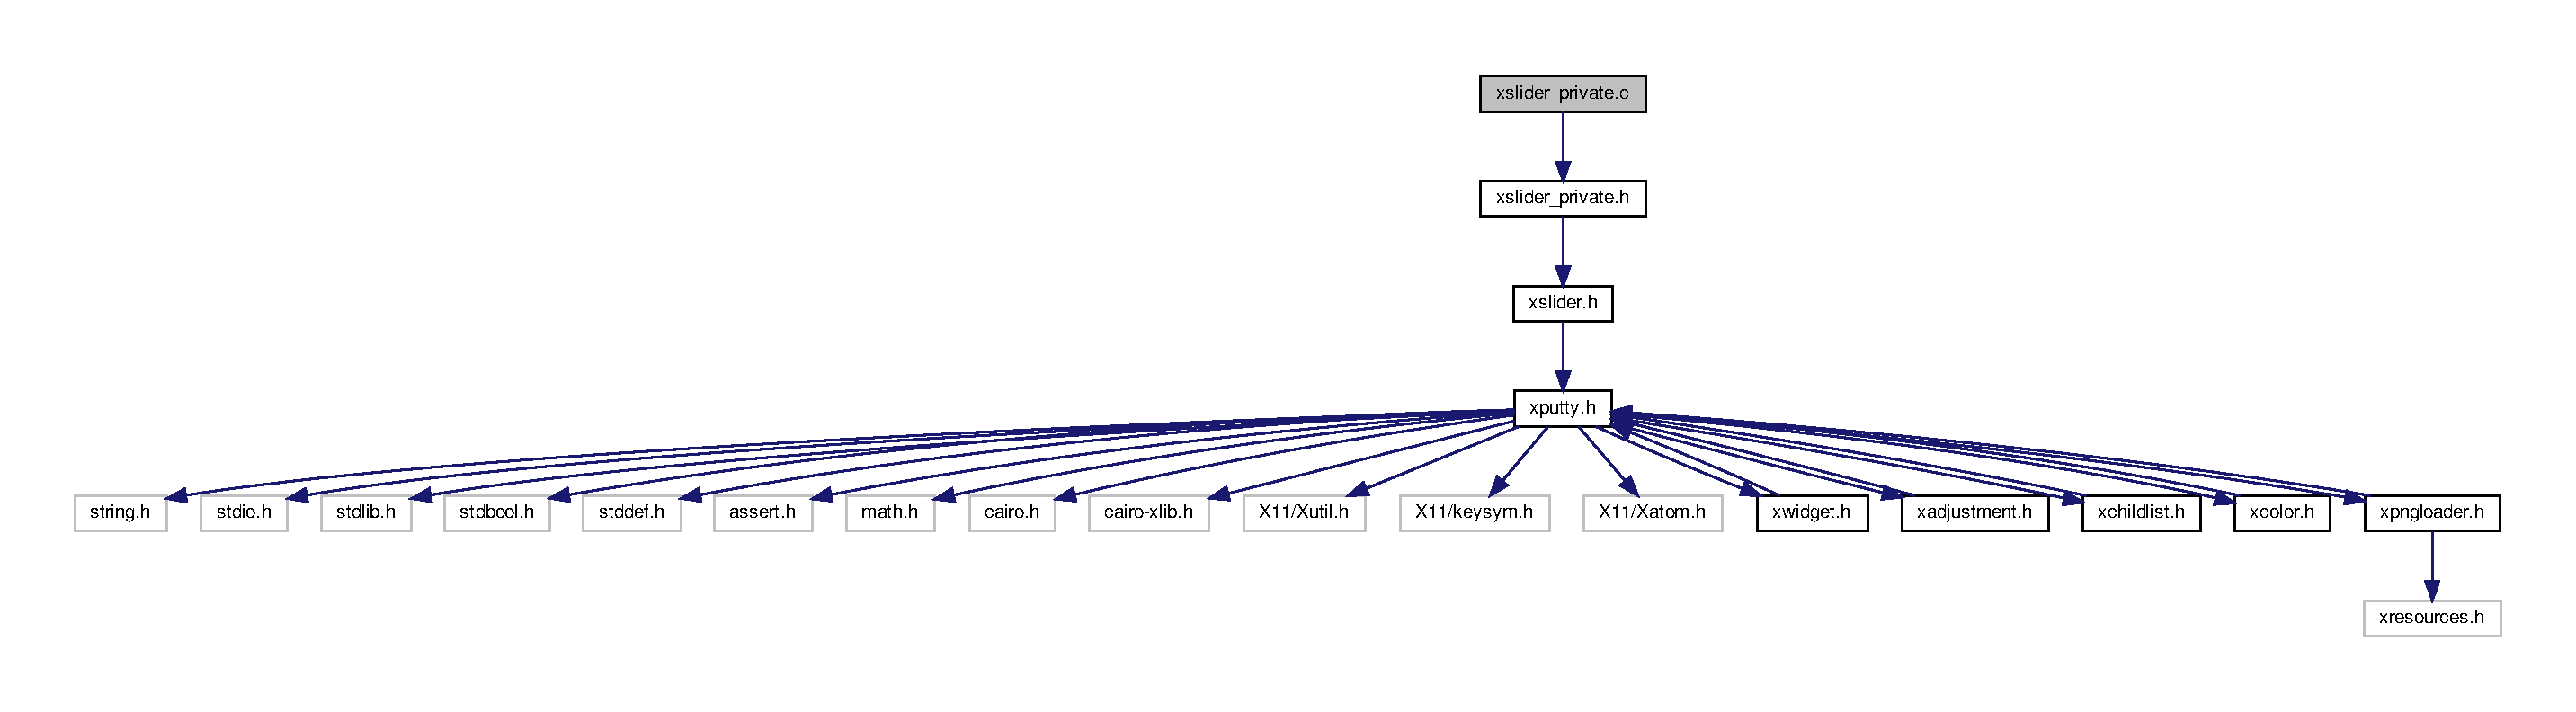
\includegraphics[width=350pt]{xslider__private_8c__incl}
\end{center}
\end{figure}
\subsection*{Functions}
\begin{DoxyCompactItemize}
\item 
void \hyperlink{xslider__private_8c_af5a5ea0246cbb2770232525d99587434}{\+\_\+pattern\+\_\+vslider} (\hyperlink{structWidget__t}{Widget\+\_\+t} $\ast$w, \hyperlink{xwidget_8h_a8a9a00ba3976b54d9c5cacffe16d14ef}{Widget\+\_\+state} st, int width)
\begin{DoxyCompactList}\small\item\em \+\_\+pattern\+\_\+vslider -\/ set pattern for the slider base \end{DoxyCompactList}\item 
void \hyperlink{xslider__private_8c_a3c1cb4b0d95613749744030231daa3b8}{\+\_\+pattern\+\_\+hslider} (\hyperlink{structWidget__t}{Widget\+\_\+t} $\ast$w, \hyperlink{xwidget_8h_a8a9a00ba3976b54d9c5cacffe16d14ef}{Widget\+\_\+state} st, int height)
\begin{DoxyCompactList}\small\item\em \+\_\+pattern\+\_\+hslider -\/ set pattern for the slider base \end{DoxyCompactList}\item 
void \hyperlink{xslider__private_8c_a9c331bf737e3d50daa109a4a74585315}{\+\_\+draw\+\_\+vslider} (void $\ast$w\+\_\+, void $\ast$user\+\_\+data)
\begin{DoxyCompactList}\small\item\em \+\_\+draw\+\_\+vslider -\/ internal draw the slider to the buffer \end{DoxyCompactList}\item 
void \hyperlink{xslider__private_8c_a65b279b4fc239e85326dfd50e65b6574}{\+\_\+draw\+\_\+hslider} (void $\ast$w\+\_\+, void $\ast$user\+\_\+data)
\begin{DoxyCompactList}\small\item\em \+\_\+draw\+\_\+hslider -\/ internal draw the slider to the buffer \end{DoxyCompactList}\item 
void \hyperlink{xslider__private_8c_a15a2fae4b8325b037644afb6131827b5}{\+\_\+slider\+\_\+released} (void $\ast$w\+\_\+, void $\ast$button\+\_\+, void $\ast$user\+\_\+data)
\begin{DoxyCompactList}\small\item\em \+\_\+slider\+\_\+released -\/ redraw the slider when buttob released \end{DoxyCompactList}\end{DoxyCompactItemize}


\subsection{Function Documentation}
\mbox{\Hypertarget{xslider__private_8c_a65b279b4fc239e85326dfd50e65b6574}\label{xslider__private_8c_a65b279b4fc239e85326dfd50e65b6574}} 
\index{xslider\+\_\+private.\+c@{xslider\+\_\+private.\+c}!\+\_\+draw\+\_\+hslider@{\+\_\+draw\+\_\+hslider}}
\index{\+\_\+draw\+\_\+hslider@{\+\_\+draw\+\_\+hslider}!xslider\+\_\+private.\+c@{xslider\+\_\+private.\+c}}
\subsubsection{\texorpdfstring{\+\_\+draw\+\_\+hslider()}{\_draw\_hslider()}}
{\footnotesize\ttfamily void \+\_\+draw\+\_\+hslider (\begin{DoxyParamCaption}\item[{void $\ast$}]{w\+\_\+,  }\item[{void $\ast$}]{user\+\_\+data }\end{DoxyParamCaption})}



\+\_\+draw\+\_\+hslider -\/ internal draw the slider to the buffer 


\begin{DoxyParams}{Parameters}
{\em $\ast$w\+\_\+} & -\/ void pointer to the \hyperlink{structWidget__t}{Widget\+\_\+t} button \\
\hline
{\em $\ast$user\+\_\+data} & -\/ void pointer to attached user\+\_\+data \\
\hline
\end{DoxyParams}
\begin{DoxyReturn}{Returns}
void 
\end{DoxyReturn}
\mbox{\Hypertarget{xslider__private_8c_a9c331bf737e3d50daa109a4a74585315}\label{xslider__private_8c_a9c331bf737e3d50daa109a4a74585315}} 
\index{xslider\+\_\+private.\+c@{xslider\+\_\+private.\+c}!\+\_\+draw\+\_\+vslider@{\+\_\+draw\+\_\+vslider}}
\index{\+\_\+draw\+\_\+vslider@{\+\_\+draw\+\_\+vslider}!xslider\+\_\+private.\+c@{xslider\+\_\+private.\+c}}
\subsubsection{\texorpdfstring{\+\_\+draw\+\_\+vslider()}{\_draw\_vslider()}}
{\footnotesize\ttfamily void \+\_\+draw\+\_\+vslider (\begin{DoxyParamCaption}\item[{void $\ast$}]{w\+\_\+,  }\item[{void $\ast$}]{user\+\_\+data }\end{DoxyParamCaption})}



\+\_\+draw\+\_\+vslider -\/ internal draw the slider to the buffer 


\begin{DoxyParams}{Parameters}
{\em $\ast$w\+\_\+} & -\/ void pointer to the \hyperlink{structWidget__t}{Widget\+\_\+t} button \\
\hline
{\em $\ast$user\+\_\+data} & -\/ void pointer to attached user\+\_\+data \\
\hline
\end{DoxyParams}
\begin{DoxyReturn}{Returns}
void 
\end{DoxyReturn}
\mbox{\Hypertarget{xslider__private_8c_a3c1cb4b0d95613749744030231daa3b8}\label{xslider__private_8c_a3c1cb4b0d95613749744030231daa3b8}} 
\index{xslider\+\_\+private.\+c@{xslider\+\_\+private.\+c}!\+\_\+pattern\+\_\+hslider@{\+\_\+pattern\+\_\+hslider}}
\index{\+\_\+pattern\+\_\+hslider@{\+\_\+pattern\+\_\+hslider}!xslider\+\_\+private.\+c@{xslider\+\_\+private.\+c}}
\subsubsection{\texorpdfstring{\+\_\+pattern\+\_\+hslider()}{\_pattern\_hslider()}}
{\footnotesize\ttfamily void \+\_\+pattern\+\_\+hslider (\begin{DoxyParamCaption}\item[{\hyperlink{structWidget__t}{Widget\+\_\+t} $\ast$}]{w,  }\item[{\hyperlink{xwidget_8h_a8a9a00ba3976b54d9c5cacffe16d14ef}{Widget\+\_\+state}}]{st,  }\item[{int}]{height }\end{DoxyParamCaption})}



\+\_\+pattern\+\_\+hslider -\/ set pattern for the slider base 


\begin{DoxyParams}{Parameters}
{\em $\ast$w\+\_\+} & -\/ void pointer to the \hyperlink{structWidget__t}{Widget\+\_\+t} button \\
\hline
{\em st} & -\/ the \hyperlink{structWidget__t}{Widget\+\_\+t} \hyperlink{structColor__t}{Color\+\_\+t} mode to use \\
\hline
{\em width} & -\/ the width of the base \\
\hline
\end{DoxyParams}
\begin{DoxyReturn}{Returns}
void 
\end{DoxyReturn}
\mbox{\Hypertarget{xslider__private_8c_af5a5ea0246cbb2770232525d99587434}\label{xslider__private_8c_af5a5ea0246cbb2770232525d99587434}} 
\index{xslider\+\_\+private.\+c@{xslider\+\_\+private.\+c}!\+\_\+pattern\+\_\+vslider@{\+\_\+pattern\+\_\+vslider}}
\index{\+\_\+pattern\+\_\+vslider@{\+\_\+pattern\+\_\+vslider}!xslider\+\_\+private.\+c@{xslider\+\_\+private.\+c}}
\subsubsection{\texorpdfstring{\+\_\+pattern\+\_\+vslider()}{\_pattern\_vslider()}}
{\footnotesize\ttfamily void \+\_\+pattern\+\_\+vslider (\begin{DoxyParamCaption}\item[{\hyperlink{structWidget__t}{Widget\+\_\+t} $\ast$}]{w,  }\item[{\hyperlink{xwidget_8h_a8a9a00ba3976b54d9c5cacffe16d14ef}{Widget\+\_\+state}}]{st,  }\item[{int}]{width }\end{DoxyParamCaption})}



\+\_\+pattern\+\_\+vslider -\/ set pattern for the slider base 


\begin{DoxyParams}{Parameters}
{\em $\ast$w\+\_\+} & -\/ void pointer to the \hyperlink{structWidget__t}{Widget\+\_\+t} button \\
\hline
{\em st} & -\/ the \hyperlink{structWidget__t}{Widget\+\_\+t} \hyperlink{structColor__t}{Color\+\_\+t} mode to use \\
\hline
{\em width} & -\/ the width of the base \\
\hline
\end{DoxyParams}
\begin{DoxyReturn}{Returns}
void 
\end{DoxyReturn}
\mbox{\Hypertarget{xslider__private_8c_a15a2fae4b8325b037644afb6131827b5}\label{xslider__private_8c_a15a2fae4b8325b037644afb6131827b5}} 
\index{xslider\+\_\+private.\+c@{xslider\+\_\+private.\+c}!\+\_\+slider\+\_\+released@{\+\_\+slider\+\_\+released}}
\index{\+\_\+slider\+\_\+released@{\+\_\+slider\+\_\+released}!xslider\+\_\+private.\+c@{xslider\+\_\+private.\+c}}
\subsubsection{\texorpdfstring{\+\_\+slider\+\_\+released()}{\_slider\_released()}}
{\footnotesize\ttfamily void \+\_\+slider\+\_\+released (\begin{DoxyParamCaption}\item[{void $\ast$}]{w\+\_\+,  }\item[{void $\ast$}]{button\+\_\+,  }\item[{void $\ast$}]{user\+\_\+data }\end{DoxyParamCaption})}



\+\_\+slider\+\_\+released -\/ redraw the slider when buttob released 


\begin{DoxyParams}{Parameters}
{\em $\ast$w\+\_\+} & -\/ void pointer to the \hyperlink{structWidget__t}{Widget\+\_\+t} button \\
\hline
{\em $\ast$user\+\_\+data} & -\/ void pointer to attached user\+\_\+data \\
\hline
\end{DoxyParams}
\begin{DoxyReturn}{Returns}
void 
\end{DoxyReturn}

\hypertarget{xslider__private_8h}{}\section{xslider\+\_\+private.\+h File Reference}
\label{xslider__private_8h}\index{xslider\+\_\+private.\+h@{xslider\+\_\+private.\+h}}
{\ttfamily \#include \char`\"{}xputty.\+h\char`\"{}}\newline
Include dependency graph for xslider\+\_\+private.\+h\+:
\nopagebreak
\begin{figure}[H]
\begin{center}
\leavevmode
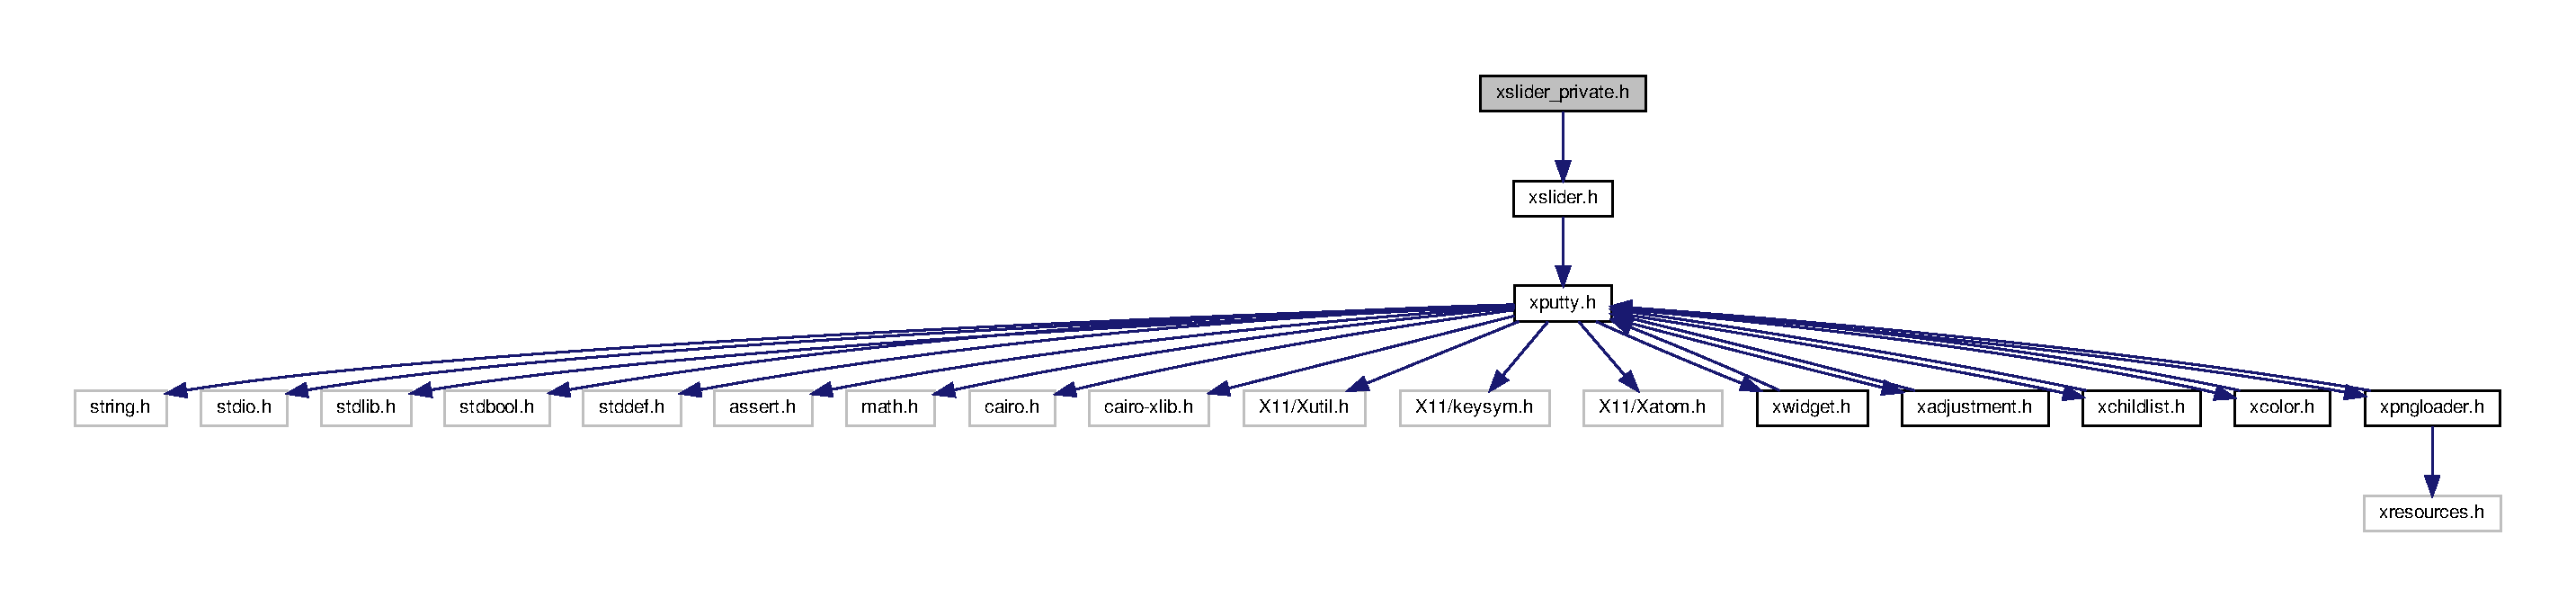
\includegraphics[width=350pt]{xslider__private_8h__incl}
\end{center}
\end{figure}
This graph shows which files directly or indirectly include this file\+:
\nopagebreak
\begin{figure}[H]
\begin{center}
\leavevmode
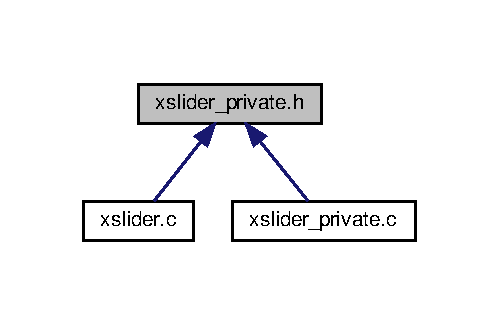
\includegraphics[width=240pt]{xslider__private_8h__dep__incl}
\end{center}
\end{figure}
\subsection*{Macros}
\begin{DoxyCompactItemize}
\item 
\#define \hyperlink{xslider__private_8h_ab6e5db46601e79b070042cb2f5caa589}{X\+S\+L\+I\+D\+E\+R\+\_\+\+P\+R\+I\+V\+A\+T\+E\+\_\+\+H\+\_\+}
\end{DoxyCompactItemize}
\subsection*{Functions}
\begin{DoxyCompactItemize}
\item 
void \hyperlink{xslider__private_8h_afbd00aa98160ecad075c7378e6a53c74}{\+\_\+pattern\+\_\+vslider} (\hyperlink{structWidget__t}{Widget\+\_\+t} $\ast$w, \hyperlink{xcolor_8h_af6e1bc675d5df2f7fb9e91a8c5820771}{Color\+\_\+state} st, int width)
\begin{DoxyCompactList}\small\item\em \+\_\+pattern\+\_\+vslider -\/ set pattern for the slider base \end{DoxyCompactList}\item 
void \hyperlink{xslider__private_8h_ae0dfcbeb4edf64bd460e8961fc5ca668}{\+\_\+pattern\+\_\+hslider} (\hyperlink{structWidget__t}{Widget\+\_\+t} $\ast$w, \hyperlink{xcolor_8h_af6e1bc675d5df2f7fb9e91a8c5820771}{Color\+\_\+state} st, int width)
\begin{DoxyCompactList}\small\item\em \+\_\+pattern\+\_\+hslider -\/ set pattern for the slider base \end{DoxyCompactList}\item 
void \hyperlink{xslider__private_8h_a9c331bf737e3d50daa109a4a74585315}{\+\_\+draw\+\_\+vslider} (void $\ast$w\+\_\+, void $\ast$user\+\_\+data)
\begin{DoxyCompactList}\small\item\em \+\_\+draw\+\_\+vslider -\/ internal draw the slider to the buffer \end{DoxyCompactList}\item 
void \hyperlink{xslider__private_8h_a65b279b4fc239e85326dfd50e65b6574}{\+\_\+draw\+\_\+hslider} (void $\ast$w\+\_\+, void $\ast$user\+\_\+data)
\begin{DoxyCompactList}\small\item\em \+\_\+draw\+\_\+hslider -\/ internal draw the slider to the buffer \end{DoxyCompactList}\item 
void \hyperlink{xslider__private_8h_a15a2fae4b8325b037644afb6131827b5}{\+\_\+slider\+\_\+released} (void $\ast$w\+\_\+, void $\ast$button\+\_\+, void $\ast$user\+\_\+data)
\begin{DoxyCompactList}\small\item\em \+\_\+slider\+\_\+released -\/ redraw the slider when buttob released \end{DoxyCompactList}\end{DoxyCompactItemize}


\subsection{Macro Definition Documentation}
\mbox{\Hypertarget{xslider__private_8h_ab6e5db46601e79b070042cb2f5caa589}\label{xslider__private_8h_ab6e5db46601e79b070042cb2f5caa589}} 
\index{xslider\+\_\+private.\+h@{xslider\+\_\+private.\+h}!X\+S\+L\+I\+D\+E\+R\+\_\+\+P\+R\+I\+V\+A\+T\+E\+\_\+\+H\+\_\+@{X\+S\+L\+I\+D\+E\+R\+\_\+\+P\+R\+I\+V\+A\+T\+E\+\_\+\+H\+\_\+}}
\index{X\+S\+L\+I\+D\+E\+R\+\_\+\+P\+R\+I\+V\+A\+T\+E\+\_\+\+H\+\_\+@{X\+S\+L\+I\+D\+E\+R\+\_\+\+P\+R\+I\+V\+A\+T\+E\+\_\+\+H\+\_\+}!xslider\+\_\+private.\+h@{xslider\+\_\+private.\+h}}
\subsubsection{\texorpdfstring{X\+S\+L\+I\+D\+E\+R\+\_\+\+P\+R\+I\+V\+A\+T\+E\+\_\+\+H\+\_\+}{XSLIDER\_PRIVATE\_H\_}}
{\footnotesize\ttfamily \#define X\+S\+L\+I\+D\+E\+R\+\_\+\+P\+R\+I\+V\+A\+T\+E\+\_\+\+H\+\_\+}



\subsection{Function Documentation}
\mbox{\Hypertarget{xslider__private_8h_a65b279b4fc239e85326dfd50e65b6574}\label{xslider__private_8h_a65b279b4fc239e85326dfd50e65b6574}} 
\index{xslider\+\_\+private.\+h@{xslider\+\_\+private.\+h}!\+\_\+draw\+\_\+hslider@{\+\_\+draw\+\_\+hslider}}
\index{\+\_\+draw\+\_\+hslider@{\+\_\+draw\+\_\+hslider}!xslider\+\_\+private.\+h@{xslider\+\_\+private.\+h}}
\subsubsection{\texorpdfstring{\+\_\+draw\+\_\+hslider()}{\_draw\_hslider()}}
{\footnotesize\ttfamily void \+\_\+draw\+\_\+hslider (\begin{DoxyParamCaption}\item[{void $\ast$}]{w\+\_\+,  }\item[{void $\ast$}]{user\+\_\+data }\end{DoxyParamCaption})}



\+\_\+draw\+\_\+hslider -\/ internal draw the slider to the buffer 


\begin{DoxyParams}{Parameters}
{\em $\ast$w\+\_\+} & -\/ void pointer to the \hyperlink{structWidget__t}{Widget\+\_\+t} button \\
\hline
{\em $\ast$user\+\_\+data} & -\/ void pointer to attached user\+\_\+data \\
\hline
\end{DoxyParams}
\begin{DoxyReturn}{Returns}
void 
\end{DoxyReturn}
\mbox{\Hypertarget{xslider__private_8h_a9c331bf737e3d50daa109a4a74585315}\label{xslider__private_8h_a9c331bf737e3d50daa109a4a74585315}} 
\index{xslider\+\_\+private.\+h@{xslider\+\_\+private.\+h}!\+\_\+draw\+\_\+vslider@{\+\_\+draw\+\_\+vslider}}
\index{\+\_\+draw\+\_\+vslider@{\+\_\+draw\+\_\+vslider}!xslider\+\_\+private.\+h@{xslider\+\_\+private.\+h}}
\subsubsection{\texorpdfstring{\+\_\+draw\+\_\+vslider()}{\_draw\_vslider()}}
{\footnotesize\ttfamily void \+\_\+draw\+\_\+vslider (\begin{DoxyParamCaption}\item[{void $\ast$}]{w\+\_\+,  }\item[{void $\ast$}]{user\+\_\+data }\end{DoxyParamCaption})}



\+\_\+draw\+\_\+vslider -\/ internal draw the slider to the buffer 


\begin{DoxyParams}{Parameters}
{\em $\ast$w\+\_\+} & -\/ void pointer to the \hyperlink{structWidget__t}{Widget\+\_\+t} button \\
\hline
{\em $\ast$user\+\_\+data} & -\/ void pointer to attached user\+\_\+data \\
\hline
\end{DoxyParams}
\begin{DoxyReturn}{Returns}
void 
\end{DoxyReturn}
\mbox{\Hypertarget{xslider__private_8h_ae0dfcbeb4edf64bd460e8961fc5ca668}\label{xslider__private_8h_ae0dfcbeb4edf64bd460e8961fc5ca668}} 
\index{xslider\+\_\+private.\+h@{xslider\+\_\+private.\+h}!\+\_\+pattern\+\_\+hslider@{\+\_\+pattern\+\_\+hslider}}
\index{\+\_\+pattern\+\_\+hslider@{\+\_\+pattern\+\_\+hslider}!xslider\+\_\+private.\+h@{xslider\+\_\+private.\+h}}
\subsubsection{\texorpdfstring{\+\_\+pattern\+\_\+hslider()}{\_pattern\_hslider()}}
{\footnotesize\ttfamily void \+\_\+pattern\+\_\+hslider (\begin{DoxyParamCaption}\item[{\hyperlink{structWidget__t}{Widget\+\_\+t} $\ast$}]{w,  }\item[{\hyperlink{xcolor_8h_af6e1bc675d5df2f7fb9e91a8c5820771}{Color\+\_\+state}}]{st,  }\item[{int}]{height }\end{DoxyParamCaption})}



\+\_\+pattern\+\_\+hslider -\/ set pattern for the slider base 


\begin{DoxyParams}{Parameters}
{\em $\ast$w\+\_\+} & -\/ void pointer to the \hyperlink{structWidget__t}{Widget\+\_\+t} button \\
\hline
{\em st} & -\/ the \hyperlink{structWidget__t}{Widget\+\_\+t} Color\+\_\+t mode to use \\
\hline
{\em width} & -\/ the width of the base \\
\hline
\end{DoxyParams}
\begin{DoxyReturn}{Returns}
void 
\end{DoxyReturn}
\mbox{\Hypertarget{xslider__private_8h_afbd00aa98160ecad075c7378e6a53c74}\label{xslider__private_8h_afbd00aa98160ecad075c7378e6a53c74}} 
\index{xslider\+\_\+private.\+h@{xslider\+\_\+private.\+h}!\+\_\+pattern\+\_\+vslider@{\+\_\+pattern\+\_\+vslider}}
\index{\+\_\+pattern\+\_\+vslider@{\+\_\+pattern\+\_\+vslider}!xslider\+\_\+private.\+h@{xslider\+\_\+private.\+h}}
\subsubsection{\texorpdfstring{\+\_\+pattern\+\_\+vslider()}{\_pattern\_vslider()}}
{\footnotesize\ttfamily void \+\_\+pattern\+\_\+vslider (\begin{DoxyParamCaption}\item[{\hyperlink{structWidget__t}{Widget\+\_\+t} $\ast$}]{w,  }\item[{\hyperlink{xcolor_8h_af6e1bc675d5df2f7fb9e91a8c5820771}{Color\+\_\+state}}]{st,  }\item[{int}]{width }\end{DoxyParamCaption})}



\+\_\+pattern\+\_\+vslider -\/ set pattern for the slider base 


\begin{DoxyParams}{Parameters}
{\em $\ast$w\+\_\+} & -\/ void pointer to the \hyperlink{structWidget__t}{Widget\+\_\+t} button \\
\hline
{\em st} & -\/ the \hyperlink{structWidget__t}{Widget\+\_\+t} Color\+\_\+t mode to use \\
\hline
{\em width} & -\/ the width of the base \\
\hline
\end{DoxyParams}
\begin{DoxyReturn}{Returns}
void 
\end{DoxyReturn}
\mbox{\Hypertarget{xslider__private_8h_a15a2fae4b8325b037644afb6131827b5}\label{xslider__private_8h_a15a2fae4b8325b037644afb6131827b5}} 
\index{xslider\+\_\+private.\+h@{xslider\+\_\+private.\+h}!\+\_\+slider\+\_\+released@{\+\_\+slider\+\_\+released}}
\index{\+\_\+slider\+\_\+released@{\+\_\+slider\+\_\+released}!xslider\+\_\+private.\+h@{xslider\+\_\+private.\+h}}
\subsubsection{\texorpdfstring{\+\_\+slider\+\_\+released()}{\_slider\_released()}}
{\footnotesize\ttfamily void \+\_\+slider\+\_\+released (\begin{DoxyParamCaption}\item[{void $\ast$}]{w\+\_\+,  }\item[{void $\ast$}]{button\+\_\+,  }\item[{void $\ast$}]{user\+\_\+data }\end{DoxyParamCaption})}



\+\_\+slider\+\_\+released -\/ redraw the slider when buttob released 


\begin{DoxyParams}{Parameters}
{\em $\ast$w\+\_\+} & -\/ void pointer to the \hyperlink{structWidget__t}{Widget\+\_\+t} button \\
\hline
{\em $\ast$user\+\_\+data} & -\/ void pointer to attached user\+\_\+data \\
\hline
\end{DoxyParams}
\begin{DoxyReturn}{Returns}
void 
\end{DoxyReturn}

\hypertarget{xwidget_8c}{}\section{xwidget.\+c File Reference}
\label{xwidget_8c}\index{xwidget.\+c@{xwidget.\+c}}
{\ttfamily \#include \char`\"{}xwidget.\+h\char`\"{}}\newline
Include dependency graph for xwidget.\+c\+:
\nopagebreak
\begin{figure}[H]
\begin{center}
\leavevmode
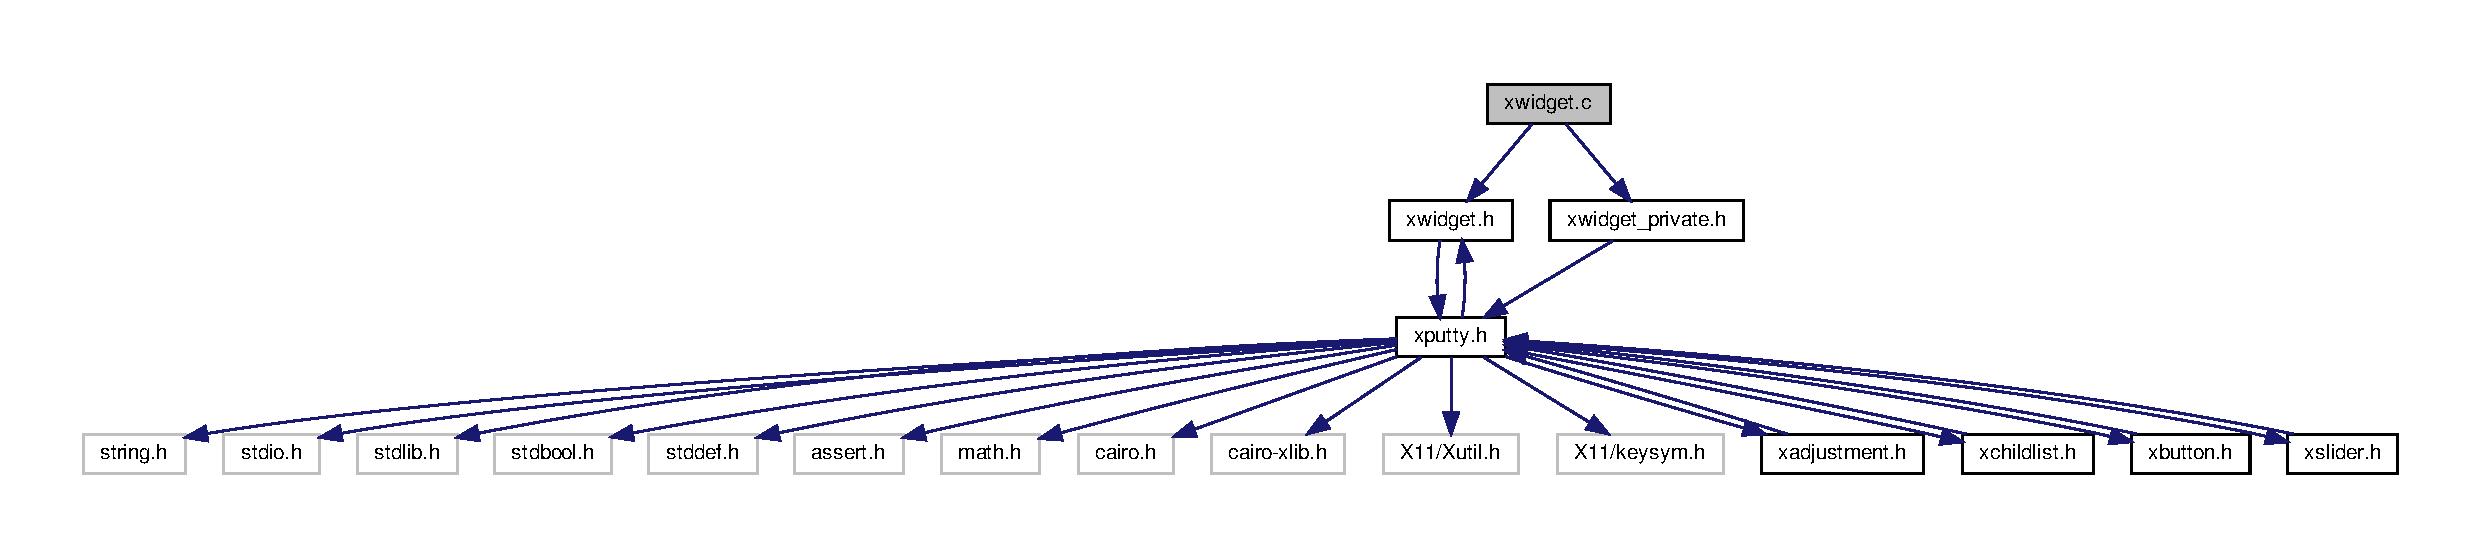
\includegraphics[width=350pt]{xwidget_8c__incl}
\end{center}
\end{figure}
\subsection*{Functions}
\begin{DoxyCompactItemize}
\item 
int \hyperlink{xwidget_8c_a1607cf4a642a38ea235a007ea9579403}{key\+\_\+mapping} (Display $\ast$dpy, X\+Key\+Event $\ast$xkey)
\begin{DoxyCompactList}\small\item\em key\+\_\+mapping -\/ modifier key\textquotesingle{}s mapped to a integer value \end{DoxyCompactList}\item 
void \hyperlink{xwidget_8c_a540b0eefd6f19f487aa71d4c1798ac8c}{destroy\+\_\+widget} (\hyperlink{structWidget__t}{Widget\+\_\+t} $\ast$w, X\+Context Context)
\begin{DoxyCompactList}\small\item\em destroy\+\_\+widget -\/ destroy a widget and remove it from the Context \end{DoxyCompactList}\item 
void \hyperlink{xwidget_8c_acf8c7ef79c60253a687116d3783e1c67}{configure\+\_\+event} (void $\ast$w\+\_\+, void $\ast$user\+\_\+data)
\begin{DoxyCompactList}\small\item\em configure\+\_\+event -\/ default callback when a widget receive a Configure\+Notify \end{DoxyCompactList}\item 
\hyperlink{structWidget__t}{Widget\+\_\+t} $\ast$ \hyperlink{xwidget_8c_a9c5b8eaf662ac4fb7d2674bf7e89ab8c}{create\+\_\+window} (Display $\ast$dpy, Window win, X\+Context Context, int x, int y, int width, int height)
\begin{DoxyCompactList}\small\item\em $\ast$create\+\_\+window -\/ create a Window \end{DoxyCompactList}\item 
\hyperlink{structWidget__t}{Widget\+\_\+t} $\ast$ \hyperlink{xwidget_8c_a2eadb62cb8f0794ffa6251be77f8d1a1}{create\+\_\+widget} (Display $\ast$dpy, \hyperlink{structWidget__t}{Widget\+\_\+t} $\ast$parent, X\+Context Context, int x, int y, int width, int height)
\begin{DoxyCompactList}\small\item\em $\ast$create\+\_\+widget -\/ create a widget \end{DoxyCompactList}\item 
void \hyperlink{xwidget_8c_a0e801c1a701cc8526b198371ce2ff692}{transparent\+\_\+draw} (void $\ast$w\+\_\+, void $\ast$user\+\_\+data)
\begin{DoxyCompactList}\small\item\em transparent\+\_\+draw -\/ copy parent surface to child surface \end{DoxyCompactList}\item 
void \hyperlink{xwidget_8c_af3ecce0332b5f13b590d024db28aec5a}{widget\+\_\+event\+\_\+loop} (void $\ast$w\+\_\+, void $\ast$event, void $\ast$user\+\_\+data)
\begin{DoxyCompactList}\small\item\em widget\+\_\+event\+\_\+loop -\/ the internal widget event loop \end{DoxyCompactList}\item 
void \hyperlink{xwidget_8c_a4d835af5b56eb13ed7bd4602ce7ccd92}{quit} (\hyperlink{structWidget__t}{Widget\+\_\+t} $\ast$w)
\begin{DoxyCompactList}\small\item\em quit -\/ exit the main loop \end{DoxyCompactList}\item 
void \hyperlink{xwidget_8c_a5dc619d89042819195db7e744dcd5f7d}{loop} (\hyperlink{structWidget__t}{Widget\+\_\+t} $\ast$w, X\+Context context, bool $\ast$run)
\begin{DoxyCompactList}\small\item\em loop -\/ the event loop \end{DoxyCompactList}\end{DoxyCompactItemize}


\subsection{Function Documentation}
\mbox{\Hypertarget{xwidget_8c_acf8c7ef79c60253a687116d3783e1c67}\label{xwidget_8c_acf8c7ef79c60253a687116d3783e1c67}} 
\index{xwidget.\+c@{xwidget.\+c}!configure\+\_\+event@{configure\+\_\+event}}
\index{configure\+\_\+event@{configure\+\_\+event}!xwidget.\+c@{xwidget.\+c}}
\subsubsection{\texorpdfstring{configure\+\_\+event()}{configure\_event()}}
{\footnotesize\ttfamily void configure\+\_\+event (\begin{DoxyParamCaption}\item[{void $\ast$}]{w\+\_\+,  }\item[{void $\ast$}]{user\+\_\+data }\end{DoxyParamCaption})}



configure\+\_\+event -\/ default callback when a widget receive a Configure\+Notify 


\begin{DoxyParams}{Parameters}
{\em $\ast$w} & -\/ pointer to the \hyperlink{structWidget__t}{Widget\+\_\+t} receive the event \\
\hline
{\em user\+\_\+data} & -\/ void pointer to attached user\+\_\+data \\
\hline
\end{DoxyParams}
\begin{DoxyReturn}{Returns}
void 
\end{DoxyReturn}
\mbox{\Hypertarget{xwidget_8c_a2eadb62cb8f0794ffa6251be77f8d1a1}\label{xwidget_8c_a2eadb62cb8f0794ffa6251be77f8d1a1}} 
\index{xwidget.\+c@{xwidget.\+c}!create\+\_\+widget@{create\+\_\+widget}}
\index{create\+\_\+widget@{create\+\_\+widget}!xwidget.\+c@{xwidget.\+c}}
\subsubsection{\texorpdfstring{create\+\_\+widget()}{create\_widget()}}
{\footnotesize\ttfamily \hyperlink{structWidget__t}{Widget\+\_\+t}$\ast$ create\+\_\+widget (\begin{DoxyParamCaption}\item[{Display $\ast$}]{dpy,  }\item[{\hyperlink{structWidget__t}{Widget\+\_\+t} $\ast$}]{parent,  }\item[{X\+Context}]{Context,  }\item[{int}]{x,  }\item[{int}]{y,  }\item[{int}]{width,  }\item[{int}]{height }\end{DoxyParamCaption})}



$\ast$create\+\_\+widget -\/ create a widget 


\begin{DoxyParams}{Parameters}
{\em $\ast$dpy} & -\/ pointer to the Display to use \\
\hline
{\em $\ast$parent} & -\/ pointer to the Parrent \hyperlink{structWidget__t}{Widget\+\_\+t} \\
\hline
{\em Context} & -\/ a X\+Context to store Window informations \\
\hline
{\em x,y,width,height} & -\/ the position/geometry to create the widget \\
\hline
\end{DoxyParams}
\begin{DoxyReturn}{Returns}
Widget\+\_\+t$\ast$ -\/ pointer to the \hyperlink{structWidget__t}{Widget\+\_\+t} struct 
\end{DoxyReturn}
\mbox{\Hypertarget{xwidget_8c_a9c5b8eaf662ac4fb7d2674bf7e89ab8c}\label{xwidget_8c_a9c5b8eaf662ac4fb7d2674bf7e89ab8c}} 
\index{xwidget.\+c@{xwidget.\+c}!create\+\_\+window@{create\+\_\+window}}
\index{create\+\_\+window@{create\+\_\+window}!xwidget.\+c@{xwidget.\+c}}
\subsubsection{\texorpdfstring{create\+\_\+window()}{create\_window()}}
{\footnotesize\ttfamily \hyperlink{structWidget__t}{Widget\+\_\+t}$\ast$ create\+\_\+window (\begin{DoxyParamCaption}\item[{Display $\ast$}]{dpy,  }\item[{Window}]{win,  }\item[{X\+Context}]{Context,  }\item[{int}]{x,  }\item[{int}]{y,  }\item[{int}]{width,  }\item[{int}]{height }\end{DoxyParamCaption})}



$\ast$create\+\_\+window -\/ create a Window 


\begin{DoxyParams}{Parameters}
{\em $\ast$dpy} & -\/ pointer to the Display to use \\
\hline
{\em win} & -\/ pointer to the Parrent Window (may be Root) \\
\hline
{\em Context} & -\/ a X\+Context to store Window informations \\
\hline
{\em x,y,width,height} & -\/ the position/geometry to create the window \\
\hline
\end{DoxyParams}
\begin{DoxyReturn}{Returns}
Widget\+\_\+t$\ast$ -\/ pointer to the \hyperlink{structWidget__t}{Widget\+\_\+t} struct 
\end{DoxyReturn}
\mbox{\Hypertarget{xwidget_8c_a540b0eefd6f19f487aa71d4c1798ac8c}\label{xwidget_8c_a540b0eefd6f19f487aa71d4c1798ac8c}} 
\index{xwidget.\+c@{xwidget.\+c}!destroy\+\_\+widget@{destroy\+\_\+widget}}
\index{destroy\+\_\+widget@{destroy\+\_\+widget}!xwidget.\+c@{xwidget.\+c}}
\subsubsection{\texorpdfstring{destroy\+\_\+widget()}{destroy\_widget()}}
{\footnotesize\ttfamily void destroy\+\_\+widget (\begin{DoxyParamCaption}\item[{\hyperlink{structWidget__t}{Widget\+\_\+t} $\ast$}]{w,  }\item[{X\+Context}]{Context }\end{DoxyParamCaption})}



destroy\+\_\+widget -\/ destroy a widget and remove it from the Context 


\begin{DoxyParams}{Parameters}
{\em $\ast$w} & -\/ pointer to the \hyperlink{structWidget__t}{Widget\+\_\+t} sending the request \\
\hline
{\em Context} & -\/ the Context holding the widget info \\
\hline
\end{DoxyParams}
\begin{DoxyReturn}{Returns}
void 
\end{DoxyReturn}
\mbox{\Hypertarget{xwidget_8c_a1607cf4a642a38ea235a007ea9579403}\label{xwidget_8c_a1607cf4a642a38ea235a007ea9579403}} 
\index{xwidget.\+c@{xwidget.\+c}!key\+\_\+mapping@{key\+\_\+mapping}}
\index{key\+\_\+mapping@{key\+\_\+mapping}!xwidget.\+c@{xwidget.\+c}}
\subsubsection{\texorpdfstring{key\+\_\+mapping()}{key\_mapping()}}
{\footnotesize\ttfamily int key\+\_\+mapping (\begin{DoxyParamCaption}\item[{Display $\ast$}]{dpy,  }\item[{X\+Key\+Event $\ast$}]{xkey }\end{DoxyParamCaption})}



key\+\_\+mapping -\/ modifier key\textquotesingle{}s mapped to a integer value 


\begin{DoxyParams}{Parameters}
{\em $\ast$dpy} & -\/ pointer to the Display in use \\
\hline
{\em $\ast$xkey} & -\/ the key to map \\
\hline
\end{DoxyParams}
\begin{DoxyReturn}{Returns}
int -\/ value (1-\/10) or 0 when not mapped 
\end{DoxyReturn}
\mbox{\Hypertarget{xwidget_8c_a5dc619d89042819195db7e744dcd5f7d}\label{xwidget_8c_a5dc619d89042819195db7e744dcd5f7d}} 
\index{xwidget.\+c@{xwidget.\+c}!loop@{loop}}
\index{loop@{loop}!xwidget.\+c@{xwidget.\+c}}
\subsubsection{\texorpdfstring{loop()}{loop()}}
{\footnotesize\ttfamily void loop (\begin{DoxyParamCaption}\item[{\hyperlink{structWidget__t}{Widget\+\_\+t} $\ast$}]{w,  }\item[{X\+Context}]{context,  }\item[{bool $\ast$}]{run }\end{DoxyParamCaption})}



loop -\/ the event loop 


\begin{DoxyParams}{Parameters}
{\em $\ast$w} & -\/ pointer to the main Window \\
\hline
{\em Context} & -\/ the Context holding all the widget infos \\
\hline
{\em $\ast$run} & -\/ pointer to bool used to quit the loop \\
\hline
\end{DoxyParams}
\begin{DoxyReturn}{Returns}
void 
\end{DoxyReturn}
\mbox{\Hypertarget{xwidget_8c_a4d835af5b56eb13ed7bd4602ce7ccd92}\label{xwidget_8c_a4d835af5b56eb13ed7bd4602ce7ccd92}} 
\index{xwidget.\+c@{xwidget.\+c}!quit@{quit}}
\index{quit@{quit}!xwidget.\+c@{xwidget.\+c}}
\subsubsection{\texorpdfstring{quit()}{quit()}}
{\footnotesize\ttfamily void quit (\begin{DoxyParamCaption}\item[{\hyperlink{structWidget__t}{Widget\+\_\+t} $\ast$}]{w }\end{DoxyParamCaption})}



quit -\/ exit the main loop 


\begin{DoxyParams}{Parameters}
{\em $\ast$w} & -\/ pointer to the \hyperlink{structWidget__t}{Widget\+\_\+t} sending the request \\
\hline
\end{DoxyParams}
\begin{DoxyReturn}{Returns}
void 
\end{DoxyReturn}
\mbox{\Hypertarget{xwidget_8c_a0e801c1a701cc8526b198371ce2ff692}\label{xwidget_8c_a0e801c1a701cc8526b198371ce2ff692}} 
\index{xwidget.\+c@{xwidget.\+c}!transparent\+\_\+draw@{transparent\+\_\+draw}}
\index{transparent\+\_\+draw@{transparent\+\_\+draw}!xwidget.\+c@{xwidget.\+c}}
\subsubsection{\texorpdfstring{transparent\+\_\+draw()}{transparent\_draw()}}
{\footnotesize\ttfamily void transparent\+\_\+draw (\begin{DoxyParamCaption}\item[{void $\ast$}]{w\+\_\+,  }\item[{void $\ast$}]{user\+\_\+data }\end{DoxyParamCaption})}



transparent\+\_\+draw -\/ copy parent surface to child surface 

\+\_\+transparency -\/ copy parent surface to child surface


\begin{DoxyParams}{Parameters}
{\em $\ast$wid} & -\/ pointer to the \hyperlink{structWidget__t}{Widget\+\_\+t} receiving a event \\
\hline
{\em $\ast$user\+\_\+data} & -\/ void pointer to attached user\+\_\+data \\
\hline
\end{DoxyParams}
\begin{DoxyReturn}{Returns}
void 
\end{DoxyReturn}
\mbox{\Hypertarget{xwidget_8c_af3ecce0332b5f13b590d024db28aec5a}\label{xwidget_8c_af3ecce0332b5f13b590d024db28aec5a}} 
\index{xwidget.\+c@{xwidget.\+c}!widget\+\_\+event\+\_\+loop@{widget\+\_\+event\+\_\+loop}}
\index{widget\+\_\+event\+\_\+loop@{widget\+\_\+event\+\_\+loop}!xwidget.\+c@{xwidget.\+c}}
\subsubsection{\texorpdfstring{widget\+\_\+event\+\_\+loop()}{widget\_event\_loop()}}
{\footnotesize\ttfamily void widget\+\_\+event\+\_\+loop (\begin{DoxyParamCaption}\item[{void $\ast$}]{w\+\_\+,  }\item[{void $\ast$}]{event,  }\item[{void $\ast$}]{user\+\_\+data }\end{DoxyParamCaption})}



widget\+\_\+event\+\_\+loop -\/ the internal widget event loop 


\begin{DoxyParams}{Parameters}
{\em $\ast$w} & -\/ pointer to the \hyperlink{structWidget__t}{Widget\+\_\+t} receiving a event \\
\hline
{\em $\ast$event} & -\/ void pointer to the X\+Event \\
\hline
{\em $\ast$user\+\_\+data} & -\/ void pointer to attached user\+\_\+data \\
\hline
\end{DoxyParams}
\begin{DoxyReturn}{Returns}
void 
\end{DoxyReturn}

\hypertarget{xwidget_8h}{}\section{xwidget.\+h File Reference}
\label{xwidget_8h}\index{xwidget.\+h@{xwidget.\+h}}
{\ttfamily \#include \char`\"{}xputty.\+h\char`\"{}}\newline
Include dependency graph for xwidget.\+h\+:
\nopagebreak
\begin{figure}[H]
\begin{center}
\leavevmode
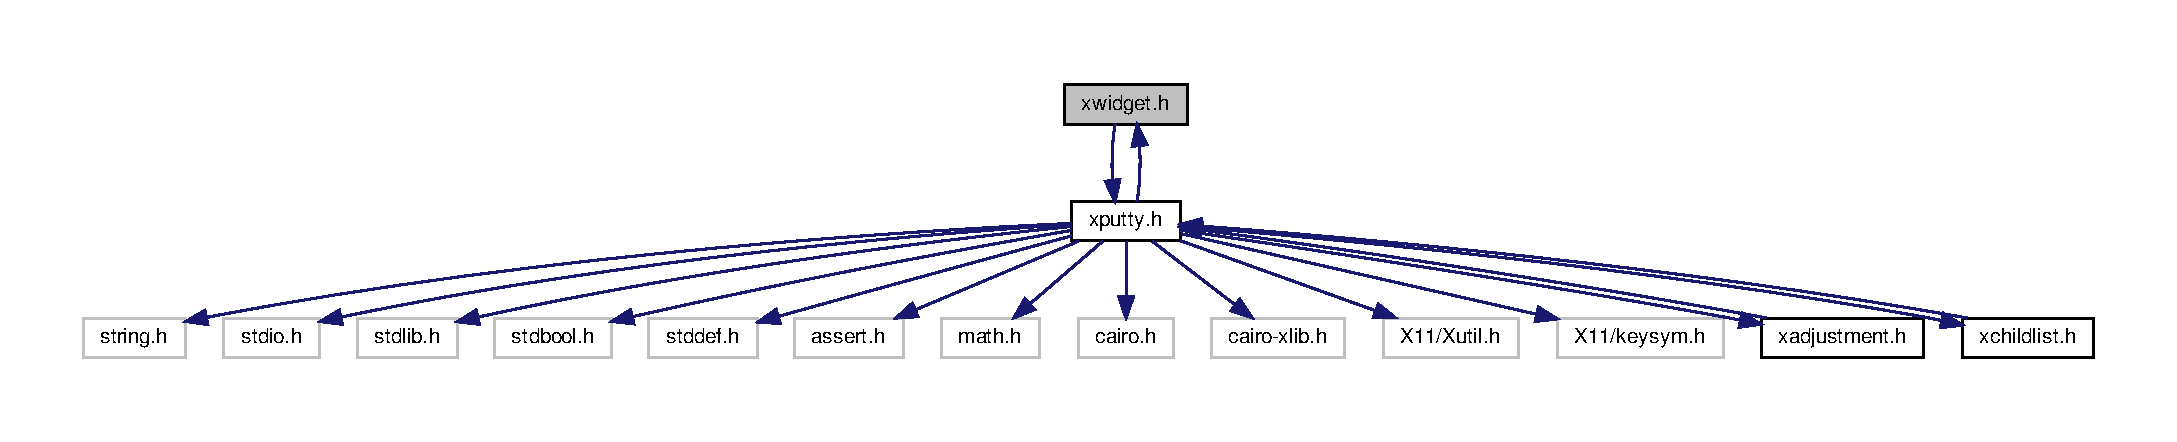
\includegraphics[width=350pt]{xwidget_8h__incl}
\end{center}
\end{figure}
This graph shows which files directly or indirectly include this file\+:
\nopagebreak
\begin{figure}[H]
\begin{center}
\leavevmode
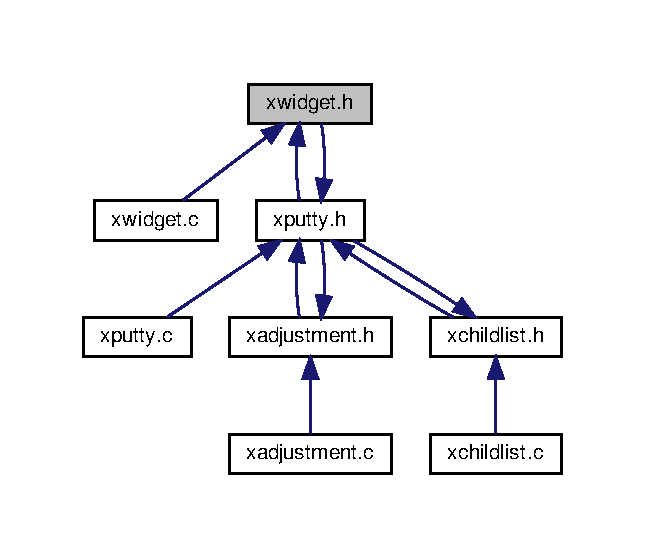
\includegraphics[width=310pt]{xwidget_8h__dep__incl}
\end{center}
\end{figure}
\subsection*{Data Structures}
\begin{DoxyCompactItemize}
\item 
struct \hyperlink{structFunc__t}{Func\+\_\+t}
\begin{DoxyCompactList}\small\item\em \hyperlink{structFunc__t}{Func\+\_\+t} -\/ struct to hold all supported event callbacks. \end{DoxyCompactList}\item 
struct \hyperlink{structResize__t}{Resize\+\_\+t}
\begin{DoxyCompactList}\small\item\em \hyperlink{structResize__t}{Resize\+\_\+t} -\/ struct used to resize child widgets. \end{DoxyCompactList}\item 
struct \hyperlink{structWidget__t}{Widget\+\_\+t}
\begin{DoxyCompactList}\small\item\em \hyperlink{structWidget__t}{Widget\+\_\+t} -\/ struct to hold the basic widget info. \end{DoxyCompactList}\end{DoxyCompactItemize}
\subsection*{Macros}
\begin{DoxyCompactItemize}
\item 
\#define \hyperlink{xwidget_8h_ad56f2f46f2704941329069a12a1a0335}{X\+W\+I\+D\+G\+E\+T\+\_\+H}
\end{DoxyCompactItemize}
\subsection*{Typedefs}
\begin{DoxyCompactItemize}
\item 
typedef void($\ast$ \hyperlink{xwidget_8h_ab4ae973f86a383c8c0f92b709044520a}{evfunc}) (void $\ast$widget, void $\ast$event, void $\ast$user\+\_\+data)
\begin{DoxyCompactList}\small\item\em $\ast$evfunc -\/ function pointer to connect Xevents from the widgets \end{DoxyCompactList}\item 
typedef void($\ast$ \hyperlink{xwidget_8h_a9ef0263424a7f5f8f6b02055fca67ddd}{xevfunc}) (void $\ast$widget, void $\ast$user\+\_\+data)
\begin{DoxyCompactList}\small\item\em $\ast$xevfunc -\/ function pointer to connect X\+Events from the widgets \end{DoxyCompactList}\end{DoxyCompactItemize}
\subsection*{Enumerations}
\begin{DoxyCompactItemize}
\item 
enum \hyperlink{xwidget_8h_a5b77df25933eae1169c9efbc78391ade}{Gravity} \{ \newline
\hyperlink{xwidget_8h_a5b77df25933eae1169c9efbc78391adeac8aee466c121a3c3c942f58e1d8864d4}{N\+O\+R\+T\+H\+W\+E\+ST} = 0x0001, 
\hyperlink{xwidget_8h_a5b77df25933eae1169c9efbc78391adeaa6671505783298e4cb967931c1c1ac5b}{N\+O\+R\+T\+H\+E\+A\+ST} = 0x0002, 
\hyperlink{xwidget_8h_a5b77df25933eae1169c9efbc78391adea6aa90951b336be999de204e61dd366d4}{S\+O\+U\+T\+H\+W\+E\+ST} = 0x0004, 
\hyperlink{xwidget_8h_a5b77df25933eae1169c9efbc78391adea16c2c7abfbd3bad3343b0dcaa858bb49}{S\+O\+U\+T\+H\+E\+A\+ST} = 0x0008, 
\newline
\hyperlink{xwidget_8h_a5b77df25933eae1169c9efbc78391adea2159ffbd3a68037511ab5ab4dd35ace7}{C\+E\+N\+T\+ER} = 0x0016, 
\hyperlink{xwidget_8h_a5b77df25933eae1169c9efbc78391adea8c0a044902c54374c3761b1e06152a1f}{A\+S\+P\+E\+CT} = 0x0032, 
\hyperlink{xwidget_8h_a5b77df25933eae1169c9efbc78391adeac157bdf0b85a40d2619cbc8bc1ae5fe2}{N\+O\+NE} = 0x10000
 \}\begin{DoxyCompactList}\small\item\em Gravity -\/ enum to indicate how to resize a widget. \end{DoxyCompactList}
\end{DoxyCompactItemize}
\subsection*{Functions}
\begin{DoxyCompactItemize}
\item 
\hyperlink{structWidget__t}{Widget\+\_\+t} $\ast$ \hyperlink{xwidget_8h_a5528f841e6b5f2ef62b3b10bfa8bf20f}{create\+\_\+window} (\hyperlink{structXputty}{Xputty} $\ast$app, Window win, int x, int y, int width, int height)
\begin{DoxyCompactList}\small\item\em $\ast$create\+\_\+window -\/ create a Window \end{DoxyCompactList}\item 
\hyperlink{structWidget__t}{Widget\+\_\+t} $\ast$ \hyperlink{xwidget_8h_a2376b5590243f7f4cfd51168af697227}{create\+\_\+widget} (\hyperlink{structXputty}{Xputty} $\ast$app, \hyperlink{structWidget__t}{Widget\+\_\+t} $\ast$win, int x, int y, int width, int height)
\begin{DoxyCompactList}\small\item\em $\ast$create\+\_\+widget -\/ create a widget \end{DoxyCompactList}\item 
void \hyperlink{xwidget_8h_a4d835af5b56eb13ed7bd4602ce7ccd92}{quit} (\hyperlink{structWidget__t}{Widget\+\_\+t} $\ast$w)
\begin{DoxyCompactList}\small\item\em quit -\/ exit the main loop \end{DoxyCompactList}\item 
void \hyperlink{xwidget_8h_ab45a54d3dee60783a5afe9c236f54a04}{transparent\+\_\+draw} (void $\ast$wid, void $\ast$user\+\_\+data)
\begin{DoxyCompactList}\small\item\em \+\_\+transparency -\/ copy parent surface to child surface \end{DoxyCompactList}\item 
void \hyperlink{xwidget_8h_a540b0eefd6f19f487aa71d4c1798ac8c}{destroy\+\_\+widget} (\hyperlink{structWidget__t}{Widget\+\_\+t} $\ast$w, X\+Context Context)
\begin{DoxyCompactList}\small\item\em destroy\+\_\+widget -\/ destroy a widget and remove it from the Context \end{DoxyCompactList}\item 
void \hyperlink{xwidget_8h_af3ecce0332b5f13b590d024db28aec5a}{widget\+\_\+event\+\_\+loop} (void $\ast$w\+\_\+, void $\ast$event, void $\ast$user\+\_\+data)
\begin{DoxyCompactList}\small\item\em widget\+\_\+event\+\_\+loop -\/ the internal widget event loop \end{DoxyCompactList}\item 
void \hyperlink{xwidget_8h_a17f2f3effd46532c596511abcfb5058e}{expose\+\_\+widget} (\hyperlink{structWidget__t}{Widget\+\_\+t} $\ast$w)
\begin{DoxyCompactList}\small\item\em expose\+\_\+widgets -\/ send expose expose event to window \end{DoxyCompactList}\item 
int \hyperlink{xwidget_8h_a1607cf4a642a38ea235a007ea9579403}{key\+\_\+mapping} (Display $\ast$dpy, X\+Key\+Event $\ast$xkey)
\begin{DoxyCompactList}\small\item\em key\+\_\+mapping -\/ modifier key\textquotesingle{}s mapped to a integer value \end{DoxyCompactList}\end{DoxyCompactItemize}


\subsection{Macro Definition Documentation}
\mbox{\Hypertarget{xwidget_8h_ad56f2f46f2704941329069a12a1a0335}\label{xwidget_8h_ad56f2f46f2704941329069a12a1a0335}} 
\index{xwidget.\+h@{xwidget.\+h}!X\+W\+I\+D\+G\+E\+T\+\_\+H@{X\+W\+I\+D\+G\+E\+T\+\_\+H}}
\index{X\+W\+I\+D\+G\+E\+T\+\_\+H@{X\+W\+I\+D\+G\+E\+T\+\_\+H}!xwidget.\+h@{xwidget.\+h}}
\subsubsection{\texorpdfstring{X\+W\+I\+D\+G\+E\+T\+\_\+H}{XWIDGET\_H}}
{\footnotesize\ttfamily \#define X\+W\+I\+D\+G\+E\+T\+\_\+H}



\subsection{Typedef Documentation}
\mbox{\Hypertarget{xwidget_8h_ab4ae973f86a383c8c0f92b709044520a}\label{xwidget_8h_ab4ae973f86a383c8c0f92b709044520a}} 
\index{xwidget.\+h@{xwidget.\+h}!evfunc@{evfunc}}
\index{evfunc@{evfunc}!xwidget.\+h@{xwidget.\+h}}
\subsubsection{\texorpdfstring{evfunc}{evfunc}}
{\footnotesize\ttfamily typedef void($\ast$ evfunc) (void $\ast$widget, void $\ast$event, void $\ast$user\+\_\+data)}



$\ast$evfunc -\/ function pointer to connect Xevents from the widgets 


\begin{DoxyParams}{Parameters}
{\em $\ast$widget} & -\/ void pointer to the widget \\
\hline
{\em $\ast$event} & -\/ void pointer to the X\+Event \\
\hline
{\em $\ast$user\+\_\+data} & -\/ void pointer to attached user\+\_\+data \\
\hline
\end{DoxyParams}
\begin{DoxyReturn}{Returns}
void 
\end{DoxyReturn}
\mbox{\Hypertarget{xwidget_8h_a9ef0263424a7f5f8f6b02055fca67ddd}\label{xwidget_8h_a9ef0263424a7f5f8f6b02055fca67ddd}} 
\index{xwidget.\+h@{xwidget.\+h}!xevfunc@{xevfunc}}
\index{xevfunc@{xevfunc}!xwidget.\+h@{xwidget.\+h}}
\subsubsection{\texorpdfstring{xevfunc}{xevfunc}}
{\footnotesize\ttfamily typedef void($\ast$ xevfunc) (void $\ast$widget, void $\ast$user\+\_\+data)}



$\ast$xevfunc -\/ function pointer to connect X\+Events from the widgets 


\begin{DoxyParams}{Parameters}
{\em $\ast$widget} & -\/ void pointer to the widget \\
\hline
{\em $\ast$user\+\_\+data} & -\/ void pointer to attached user\+\_\+data \\
\hline
\end{DoxyParams}
\begin{DoxyReturn}{Returns}
void 
\end{DoxyReturn}


\subsection{Enumeration Type Documentation}
\mbox{\Hypertarget{xwidget_8h_a5b77df25933eae1169c9efbc78391ade}\label{xwidget_8h_a5b77df25933eae1169c9efbc78391ade}} 
\index{xwidget.\+h@{xwidget.\+h}!Gravity@{Gravity}}
\index{Gravity@{Gravity}!xwidget.\+h@{xwidget.\+h}}
\subsubsection{\texorpdfstring{Gravity}{Gravity}}
{\footnotesize\ttfamily enum \hyperlink{xwidget_8h_a5b77df25933eae1169c9efbc78391ade}{Gravity}}



Gravity -\/ enum to indicate how to resize a widget. 


\begin{DoxyParams}{Parameters}
{\em N\+O\+R\+T\+H\+W\+E\+ST} & -\/ \hyperlink{structWidget__t}{Widget\+\_\+t} adjust nord/west \\
\hline
{\em N\+O\+R\+T\+H\+E\+A\+ST} & -\/ \hyperlink{structWidget__t}{Widget\+\_\+t} adjust nord/east \\
\hline
{\em S\+O\+U\+T\+H\+W\+E\+ST} & -\/ \hyperlink{structWidget__t}{Widget\+\_\+t} adjust south/west \\
\hline
{\em S\+O\+U\+T\+H\+E\+A\+ST} & -\/ \hyperlink{structWidget__t}{Widget\+\_\+t} adjust south/east \\
\hline
{\em C\+E\+N\+T\+ER} & -\/ \hyperlink{structWidget__t}{Widget\+\_\+t} adjust centered \\
\hline
{\em A\+S\+P\+E\+CT} & -\/ \hyperlink{structWidget__t}{Widget\+\_\+t} adjust in a aspect frame \\
\hline
{\em N\+O\+NE} & -\/ \hyperlink{structWidget__t}{Widget\+\_\+t} request no adjustment in frame \\
\hline
\end{DoxyParams}
\begin{DoxyEnumFields}{Enumerator}
\raisebox{\heightof{T}}[0pt][0pt]{\index{N\+O\+R\+T\+H\+W\+E\+ST@{N\+O\+R\+T\+H\+W\+E\+ST}!xwidget.\+h@{xwidget.\+h}}\index{xwidget.\+h@{xwidget.\+h}!N\+O\+R\+T\+H\+W\+E\+ST@{N\+O\+R\+T\+H\+W\+E\+ST}}}\mbox{\Hypertarget{xwidget_8h_a5b77df25933eae1169c9efbc78391adeac8aee466c121a3c3c942f58e1d8864d4}\label{xwidget_8h_a5b77df25933eae1169c9efbc78391adeac8aee466c121a3c3c942f58e1d8864d4}} 
N\+O\+R\+T\+H\+W\+E\+ST&\hyperlink{structWidget__t}{Widget\+\_\+t} adjust nord/west \\
\hline

\raisebox{\heightof{T}}[0pt][0pt]{\index{N\+O\+R\+T\+H\+E\+A\+ST@{N\+O\+R\+T\+H\+E\+A\+ST}!xwidget.\+h@{xwidget.\+h}}\index{xwidget.\+h@{xwidget.\+h}!N\+O\+R\+T\+H\+E\+A\+ST@{N\+O\+R\+T\+H\+E\+A\+ST}}}\mbox{\Hypertarget{xwidget_8h_a5b77df25933eae1169c9efbc78391adeaa6671505783298e4cb967931c1c1ac5b}\label{xwidget_8h_a5b77df25933eae1169c9efbc78391adeaa6671505783298e4cb967931c1c1ac5b}} 
N\+O\+R\+T\+H\+E\+A\+ST&\hyperlink{structWidget__t}{Widget\+\_\+t} adjust nord/east \\
\hline

\raisebox{\heightof{T}}[0pt][0pt]{\index{S\+O\+U\+T\+H\+W\+E\+ST@{S\+O\+U\+T\+H\+W\+E\+ST}!xwidget.\+h@{xwidget.\+h}}\index{xwidget.\+h@{xwidget.\+h}!S\+O\+U\+T\+H\+W\+E\+ST@{S\+O\+U\+T\+H\+W\+E\+ST}}}\mbox{\Hypertarget{xwidget_8h_a5b77df25933eae1169c9efbc78391adea6aa90951b336be999de204e61dd366d4}\label{xwidget_8h_a5b77df25933eae1169c9efbc78391adea6aa90951b336be999de204e61dd366d4}} 
S\+O\+U\+T\+H\+W\+E\+ST&\hyperlink{structWidget__t}{Widget\+\_\+t} adjust south/west \\
\hline

\raisebox{\heightof{T}}[0pt][0pt]{\index{S\+O\+U\+T\+H\+E\+A\+ST@{S\+O\+U\+T\+H\+E\+A\+ST}!xwidget.\+h@{xwidget.\+h}}\index{xwidget.\+h@{xwidget.\+h}!S\+O\+U\+T\+H\+E\+A\+ST@{S\+O\+U\+T\+H\+E\+A\+ST}}}\mbox{\Hypertarget{xwidget_8h_a5b77df25933eae1169c9efbc78391adea16c2c7abfbd3bad3343b0dcaa858bb49}\label{xwidget_8h_a5b77df25933eae1169c9efbc78391adea16c2c7abfbd3bad3343b0dcaa858bb49}} 
S\+O\+U\+T\+H\+E\+A\+ST&\hyperlink{structWidget__t}{Widget\+\_\+t} adjust south/east \\
\hline

\raisebox{\heightof{T}}[0pt][0pt]{\index{C\+E\+N\+T\+ER@{C\+E\+N\+T\+ER}!xwidget.\+h@{xwidget.\+h}}\index{xwidget.\+h@{xwidget.\+h}!C\+E\+N\+T\+ER@{C\+E\+N\+T\+ER}}}\mbox{\Hypertarget{xwidget_8h_a5b77df25933eae1169c9efbc78391adea2159ffbd3a68037511ab5ab4dd35ace7}\label{xwidget_8h_a5b77df25933eae1169c9efbc78391adea2159ffbd3a68037511ab5ab4dd35ace7}} 
C\+E\+N\+T\+ER&\hyperlink{structWidget__t}{Widget\+\_\+t} adjust centered \\
\hline

\raisebox{\heightof{T}}[0pt][0pt]{\index{A\+S\+P\+E\+CT@{A\+S\+P\+E\+CT}!xwidget.\+h@{xwidget.\+h}}\index{xwidget.\+h@{xwidget.\+h}!A\+S\+P\+E\+CT@{A\+S\+P\+E\+CT}}}\mbox{\Hypertarget{xwidget_8h_a5b77df25933eae1169c9efbc78391adea8c0a044902c54374c3761b1e06152a1f}\label{xwidget_8h_a5b77df25933eae1169c9efbc78391adea8c0a044902c54374c3761b1e06152a1f}} 
A\+S\+P\+E\+CT&\hyperlink{structWidget__t}{Widget\+\_\+t} adjust in a aspect frame \\
\hline

\raisebox{\heightof{T}}[0pt][0pt]{\index{N\+O\+NE@{N\+O\+NE}!xwidget.\+h@{xwidget.\+h}}\index{xwidget.\+h@{xwidget.\+h}!N\+O\+NE@{N\+O\+NE}}}\mbox{\Hypertarget{xwidget_8h_a5b77df25933eae1169c9efbc78391adeac157bdf0b85a40d2619cbc8bc1ae5fe2}\label{xwidget_8h_a5b77df25933eae1169c9efbc78391adeac157bdf0b85a40d2619cbc8bc1ae5fe2}} 
N\+O\+NE&\hyperlink{structWidget__t}{Widget\+\_\+t} request no adjustment in frame \\
\hline

\end{DoxyEnumFields}


\subsection{Function Documentation}
\mbox{\Hypertarget{xwidget_8h_a2376b5590243f7f4cfd51168af697227}\label{xwidget_8h_a2376b5590243f7f4cfd51168af697227}} 
\index{xwidget.\+h@{xwidget.\+h}!create\+\_\+widget@{create\+\_\+widget}}
\index{create\+\_\+widget@{create\+\_\+widget}!xwidget.\+h@{xwidget.\+h}}
\subsubsection{\texorpdfstring{create\+\_\+widget()}{create\_widget()}}
{\footnotesize\ttfamily \hyperlink{structWidget__t}{Widget\+\_\+t}$\ast$ create\+\_\+widget (\begin{DoxyParamCaption}\item[{\hyperlink{structXputty}{Xputty} $\ast$}]{app,  }\item[{\hyperlink{structWidget__t}{Widget\+\_\+t} $\ast$}]{parent,  }\item[{int}]{x,  }\item[{int}]{y,  }\item[{int}]{width,  }\item[{int}]{height }\end{DoxyParamCaption})}



$\ast$create\+\_\+widget -\/ create a widget 


\begin{DoxyParams}{Parameters}
{\em $\ast$dpy} & -\/ pointer to the Display to use \\
\hline
{\em $\ast$parent} & -\/ pointer to the Parrent \hyperlink{structWidget__t}{Widget\+\_\+t} \\
\hline
{\em Context} & -\/ a X\+Context to store Window informations \\
\hline
{\em x,y,width,height} & -\/ the position/geometry to create the widget \\
\hline
\end{DoxyParams}
\begin{DoxyReturn}{Returns}
Widget\+\_\+t$\ast$ -\/ pointer to the \hyperlink{structWidget__t}{Widget\+\_\+t} struct 
\end{DoxyReturn}
\mbox{\Hypertarget{xwidget_8h_a5528f841e6b5f2ef62b3b10bfa8bf20f}\label{xwidget_8h_a5528f841e6b5f2ef62b3b10bfa8bf20f}} 
\index{xwidget.\+h@{xwidget.\+h}!create\+\_\+window@{create\+\_\+window}}
\index{create\+\_\+window@{create\+\_\+window}!xwidget.\+h@{xwidget.\+h}}
\subsubsection{\texorpdfstring{create\+\_\+window()}{create\_window()}}
{\footnotesize\ttfamily \hyperlink{structWidget__t}{Widget\+\_\+t}$\ast$ create\+\_\+window (\begin{DoxyParamCaption}\item[{\hyperlink{structXputty}{Xputty} $\ast$}]{app,  }\item[{Window}]{win,  }\item[{int}]{x,  }\item[{int}]{y,  }\item[{int}]{width,  }\item[{int}]{height }\end{DoxyParamCaption})}



$\ast$create\+\_\+window -\/ create a Window 


\begin{DoxyParams}{Parameters}
{\em $\ast$dpy} & -\/ pointer to the Display to use \\
\hline
{\em $\ast$win} & -\/ pointer to the Parrent Window (may be Root) \\
\hline
{\em Context} & -\/ a X\+Context to store Window informations \\
\hline
{\em x,y,width,height} & -\/ the position/geometry to create the window \\
\hline
\end{DoxyParams}
\begin{DoxyReturn}{Returns}
Widget\+\_\+t$\ast$ -\/ pointer to the \hyperlink{structWidget__t}{Widget\+\_\+t} struct
\end{DoxyReturn}

\begin{DoxyParams}{Parameters}
{\em $\ast$dpy} & -\/ pointer to the Display to use \\
\hline
{\em win} & -\/ pointer to the Parrent Window (may be Root) \\
\hline
{\em Context} & -\/ a X\+Context to store Window informations \\
\hline
{\em x,y,width,height} & -\/ the position/geometry to create the window \\
\hline
\end{DoxyParams}
\begin{DoxyReturn}{Returns}
Widget\+\_\+t$\ast$ -\/ pointer to the \hyperlink{structWidget__t}{Widget\+\_\+t} struct 
\end{DoxyReturn}
\mbox{\Hypertarget{xwidget_8h_a540b0eefd6f19f487aa71d4c1798ac8c}\label{xwidget_8h_a540b0eefd6f19f487aa71d4c1798ac8c}} 
\index{xwidget.\+h@{xwidget.\+h}!destroy\+\_\+widget@{destroy\+\_\+widget}}
\index{destroy\+\_\+widget@{destroy\+\_\+widget}!xwidget.\+h@{xwidget.\+h}}
\subsubsection{\texorpdfstring{destroy\+\_\+widget()}{destroy\_widget()}}
{\footnotesize\ttfamily void destroy\+\_\+widget (\begin{DoxyParamCaption}\item[{\hyperlink{structWidget__t}{Widget\+\_\+t} $\ast$}]{w,  }\item[{X\+Context}]{Context }\end{DoxyParamCaption})}



destroy\+\_\+widget -\/ destroy a widget and remove it from the Context 


\begin{DoxyParams}{Parameters}
{\em $\ast$w} & -\/ pointer to the \hyperlink{structWidget__t}{Widget\+\_\+t} sending the request \\
\hline
{\em Context} & -\/ the Context holding the widget info \\
\hline
\end{DoxyParams}
\begin{DoxyReturn}{Returns}
void 
\end{DoxyReturn}
\mbox{\Hypertarget{xwidget_8h_a17f2f3effd46532c596511abcfb5058e}\label{xwidget_8h_a17f2f3effd46532c596511abcfb5058e}} 
\index{xwidget.\+h@{xwidget.\+h}!expose\+\_\+widget@{expose\+\_\+widget}}
\index{expose\+\_\+widget@{expose\+\_\+widget}!xwidget.\+h@{xwidget.\+h}}
\subsubsection{\texorpdfstring{expose\+\_\+widget()}{expose\_widget()}}
{\footnotesize\ttfamily void expose\+\_\+widget (\begin{DoxyParamCaption}\item[{\hyperlink{structWidget__t}{Widget\+\_\+t} $\ast$}]{w }\end{DoxyParamCaption})}



expose\+\_\+widgets -\/ send expose expose event to window 


\begin{DoxyParams}{Parameters}
{\em w} & -\/ the \hyperlink{structWidget__t}{Widget\+\_\+t} to send the event to \\
\hline
\end{DoxyParams}
\begin{DoxyReturn}{Returns}
void 
\end{DoxyReturn}
\mbox{\Hypertarget{xwidget_8h_a1607cf4a642a38ea235a007ea9579403}\label{xwidget_8h_a1607cf4a642a38ea235a007ea9579403}} 
\index{xwidget.\+h@{xwidget.\+h}!key\+\_\+mapping@{key\+\_\+mapping}}
\index{key\+\_\+mapping@{key\+\_\+mapping}!xwidget.\+h@{xwidget.\+h}}
\subsubsection{\texorpdfstring{key\+\_\+mapping()}{key\_mapping()}}
{\footnotesize\ttfamily int key\+\_\+mapping (\begin{DoxyParamCaption}\item[{Display $\ast$}]{dpy,  }\item[{X\+Key\+Event $\ast$}]{xkey }\end{DoxyParamCaption})}



key\+\_\+mapping -\/ modifier key\textquotesingle{}s mapped to a integer value 


\begin{DoxyParams}{Parameters}
{\em $\ast$dpy} & -\/ pointer to the Display in use \\
\hline
{\em $\ast$xkey} & -\/ the key to map \\
\hline
\end{DoxyParams}
\begin{DoxyReturn}{Returns}
int -\/ value (1-\/10) or 0 when not mapped 
\end{DoxyReturn}
\mbox{\Hypertarget{xwidget_8h_a4d835af5b56eb13ed7bd4602ce7ccd92}\label{xwidget_8h_a4d835af5b56eb13ed7bd4602ce7ccd92}} 
\index{xwidget.\+h@{xwidget.\+h}!quit@{quit}}
\index{quit@{quit}!xwidget.\+h@{xwidget.\+h}}
\subsubsection{\texorpdfstring{quit()}{quit()}}
{\footnotesize\ttfamily void quit (\begin{DoxyParamCaption}\item[{\hyperlink{structWidget__t}{Widget\+\_\+t} $\ast$}]{w }\end{DoxyParamCaption})}



quit -\/ exit the main loop 


\begin{DoxyParams}{Parameters}
{\em $\ast$w} & -\/ pointer to the \hyperlink{structWidget__t}{Widget\+\_\+t} sending the request \\
\hline
\end{DoxyParams}
\begin{DoxyReturn}{Returns}
void 
\end{DoxyReturn}
\mbox{\Hypertarget{xwidget_8h_ab45a54d3dee60783a5afe9c236f54a04}\label{xwidget_8h_ab45a54d3dee60783a5afe9c236f54a04}} 
\index{xwidget.\+h@{xwidget.\+h}!transparent\+\_\+draw@{transparent\+\_\+draw}}
\index{transparent\+\_\+draw@{transparent\+\_\+draw}!xwidget.\+h@{xwidget.\+h}}
\subsubsection{\texorpdfstring{transparent\+\_\+draw()}{transparent\_draw()}}
{\footnotesize\ttfamily void transparent\+\_\+draw (\begin{DoxyParamCaption}\item[{void $\ast$}]{w\+\_\+,  }\item[{void $\ast$}]{user\+\_\+data }\end{DoxyParamCaption})}



\+\_\+transparency -\/ copy parent surface to child surface 


\begin{DoxyParams}{Parameters}
{\em $\ast$wid} & -\/ pointer to the \hyperlink{structWidget__t}{Widget\+\_\+t} receiving a event \\
\hline
{\em $\ast$user\+\_\+data} & -\/ void pointer to attached user\+\_\+data \\
\hline
\end{DoxyParams}
\begin{DoxyReturn}{Returns}
void
\end{DoxyReturn}
\+\_\+transparency -\/ copy parent surface to child surface


\begin{DoxyParams}{Parameters}
{\em $\ast$wid} & -\/ pointer to the \hyperlink{structWidget__t}{Widget\+\_\+t} receiving a event \\
\hline
{\em $\ast$user\+\_\+data} & -\/ void pointer to attached user\+\_\+data \\
\hline
\end{DoxyParams}
\begin{DoxyReturn}{Returns}
void 
\end{DoxyReturn}
\mbox{\Hypertarget{xwidget_8h_af3ecce0332b5f13b590d024db28aec5a}\label{xwidget_8h_af3ecce0332b5f13b590d024db28aec5a}} 
\index{xwidget.\+h@{xwidget.\+h}!widget\+\_\+event\+\_\+loop@{widget\+\_\+event\+\_\+loop}}
\index{widget\+\_\+event\+\_\+loop@{widget\+\_\+event\+\_\+loop}!xwidget.\+h@{xwidget.\+h}}
\subsubsection{\texorpdfstring{widget\+\_\+event\+\_\+loop()}{widget\_event\_loop()}}
{\footnotesize\ttfamily void widget\+\_\+event\+\_\+loop (\begin{DoxyParamCaption}\item[{void $\ast$}]{w\+\_\+,  }\item[{void $\ast$}]{event,  }\item[{void $\ast$}]{user\+\_\+data }\end{DoxyParamCaption})}



widget\+\_\+event\+\_\+loop -\/ the internal widget event loop 


\begin{DoxyParams}{Parameters}
{\em $\ast$w} & -\/ pointer to the \hyperlink{structWidget__t}{Widget\+\_\+t} receiving a event \\
\hline
{\em $\ast$event} & -\/ void pointer to the X\+Event \\
\hline
{\em $\ast$user\+\_\+data} & -\/ void pointer to attached user\+\_\+data \\
\hline
\end{DoxyParams}
\begin{DoxyReturn}{Returns}
void 
\end{DoxyReturn}

\hypertarget{xwidget__private_8c}{}\section{xwidget\+\_\+private.\+c File Reference}
\label{xwidget__private_8c}\index{xwidget\+\_\+private.\+c@{xwidget\+\_\+private.\+c}}
{\ttfamily \#include \char`\"{}xwidget\+\_\+private.\+h\char`\"{}}\newline
Include dependency graph for xwidget\+\_\+private.\+c\+:
\nopagebreak
\begin{figure}[H]
\begin{center}
\leavevmode
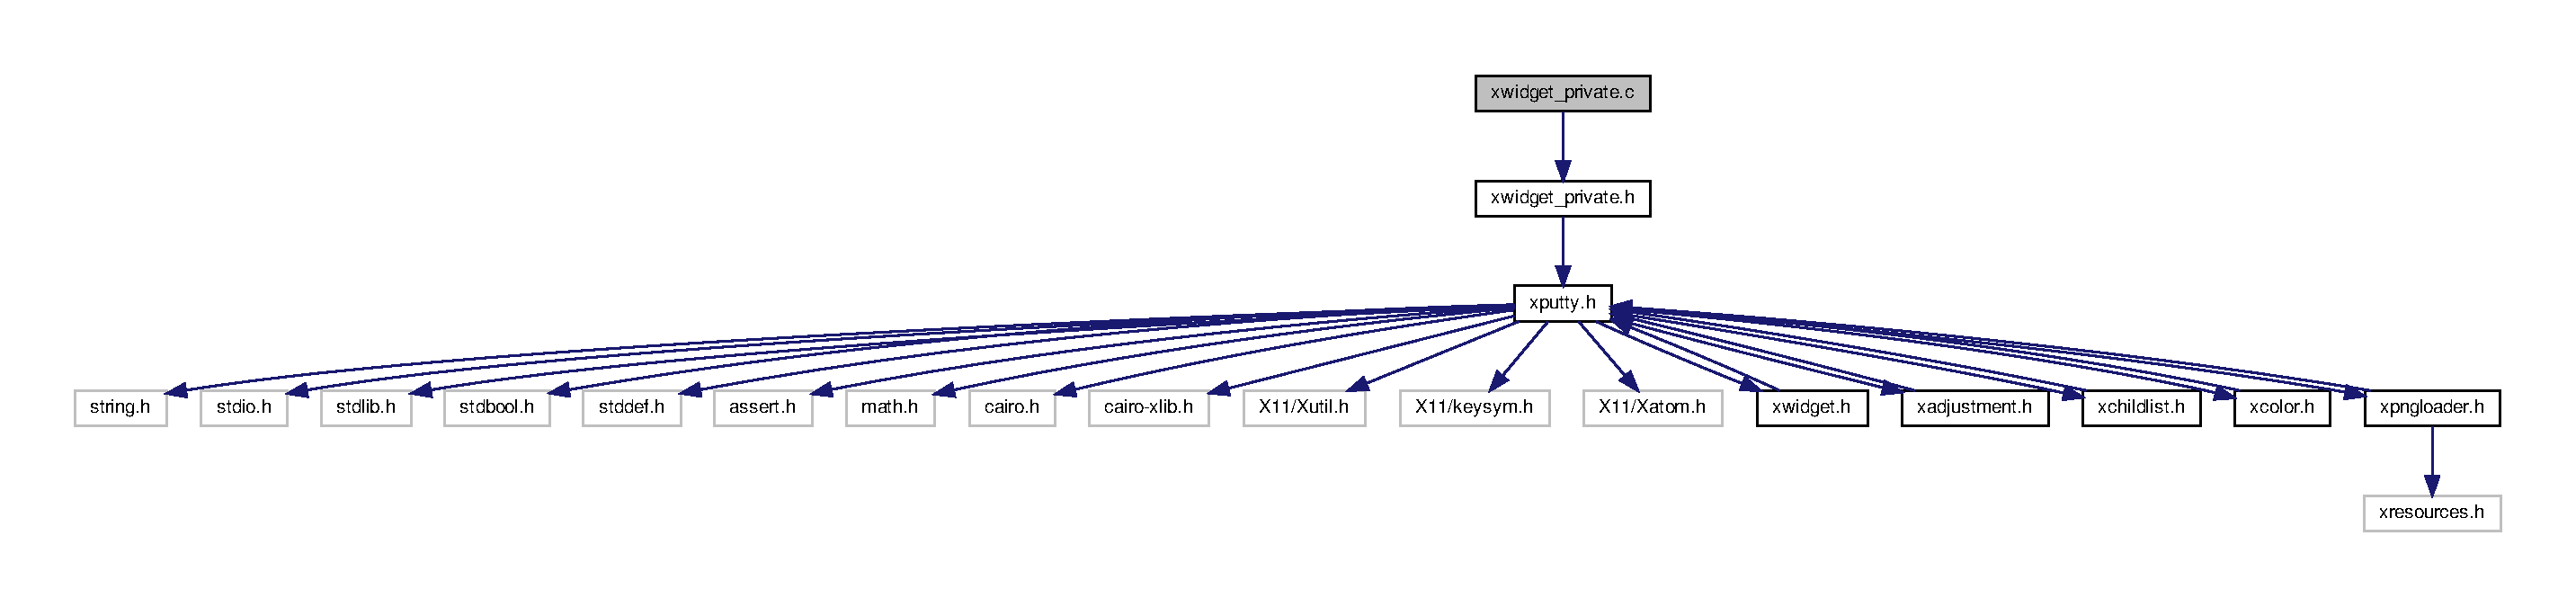
\includegraphics[width=350pt]{xwidget__private_8c__incl}
\end{center}
\end{figure}
\subsection*{Functions}
\begin{DoxyCompactItemize}
\item 
void \hyperlink{xwidget__private_8c_a26c822f013ec5d3d606d0e9648bf1634}{\+\_\+scroll\+\_\+event} (\hyperlink{structWidget__t}{Widget\+\_\+t} $\ast$wid, int direction)
\begin{DoxyCompactList}\small\item\em \+\_\+scroll\+\_\+event -\/ internal check which adjustment needs update \end{DoxyCompactList}\item 
void \hyperlink{xwidget__private_8c_a281115cc04cefd9ff84d2a169515ef69}{\+\_\+toggle\+\_\+event} (\hyperlink{structWidget__t}{Widget\+\_\+t} $\ast$wid)
\begin{DoxyCompactList}\small\item\em \+\_\+toggle\+\_\+event -\/ internal check which adjustment needs update \end{DoxyCompactList}\item 
void \hyperlink{xwidget__private_8c_a3fa824e7c223fab91f65dbdcd3e07f18}{\+\_\+check\+\_\+enum} (\hyperlink{structWidget__t}{Widget\+\_\+t} $\ast$wid, X\+Button\+Event $\ast$xbutton)
\begin{DoxyCompactList}\small\item\em \+\_\+check\+\_\+enum -\/ internal check which adjustment needs update \end{DoxyCompactList}\item 
void \hyperlink{xwidget__private_8c_a58ae554632b1c9f7afc73aa159a1dc0c}{\+\_\+button\+\_\+press} (\hyperlink{structWidget__t}{Widget\+\_\+t} $\ast$wid, X\+Button\+Event $\ast$xbutton, void $\ast$user\+\_\+data)
\begin{DoxyCompactList}\small\item\em \+\_\+button\+\_\+press -\/ internal check which button is pressed \end{DoxyCompactList}\item 
void \hyperlink{xwidget__private_8c_a4268fe28baeb0a66234a976f14c6975b}{\+\_\+check\+\_\+grab} (\hyperlink{structWidget__t}{Widget\+\_\+t} $\ast$wid, X\+Button\+Event $\ast$xbutton, \hyperlink{structXputty}{Xputty} $\ast$main)
\begin{DoxyCompactList}\small\item\em \+\_\+check\+\_\+grab -\/ internal check if menu is pressed \end{DoxyCompactList}\item 
void \hyperlink{xwidget__private_8c_aaaac44f0d2bcf2ddc3f76b79e74fb3b6}{\+\_\+propagate\+\_\+child\+\_\+expose} (\hyperlink{structWidget__t}{Widget\+\_\+t} $\ast$wid)
\begin{DoxyCompactList}\small\item\em \+\_\+propagate\+\_\+childs -\/ send expose to child window \end{DoxyCompactList}\item 
void \hyperlink{xwidget__private_8c_ae2aeefa7b35ff7e10a148e8438a12dc9}{\+\_\+check\+\_\+keymap} (void $\ast$w\+\_\+, X\+Key\+Event xkey)
\begin{DoxyCompactList}\small\item\em \+\_\+check\+\_\+keymap -\/ check if key is in map, send requests if so \end{DoxyCompactList}\item 
void \hyperlink{xwidget__private_8c_ae8d8e0d87f6186d3d19f1372c357edbe}{\+\_\+has\+\_\+pointer} (\hyperlink{structWidget__t}{Widget\+\_\+t} $\ast$w, X\+Button\+Event $\ast$button)
\begin{DoxyCompactList}\small\item\em \+\_\+has\+\_\+pointer -\/ check if the widget has the pointer on Button release \end{DoxyCompactList}\item 
void \hyperlink{xwidget__private_8c_a227521763a2c42146302b62c79e97ac2}{\+\_\+set\+\_\+adj\+\_\+value} (void $\ast$w\+\_\+, bool x, int direction)
\begin{DoxyCompactList}\small\item\em \+\_\+set\+\_\+adj\+\_\+value -\/ set value to adjustment from key event \end{DoxyCompactList}\item 
void \hyperlink{xwidget__private_8c_ac337b3d0f61bc649c955c6e5bf14c810}{\+\_\+dummy1\+\_\+callback} (void $\ast$w\+\_\+, void $\ast$\+\_\+data, void $\ast$user\+\_\+data)
\begin{DoxyCompactList}\small\item\em \+\_\+dummy1\+\_\+callback -\/ default debuging callback for evfunc\textquotesingle{}s \end{DoxyCompactList}\item 
void \hyperlink{xwidget__private_8c_a70d121b920c02065b3bc096c9b92e83c}{\+\_\+dummy\+\_\+callback} (void $\ast$w\+\_\+, void $\ast$user\+\_\+data)
\begin{DoxyCompactList}\small\item\em \+\_\+dummy1\+\_\+callback -\/ default debuging callback for xevfunc\textquotesingle{}s \end{DoxyCompactList}\item 
void \hyperlink{xwidget__private_8c_a114b183c93f55d46f7071c9ef6110b02}{\+\_\+resize\+\_\+surface} (\hyperlink{structWidget__t}{Widget\+\_\+t} $\ast$wid, int width, int height)
\begin{DoxyCompactList}\small\item\em \+\_\+resize\+\_\+surface -\/ intern check if surfaces needs resizing \end{DoxyCompactList}\item 
void \hyperlink{xwidget__private_8c_a211aa2f671aa4c2885bc05e033eef8c4}{\+\_\+resize\+\_\+childs} (\hyperlink{structWidget__t}{Widget\+\_\+t} $\ast$wid)
\begin{DoxyCompactList}\small\item\em \+\_\+resize\+\_\+childs -\/ intern check if child widgets needs resizing \end{DoxyCompactList}\end{DoxyCompactItemize}


\subsection{Function Documentation}
\mbox{\Hypertarget{xwidget__private_8c_a58ae554632b1c9f7afc73aa159a1dc0c}\label{xwidget__private_8c_a58ae554632b1c9f7afc73aa159a1dc0c}} 
\index{xwidget\+\_\+private.\+c@{xwidget\+\_\+private.\+c}!\+\_\+button\+\_\+press@{\+\_\+button\+\_\+press}}
\index{\+\_\+button\+\_\+press@{\+\_\+button\+\_\+press}!xwidget\+\_\+private.\+c@{xwidget\+\_\+private.\+c}}
\subsubsection{\texorpdfstring{\+\_\+button\+\_\+press()}{\_button\_press()}}
{\footnotesize\ttfamily void \+\_\+button\+\_\+press (\begin{DoxyParamCaption}\item[{\hyperlink{structWidget__t}{Widget\+\_\+t} $\ast$}]{wid,  }\item[{X\+Button\+Event $\ast$}]{xbutton,  }\item[{void $\ast$}]{user\+\_\+data }\end{DoxyParamCaption})}



\+\_\+button\+\_\+press -\/ internal check which button is pressed 


\begin{DoxyParams}{Parameters}
{\em $\ast$wid} & -\/ pointer to the \hyperlink{structWidget__t}{Widget\+\_\+t} receiving a event \\
\hline
{\em $\ast$xbutton} & -\/ pointer to the X\+Button\+Event \\
\hline
{\em $\ast$user\+\_\+data} & -\/ void pointer to attached user\+\_\+data \\
\hline
\end{DoxyParams}
\begin{DoxyReturn}{Returns}
void 
\end{DoxyReturn}
\mbox{\Hypertarget{xwidget__private_8c_a3fa824e7c223fab91f65dbdcd3e07f18}\label{xwidget__private_8c_a3fa824e7c223fab91f65dbdcd3e07f18}} 
\index{xwidget\+\_\+private.\+c@{xwidget\+\_\+private.\+c}!\+\_\+check\+\_\+enum@{\+\_\+check\+\_\+enum}}
\index{\+\_\+check\+\_\+enum@{\+\_\+check\+\_\+enum}!xwidget\+\_\+private.\+c@{xwidget\+\_\+private.\+c}}
\subsubsection{\texorpdfstring{\+\_\+check\+\_\+enum()}{\_check\_enum()}}
{\footnotesize\ttfamily void \+\_\+check\+\_\+enum (\begin{DoxyParamCaption}\item[{\hyperlink{structWidget__t}{Widget\+\_\+t} $\ast$}]{wid,  }\item[{X\+Button\+Event $\ast$}]{xbutton }\end{DoxyParamCaption})}



\+\_\+check\+\_\+enum -\/ internal check which adjustment needs update 


\begin{DoxyParams}{Parameters}
{\em $\ast$wid} & -\/ pointer to the \hyperlink{structWidget__t}{Widget\+\_\+t} receiving a event \\
\hline
{\em $\ast$xbutton} & -\/ pointer to the X\+Button\+Event \\
\hline
\end{DoxyParams}
\begin{DoxyReturn}{Returns}
void 
\end{DoxyReturn}
\mbox{\Hypertarget{xwidget__private_8c_a4268fe28baeb0a66234a976f14c6975b}\label{xwidget__private_8c_a4268fe28baeb0a66234a976f14c6975b}} 
\index{xwidget\+\_\+private.\+c@{xwidget\+\_\+private.\+c}!\+\_\+check\+\_\+grab@{\+\_\+check\+\_\+grab}}
\index{\+\_\+check\+\_\+grab@{\+\_\+check\+\_\+grab}!xwidget\+\_\+private.\+c@{xwidget\+\_\+private.\+c}}
\subsubsection{\texorpdfstring{\+\_\+check\+\_\+grab()}{\_check\_grab()}}
{\footnotesize\ttfamily void \+\_\+check\+\_\+grab (\begin{DoxyParamCaption}\item[{\hyperlink{structWidget__t}{Widget\+\_\+t} $\ast$}]{wid,  }\item[{X\+Button\+Event $\ast$}]{xbutton,  }\item[{\hyperlink{structXputty}{Xputty} $\ast$}]{main }\end{DoxyParamCaption})}



\+\_\+check\+\_\+grab -\/ internal check if menu is pressed 


\begin{DoxyParams}{Parameters}
{\em $\ast$wid} & -\/ pointer to the \hyperlink{structWidget__t}{Widget\+\_\+t} receiving a event \\
\hline
{\em $\ast$xbutton} & -\/ pointer to the X\+Button\+Event \\
\hline
{\em $\ast$main} & -\/ pointer to main struct \\
\hline
\end{DoxyParams}
\begin{DoxyReturn}{Returns}
void 
\end{DoxyReturn}
\mbox{\Hypertarget{xwidget__private_8c_ae2aeefa7b35ff7e10a148e8438a12dc9}\label{xwidget__private_8c_ae2aeefa7b35ff7e10a148e8438a12dc9}} 
\index{xwidget\+\_\+private.\+c@{xwidget\+\_\+private.\+c}!\+\_\+check\+\_\+keymap@{\+\_\+check\+\_\+keymap}}
\index{\+\_\+check\+\_\+keymap@{\+\_\+check\+\_\+keymap}!xwidget\+\_\+private.\+c@{xwidget\+\_\+private.\+c}}
\subsubsection{\texorpdfstring{\+\_\+check\+\_\+keymap()}{\_check\_keymap()}}
{\footnotesize\ttfamily void \+\_\+check\+\_\+keymap (\begin{DoxyParamCaption}\item[{void $\ast$}]{w\+\_\+,  }\item[{X\+Key\+Event}]{xkey }\end{DoxyParamCaption})}



\+\_\+check\+\_\+keymap -\/ check if key is in map, send requests if so 


\begin{DoxyParams}{Parameters}
{\em $\ast$w} & -\/ pointer to the \hyperlink{structWidget__t}{Widget\+\_\+t} receiving the event \\
\hline
{\em xkey} & -\/ the X\+Key\+Event to check \\
\hline
\end{DoxyParams}
\begin{DoxyReturn}{Returns}
void 
\end{DoxyReturn}
\mbox{\Hypertarget{xwidget__private_8c_ac337b3d0f61bc649c955c6e5bf14c810}\label{xwidget__private_8c_ac337b3d0f61bc649c955c6e5bf14c810}} 
\index{xwidget\+\_\+private.\+c@{xwidget\+\_\+private.\+c}!\+\_\+dummy1\+\_\+callback@{\+\_\+dummy1\+\_\+callback}}
\index{\+\_\+dummy1\+\_\+callback@{\+\_\+dummy1\+\_\+callback}!xwidget\+\_\+private.\+c@{xwidget\+\_\+private.\+c}}
\subsubsection{\texorpdfstring{\+\_\+dummy1\+\_\+callback()}{\_dummy1\_callback()}}
{\footnotesize\ttfamily void \+\_\+dummy1\+\_\+callback (\begin{DoxyParamCaption}\item[{void $\ast$}]{w\+\_\+,  }\item[{void $\ast$}]{\+\_\+data,  }\item[{void $\ast$}]{user\+\_\+data }\end{DoxyParamCaption})}



\+\_\+dummy1\+\_\+callback -\/ default debuging callback for evfunc\textquotesingle{}s 


\begin{DoxyParams}{Parameters}
{\em $\ast$w} & -\/ pointer to the \hyperlink{structWidget__t}{Widget\+\_\+t} receive the event \\
\hline
{\em user\+\_\+data} & -\/ void pointer to attached user\+\_\+data \\
\hline
\end{DoxyParams}
\begin{DoxyReturn}{Returns}
void 
\end{DoxyReturn}
\mbox{\Hypertarget{xwidget__private_8c_a70d121b920c02065b3bc096c9b92e83c}\label{xwidget__private_8c_a70d121b920c02065b3bc096c9b92e83c}} 
\index{xwidget\+\_\+private.\+c@{xwidget\+\_\+private.\+c}!\+\_\+dummy\+\_\+callback@{\+\_\+dummy\+\_\+callback}}
\index{\+\_\+dummy\+\_\+callback@{\+\_\+dummy\+\_\+callback}!xwidget\+\_\+private.\+c@{xwidget\+\_\+private.\+c}}
\subsubsection{\texorpdfstring{\+\_\+dummy\+\_\+callback()}{\_dummy\_callback()}}
{\footnotesize\ttfamily void \+\_\+dummy\+\_\+callback (\begin{DoxyParamCaption}\item[{void $\ast$}]{w\+\_\+,  }\item[{void $\ast$}]{user\+\_\+data }\end{DoxyParamCaption})}



\+\_\+dummy1\+\_\+callback -\/ default debuging callback for xevfunc\textquotesingle{}s 


\begin{DoxyParams}{Parameters}
{\em $\ast$w} & -\/ pointer to the \hyperlink{structWidget__t}{Widget\+\_\+t} receive the event \\
\hline
{\em user\+\_\+data} & -\/ void pointer to attached user\+\_\+data \\
\hline
\end{DoxyParams}
\begin{DoxyReturn}{Returns}
void 
\end{DoxyReturn}
\mbox{\Hypertarget{xwidget__private_8c_ae8d8e0d87f6186d3d19f1372c357edbe}\label{xwidget__private_8c_ae8d8e0d87f6186d3d19f1372c357edbe}} 
\index{xwidget\+\_\+private.\+c@{xwidget\+\_\+private.\+c}!\+\_\+has\+\_\+pointer@{\+\_\+has\+\_\+pointer}}
\index{\+\_\+has\+\_\+pointer@{\+\_\+has\+\_\+pointer}!xwidget\+\_\+private.\+c@{xwidget\+\_\+private.\+c}}
\subsubsection{\texorpdfstring{\+\_\+has\+\_\+pointer()}{\_has\_pointer()}}
{\footnotesize\ttfamily void \+\_\+has\+\_\+pointer (\begin{DoxyParamCaption}\item[{\hyperlink{structWidget__t}{Widget\+\_\+t} $\ast$}]{w,  }\item[{X\+Button\+Event $\ast$}]{button }\end{DoxyParamCaption})}



\+\_\+has\+\_\+pointer -\/ check if the widget has the pointer on Button release 


\begin{DoxyParams}{Parameters}
{\em $\ast$w} & -\/ pointer to the \hyperlink{structWidget__t}{Widget\+\_\+t} sending the request \\
\hline
{\em $\ast$button} & -\/ pointer to the X\+Button\+Event sending the notify \\
\hline
\end{DoxyParams}
\begin{DoxyReturn}{Returns}
void 
\end{DoxyReturn}
\mbox{\Hypertarget{xwidget__private_8c_aaaac44f0d2bcf2ddc3f76b79e74fb3b6}\label{xwidget__private_8c_aaaac44f0d2bcf2ddc3f76b79e74fb3b6}} 
\index{xwidget\+\_\+private.\+c@{xwidget\+\_\+private.\+c}!\+\_\+propagate\+\_\+child\+\_\+expose@{\+\_\+propagate\+\_\+child\+\_\+expose}}
\index{\+\_\+propagate\+\_\+child\+\_\+expose@{\+\_\+propagate\+\_\+child\+\_\+expose}!xwidget\+\_\+private.\+c@{xwidget\+\_\+private.\+c}}
\subsubsection{\texorpdfstring{\+\_\+propagate\+\_\+child\+\_\+expose()}{\_propagate\_child\_expose()}}
{\footnotesize\ttfamily void \+\_\+propagate\+\_\+child\+\_\+expose (\begin{DoxyParamCaption}\item[{\hyperlink{structWidget__t}{Widget\+\_\+t} $\ast$}]{wid }\end{DoxyParamCaption})}



\+\_\+propagate\+\_\+childs -\/ send expose to child window 


\begin{DoxyParams}{Parameters}
{\em $\ast$wid} & -\/ pointer to the \hyperlink{structWidget__t}{Widget\+\_\+t} send the event \\
\hline
\end{DoxyParams}
\begin{DoxyReturn}{Returns}
void 
\end{DoxyReturn}
\mbox{\Hypertarget{xwidget__private_8c_a211aa2f671aa4c2885bc05e033eef8c4}\label{xwidget__private_8c_a211aa2f671aa4c2885bc05e033eef8c4}} 
\index{xwidget\+\_\+private.\+c@{xwidget\+\_\+private.\+c}!\+\_\+resize\+\_\+childs@{\+\_\+resize\+\_\+childs}}
\index{\+\_\+resize\+\_\+childs@{\+\_\+resize\+\_\+childs}!xwidget\+\_\+private.\+c@{xwidget\+\_\+private.\+c}}
\subsubsection{\texorpdfstring{\+\_\+resize\+\_\+childs()}{\_resize\_childs()}}
{\footnotesize\ttfamily void \+\_\+resize\+\_\+childs (\begin{DoxyParamCaption}\item[{\hyperlink{structWidget__t}{Widget\+\_\+t} $\ast$}]{wid }\end{DoxyParamCaption})}



\+\_\+resize\+\_\+childs -\/ intern check if child widgets needs resizing 


\begin{DoxyParams}{Parameters}
{\em $\ast$wid} & -\/ pointer to the \hyperlink{structWidget__t}{Widget\+\_\+t} receive the event \\
\hline
\end{DoxyParams}
\begin{DoxyReturn}{Returns}
void 
\end{DoxyReturn}
\mbox{\Hypertarget{xwidget__private_8c_a114b183c93f55d46f7071c9ef6110b02}\label{xwidget__private_8c_a114b183c93f55d46f7071c9ef6110b02}} 
\index{xwidget\+\_\+private.\+c@{xwidget\+\_\+private.\+c}!\+\_\+resize\+\_\+surface@{\+\_\+resize\+\_\+surface}}
\index{\+\_\+resize\+\_\+surface@{\+\_\+resize\+\_\+surface}!xwidget\+\_\+private.\+c@{xwidget\+\_\+private.\+c}}
\subsubsection{\texorpdfstring{\+\_\+resize\+\_\+surface()}{\_resize\_surface()}}
{\footnotesize\ttfamily void \+\_\+resize\+\_\+surface (\begin{DoxyParamCaption}\item[{\hyperlink{structWidget__t}{Widget\+\_\+t} $\ast$}]{wid,  }\item[{int}]{width,  }\item[{int}]{height }\end{DoxyParamCaption})}



\+\_\+resize\+\_\+surface -\/ intern check if surfaces needs resizing 


\begin{DoxyParams}{Parameters}
{\em $\ast$wid} & -\/ pointer to the \hyperlink{structWidget__t}{Widget\+\_\+t} receive the event \\
\hline
{\em width} & -\/ the new width \\
\hline
{\em height} & -\/ the new height \\
\hline
\end{DoxyParams}
\begin{DoxyReturn}{Returns}
void 
\end{DoxyReturn}
\mbox{\Hypertarget{xwidget__private_8c_a26c822f013ec5d3d606d0e9648bf1634}\label{xwidget__private_8c_a26c822f013ec5d3d606d0e9648bf1634}} 
\index{xwidget\+\_\+private.\+c@{xwidget\+\_\+private.\+c}!\+\_\+scroll\+\_\+event@{\+\_\+scroll\+\_\+event}}
\index{\+\_\+scroll\+\_\+event@{\+\_\+scroll\+\_\+event}!xwidget\+\_\+private.\+c@{xwidget\+\_\+private.\+c}}
\subsubsection{\texorpdfstring{\+\_\+scroll\+\_\+event()}{\_scroll\_event()}}
{\footnotesize\ttfamily void \+\_\+scroll\+\_\+event (\begin{DoxyParamCaption}\item[{\hyperlink{structWidget__t}{Widget\+\_\+t} $\ast$}]{wid,  }\item[{int}]{direction }\end{DoxyParamCaption})}



\+\_\+scroll\+\_\+event -\/ internal check which adjustment needs update 


\begin{DoxyParams}{Parameters}
{\em $\ast$wid} & -\/ pointer to the \hyperlink{structWidget__t}{Widget\+\_\+t} receiving a event \\
\hline
{\em direction} & -\/ up/down scroll diretion \\
\hline
\end{DoxyParams}
\begin{DoxyReturn}{Returns}
void 
\end{DoxyReturn}
\mbox{\Hypertarget{xwidget__private_8c_a227521763a2c42146302b62c79e97ac2}\label{xwidget__private_8c_a227521763a2c42146302b62c79e97ac2}} 
\index{xwidget\+\_\+private.\+c@{xwidget\+\_\+private.\+c}!\+\_\+set\+\_\+adj\+\_\+value@{\+\_\+set\+\_\+adj\+\_\+value}}
\index{\+\_\+set\+\_\+adj\+\_\+value@{\+\_\+set\+\_\+adj\+\_\+value}!xwidget\+\_\+private.\+c@{xwidget\+\_\+private.\+c}}
\subsubsection{\texorpdfstring{\+\_\+set\+\_\+adj\+\_\+value()}{\_set\_adj\_value()}}
{\footnotesize\ttfamily void \+\_\+set\+\_\+adj\+\_\+value (\begin{DoxyParamCaption}\item[{void $\ast$}]{w\+\_\+,  }\item[{bool}]{x,  }\item[{int}]{direction }\end{DoxyParamCaption})}



\+\_\+set\+\_\+adj\+\_\+value -\/ set value to adjustment from key event 


\begin{DoxyParams}{Parameters}
{\em $\ast$w} & -\/ pointer to the \hyperlink{structWidget__t}{Widget\+\_\+t} receiving the event \\
\hline
{\em x} & -\/ use x or y-\/axis \\
\hline
\end{DoxyParams}
\begin{DoxyReturn}{Returns}
void 
\end{DoxyReturn}
\mbox{\Hypertarget{xwidget__private_8c_a281115cc04cefd9ff84d2a169515ef69}\label{xwidget__private_8c_a281115cc04cefd9ff84d2a169515ef69}} 
\index{xwidget\+\_\+private.\+c@{xwidget\+\_\+private.\+c}!\+\_\+toggle\+\_\+event@{\+\_\+toggle\+\_\+event}}
\index{\+\_\+toggle\+\_\+event@{\+\_\+toggle\+\_\+event}!xwidget\+\_\+private.\+c@{xwidget\+\_\+private.\+c}}
\subsubsection{\texorpdfstring{\+\_\+toggle\+\_\+event()}{\_toggle\_event()}}
{\footnotesize\ttfamily void \+\_\+toggle\+\_\+event (\begin{DoxyParamCaption}\item[{\hyperlink{structWidget__t}{Widget\+\_\+t} $\ast$}]{wid }\end{DoxyParamCaption})}



\+\_\+toggle\+\_\+event -\/ internal check which adjustment needs update 


\begin{DoxyParams}{Parameters}
{\em $\ast$wid} & -\/ pointer to the \hyperlink{structWidget__t}{Widget\+\_\+t} receiving a event \\
\hline
{\em direction} & -\/ up/down scroll diretion \\
\hline
\end{DoxyParams}
\begin{DoxyReturn}{Returns}
void 
\end{DoxyReturn}

\hypertarget{xwidget__private_8h}{}\section{xwidget\+\_\+private.\+h File Reference}
\label{xwidget__private_8h}\index{xwidget\+\_\+private.\+h@{xwidget\+\_\+private.\+h}}
{\ttfamily \#include \char`\"{}xputty.\+h\char`\"{}}\newline
Include dependency graph for xwidget\+\_\+private.\+h\+:
\nopagebreak
\begin{figure}[H]
\begin{center}
\leavevmode
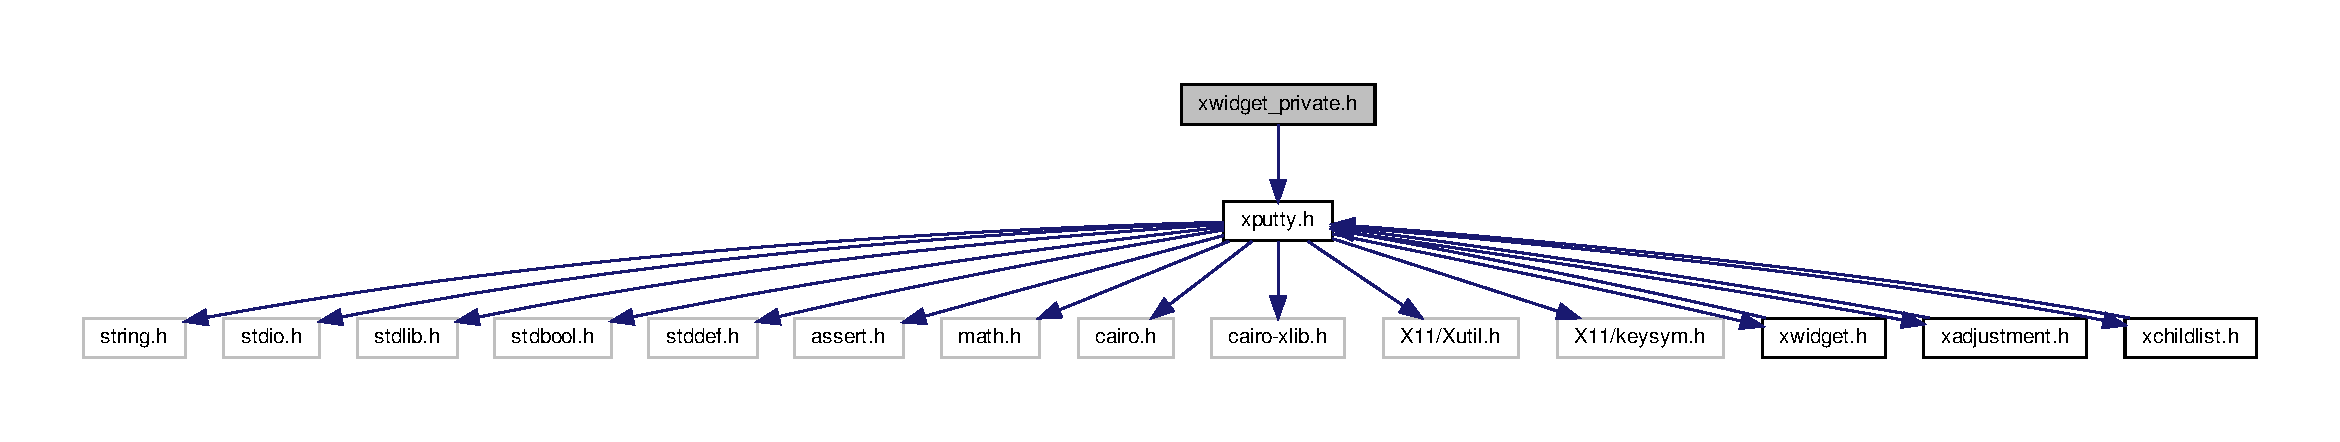
\includegraphics[width=350pt]{xwidget__private_8h__incl}
\end{center}
\end{figure}
This graph shows which files directly or indirectly include this file\+:
\nopagebreak
\begin{figure}[H]
\begin{center}
\leavevmode
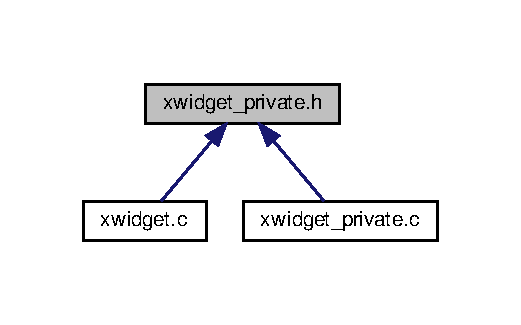
\includegraphics[width=250pt]{xwidget__private_8h__dep__incl}
\end{center}
\end{figure}
\subsection*{Macros}
\begin{DoxyCompactItemize}
\item 
\#define \hyperlink{xwidget__private_8h_ae1930d67bcc5abcf90eec1f62804d841}{X\+W\+I\+D\+G\+E\+T\+\_\+\+P\+R\+I\+V\+A\+T\+E\+\_\+\+H\+\_\+}
\end{DoxyCompactItemize}
\subsection*{Functions}
\begin{DoxyCompactItemize}
\item 
void \hyperlink{xwidget__private_8h_a26c822f013ec5d3d606d0e9648bf1634}{\+\_\+scroll\+\_\+event} (\hyperlink{structWidget__t}{Widget\+\_\+t} $\ast$wid, int direction)
\begin{DoxyCompactList}\small\item\em \+\_\+scroll\+\_\+event -\/ internal check which adjustment needs update \end{DoxyCompactList}\item 
void \hyperlink{xwidget__private_8h_a281115cc04cefd9ff84d2a169515ef69}{\+\_\+toggle\+\_\+event} (\hyperlink{structWidget__t}{Widget\+\_\+t} $\ast$wid)
\begin{DoxyCompactList}\small\item\em \+\_\+toggle\+\_\+event -\/ internal check which adjustment needs update \end{DoxyCompactList}\item 
void \hyperlink{xwidget__private_8h_a3fa824e7c223fab91f65dbdcd3e07f18}{\+\_\+check\+\_\+enum} (\hyperlink{structWidget__t}{Widget\+\_\+t} $\ast$wid, X\+Button\+Event $\ast$xbutton)
\begin{DoxyCompactList}\small\item\em \+\_\+check\+\_\+enum -\/ internal check which adjustment needs update \end{DoxyCompactList}\item 
void \hyperlink{xwidget__private_8h_a58ae554632b1c9f7afc73aa159a1dc0c}{\+\_\+button\+\_\+press} (\hyperlink{structWidget__t}{Widget\+\_\+t} $\ast$wid, X\+Button\+Event $\ast$xbutton, void $\ast$user\+\_\+data)
\begin{DoxyCompactList}\small\item\em \+\_\+button\+\_\+press -\/ internal check which button is pressed \end{DoxyCompactList}\item 
void \hyperlink{xwidget__private_8h_a4268fe28baeb0a66234a976f14c6975b}{\+\_\+check\+\_\+grab} (\hyperlink{structWidget__t}{Widget\+\_\+t} $\ast$wid, X\+Button\+Event $\ast$xbutton, \hyperlink{structXputty}{Xputty} $\ast$main)
\begin{DoxyCompactList}\small\item\em \+\_\+check\+\_\+grab -\/ internal check if menu is pressed \end{DoxyCompactList}\item 
void \hyperlink{xwidget__private_8h_aaaac44f0d2bcf2ddc3f76b79e74fb3b6}{\+\_\+propagate\+\_\+child\+\_\+expose} (\hyperlink{structWidget__t}{Widget\+\_\+t} $\ast$wid)
\begin{DoxyCompactList}\small\item\em \+\_\+propagate\+\_\+childs -\/ send expose to child window \end{DoxyCompactList}\item 
void \hyperlink{xwidget__private_8h_ae2aeefa7b35ff7e10a148e8438a12dc9}{\+\_\+check\+\_\+keymap} (void $\ast$w\+\_\+, X\+Key\+Event xkey)
\begin{DoxyCompactList}\small\item\em \+\_\+check\+\_\+keymap -\/ check if key is in map, send requests if so \end{DoxyCompactList}\item 
void \hyperlink{xwidget__private_8h_a3303d77cae03bc9141355e43fc6fe97f}{\+\_\+hide\+\_\+all\+\_\+tooltips} (\hyperlink{structWidget__t}{Widget\+\_\+t} $\ast$wid)
\begin{DoxyCompactList}\small\item\em \+\_\+hide\+\_\+all\+\_\+tooltips -\/ hide all active tooltips \end{DoxyCompactList}\item 
void \hyperlink{xwidget__private_8h_ae8d8e0d87f6186d3d19f1372c357edbe}{\+\_\+has\+\_\+pointer} (\hyperlink{structWidget__t}{Widget\+\_\+t} $\ast$w, X\+Button\+Event $\ast$button)
\begin{DoxyCompactList}\small\item\em \+\_\+has\+\_\+pointer -\/ check if the widget has the pointer on Button release \end{DoxyCompactList}\item 
void \hyperlink{xwidget__private_8h_a227521763a2c42146302b62c79e97ac2}{\+\_\+set\+\_\+adj\+\_\+value} (void $\ast$w\+\_\+, bool x, int direction)
\begin{DoxyCompactList}\small\item\em \+\_\+set\+\_\+adj\+\_\+value -\/ set value to adjustment from key event \end{DoxyCompactList}\item 
void \hyperlink{xwidget__private_8h_ac337b3d0f61bc649c955c6e5bf14c810}{\+\_\+dummy1\+\_\+callback} (void $\ast$w\+\_\+, void $\ast$\+\_\+data, void $\ast$user\+\_\+data)
\begin{DoxyCompactList}\small\item\em \+\_\+dummy1\+\_\+callback -\/ default debuging callback for evfunc\textquotesingle{}s \end{DoxyCompactList}\item 
void \hyperlink{xwidget__private_8h_a70d121b920c02065b3bc096c9b92e83c}{\+\_\+dummy\+\_\+callback} (void $\ast$w\+\_\+, void $\ast$user\+\_\+data)
\begin{DoxyCompactList}\small\item\em \+\_\+dummy1\+\_\+callback -\/ default debuging callback for xevfunc\textquotesingle{}s \end{DoxyCompactList}\item 
void \hyperlink{xwidget__private_8h_a114b183c93f55d46f7071c9ef6110b02}{\+\_\+resize\+\_\+surface} (\hyperlink{structWidget__t}{Widget\+\_\+t} $\ast$wid, int width, int height)
\begin{DoxyCompactList}\small\item\em \+\_\+resize\+\_\+surface -\/ intern check if surfaces needs resizing \end{DoxyCompactList}\item 
void \hyperlink{xwidget__private_8h_a211aa2f671aa4c2885bc05e033eef8c4}{\+\_\+resize\+\_\+childs} (\hyperlink{structWidget__t}{Widget\+\_\+t} $\ast$wid)
\begin{DoxyCompactList}\small\item\em \+\_\+resize\+\_\+childs -\/ intern check if child widgets needs resizing \end{DoxyCompactList}\end{DoxyCompactItemize}


\subsection{Macro Definition Documentation}
\mbox{\Hypertarget{xwidget__private_8h_ae1930d67bcc5abcf90eec1f62804d841}\label{xwidget__private_8h_ae1930d67bcc5abcf90eec1f62804d841}} 
\index{xwidget\+\_\+private.\+h@{xwidget\+\_\+private.\+h}!X\+W\+I\+D\+G\+E\+T\+\_\+\+P\+R\+I\+V\+A\+T\+E\+\_\+\+H\+\_\+@{X\+W\+I\+D\+G\+E\+T\+\_\+\+P\+R\+I\+V\+A\+T\+E\+\_\+\+H\+\_\+}}
\index{X\+W\+I\+D\+G\+E\+T\+\_\+\+P\+R\+I\+V\+A\+T\+E\+\_\+\+H\+\_\+@{X\+W\+I\+D\+G\+E\+T\+\_\+\+P\+R\+I\+V\+A\+T\+E\+\_\+\+H\+\_\+}!xwidget\+\_\+private.\+h@{xwidget\+\_\+private.\+h}}
\subsubsection{\texorpdfstring{X\+W\+I\+D\+G\+E\+T\+\_\+\+P\+R\+I\+V\+A\+T\+E\+\_\+\+H\+\_\+}{XWIDGET\_PRIVATE\_H\_}}
{\footnotesize\ttfamily \#define X\+W\+I\+D\+G\+E\+T\+\_\+\+P\+R\+I\+V\+A\+T\+E\+\_\+\+H\+\_\+}

here are the private functions from xwidget 

\subsection{Function Documentation}
\mbox{\Hypertarget{xwidget__private_8h_a58ae554632b1c9f7afc73aa159a1dc0c}\label{xwidget__private_8h_a58ae554632b1c9f7afc73aa159a1dc0c}} 
\index{xwidget\+\_\+private.\+h@{xwidget\+\_\+private.\+h}!\+\_\+button\+\_\+press@{\+\_\+button\+\_\+press}}
\index{\+\_\+button\+\_\+press@{\+\_\+button\+\_\+press}!xwidget\+\_\+private.\+h@{xwidget\+\_\+private.\+h}}
\subsubsection{\texorpdfstring{\+\_\+button\+\_\+press()}{\_button\_press()}}
{\footnotesize\ttfamily void \+\_\+button\+\_\+press (\begin{DoxyParamCaption}\item[{\hyperlink{structWidget__t}{Widget\+\_\+t} $\ast$}]{wid,  }\item[{X\+Button\+Event $\ast$}]{xbutton,  }\item[{void $\ast$}]{user\+\_\+data }\end{DoxyParamCaption})}



\+\_\+button\+\_\+press -\/ internal check which button is pressed 


\begin{DoxyParams}{Parameters}
{\em $\ast$wid} & -\/ pointer to the \hyperlink{structWidget__t}{Widget\+\_\+t} receiving a event \\
\hline
{\em $\ast$xbutton} & -\/ pointer to the X\+Button\+Event \\
\hline
{\em $\ast$user\+\_\+data} & -\/ void pointer to attached user\+\_\+data \\
\hline
\end{DoxyParams}
\begin{DoxyReturn}{Returns}
void 
\end{DoxyReturn}
\mbox{\Hypertarget{xwidget__private_8h_a3fa824e7c223fab91f65dbdcd3e07f18}\label{xwidget__private_8h_a3fa824e7c223fab91f65dbdcd3e07f18}} 
\index{xwidget\+\_\+private.\+h@{xwidget\+\_\+private.\+h}!\+\_\+check\+\_\+enum@{\+\_\+check\+\_\+enum}}
\index{\+\_\+check\+\_\+enum@{\+\_\+check\+\_\+enum}!xwidget\+\_\+private.\+h@{xwidget\+\_\+private.\+h}}
\subsubsection{\texorpdfstring{\+\_\+check\+\_\+enum()}{\_check\_enum()}}
{\footnotesize\ttfamily void \+\_\+check\+\_\+enum (\begin{DoxyParamCaption}\item[{\hyperlink{structWidget__t}{Widget\+\_\+t} $\ast$}]{wid,  }\item[{X\+Button\+Event $\ast$}]{xbutton }\end{DoxyParamCaption})}



\+\_\+check\+\_\+enum -\/ internal check which adjustment needs update 


\begin{DoxyParams}{Parameters}
{\em $\ast$wid} & -\/ pointer to the \hyperlink{structWidget__t}{Widget\+\_\+t} receiving a event \\
\hline
{\em $\ast$xbutton} & -\/ pointer to the X\+Button\+Event \\
\hline
\end{DoxyParams}
\begin{DoxyReturn}{Returns}
void 
\end{DoxyReturn}
\mbox{\Hypertarget{xwidget__private_8h_a4268fe28baeb0a66234a976f14c6975b}\label{xwidget__private_8h_a4268fe28baeb0a66234a976f14c6975b}} 
\index{xwidget\+\_\+private.\+h@{xwidget\+\_\+private.\+h}!\+\_\+check\+\_\+grab@{\+\_\+check\+\_\+grab}}
\index{\+\_\+check\+\_\+grab@{\+\_\+check\+\_\+grab}!xwidget\+\_\+private.\+h@{xwidget\+\_\+private.\+h}}
\subsubsection{\texorpdfstring{\+\_\+check\+\_\+grab()}{\_check\_grab()}}
{\footnotesize\ttfamily void \+\_\+check\+\_\+grab (\begin{DoxyParamCaption}\item[{\hyperlink{structWidget__t}{Widget\+\_\+t} $\ast$}]{wid,  }\item[{X\+Button\+Event $\ast$}]{xbutton,  }\item[{\hyperlink{structXputty}{Xputty} $\ast$}]{main }\end{DoxyParamCaption})}



\+\_\+check\+\_\+grab -\/ internal check if menu is pressed 


\begin{DoxyParams}{Parameters}
{\em $\ast$wid} & -\/ pointer to the \hyperlink{structWidget__t}{Widget\+\_\+t} receiving a event \\
\hline
{\em $\ast$xbutton} & -\/ pointer to the X\+Button\+Event \\
\hline
{\em $\ast$main} & -\/ pointer to main struct \\
\hline
\end{DoxyParams}
\begin{DoxyReturn}{Returns}
void 
\end{DoxyReturn}
\mbox{\Hypertarget{xwidget__private_8h_ae2aeefa7b35ff7e10a148e8438a12dc9}\label{xwidget__private_8h_ae2aeefa7b35ff7e10a148e8438a12dc9}} 
\index{xwidget\+\_\+private.\+h@{xwidget\+\_\+private.\+h}!\+\_\+check\+\_\+keymap@{\+\_\+check\+\_\+keymap}}
\index{\+\_\+check\+\_\+keymap@{\+\_\+check\+\_\+keymap}!xwidget\+\_\+private.\+h@{xwidget\+\_\+private.\+h}}
\subsubsection{\texorpdfstring{\+\_\+check\+\_\+keymap()}{\_check\_keymap()}}
{\footnotesize\ttfamily void \+\_\+check\+\_\+keymap (\begin{DoxyParamCaption}\item[{void $\ast$}]{w\+\_\+,  }\item[{X\+Key\+Event}]{xkey }\end{DoxyParamCaption})}



\+\_\+check\+\_\+keymap -\/ check if key is in map, send requests if so 


\begin{DoxyParams}{Parameters}
{\em $\ast$w} & -\/ pointer to the \hyperlink{structWidget__t}{Widget\+\_\+t} receiving the event \\
\hline
{\em xkey} & -\/ the X\+Key\+Event to check \\
\hline
\end{DoxyParams}
\begin{DoxyReturn}{Returns}
void 
\end{DoxyReturn}
\mbox{\Hypertarget{xwidget__private_8h_ac337b3d0f61bc649c955c6e5bf14c810}\label{xwidget__private_8h_ac337b3d0f61bc649c955c6e5bf14c810}} 
\index{xwidget\+\_\+private.\+h@{xwidget\+\_\+private.\+h}!\+\_\+dummy1\+\_\+callback@{\+\_\+dummy1\+\_\+callback}}
\index{\+\_\+dummy1\+\_\+callback@{\+\_\+dummy1\+\_\+callback}!xwidget\+\_\+private.\+h@{xwidget\+\_\+private.\+h}}
\subsubsection{\texorpdfstring{\+\_\+dummy1\+\_\+callback()}{\_dummy1\_callback()}}
{\footnotesize\ttfamily void \+\_\+dummy1\+\_\+callback (\begin{DoxyParamCaption}\item[{void $\ast$}]{w\+\_\+,  }\item[{void $\ast$}]{\+\_\+data,  }\item[{void $\ast$}]{user\+\_\+data }\end{DoxyParamCaption})}



\+\_\+dummy1\+\_\+callback -\/ default debuging callback for evfunc\textquotesingle{}s 


\begin{DoxyParams}{Parameters}
{\em $\ast$w} & -\/ pointer to the \hyperlink{structWidget__t}{Widget\+\_\+t} receive the event \\
\hline
{\em user\+\_\+data} & -\/ void pointer to attached user\+\_\+data \\
\hline
\end{DoxyParams}
\begin{DoxyReturn}{Returns}
void 
\end{DoxyReturn}
\mbox{\Hypertarget{xwidget__private_8h_a70d121b920c02065b3bc096c9b92e83c}\label{xwidget__private_8h_a70d121b920c02065b3bc096c9b92e83c}} 
\index{xwidget\+\_\+private.\+h@{xwidget\+\_\+private.\+h}!\+\_\+dummy\+\_\+callback@{\+\_\+dummy\+\_\+callback}}
\index{\+\_\+dummy\+\_\+callback@{\+\_\+dummy\+\_\+callback}!xwidget\+\_\+private.\+h@{xwidget\+\_\+private.\+h}}
\subsubsection{\texorpdfstring{\+\_\+dummy\+\_\+callback()}{\_dummy\_callback()}}
{\footnotesize\ttfamily void \+\_\+dummy\+\_\+callback (\begin{DoxyParamCaption}\item[{void $\ast$}]{w\+\_\+,  }\item[{void $\ast$}]{user\+\_\+data }\end{DoxyParamCaption})}



\+\_\+dummy1\+\_\+callback -\/ default debuging callback for xevfunc\textquotesingle{}s 


\begin{DoxyParams}{Parameters}
{\em $\ast$w} & -\/ pointer to the \hyperlink{structWidget__t}{Widget\+\_\+t} receive the event \\
\hline
{\em user\+\_\+data} & -\/ void pointer to attached user\+\_\+data \\
\hline
\end{DoxyParams}
\begin{DoxyReturn}{Returns}
void 
\end{DoxyReturn}
\mbox{\Hypertarget{xwidget__private_8h_ae8d8e0d87f6186d3d19f1372c357edbe}\label{xwidget__private_8h_ae8d8e0d87f6186d3d19f1372c357edbe}} 
\index{xwidget\+\_\+private.\+h@{xwidget\+\_\+private.\+h}!\+\_\+has\+\_\+pointer@{\+\_\+has\+\_\+pointer}}
\index{\+\_\+has\+\_\+pointer@{\+\_\+has\+\_\+pointer}!xwidget\+\_\+private.\+h@{xwidget\+\_\+private.\+h}}
\subsubsection{\texorpdfstring{\+\_\+has\+\_\+pointer()}{\_has\_pointer()}}
{\footnotesize\ttfamily void \+\_\+has\+\_\+pointer (\begin{DoxyParamCaption}\item[{\hyperlink{structWidget__t}{Widget\+\_\+t} $\ast$}]{w,  }\item[{X\+Button\+Event $\ast$}]{button }\end{DoxyParamCaption})}



\+\_\+has\+\_\+pointer -\/ check if the widget has the pointer on Button release 


\begin{DoxyParams}{Parameters}
{\em $\ast$w} & -\/ pointer to the \hyperlink{structWidget__t}{Widget\+\_\+t} sending the request \\
\hline
{\em $\ast$button} & -\/ pointer to the X\+Button\+Event sending the notify \\
\hline
\end{DoxyParams}
\begin{DoxyReturn}{Returns}
void 
\end{DoxyReturn}
\mbox{\Hypertarget{xwidget__private_8h_a3303d77cae03bc9141355e43fc6fe97f}\label{xwidget__private_8h_a3303d77cae03bc9141355e43fc6fe97f}} 
\index{xwidget\+\_\+private.\+h@{xwidget\+\_\+private.\+h}!\+\_\+hide\+\_\+all\+\_\+tooltips@{\+\_\+hide\+\_\+all\+\_\+tooltips}}
\index{\+\_\+hide\+\_\+all\+\_\+tooltips@{\+\_\+hide\+\_\+all\+\_\+tooltips}!xwidget\+\_\+private.\+h@{xwidget\+\_\+private.\+h}}
\subsubsection{\texorpdfstring{\+\_\+hide\+\_\+all\+\_\+tooltips()}{\_hide\_all\_tooltips()}}
{\footnotesize\ttfamily void \+\_\+hide\+\_\+all\+\_\+tooltips (\begin{DoxyParamCaption}\item[{\hyperlink{structWidget__t}{Widget\+\_\+t} $\ast$}]{wid }\end{DoxyParamCaption})}



\+\_\+hide\+\_\+all\+\_\+tooltips -\/ hide all active tooltips 


\begin{DoxyParams}{Parameters}
{\em $\ast$wid} & -\/ pointer to the \hyperlink{structWidget__t}{Widget\+\_\+t} receiving the event \\
\hline
\end{DoxyParams}
\begin{DoxyReturn}{Returns}
void 
\end{DoxyReturn}
\mbox{\Hypertarget{xwidget__private_8h_aaaac44f0d2bcf2ddc3f76b79e74fb3b6}\label{xwidget__private_8h_aaaac44f0d2bcf2ddc3f76b79e74fb3b6}} 
\index{xwidget\+\_\+private.\+h@{xwidget\+\_\+private.\+h}!\+\_\+propagate\+\_\+child\+\_\+expose@{\+\_\+propagate\+\_\+child\+\_\+expose}}
\index{\+\_\+propagate\+\_\+child\+\_\+expose@{\+\_\+propagate\+\_\+child\+\_\+expose}!xwidget\+\_\+private.\+h@{xwidget\+\_\+private.\+h}}
\subsubsection{\texorpdfstring{\+\_\+propagate\+\_\+child\+\_\+expose()}{\_propagate\_child\_expose()}}
{\footnotesize\ttfamily void \+\_\+propagate\+\_\+child\+\_\+expose (\begin{DoxyParamCaption}\item[{\hyperlink{structWidget__t}{Widget\+\_\+t} $\ast$}]{wid }\end{DoxyParamCaption})}



\+\_\+propagate\+\_\+childs -\/ send expose to child window 


\begin{DoxyParams}{Parameters}
{\em $\ast$wid} & -\/ pointer to the \hyperlink{structWidget__t}{Widget\+\_\+t} send the event \\
\hline
\end{DoxyParams}
\begin{DoxyReturn}{Returns}
void 
\end{DoxyReturn}
\mbox{\Hypertarget{xwidget__private_8h_a211aa2f671aa4c2885bc05e033eef8c4}\label{xwidget__private_8h_a211aa2f671aa4c2885bc05e033eef8c4}} 
\index{xwidget\+\_\+private.\+h@{xwidget\+\_\+private.\+h}!\+\_\+resize\+\_\+childs@{\+\_\+resize\+\_\+childs}}
\index{\+\_\+resize\+\_\+childs@{\+\_\+resize\+\_\+childs}!xwidget\+\_\+private.\+h@{xwidget\+\_\+private.\+h}}
\subsubsection{\texorpdfstring{\+\_\+resize\+\_\+childs()}{\_resize\_childs()}}
{\footnotesize\ttfamily void \+\_\+resize\+\_\+childs (\begin{DoxyParamCaption}\item[{\hyperlink{structWidget__t}{Widget\+\_\+t} $\ast$}]{wid }\end{DoxyParamCaption})}



\+\_\+resize\+\_\+childs -\/ intern check if child widgets needs resizing 


\begin{DoxyParams}{Parameters}
{\em $\ast$wid} & -\/ pointer to the \hyperlink{structWidget__t}{Widget\+\_\+t} receive the event \\
\hline
\end{DoxyParams}
\begin{DoxyReturn}{Returns}
void 
\end{DoxyReturn}
\mbox{\Hypertarget{xwidget__private_8h_a114b183c93f55d46f7071c9ef6110b02}\label{xwidget__private_8h_a114b183c93f55d46f7071c9ef6110b02}} 
\index{xwidget\+\_\+private.\+h@{xwidget\+\_\+private.\+h}!\+\_\+resize\+\_\+surface@{\+\_\+resize\+\_\+surface}}
\index{\+\_\+resize\+\_\+surface@{\+\_\+resize\+\_\+surface}!xwidget\+\_\+private.\+h@{xwidget\+\_\+private.\+h}}
\subsubsection{\texorpdfstring{\+\_\+resize\+\_\+surface()}{\_resize\_surface()}}
{\footnotesize\ttfamily void \+\_\+resize\+\_\+surface (\begin{DoxyParamCaption}\item[{\hyperlink{structWidget__t}{Widget\+\_\+t} $\ast$}]{wid,  }\item[{int}]{width,  }\item[{int}]{height }\end{DoxyParamCaption})}



\+\_\+resize\+\_\+surface -\/ intern check if surfaces needs resizing 


\begin{DoxyParams}{Parameters}
{\em $\ast$wid} & -\/ pointer to the \hyperlink{structWidget__t}{Widget\+\_\+t} receive the event \\
\hline
{\em width} & -\/ the new width \\
\hline
{\em height} & -\/ the new height \\
\hline
\end{DoxyParams}
\begin{DoxyReturn}{Returns}
void 
\end{DoxyReturn}
\mbox{\Hypertarget{xwidget__private_8h_a26c822f013ec5d3d606d0e9648bf1634}\label{xwidget__private_8h_a26c822f013ec5d3d606d0e9648bf1634}} 
\index{xwidget\+\_\+private.\+h@{xwidget\+\_\+private.\+h}!\+\_\+scroll\+\_\+event@{\+\_\+scroll\+\_\+event}}
\index{\+\_\+scroll\+\_\+event@{\+\_\+scroll\+\_\+event}!xwidget\+\_\+private.\+h@{xwidget\+\_\+private.\+h}}
\subsubsection{\texorpdfstring{\+\_\+scroll\+\_\+event()}{\_scroll\_event()}}
{\footnotesize\ttfamily void \+\_\+scroll\+\_\+event (\begin{DoxyParamCaption}\item[{\hyperlink{structWidget__t}{Widget\+\_\+t} $\ast$}]{wid,  }\item[{int}]{direction }\end{DoxyParamCaption})}



\+\_\+scroll\+\_\+event -\/ internal check which adjustment needs update 


\begin{DoxyParams}{Parameters}
{\em $\ast$wid} & -\/ pointer to the \hyperlink{structWidget__t}{Widget\+\_\+t} receiving a event \\
\hline
{\em direction} & -\/ up/down scroll diretion \\
\hline
\end{DoxyParams}
\begin{DoxyReturn}{Returns}
void 
\end{DoxyReturn}
\mbox{\Hypertarget{xwidget__private_8h_a227521763a2c42146302b62c79e97ac2}\label{xwidget__private_8h_a227521763a2c42146302b62c79e97ac2}} 
\index{xwidget\+\_\+private.\+h@{xwidget\+\_\+private.\+h}!\+\_\+set\+\_\+adj\+\_\+value@{\+\_\+set\+\_\+adj\+\_\+value}}
\index{\+\_\+set\+\_\+adj\+\_\+value@{\+\_\+set\+\_\+adj\+\_\+value}!xwidget\+\_\+private.\+h@{xwidget\+\_\+private.\+h}}
\subsubsection{\texorpdfstring{\+\_\+set\+\_\+adj\+\_\+value()}{\_set\_adj\_value()}}
{\footnotesize\ttfamily void \+\_\+set\+\_\+adj\+\_\+value (\begin{DoxyParamCaption}\item[{void $\ast$}]{w\+\_\+,  }\item[{bool}]{x,  }\item[{int}]{direction }\end{DoxyParamCaption})}



\+\_\+set\+\_\+adj\+\_\+value -\/ set value to adjustment from key event 


\begin{DoxyParams}{Parameters}
{\em $\ast$w} & -\/ pointer to the \hyperlink{structWidget__t}{Widget\+\_\+t} receiving the event \\
\hline
{\em x} & -\/ use x or y-\/axis \\
\hline
\end{DoxyParams}
\begin{DoxyReturn}{Returns}
void 
\end{DoxyReturn}
\mbox{\Hypertarget{xwidget__private_8h_a281115cc04cefd9ff84d2a169515ef69}\label{xwidget__private_8h_a281115cc04cefd9ff84d2a169515ef69}} 
\index{xwidget\+\_\+private.\+h@{xwidget\+\_\+private.\+h}!\+\_\+toggle\+\_\+event@{\+\_\+toggle\+\_\+event}}
\index{\+\_\+toggle\+\_\+event@{\+\_\+toggle\+\_\+event}!xwidget\+\_\+private.\+h@{xwidget\+\_\+private.\+h}}
\subsubsection{\texorpdfstring{\+\_\+toggle\+\_\+event()}{\_toggle\_event()}}
{\footnotesize\ttfamily void \+\_\+toggle\+\_\+event (\begin{DoxyParamCaption}\item[{\hyperlink{structWidget__t}{Widget\+\_\+t} $\ast$}]{wid }\end{DoxyParamCaption})}



\+\_\+toggle\+\_\+event -\/ internal check which adjustment needs update 


\begin{DoxyParams}{Parameters}
{\em $\ast$wid} & -\/ pointer to the \hyperlink{structWidget__t}{Widget\+\_\+t} receiving a event \\
\hline
{\em direction} & -\/ up/down scroll diretion \\
\hline
\end{DoxyParams}
\begin{DoxyReturn}{Returns}
void 
\end{DoxyReturn}

%--- End generated contents ---

% Index
\backmatter
\newpage
\phantomsection
\clearemptydoublepage
\addcontentsline{toc}{chapter}{Index}
\printindex

\end{document}
